\documentclass[a4paper, 12pt]{book}
\usepackage[italian]{babel}

\usepackage[]{csvsimple}
\usepackage{float}

\usepackage{ragged2e}
\usepackage[left=25mm, right=25mm, top=15mm]{geometry}
\geometry{a4paper}
\usepackage{graphicx}
\usepackage{booktabs}
\usepackage{paralist}
\usepackage{subfig} 
\usepackage{fancyhdr}
\usepackage{amsmath}
\usepackage{amssymb}
\usepackage{amsfonts}
\usepackage{amsthm}
\usepackage{mathtools}
\usepackage{enumitem}
\usepackage{titlesec}
\usepackage{braket}
\usepackage{gensymb}
\usepackage{url}
\usepackage{hyperref}
\usepackage{csquotes}
\usepackage{multicol}
\usepackage{graphicx}
\usepackage{wrapfig}
\usepackage{caption}

\usepackage{esint}

\captionsetup{font=small}
\pagestyle{fancy}
\renewcommand{\headrulewidth}{0pt}
\lhead{}\chead{}\rhead{}
\lfoot{}\cfoot{\thepage}\rfoot{}
\usepackage{sectsty}
\usepackage[nottoc,notlof,notlot]{tocbibind}
\usepackage[titles,subfigure]{tocloft}
\renewcommand{\cftsecfont}{\rmfamily\mdseries\upshape}
\renewcommand{\cftsecpagefont}{\rmfamily\mdseries\upshape}

\let\oldsection\section% Store \section
\renewcommand{\section}{% Update \section
	\renewcommand{\theequation}{\thesection.\arabic{equation}}% Update equation number
	\oldsection}% Regular \section
\let\oldsubsection\subsection% Store \subsection
\renewcommand{\subsection}{% Update \subsection
	\renewcommand{\theequation}{\thesubsection.\arabic{equation}}% Update equation number
	\oldsubsection}% Regular \subsection

\newcommand{\abs}[1]{\left\lvert#1\right\rvert}
\newcommand{\norm}[1]{\left\lVert#1\right\rVert}
\newcommand{\vprod}[2]{\vec{#1}\times\vec{#2}}
\newcommand{\sprod}[2]{\vec{#1}\cdot\vec{#2}}

\newcommand{\g}{\text{g}}
\newcommand{\m}{\text{m}}
\newcommand{\cm}{\text{cm}}
\newcommand{\mm}{\text{mm}}
\newcommand{\s}{\text{s}}
\newcommand{\N}{\text{N}}
\newcommand{\Hz}{\text{Hz}}

\newcommand{\virgolette}[1]{``\text{#1}"}
\newcommand{\tildetext}{\raise.17ex\hbox{$\scriptstyle\mathtt{\sim}$}}

\renewcommand{\arraystretch}{1.2}

\addto\captionsenglish{\renewcommand{\figurename}{Fig.}}
\addto\captionsenglish{\renewcommand{\tablename}{Tab.}}

\DeclareCaptionLabelFormat{andtable}{#1~#2  \&  \tablename~\thetable}

\setlength{\parindent}{0pt}

\newcommand{\dive}{\nabla\cdot}
\newcommand{\rot}{\nabla\times}

\graphicspath{{./images/}}

\title{\Huge\textbf{Struttura della Materia} \\ \large Proff. G. Onida e R. Guerra, a.a. 2024-25}
\author{Leonardo Cerasi%
	\thanks{\scriptsize\href{mailto:leonardo.cerasi@studenti.unimi.it}{leo.cerasi@pm.me}}%
	, Lucrezia Bioni\\
	\small GitHub repository: \href{https://github.com/LeonardoCerasi/notes}{LeonardoCerasi/notes}}

\begin{document}

\frontmatter

\maketitle
\tableofcontents
\pagestyle{indice}

\chapter{Aknowledgments}
Le immagini presenti in questi appunti sono tratte dal libro \href{https://link-springer-com.pros1.lib.unimi.it/book/10.1007/978-3-319-14382-8}{Introduction to the Physics of Matter} del Prof. Manini.

\mainmatter

\chapter*{Introduzione}
\pagestyle{introd}
\addcontentsline{toc}{chapter}{Introduzione}
\markboth{Introduzione}{}
\selectlanguage{italian}

Il problema generale che si va ad analizzare è il sistema di $ N_n $ elettroni ed $ N_n $ nuclei atomici, il cui moto non-relativistico è affetto solo dall'interazione elettromagnetica ed è dunque descritto dall'Hamiltoniana:
\begin{equation*}
	\mathcal{H} = T_n + T_e + V_{ne} + V_{nn} + V_{ee}
\end{equation*}
L'energia cinetica totale dei nuclei è:
\begin{equation*}
	T_n = \frac{1}{2} \sum_\alpha \frac{\ve{P}_{\ve{R}_\alpha}^2}{M_\alpha}
\end{equation*}
dove $ \ve{P}_{\ve{R}_\alpha} $ è il momento coniugato alla posizione $ \ve{R}_\alpha $ dell'$ \alpha $-esimo nucleo, mentre l'energia cinetica degli elettroni è:
\begin{equation*}
	T_e = \frac{1}{2m_e} \sum_i \ve{P}_{\ve{r}_i}^2
\end{equation*}
dove $ \ve{P}_{\ve{r}_i} $ è il momento coniugato alla posizione $ \ve{r}_i $ dell'$ i $-esimo elettrone. I potenziali d'interazione elettromagnetica sono invece:
\begin{equation*}
	V_{ne} = - \frac{q_e^2}{4\pi \epsilon_0} \sum_\alpha \sum_i \frac{Z_\alpha}{\abs{\ve{R}_\alpha - \ve{r}_i}}
\end{equation*}
\begin{equation*}
	V_{nn} = \frac{q_e^2}{4\pi \epsilon_0} \frac{1}{2} \sum_\alpha \sum_{\beta \neq \alpha} \frac{Z_\alpha Z_\beta}{\abs{\ve{r}_\alpha - \ve{r}_\beta}}
\end{equation*}
\begin{equation*}
	V_{ee} = \frac{q_e^2}{4\pi \epsilon_0} \frac{1}{2} \sum_i \sum_{j \neq i} \frac{1}{\abs{\ve{r}_i - \ve{r}_j}}
\end{equation*}
La risoluzione analitica di questo problema è possibile solo in un numero limitato di casi, mentre la sua integrazione numerica scala in complessità esponenzialmente con $ N = N_e + N_n $.\\
Nella formulazione di tale Hamiltoniana, si sono applicate alcune approssimazioni:
\begin{enumerate}
	\item corpi puntiformi: mentre per l'elettrone, in quanto particella fondamentale, questa assunzione è sempre lecita, per il nucleo atomico essa è possibile visto che il rapporto tra raggio nucleare e raggio atomico è dell'ordine di $ 10^{-3} $, oltre al fatto che le energie in gioco nei processi atomici ($ \sim 1\ev $) non sono sufficienti ad eccitare i gradi di libertà interni del nucleo ($ \sim 1\mev $);
	\item moto non-relativistico: alcune correzioni relativistiche (es.: interazione spin-orbita) possono essere trattate perturbativamente;
	\item sistema isolato: si assume il sistema non-interagente con l'ambiente esterno ed in assenza di campi esterni.
\end{enumerate}
Si noti che mentre i sistemi a singola particella godono di determinate simmetrie, quelli a molti corpi possono presentare delle rotture spontanee di simmetria: ciò è particolarmente evidente nei sistemi molecolari, mentre in quelli atomici è presente ma in misura minore, ed avviene poiché nei casi in cui una rottura di simmetria permetta di abbassare l'energia totale del sistema.

\paragraph{Ordini di grandezza}

Innanzitutto, conviene definire la coupling constant dell'interazione elettromagnetica:
\begin{equation*}
	e^2 \equiv \frac{q_e^2}{4\pi \epsilon_0} = 2.3071 \cdot 10^{-28} \,\text{J} \,\text{m} = 14.3387 \ev \ang
\end{equation*}
La scala del moto elettronico nell'atomo è data dal \textit{raggio di Bohr}:
\begin{equation*}
	a_0 \equiv \frac{\hbar^2}{m_e e^2} = 0.529177 \cdot 10^{-10} \,\text{m} = 0.529177 \ang
\end{equation*}
Evidenze sperimentali mostrano che gli atomi nella materia sono distanziati nell'ordine di $ 2a_0 - 10a_0 $. La scala delle interazioni elettromagnetiche in ambito atomico/molecolare è dunque data dall'\textit{energia di Hartree}:
\begin{equation*}
	E_\text{Ha} \equiv \frac{e^2}{a_0} = 4.35974 \cdot 10^{-18} \,\text{J} = 27.2114 \ev
\end{equation*}
La tipica timescale del moto elettronico si ottiene dal principio d'indeterminazione:
\begin{equation*}
	t_0 = \frac{\hbar}{E_\text{Ha}} = 2.4189 \cdot 10^{-17} \,\text{s}
\end{equation*}
Ciò permette di calcolare la scala delle velocità elettroniche, confermando l'approssimazione non-relativistica:
\begin{equation*}
	v_0 = \frac{a_0}{t_0} = 2.1877 \cdot 10^6 \,\text{m} \,\text{s}^{-1} \simeq 0.01 c
\end{equation*}
La scala dei fenomeni relativistici nella dinamica elettronica è data dalla \textit{costante di struttura fine}:
\begin{equation*}
	\alpha = \frac{v_0}{c} = \frac{e^2}{\hbar c} = 7.29734 \cdot 10^{-3} \simeq \frac{1}{137.036}
\end{equation*}
Comparando con le onde elettromagnetiche, la scala delle distanze interatomiche ($ \sim 1\ang $) corrisponde alla regione dei raggi X, mentre quella delle frequenze elettroniche (e dunque di $ E_\text{Ha} $) corrisponde alla fascia UV ($ \lambda \sim 10^3 a_0 $); le frequenze tipiche (e dunque le energie) del moto nucleare sono invece associate alla regione IR ($ \nu \sim 5 \,\text{THz} $).

\paragraph{Spettroscopia}

Gli esperimenti spettroscopici sono quelli in cui una proprietà caratterizzante l'interazione tra radiazione e materia è misurata in funzione della frequenza della radiazione incidente sul campione che si vuole studiare. I principali tipi di spettroscopia sono due:
\begin{enumerate}
	\item assorbimento: un fascio collimato di luce monocromatica incide sul bersaglio; se la frequenza della radiazione coincide con quella di una transizione specifica del campione, ci sarà un importante assorbimento di fotoni: questo sarà visibile plottando l'intensità della radiazione emergente dal campione $ I(\omega) $, ottenendo il cosiddetto spettro d'assorbimento;
	\item emissione: il campione viene portato in uno stato eccitato (es.: bombardandolo di elettroni o fotoni alto-energetici), dunque emetterà della radiazione ad ogni transizione di diseccitamento, la quale va a formare il cosiddetto spettro d'emissione.
\end{enumerate}
Gli spettri atomici e molecolari sono dunque caratterizzati da picchi monocromatici, detti linee, associate a transizioni risonanti tra stati $ \ket{i} , \ket{f} $ che determinano linee a $ \omega_{if} = \frac{1}{\hbar} \abs{E_i - E_f} $. Sebbene a livello teorico queste linee sarebbero delle $ \delta $ di Dirac, sperimentalmente si misurano sempre delle righe più o meno strette; le cause dell'allargamento delle linee spettrali sono sia intrinseche che estrinseche, e principalmente sono:
\begin{enumerate}
	\item risoluzione sperimentale: tipicamente determinata da vari effetti aleatori, dunque determina una forma gaussiana; può essere migliorata con accorgimenti tecnici;
	\item allargamento naturale: dovuto al fatto che gli stati eccitati, sebbene stazionari in prima approssimazione, vengono resi instabili dall'interazione col le fluttuazioni di punto-zero del campo elettromagnetico (quantistico); si determina dunque un decadimento spontaneo di tutti gli autostati d'energia (eccetto il ground state) che, sebbene randomico per un singolo atomo, segue una legge statistica per un sistema a molti atomi:
	\begin{equation*}
		N(t) = N_0 e^{- \gamma t} = N_0 e^{- t / \tau}
	\end{equation*}
	dove $ \gamma $ è la costante di decadimento e $ \tau $ la vita media dello stato eccitato, la quale setta la durata tipica della spettroscopia. Dal principio d'indeterminazione, si trova che l'energia di uno stato eccitato non è misurabile con precisione migliore di:
	\begin{equation*}
		\Delta E = \frac{\hbar}{\tau} = \hbar \gamma
	\end{equation*}
	Ciò causa dunque l'allargamento naturale delle linee spettrali secondo la Lorentziana:
	\begin{equation*}
		I(\omega) = I_0 \frac{\gamma^2}{(\omega - \omega_{if})^2 + \gamma^2}
	\end{equation*}
	Gli stati atomici eccitati hanno $ \tau \sim 1\,\text{ns} $, dunque l'allargamento è di $ \Delta E \sim 1\,\mu\text{eV} $.
	\item allargamento Doppler: nel caso di un campione in fase gassosa, il moto termico randomico degli atomi/molecole determina un red/blue-shift delle frequenze di transizione, a seconda della velocità casuale dell'atomo/molecola che decade; si ha un allargamento gaussiano delle righe spettrali, che determina:
	\begin{equation*}
		\Delta \omega_\text{Doppler} = \omega_{if} \sqrt{8 \ln(2) \frac{k_B T}{M c^2}}
	\end{equation*}
	A temperatura fissata, gli atomi/molecole più leggeri si muoveranno più velocemente, determinando un allargamento maggiore (sempre nell'ordine dei $ \mu\text{eV} $).
\end{enumerate}
Si ha dunque un allargamento totale pari alla somma in quadratura di questi allargamenti singoli.












\part{Atomi e Molecole}
\pagestyle{body}

\chapter{Atomi Idrogenoidi}
\selectlanguage{italian}

\section{Principio variazionale di Ritz}

Per lo studio di un sistema quantistico, è utile dimostrare un principio variazionale sul valore di aspettazione dell'Hamiltoniana $ \mathcal{H} $ del sistema, ovvero sull'energia:
\begin{equation}
	E[\psi] \defeq \frac{\braket{\psi | \mathcal{H} | \psi}}{\braket{\psi | \psi}} \in \R
\end{equation}

\begin{proposition}{}{}
	Il valore di aspettazione di una Hamiltoniana su un suo autostato è stazionario.

	\tcblower

	\begin{proof}
		Prendendo una variazione infinitesima $ \ket{\psi + \delta\psi} $ ed usando $ \mathcal{H} \ket{\psi} = E[\psi] \ket{\psi} $:
		\begin{equation*}
			\begin{split}
				\delta E
				&= E[\psi + \delta\psi] - E[\psi] = \frac{\braket{\psi + \delta\psi | \mathcal{H} | \psi + \delta\psi}}{\braket{\psi + \delta\psi | \psi + \delta\psi}} - \frac{\braket{\psi | \mathcal{H} | \psi}}{\braket{\psi | \psi}} \\
				&\simeq \frac{\braket{\psi | \mathcal{H} | \psi} + \braket{\psi | \mathcal{H} | \delta\psi} + \braket{\delta\psi | \mathcal{H} | \psi}}{\braket{\psi | \psi} + \braket{\psi | \delta\psi} + \braket{\delta\psi | \psi}} - \frac{\braket{\psi | \mathcal{H} | \psi}}{\braket{\psi | \psi}} \\
				&= \frac{\braket{\psi | \mathcal{H} | \delta\psi} + \braket{\delta\psi | \mathcal{H} | \psi} - E[\psi] \braket{\psi | \delta\psi} - E[\psi] \braket{\delta\psi | \psi}}{\braket{\psi | \psi} + \braket{\psi | \delta\psi} + \braket{\delta\psi | \psi}} \\
				&= \frac{2\Re \braket{\delta\psi | (\mathcal{H} - E[\psi]) | \psi}}{\braket{\psi | \psi} + \braket{\psi | \delta\psi} + \braket{\delta\psi | \psi}} = 0
			\end{split}
		\end{equation*}
	\end{proof}
\end{proposition}

\begin{theorem}{Principio variazionale di Ritz}{}
	Detto $ \ket{\psi_0} $ lo stato fondamentale di $ \mathcal{H} $, allora $ E[\psi] \ge E[\psi_0] \equiv E_0 \,\,\forall \ket{\psi} \in \mathscr{H} $.

	\tcblower
	\begin{proof}
		Data una base di autostati $ \{u_n\} : \mathcal{H} \ket{u_n} = E_n \ket{u_n} \land \braket{u_n | u_m} = \delta_{nm} $, dove $ u_0 $ è il ground state con $ E_0 \le E_1 \le E_2 \le \dots $, per il generico stato $ \ket{\psi} = \sum_n A_n \ket{u_n} $:
		\begin{equation*}
			E[\psi] - E_0
			= \frac{\abs{A_0}^2 E_0 + \sum_{i \neq 0} \abs{A_i}^2 E_i}{\abs{A_0}^2 + \sum_{i \neq 0} \abs{A_i}^2} - E_0 = \frac{\sum_{i \neq 0} \left( E_i - E_0 \right) \abs{A_i}^2}{\abs{A_0}^2 + \sum_{i \neq 0} \abs{A_i}^2} \ge 0
		\end{equation*}
	\end{proof}
\end{theorem}

Questo risultato è utile poiché permette di trovare il ground state minimizzando l'energia: se si parametrizza la funzione d'onda, il ground state sarà dato dal set di parametri per cui si ha il minimo dell'energia.\\
Una possibile applicazione è quella di ottimizzare i coefficienti di uno sviluppo di una funzione d'onda su una base di funzioni d'onda fissate: vedendo i coefficienti della combinazione lineare come parametri, minimizzando l'energia si ottiene un sistema lineare di equazioni la cui risoluzione fornisce i parametri che meglio approssimano la funzione d'onda reale. Questo è il caso, ad esempio, della Linear Combination of Atomic Orbital, nel quale si esprime la funzione d'onda di una molecola come combinazione lineare delle funzioni d'onda dei suoi atomi costituenti.\\
Questo metodo può essere ulteriormente generalizzato facendo variare parametricamente anche le funzioni d'onda di base sulle quali si effettua lo sviluppo (es.: metodo di Hartree-Fock).

\section{Soluzione analitica}

L'atomo a singolo elettrone (o idrogenoide) è uno dei pochi casi in cui l'equazione di Schrödinger può essere risolta analiticamente. Essendo il potenziale coulombiano un potenziale radiale a simmetria sferica, si può separare il problema in moto del centro di massa e moto radiale: essendo la massa nucleo $ M $ migliaia di volte quella dell'elettrone $ m_e $, il centro di massa può essere approssimato con la posizione stessa del nucleo. La correzione di massa ridotta diventa importante quando si considerano atomi esotici, come ad esempio l'idrogeno muonico (sistema legato protone-muone).\\
Concentrandosi sull'Hamiltoniana di moto relativo (quella del centro di massa è semplicemente l'Hamiltoniana di particella libera):
\begin{equation}
	\mathcal{H} = - \frac{\hbar^2}{2\mu} \nabla_\ve{r}^2 - \frac{Ze}{r}
	\label{eq:1-e-ham}
\end{equation}
dove $ \ve{r} \equiv \ve{R} - \ve{r}_e $ e $ \mu \equiv (M^{-1} + m_e^{-1})^{-1} $. In coordinate sferiche si trova:
\begin{equation*}
	\nabla^2 = \frac{2}{r} \frac{\pa}{\pa r} + \frac{\pa^2}{\pa r^2} - \frac{\hat{L}^2}{\hbar^2 r^2}
\end{equation*}
Dato che $ [\mathcal{H} , \hat{L}^2] = 0 $, si può cercare una soluzione $ \psi = \psi(r,\vartheta,\varphi) $ in funzione delle autofunzioni di $ \hat{L}^2 $: questi sono le armoniche sferiche $ Y_{\ell,m} : \hat{L}^2 Y_{\ell,m} = \hbar^2 \ell (\ell + 1) Y_{\ell,m} $, con $ \ell \in \N_0 $ e $ -\ell \le m \le \ell $. Scrivendo $ \psi(r,\vartheta,\varphi) = R(r) Y_{\ell,m}(\vartheta,\varphi) $ si ha:
\begin{equation*}
	\left[ - \frac{\hbar^2}{2\mu} \left( \frac{2}{r} \frac{\dd}{\dd r} + \frac{\dd^2}{\dd r^2} \right) + V_\ell(r) \right] R(r) = E R(r)
	\qquad \qquad
	V_\ell(r) \equiv - \frac{Ze}{r} + \frac{\hbar^2 \ell(\ell + 1)}{2\mu r^2}
\end{equation*}
Risolvendo questa equazione si trova che la funzione d'onda radiale dipende da un numero quantico, il \textit{numero quantico radiale} $ n_r $, tale per cui:
\begin{equation*}
	E_{n_r,\ell} = - \frac{Z^2 e^4 \mu}{2\hbar^2 (n_r + \ell + 1)^2}
\end{equation*}
Questo numero quantico rappresenta il numero di nodi nella funzione d'onda radiale $ R_{n_r,\ell}(r) $, nel caso di un potenziale radiale a simmetria sferica. Conviene definire un numero quantico equivalente, il \textit{numero quantico principale} $ n \equiv n_r + \ell + 1 $, così che:
\begin{equation}
	E_n = - \frac{Z^2 e^4 \mu}{2\hbar^2} \frac{1}{n^2} = - \frac{Z^2}{2} E_\text{Ha} \frac{\mu}{m_e} \frac{1}{n^2}
	\label{eq:1-e-en}
\end{equation}
Vale inoltre che $ 0 \le \ell \le n-1 $.

\paragraph{Degenerazione}

Dallo spettro energetico Eq. \ref{eq:1-e-en} si vede che l'energia non dipende né da $ m $ né da $ \ell $: nel primo caso si parla di \textit{degenerazione necessaria}, in quanto è una degenerazione dovuta alla simmetria sferica del problema e comporta $ d(\ell) = 2\ell + 1 $, mentre nel secondo caso di ha una \textit{degenerazione accidentale}, legata alla forma particolare del potenziale coulombiano. La presenza di quest'ultima degenerazione accidentale permette di definire il numero quantico principale, e si ha una degenerazione overall di $ d(n) = \sum_{\ell = 0}^{n-1} (2\ell + 1) = n^2 $.

\subsection{Funzione d'onda angolare}

L'armonica sferica $ Y_{\ell,m}(\vartheta,\varphi) $ contiene informazione esatta sul momento angolare totale e sulla sua proiezione sull'asse $ z $, in quanto $ \hat{L}^2 Y_{\ell,m} = \hbar^2 \ell (\ell + 1) $ e $ \hat{L}_z Y_{\ell,m} = \hbar m $, mentre quella sul momento angolare lungo le altre direzioni è di natura probabilistica, poiché $ [\hat{L}_x , \hat{L}_z],[\hat{L}_y , \hat{L}_z] \neq 0 $. Si noti, però, che grazie alla simmetria sferica la definizione di $ \ve{e}_z $ è arbitraria.\\
La forma generica di un'armonica sferica è data da:
\begin{equation}
	Y_{\ell,m}(\vartheta,\varphi) = \mathcal{N} e^{i m \varphi} P_\ell^{\abs{m}}(\cos \vartheta)
\end{equation}
dove $ P_\ell^{\abs{m}}(\cos \vartheta) $ è la funzione di Legendre. Si vede dunque che $ \abs{Y_{\ell,m}}^2 $ è indipendente da $ \varphi $, dunque la probabilità $ \abs{\braket{\vartheta,\varphi | n,\ell,m}}^2 $ dipende solo da $ \vartheta $. Inoltre, si trova che $ \ell - \abs{m} $ è pari al numero di nodi della funzione di Legendre, e che sotto operatore di parità $ \mathcal{P} Y_{\ell,m} = (-1)^\ell Y_{\ell,m} $.\\
Data la simmetria necessaria rispetto ad $ m $, si possono combinare orbitali con $ \pm m $ per ottenere degli orbitali reali: $ Y_{0,0} = \frac{1}{\sqrt{4\pi}} $ e $ Y_{\ell,0} \propto \cos{\vartheta} $ sono sempre reali, mentre ad esempio si definiscono gli orbitali reali $ \ch{p}_x , \ch{p}_y $ come:
\begin{equation*}
	\psi_{\ch{p}_x} = \frac{1}{\sqrt{2}} \left( Y_{1,-1} - Y_{1,1} \right)
	\qquad \qquad
	\psi_{\ch{p}_y} = \frac{i}{2} \left( Y_{1,-1} + Y_{1,1} \right)
\end{equation*}

\subsection{Funzione d'onda radiale}

Per quanto riguarda la funzione d'onda radiale $ R_{n_r,\ell}(r) $, essa ha la forma generica:
\begin{equation}
	R_{n,\ell}(r) = \mathcal{N} (kr)^\ell L_{n+\ell}^{2\ell + 1}(kr) e^{-\frac{1}{2} kr}
	\qquad
	k \equiv \frac{2Z}{a} \frac{1}{n}
	\label{eq:1-e-radial}
\end{equation}
dove $ L_{n+\ell}^{2\ell+1}(kr) $ è il polinomio di Laguerre, un polinomio di grado $ n - \ell - 1 $ (con termine noto non-nullo) che presenta un numero di nodi pari a $ n - \ell - 1 $, ed $ a \equiv \frac{m_e}{\mu} a_0 $ è la mass-rescaled atomic length. Si vedono subito i due limiti:
\begin{equation*}
	\lim_{r \rightarrow 0} R_{n,\ell}(r) \sim r^\ell
	\qquad \qquad
	\lim_{r \rightarrow \infty} R_{n,\ell}(r) \sim r^{n-1} e^{-\frac{1}{2} kr}
\end{equation*}
La distribuzione di probabilità spaziale è data dunque da:
\begin{equation}
	P_{n,\ell,m}(\ve{r}) \dd^3r = \abs{R_{n,\ell}(r)}^2 \abs{Y_{\ell,m}(\vartheta,\varphi)}^2 r^2 \sin{\vartheta} \dd r \dd \vartheta \dd \varphi
\end{equation}
La probabilità $ P_{n,0,0}(\ve{r}) $ ha un massimo assoluto in $ \ve{r} = \ve{0} $: la posizione più probabile per l'elettrone nello stato $ \ch{s} $ è il centro del potenziale, dove esso è più attrattivo. Per $ \ell \neq 0 $, invece, $ P_{n,\ell,m}(\ve{0}) = 0 $, e ciò evidenzia l'impossibilità per una particella dotata di momento angolare di cadere nel centro di un potenziale centrale.\\
Si osserva inoltre che, all'aumentare di $ Z $, il massimo di $ \abs{R_{n,\ell}(r)}^2 $ e dunque di $ P_{n,\ell,m}(\ve{r}) $ si sposta verso l'origine\footnote{In particolare $ R_{n,\ell}^{[Z]}(r) = Z^{3/2} R_{n,\ell}^{[1]}(rZ) $, quindi $ P_{n,\ell,m}^{[Z]}(r) = Z P^{[1]}(rZ) $.}: ciò implica che la distanza elettrone-nucleo è $ \propto Z^{-1} $, dunque, dato che $ V \propto Z/r $, si trova l'andamento dell'energia $ E \propto Z^2 $.\\
La funzione d'onda più semplice, quello dello stato $ 1\ch{s} $, si trova essere:
\begin{equation}
	\psi_{1,0,0}(\ve{r}) = \frac{1}{\sqrt{\pi}} \left( \frac{Z}{a} \right)^{3/2} e^{- Z r / a}
\end{equation}

\section{Spettro energetico}

Quando si parla di spettro d'eccitazione si intende lo spettro delle differenze di autovalori di energia: dati due stati $ \ket{i} , \ket{f} $, si ha $ \Delta E = E_f - E_i $. Dall'Eq. \ref{eq:1-e-en} si trova:
\begin{equation}
	\Delta E = - \frac{\mu}{m_e} \frac{E_\text{Ha}}{2} Z^2 \left( \frac{1}{n_f^2} - \frac{1}{n_i^2} \right)
	\label{eq:1-e-spectr}
\end{equation}
Queste sono quantità misurabili spettroscopicamente.

\subsection{Atomo di idrogeno}

Per l'atomo di idrogeno si ha il ground state $ E_1 = - \frac{1}{2} E_\text{Ha} \frac{\mu}{m_e} = - 13.5983\ev $. Le transizioni $ n_i \rightarrow n_f $ si raggruppano in serie, ciascuna caratterizzata dallo stesso stato finale $ n_f $ ad energia più bassa: per l'atomo di idrogeno, ciascuna serie è osservata in una presisa regione caratteristica dello spettro elettromagnetico, ed in particolare le serie di Lyman ($ n_f = 1 $) e Balmer ($ n_f = 2 $) non presentano alcun overlap con altre serie, dato che la distanza energetica tra $ E_1 \simeq - 13.60\ev $ o $ E_2 \simeq -3.39\ev $ ed il successivo stato eccitato supera l'intero range energetico tra quest'ultimo e l'ionization threshold ($ E = 0 $).\\
Ricordando che i fotoni nel visibile si trovano nel range $ 1.8\ev - 3\ev $ ($ 400\,\text{nm} - 700\,\text{nm} $), si trova che la serie di Lyman ($ 10\ev < E < 10\ev $) è nell'ultravioletto, la serie di Balmer ($ 1.8\ev < E < 3.2\ev $) è nel visibile e quella di Paschen ($ E < 1.5\ev $) nell'infrarosso.\\
Come da Eq. \ref{eq:1-e-spectr}, lo spettro atomico risente di un prefattore $ \mu / m_e $ che determina una debole dipendenza dalla massa del nucleo $ M $: di conseguenza, miscele di isotopi presenteranno delle duplicazioni di linee spettrali, sebbene energeticamente estremamente vicine. Inoltre, la dipendenza dell'energia da $ Z^2 $ può portare a sovrapposizioni parziali degli spettri di elementi diversi: as esempio, metà delle righe di metà delle serie dell'elio si sovrappongono a quelle dell'idrogeno.

\subsection{Modello di Bohr}

Gli spettri atomici furono osservati prima della formulazione della meccanica quantistica, dunque Bohr propose un modello per spiegarli.\\
Il modello di Bohr assume soltanto che gli elettroni si muovano attorno al nucleo in orbite circolari e che il loro momento angolare sia quantizzato in unità di $ \hbar $: $ mvr = n\hbar $, con $ n \in \N_0 $. La circolarità dell'orbita fa sì che la forza coulombiana sia di natura centripeta, ovvero:
\begin{equation*}
	\frac{mv^2}{r} = \frac{Ze^2}{r^2}
	\qquad \Rightarrow \qquad
	r = \frac{n^2 \hbar^2}{m_e Z e} = \frac{a_0}{Z} n^2
\end{equation*}
Si vede dunque che la distanza dell'elettrone dal nucleo è anch'essa quantizzata da $ n $, ed inoltre dipende da $ Z^{-1} $. L'energia cinetica e quella potenziale dell'elettrone sono:
\begin{equation*}
	T = \frac{1}{2} m v^2 = \frac{1}{2} \frac{Z^2 e^2}{a_0} \frac{1}{n^2} = \frac{1}{2} E_\text{Ha} \frac{Z^2}{n^2}
	\qquad \qquad
	U = - \frac{Z e^2}{r^2} = - E_\text{Ha} \frac{Z}{n^2}
\end{equation*}
Ciò è consistente col teorema del viriale\footnote{Il teorema del viriale stabilisce che, se $ U \propto r^\alpha $, allora $ \braket{T} = \frac{\alpha}{2} \braket{U} $.}, e per l'energia dell'elettrone si trova quindi:
\begin{equation*}
	E = T + U = - \frac{1}{2} E_\text{Ha} \frac{Z}{n^2} \equiv E_n
\end{equation*}
Si ha dunque un accordo perfetto con lo spettro energetico osservato. Risulta però errato lo spettro del momento angolare: ad esempio, nel ground state il modello di Bohr richiede un momento angolare pari a $ \hbar $, mentre un elettrone nello stato $ 1\ch{s} $ ha momento angolare nullo. Ciò è anche evidente considerando che l'elettrone ha una probabilità non-nulla di trovarsi in $ \ve{r} = \ve{0} $, ovvero all'interno del nucleo (es.: cattura elettronica), il che sarebbe impossibile se esso fosse dotato di momento angolare non-nullo.

\section{Momento magnetico e spin}

Il momento angolare di una particella carica in un'orbita periodica è associato ad un momento di dipolo magnetico. Da un punto di vista puramente classico, considerando una particella di massa $ m $ e carica $ q $ in un'orbita circolare di raggio $ r $ con velocità $ v $, il suo momento angolare è $ \ve{L} = \ve{r} \times \ve{p} = mrv \hat{\ve{n}} $; inoltre, si può associare ad essa una corrente $ i = \frac{q}{T} = \frac{qv}{2\pi r} $, così che il momento magnetico ad esso associato sia:
\begin{equation*}
	\boldsymbol{\mu} = i \pi r^2 \hat{\ve{n}} = \frac{q}{2} vr \hat{\ve{n}} = \frac{q}{2m} \ve{L}
\end{equation*}
Si dimostra che questa relazione è indipendente dalla forma dell'orbita e che vale, sotto forma operatoriale ($ \ve{L} \equiv \hbar \boldsymbol{\ell} $), anche in ambito quantistico:
\begin{equation}
	\boldsymbol{\mu} = g_\ell \mu_m \boldsymbol{\ell}
\end{equation}
dove $ \mu_m \equiv \frac{\hbar q}{2m} $ e $ g_\ell $ è detto coefficiente giromagnetico, che nel caso del momento angolare orbitale vale $ g_\ell = 1 $.

\begin{example}{Momento magnetico orbitale dell'elettrone}{}
	Nel caso dell'elettrone si ha:
	\begin{equation*}
		\boldsymbol{\mu} = - \mu_\text{B} \boldsymbol{\ell}
		\qquad \qquad
		\mu_\text{B} \equiv \frac{\hbar q_e}{2m_e} = 9.27401 \cdot 10^{-24} \,\text{J}\,\text{T}^{-1}
	\end{equation*}
	dove $ \mu_\text{B} $ è detto \textit{magnetone di Bohr}.
\end{example}

Ciò permette di misurare il momento angolare atomico facendo interagire il momento magnetico di un atomo con un campo magnetico esterno: in un campo magnetico uniforme, $ \boldsymbol{\mu} $ subirà una precessione attorno alla direzione di $ \ve{B} $ con frequenza $ \omega = \frac{q_e B}{2m_e} $ (frequenza di Larmor).

\subsection{Esperimento di Stern-Gerlach}

L'energia d'interazione di un momento magnetico con un campo magnetico è data da:
\begin{equation}
	\mathcal{H}_B = - \boldsymbol{\mu} \cdot \ve{B}
	\label{eq:ham-mag-int}
\end{equation}
In assenza di fattori che alterino l'angolo tra $ \boldsymbol{\mu} $ e $ \ve{B} $, questa energia è conservata nel tempo. In presenza di un campo magnetico non uniforme, sul momento magnetico agisce una forza:
\begin{equation*}
	\ve{F} = - \nabla \mathcal{H}_B = \nabla (\boldsymbol{\mu} \cdot \ve{B})
\end{equation*}
Assumendo che la componente $ z $ sia dominante, si ha $ F_z \simeq \mu_z \frac{\pa B_z}{\pa z} $.\\
Questa forza è alla base del funzionamento dell'apparato di Stern-Gerlach, che può essere visto come un dispositivo per misurare la componente $ z $ del momento magnetico atomico. Si consideri un fascio collimato di atomi neutri a velocità termiche emesso all'interno di una camera a vuoto: applicando un campo magnetico fortemente inomogeneo lungo l'asse $ z $, si va a deviare la traiettoria di ogni singolo atomo proporzionalmente al suo $ \mu_z $.\\
Classicamente, ci si aspetterebbe di osservare una distribuzione continua di atomi deviati, a seconda di vari valori di $ \mu_z $ distribuiti continuamente (assumendo $ \boldsymbol{\mu} $ distribuito casualmente nello spazio): si osserva, però, che essi si dispongono in due picchi discreti ben definiti, suggerendo dunque che $ \mu_z $ sia quantizzato. Questo risultato va a confermare la predizione quanto-meccanica della quantizzazione del momento angolare.\\
Effettuando l'esperimento di Stern-Gerlach con atomi di idrogeno, però si trovano comunque due picchi discreti: questo non è spiegabile tramite la quantizzazione del momento angolare orbitale, dato che $ \ch{H} $ ha $ \ell = 0 $, dunque $ L_z $ dovrebbe avere $ 2\ell + 1 = 1 $ possibili autovalori. Ciò suggerisce l'esistenza di un ulteriore grado di libertà negli atomi a singolo elettrone.

\subsection{Spin elettronico}

Il grado di libertà aggiuntivo sugegrito dall'esperimento di Stern-Gerlach è lo \textit{spin}, introdotto da Pauli come grado di libertà interno non-classico dell'elettrone. In particolare, lo spin può essere visto (in maniera imprecisa) come il momento angolare intrinseco dell'elettrone: matematicamente, esso si comporta come un momento angolare, ed in particolare $ \hat{S}^2 $ ha autovalori $ \hbar^2 s(s+1) $, mentre $ \hat{S}_z $ ha autovalori $ \hbar m_s $, con $ -s \le m_s \le s $.\\
Dall'esperimento di Stern-Gerlach con l'idrogeno si evince che $ 2s + 1 = 2 $, ovvero per l'elettrone $ s = \frac{1}{2} $: si indicano i due stati $ m_s = + \frac{1}{2} $ ed $ m_s = - \frac{1}{2} $ come $ \uparrow $ e $ \downarrow $. La funzionde d'onda totale dell'elettrone in un atomo idrogenoide sarà dunque:
\begin{equation}
	\psi_{n,\ell,m,m_s}(r,\vartheta,\varphi,\sigma) = R_{n,\ell}(r) Y_{\ell,m}(\vartheta,\varphi) \chi_{m_s}(\sigma)
\end{equation}
con $ \sigma \in \{-\frac{1}{2} , +\frac{1}{2}\} $ variabile relativo al grado di libertà di spin, così che $ \chi_{m_s}(\sigma) = \braket{\sigma | m_s} = \delta_{m_s , \sigma} $. Inoltre, si trova che la separazione dei due fasci in un apparato di Stern-Gerlach è compatibile con $ g_s = 2 $, che si trova essere vero per tutte le particelle fondamentali (structure-less): al momento magnetico orbitale va aggiunto un momento magnetico di spin.

\begin{proposition}{Momento magnetico totale}{}
	Detto $ \boldsymbol{j} = \boldsymbol{\ell} + \boldsymbol{s} $ il momento angolare totale, si ha:
	\begin{equation}
		\boldsymbol{\mu} = g_j \mu_m \boldsymbol{j}
		\qquad \qquad
		g_j = \frac{1}{2} \left( g_\ell + g_s \right) + \frac{1}{2} \frac{\ell (\ell + 1) - s (s + 1)}{j (j + 1)} \left( g_\ell - g_s \right)
	\end{equation}

	\tcblower

	\begin{proof}
		Per il momento magnetico totale si definisce\footnote{Questo è un caso specifico del teorema di Wigner-Eckardt: le quantità vettoriali medie di un oggetto a simmetria sferica liberamente rotante nello spazio sono proporzionali al suo momento angolare totale medio.}:
		\begin{equation*}
			\bs{\mu} = g_\ell \mu_m \bs{\ell} + g_s \mu_m \bs{s} \eqdef g_j \mu_m \bs{j}
		\end{equation*}
		Ricordando che $ \bs{\ell} \cdot \bs{s} = \frac{1}{2} ( \bs{j}^2 - \bs{\ell}^2 - \bs{s}^2 ) $, si ha:
		\begin{equation*}
			g_j J^2 = g_\ell \bs{\ell} \cdot \left( \bs{\ell} + \bs{s} \right) + g_s \bs{s} \cdot \left( \bs{\ell} + \bs{s} \right) = g_\ell \bs{\ell}^2 + g_s \bs{s}^2 + \left( g_\ell + g_s \right) \bs{\ell} \cdot \bs{s}
		\end{equation*}
		Promuovendo $ \bs{\ell} $, $ \bs{s} $ e $ \bs{j} $ ad operatori e sostituendoli con $ \braket{\hat{A}} \equiv \braket{j,m_j | \hat{A} | j,m_j} $:
		\begin{equation*}
			\begin{split}
				g_j j (j + 1)
				&= g_\ell \ell (\ell + 1) + g_s s (s + 1) + \frac{1}{2} \left( g_\ell + g_s \right) \left( j (j + 1) - \ell (\ell + 1) - s (s + 1) \right) \\
				&= \frac{1}{2} \left( g_\ell + g_s \right) j (j + 1) + \frac{1}{2} \left( \ell (\ell + 1) - s (s + 1) \right) \left( g_\ell - g_s \right)
			\end{split}
		\end{equation*}
	\end{proof}
\end{proposition}

\begin{definition}{Fattori di Landé}{}
	Nel caso dell'elettrone ($ g_\ell = 1 $, $ g_s = 2 $) si definisce il \textit{fattore di Landé} come:
	\begin{equation}
		g_j = \frac{3 j (j + 1) + s (s + 1) - \ell (\ell + 1)}{2 j (j + 1)}
		\label{eq:lande-g-factor}
	\end{equation}
\end{definition}

\section{Struttura fine}

Osservando sperimentalmente lo spettro dell'idrogeno, si osservano degli splitting delle linee spettrali molto piccoli ($ < 0.1 \,\text{meV} $) riconducibili a delle correzioni di natura relativistica.

\subsection{Interazione spin-orbita}

Considerando l'elettrone in orbita circolare attorno al nucleo con raggio $ \ve{r} $ e velocirà $ \ve{v} $, nel RF dell'elettrone il nucleo si muoverà con velocità $ -\ve{v} $, dunque gli sarà associata una corrente $ -Zq_e \ve{v} $. Per la legge di Biot-Savart, l'elettrone sarà quindi soggetto ad un campo magnetico:
\begin{equation*}
	\ve{B}(\ve{r}) = - \frac{1}{4\pi \epsilon_0 c^2} \frac{\ve{r} \times (-Zq_e \ve{v})}{r^3} = \frac{Zq_e}{4\pi \epsilon_0 c^2} \frac{\ve{r} \times \ve{v}}{r^3} = \frac{Zq_e}{4\pi \epsilon_0 c^2 m_e} r^{-3} \ve{L}
\end{equation*}
Si vede che questo è un effetto relativistico di ordine $ (v/c)^2 $.\\
Per descrivere l'interazione tra lo spin dell'elettrone e questo campo magnetico, bisogna apportare una correzione all'Eq. \ref{eq:ham-mag-int}, dovuta al fatto che l'RF dell'elettrone è accellerato, il che determina un fattore di $ \frac{1}{2} $. Si ottiene dunque:
\begin{equation*}
	\mathcal{H}_\text{s-o} = - \frac{1}{2} \boldsymbol{\mu}_s \cdot \ve{B}(\ve{r}) = \frac{1}{2} g_s \mu_\text{B} \bs{s} \cdot \left( \frac{Zq_e \hbar}{4\pi \epsilon_0 c^2 m_e} r^{-3} \bs{\ell} \right) = \frac{Ze^2 \hbar^2}{2m_e^2 c^2} r^{-3} \bs{s} \cdot \bs{\ell}
\end{equation*}
Questo operatore d'\textit{interazione spin-orbita} presenta dei termini off-diagonal piccoli ma non-nulli del tipo $ \braket{n,\ell,m,m_s | \mathcal{H}_\text{s-o} | n',\ell,m',m_s'} \neq 0 $ tra stati con stesso $ \ell $: gli stati con $ n' \neq n $ hanno energie non-relativistiche molto diverse, dunque le perturbazioni alla diagonale di $ \mathcal{H}_\text{s-o} $ da essi indotte possono essere ignorate. 

\begin{proposition}{Interazione spin-orbita}{}
	L'operatore d'interazione spin-orbita può essere scritto come:
	\begin{equation}
		\mathcal{H}_\text{s-o} = \sum_{n \in \N} \sum_{\ell = 1}^{n - 1} \xi_{n,\ell} \ket{n,\ell} \bra{n,\ell} \bs{s} \cdot \bs{\ell}
	\end{equation}
	dove il fattore $ \xi_{n,\ell} $ è dato da:
	\begin{equation}
		\xi_{n,\ell} = Z^4 \alpha^2 E_\text{Ha} \frac{(\mu / m_e)^3}{n^3 \ell (\ell + 1) (2\ell + 1)}
		\label{eq:1-e-int-spin-orb}
	\end{equation}

	\tcblower

	\begin{proof}
		L'operatore d'interazione spin-orbita può quindi essere riscritto come:
		\begin{equation*}
			\mathcal{H}_\text{s-o} = \frac{Ze^2\hbar^2}{2m_e^2c^2} \sum_{n,\ell} \ket{n,\ell} \braket{n,\ell | r^{-3} | n,\ell} \bra{n,\ell} \bs{s} \cdot \bs{\ell}
		\end{equation*}
		Per $ \ell > 0 $ si ha:
		\begin{equation*}
			\braket{n,\ell | r^{-3} | n,\ell} = \int_0^\infty r^{-3} \abs{R_{n,\ell}(r)}^2 r^2 \dd r = \left( \frac{Z}{a} \right)^3 \frac{2}{n^3 \ell (\ell + 1) (2\ell + 1)}
		\end{equation*}
		La tesi segue ricordando le definizioni di $ E_\text{Ha} $ ed $ \alpha $.
	\end{proof}
\end{proposition}

Con questa scrittura, si vedono immediatamente le caratteristiche dell'interazione spin-orbita:
\begin{itemize}
	\item $ \xi_{n,\ell} > 0 $, dunque $ \mathcal{H}_\text{s-o} $ favorisce le configurazioni con $ \ve{S} $ ed $ \ve{L} $ antiparalleli;
	\item $ \mathcal{H}_\text{s-o} \sim \alpha^2 $, dunque è una correzione relativistica di ordine $ (v/c)^2 $, ed è $ \alpha^2 \simeq 5.3 \cdot 10^{-5} $ volte più piccola delle tipiche energie orbitali (es.: primo stato su cui influisce ha $ \xi_{2\ch{p}} = 0.0301 \,\text{meV} $);
	\item $ \mathcal{H}_\text{s-o} \sim Z^4 $, dato che il campo generato dal nucleo va come $ \sim Z $ e la distanza nucleo-elettrone media va come $ \sim Z^{-1} $;
	\item $ \mathcal{H}_\text{s-o} \sim n^{-3} $, dato che la distanza nucleo-elettrone media va come $ \sim n $;
	\item $ \mathcal{H}_\text{s-o} \sim \ell^{-3} $, a causa dell'andamento $ R_{n,\ell} \sim r^\ell $ per $ r \rightarrow 0 $, regime in cui l'interazione spin-orbita è dominante.
\end{itemize}
Data la piccola energy scale, l'interazione spin-orbita può essere trattata perturbativamente al prim'ordine in $ \alpha^2 $. A tal fine, è utile ricordare gli elementi di matrice di $ \ve{s} \cdot \boldsymbol{\ell} $ nella coupled basis:
\begin{equation}
	\braket{\ell,s,j,m_j | \bs{s} \cdot \bs{\ell} | \ell,s,j',m_{j'}} = \frac{1}{2} \left( j(j + 1) - \ell (\ell + 1) - s(s + 1) \right) \delta_{j,j'} \delta_{m_j, m_{j'}}
	\label{eq:sl-coupled-basis}
\end{equation}
Nella coupled basis, dunque, l'interazione spin-orbita è diagonale e determina una correzione al prim'ordine dell'energia pari a:
\begin{equation}
	\Delta E^{(1)}_\text{s-o}(n,\ell,s,j) = Z^4 \alpha^2 E_\text{Ha} \left( \frac{\mu}{m_e} \right)^3 \frac{j(j + 1) - \ell(\ell + 1) - s(s + 1)}{2n^3 \ell (\ell + 1) (2\ell + 1)}
	\label{eq:spin-orbit-spectr}
\end{equation}
Si introduce la \textit{notazione spettroscopica} $ n ^{2s+1} [\ell] _j \equiv \ket{n,\ell,s,j, m_j} \,\,\forall m_j \in [-j,+j] $, la quale lascia indeterminato $ m_j $: l'interazione spin-orbita porta ad uno splitting degli orbitali $ ^{2s+1}[\ell] $ in dei multipletti $ ^{2s+1}[\ell]_j $ con $ j = \ell \pm \frac{1}{2} $, spiegando dunque lo sdoppiamento delle linee spettrali osservato sperimentalmente. Si trova facilmente che i livelli energetici splittati $ j \pm \frac{1}{2} $ hanno separazione enrgetica $ \Delta E_\text{s-o} = \xi_{n,\ell} \left( \ell + \frac{1}{2} \right) $.

\begin{example}{Splitting di orbitali p}{}
	Per un orbitale $ \ch{^2 P} $ si trova:
	\begin{equation*}
		\braket{1, \tfrac{1}{2}, j, m_j | \bs{s} \cdot \bs{\ell} | 1, \tfrac{1}{2}, j, m_j} =
		\begin{cases}
			-1 & j = \frac{1}{2} \\
			+ \frac{1}{2} & j = \frac{3}{2}
		\end{cases}
	\end{equation*}
	Questo viene dunque splittato in un doppietto $ \ch{^2P_{1/2}} $ (energia più bassa) ed un quartetto $ \ch{^2P_{3/2}} $ (energia più alta), energeticamente separati da $ \frac{3}{2} \xi_{n,1} $. Ad esempio, l'orbitale $ \ch{2^2P} $ dell'idrogeno subisce uno splitting di $ 45.2 \,\mu\text{eV} $.
\end{example}

\subsection{Correzione cinetica relativistica}

Un'ulteriore correzione relativistica di ordine $ (v/c)^2 $ deriva dall'energia cinetica, con $ p \ll \mu c $:
\begin{equation*}
	T = \sqrt{\mu^2 c^4 + p^2 c^2} - \mu c^2 = \mu c^2 \left[ 1 + \frac{1}{2} \frac{p^2}{\mu^2 c^2} - \frac{1}{8} \frac{p^4}{\mu^4 c^4} + \dots - 1 \right] = \frac{p^2}{2\mu} - \frac{p^4}{8 \mu^3 c^2} + \dots
\end{equation*}
Anche questa correzione può essere trattata come una perturbazione al prim'ordine.

\begin{proposition}{Correzione cinetica}{}
	Indipendentemente dalla base (coupled o uncoupled), si ha:
	\begin{equation}
		\braket{n,\ell | - \frac{p^4}{8 \mu^3 c^2} | n,\ell} = - \frac{Z^4 \alpha^2}{n^3} E_\text{Ha} \left( \frac{\mu}{m_e} \right)^3 \left( \frac{1}{2\ell + 1} - \frac{3}{8n} \right)
		\label{eq:kin-corr}
	\end{equation}

	\tcblower

	\begin{proof}
		Dall'Eq. \ref{eq:1-e-ham} si può riscrivere:
		\begin{equation*}
			\frac{p^4}{4\mu^2} = \left( \mathcal{H} + \frac{Ze^2}{r} \right)^2
		\end{equation*}
		Ciò permette di riscrivere l'elemento di matrice di $ p^2 $ in termini degli elementi di matrice di $ r^{-1} $ ed $ r^{-2} $; questi sono integrali radiali, dunque indipendenti dalla parte angolare (ovvero dalla scelta della base coupled o uncoupled).
	\end{proof}
\end{proposition}

La correzione relativistica di ordine $ \alpha^2 $ risulta essere quindi:
\begin{equation}
	\mathcal{H}_\text{rel} = \mathcal{H}_\text{s-o} - \frac{p^4}{8 \mu^3 c^2}
	\label{eq:ham-rel-corr}
\end{equation}

\begin{proposition}{Correzione relativistica}{}
	Al prim'ordine, la correzione all'energia determinata dalla perturbazione relativistica in Eq. \ref{eq:ham-rel-corr} è:
	\begin{equation}
		\Delta E_\text{rel}^{(1)}(n,j) = - \frac{Z^4 \alpha^2}{n^3} E_\text{Ha} \left( \frac{\mu}{m_e} \right)^3 \left( \frac{1}{2j + 1} - \frac{3}{8n} \right)
		\label{eq:rel-corr-spectr}
	\end{equation}

	\tcblower

	\begin{proof}
		Dalle Eqq. \ref{eq:spin-orbit-spectr}-\ref{eq:kin-corr}:
		\begin{equation*}
			\Delta E_\text{rel}^{(1)} = \frac{Z^4 \alpha^2}{n^3} E_\text{Ha} \left( \frac{\mu}{m_e} \right)^3 \left[ \frac{j(j+1) - \ell(\ell+1) - s(s+1)}{2\ell (\ell+1) (2\ell+1)} - \frac{1}{2\ell + 1} + \frac{3}{8n} \right]
		\end{equation*}
		Ricordando che per l'elettrone $ s = \frac{1}{2} $ e $ j = \ell \pm \frac{1}{2} $, si ha:
		\begin{equation*}
			\begin{split}
				\frac{j(j+1) - \ell(\ell+1) - s(s+1)}{2\ell (\ell+1) (2\ell+1)} - \frac{1}{2\ell + 1}
				&= \frac{1}{2\ell + 1} \left[ \frac{\pm \tfrac{1}{2} (2\ell + 1) - \tfrac{1}{2}}{2\ell (\ell + 1)} - 1 \right] \\
				(j = \ell + \tfrac{1}{2}) &= \frac{\ell - 2\ell^2 - 2\ell}{2\ell (\ell + 1) (2\ell + 1)} = - \frac{1}{2 (\ell + 1)} = - \frac{1}{2j + 1} \\
				(j = \ell - \tfrac{1}{2}) &= - \frac{2\ell^2 + 3\ell + 1}{2\ell (\ell + 1) (2\ell + 1)} = - \frac{1}{2\ell} = - \frac{1}{2j + 1}
			\end{split}
		\end{equation*}
		da cui la tesi.
	\end{proof}
\end{proposition}

Data questa correzione relativistica, gli autovalori d'energia all'ordine $ \alpha^2 $ sono (Eqq. \ref{eq:1-e-en}-\ref{eq:rel-corr-spectr}):
\begin{equation}
	E_{n,j} = - \frac{E_\text{Ha}}{2} \frac{\mu}{m_e} \frac{Z^2}{n^2} \left[ 1 + \left( Z \alpha \frac{\mu}{m_e} \right)^2 \frac{1}{n} \left( \frac{2}{2j + 1} - \frac{3}{4n} \right) \right]
\end{equation}
Si noti che, fissati $ n $ e $ j $, si ritrova la degenerazione accidentale in $ \ell $: risolvendo l'equazione di Dirac per un elettrone in un atomo idrogenoide, esatta a tutti gli ordini di $ \alpha $, si conferma la presenza di questa degenerazione, caratteristica del potenziale coulombiano ($ \ch{^2S}_{1/2} $ e $ \ch{^2P}_{1/2} $ sono degeneri).

\subsection{Lamb shift}

Come si può vedere in Fig. \ref{img:lamb}, in realtà la degenerazione accidentale in $ \ell $ viene rotta da fattori esterni: i principali sono la dimensione finita del nucleo atomico e le fluttuazioni di punto-zero del campo elettromagnetico. In ogni caso, lo splitting così determinato, denominato \textit{Lamb shift}, è estremamente piccolo e difficile da rilevare: seguendo l'esempio in Fig. \ref{img:lamb}, si vede che lo splitting tra $ \ch{^2S}_{1/2} $ e $ \ch{^2P}_{1/2} $ è dell'ordine di $ \sim 10\,\mu\text{eV} $.

\begin{figure}
	\centering
	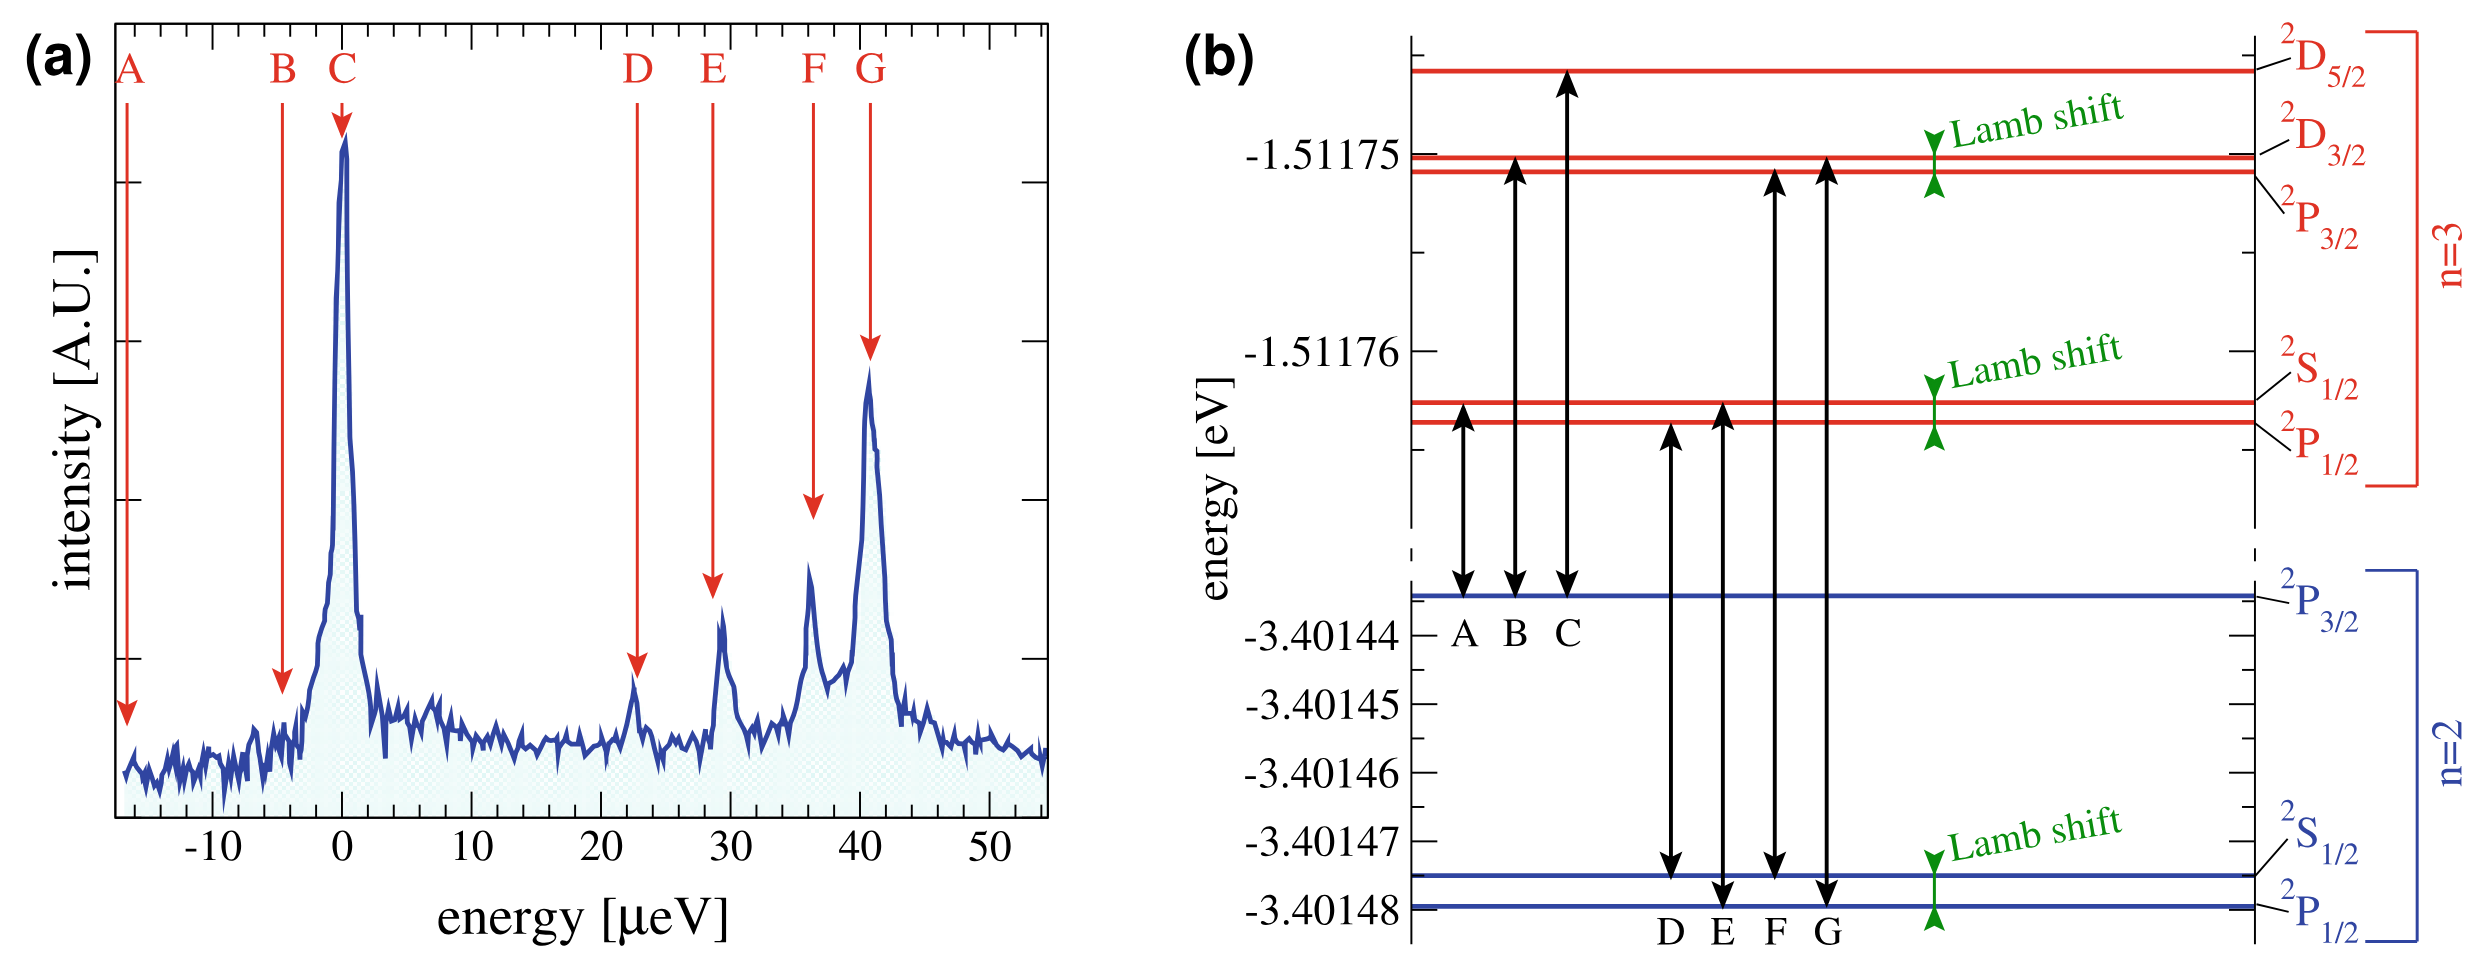
\includegraphics[width = 0.70 \textwidth]{lamb-shift.png}
	\caption{Lamb shift, both theoretical (b) and experimental (a), in the Balmer $ \ch{H}\alpha $ line.}
	\label{img:lamb}
\end{figure}

\section{Struttura iperfine}

Al pari degli elettroni, anche i nuclei hanno un momento angolare di spin $ \ve{I} $, e per molte specie nucleari esso è non-nullo (es.: per il protone $ i = \tfrac{1}{2} $). Per il momento magnetico nucleare sussiste la relazione:
\begin{equation}
	\bs{\mu}_n = g_n \mu_\text{N} \bs{i}
\end{equation}
dove $ \mu_\text{N} \equiv \frac{\hbar q_e}{2m_p} $ è il \textit{magnetone nucleare}. Il valore di $ g_n $ dipende dalla struttura interna del nucleo: ad esempio, per il protone $ g_n \simeq 5.58569 $.\\
Sebbene il campo magnetico nucleare, a parità di distanza, risulti soppresso di $ m_e / m_p \simeq 1 / 1836 $ rispetto a quello elettronico, attraverso questi i momenti magnetici nucleare ed elettronico interagiscono. Dato il fattore $ r^\ell $ in Eq. \ref{eq:1-e-radial}, elettroni con $ \ell > 0 $ hanno probabilità basse di trovarsi vicino al nucleo, dunque l'interazione con essi può essere ignorata; per quanto riguarda gli orbitali $ \ch{S} $, il campo magnetico elettronico è interamente generato dallo spin elettronico $ \ve{S} $ e, analogamente all'interazione spin-orbita, l'interazione tra spin elettronico e spin nucleare è descritta da:
\begin{equation*}
	\mathcal{H}_\text{s-n} = - C \bs{\mu}_n \cdot \bs{\mu}_e = C g_n g_s \mu_\text{N} \mu_\text{B} \bs{i} \cdot \bs{s}
	\qquad \qquad
	C = \frac{2}{3} \frac{1}{4\pi \epsilon_0 c^2} \abs{R_{n,0}(0)}^2 = \frac{2}{3\pi \epsilon_0 c^2} \left( \frac{Z}{an} \right)^3
\end{equation*}
Ricordando che per l'elettrone $ g_s = 2 $, la coupling energy caratteristica risulta essere:
\begin{equation}
	\xi_\text{N} = \frac{4}{3} g_n \frac{Z^3 \alpha^2}{n^3} \frac{m_e}{m_n} E_\text{Ha} \simeq g_n \frac{Z^3}{n^3} \times 1.05\,\mu\text{eV}
\end{equation}
Secondo le regole del momento angolare, $ \ve{I} $ ed $ \ve{S} $ si accoppiano in un \textit{momento angolare atomico} $ \ve{F} = \ve{I} + \ve{S} $, così che per il fattore $ \bs{i} \cdot \bs{s} $ valga, nella coupled basis ($ F^2 $ ed $ F_z $ diagonali), una relazione analoga ad Eq. \ref{eq:sl-coupled-basis}. Ricordando che $ s = \tfrac{1}{2} $, l'interazione tra momenti magnetici nucleare ed elettronico determina uno splitting tra i livelli iperfini $ f = i \pm \tfrac{1}{2} $ pari energeticamente a $ \xi_\text{N} (i \pm \tfrac{1}{2}) $.

\begin{example}{Riga $ 21\,\text{cm} $ dell'idrogeno}{}
	Per $ \ch{^1H} $ si ha $ i = \tfrac{1}{2} $, quindi $ \braket{\bs{i} \cdot \bs{s}} = - \tfrac{3}{4}, \tfrac{1}{4} $ per $ f = 0,1 $ rispettivamente. Nel ground state $ n = 1 $, dunque i due stati iperfini $ f = 0 $ ed $ f = 1 $ risulteranno separati di $ \xi_\text{N} \simeq 5.88\,\mu\text{eV} $: la transizione tra questi livelli sarebbe proibità, poiché $ \Delta \ell = 0 $, ma ha una probabilità non-nulla di avvenire tramite emissione di un fotone con $ \lambda = 2\pi \hbar c \xi_\text{N} \simeq 21\,\text{cm} $ e frequenza $ \nu = \xi_\text{N} (2\pi \hbar)^{-1} \simeq 1.42\,\text{GHz} $. Questa riga spettrale ha valenza storica, in quanto la lunga vita media della transizione (poiché proibita) ne ha permesso la misura della frequenza molto precisa, tant'è che per un periodo è stata usata come standard per l'unità di tempo.
\end{example}

\begin{example}{Struttura iperfine del cesio-137}{}
	Il $ \ch{^{137}Cs} $ è un nuclide con tutte le shell complete ed un elettrone ottico esterno, dunque può essere trattato come un atomo idrogenoide con $ i = \tfrac{7}{2} $ (nuclide dispari-pari). Di conseguenza, per il momento angolare atomico sono possibili solo due valori, dato che $ 3 \le f \le 4 $: la transizioni tra di essi produce un fotone di frequenza $ \nu = 9.192631770 \,\text{GHz} $, e questa riga spettrale e al momento utilizzata come standard per l'unità di tempo.
\end{example}

\section{Transizioni elettroniche}

\subsection{Decadimento spontaneo}

Quando un atomo viene eccitato, esso tenderà a decadere spontaneamente: sperimentalmente, si osserva che non tutte le transizioni procedono allo stesso rate, e ciò può essere spiegato da un'analisi quanto-meccanica dell'interazione del sistema col campo elettromagnetico ambientale. Nell'\textit{approssimazione di dipolo elettrico}\footnotemark, si trova che la probabilità di decadimento radiativo nell'unità di tempo da uno stato iniziale $ \ket{\text{i}} $ ad uno finale $ \ket{\text{f}} $ è:
\begin{equation}
	\gamma_\text{if} = \frac{1}{3\pi \epsilon_0 \hbar^4 c^3} \mathcal{E}_\text{if}^3 \abs{\braket{\text{f} | \ve{d} | \text{i}}}^2
	\label{eq:electron-trans-prob}
\end{equation}
con $ \mathcal{E}_\text{if} \equiv \hbar \omega_\text{if} \defeq E_\text{i} - E_\text{f} $ e $ \ve{d} \equiv - q_e \ve{r} $ l'operatore dipolo elettrico. La dipendenda dall'elemento di matrice $ \braket{\text{f} | \ve{d} | \text{i}} $ impone delle selection rules: le transizioni proibite avvengono con probabilità estremamente inferiori, dato che sono associate a termini di ordine superiore (in $ \alpha $) nell'espansione in multipolo (dipolo magnetico, quadrupolo elettrico, ...).

\footnotetext{Approssimazione valida nel caso in cui la sorgente della radiazione abbia dimensioni molto minori della lunghezza d'onda della radiazione emessa. Essendo $ k = \frac{2\pi}{\lambda} $ e $ \lambda = \frac{hc}{E} $, si ha $ k = \frac{E}{\hbar c} $, dunque tale approssimazione è valida, per $ E \sim 10 - 30 \ev $, se $ k \sim (100 \ang)^{-1} $. Inoltre, si noti che:
\begin{equation}
	\abs{\braket{\text{f} | \ve{p} | \text{i}}}^2 = \abs{\braket{\text{f} | \frac{m}{i\hbar} [\ve{r} , \mathcal{H}] | \text{i}}}^2 = \frac{m^2}{\hbar^2} (E_\text{i} - E_\text{f})^2 \abs{\braket{\text{f} | \ve{r} | \text{i}}}^2 = \frac{m^2}{\hbar^2 q_e^2} \mathcal{E}_\text{if}^2 \abs{\braket{\text{f} | \ve{d} | \text{i}}}^2
	\label{eq:electric-dipole-approx}
\end{equation}}

\begin{theorem}{Electric-dipole selection rule}{}
	Nell'approssimazione di dipolo elettrico per un atomo idrogenoide, le transizioni spontanee ammesse soddisfano:
	\begin{equation}
		\Delta \ell = \pm 1
	\end{equation}

	\tcblower
	
	\begin{proof}
		Esplicitando l'elemento di matrice di $ \ve{d} \equiv -q_e \ve{r} $ in funzione di quello di $ \ve{r} $:
		\begin{equation*}
			\abs{\braket{\text{f} | \ve{r} | \text{i}}}^2 = \abs{\braket{\text{f} | r_x | \text{i}}}^2 + \abs{\braket{\text{f} | r_z | \text{i}}}^2 + \abs{\braket{\text{f} | r_z | \text{i}}}^2
		\end{equation*}
		In funzione delle armoniche sferiche:
		\begin{align*}
			r_x &= r \sin \vartheta \cos \varphi = r \sqrt{\frac{2\pi}{3}} \left[ Y_{1,-1}(\vartheta, \varphi) - Y_{1,1}(\vartheta, \varphi) \right] \\
			r_y &= r \sin \vartheta \sin \varphi = r i \sqrt{\frac{2\pi}{3}} \left[ Y_{1,-1}(\vartheta, \varphi) + Y_{1,1}(\vartheta, \varphi) \right] \\
			r_z &= r \sqrt{\frac{4\pi}{3}} Y_{1,0}(\vartheta, \varphi)
		\end{align*}
		Ne segue che:
		\begin{equation*}
			\abs{\braket{\text{f} | \ve{r} | \text{i}}}^2 = \abs{\braket{\text{f} | r | \text{i}}}^2 \frac{4\pi}{3} \left[ \abs{\braket{\text{f} | Y_{1,-1} | \text{i}}}^2 + \abs{\braket{\text{f} | Y_{1,0} | \text{i}}}^2 + \abs{\braket{\text{f} | Y_{1,1} | \text{i}}}^2 \right]
		\end{equation*}
		Esplicitando in termini della funzione d'onda elettronica:
		\begin{equation*}
			\begin{split}
				\abs{\braket{n_\text{f} , \ell_\text{f} , m_\text{f} | \ve{d} | n_\text{i} , \ell_\text{i} , m_\text{i}}}^2
				& = q_e^2 \abs{\int_0^\infty \dd r\, r^2 R_{n_\text{f} , \ell_\text{f}}(r) R_{n_\text{i} , \ell_\text{i}}(r)}^2 \times \\
				& \times \frac{4\pi}{3} \sum_{m = -1,0,1} \abs{\int_0^\pi \dd \vartheta \, \sin \vartheta \int_0^{2\pi} \dd \varphi \, Y_{\ell_\text{f} , m_\text{f}}^*(\vartheta,\varphi) Y_{1,m}(\vartheta,\varphi) Y_{\ell_\text{i} , m_\text{i}}(\vartheta,\varphi)}^2
			\end{split}
		\end{equation*}
		L'integrale spaziale contribuisce soltanto allo smorzamento delle transizioni con $ \abs{n_\text{i} - n_\text{f}} $ grande, mentre la selection rule è imposta dall'integrale angolare: si noti che esso rappresenza l'overlap angolare tra $ Y_{\ell_\text{f} , m_\text{f}} $ e $ Y_{1,m} Y_{\ell_\text{i} , m_\text{i}} $, ma quest'ultimo può essere scomposto (secondo la decomposizione di Clebsch-Gordan) nella somma di stati con $ \ell = \abs{\ell_\text{i} - 1}, \ell_\text{i}, \ell_\text{i} + 1 $, dunque l'elemento di matrice è non-nullo sono per $ \ell_\text{f} = \ell $. Inoltre, si noti che l'integrale si annulla per $ \ell_\text{f} = \ell_\text{i} $: in tal caso, la parità dell'integranda sarebbe $ (-1)^{\ell_\text{i}} (-1)^1 (-1)^{\ell_\text{i}} = -1 $, dunque il suo integrale su tutto l'angolo solido è nullo. Gli unici valori possibili sono dunque $ \ell_\text{f} = \ell_\text{i} \pm 1 $, ovvero la selection rule cercata.
	\end{proof}
\end{theorem}

Essendo l'operatore dipolo elettrico associato a $ \ell = 1 $, si ha che $ m = -1,0,1 $; di conseguenza, si ottiene una selection rule anche sulla proiezione del momento angolare orbitale:
\begin{equation}
	\Delta m = 0, \pm 1
\end{equation}
Inoltre, dato che $ \ve{d} $ agisce come l'identità sullo spazio degli spin, si hanno:
\begin{equation}
	\Delta s = 0
	\qquad \qquad
	\Delta m_s = 0
	\label{eq:1-e-el-dip-tr-spin}
\end{equation}
È anche possibile esprimere la selection rule sulla base accoppiata, ottenendo:
\begin{equation}
	\Delta j = 0 , \pm 1
	\qquad \qquad
	\Delta m_j = 0 , \pm 1
\end{equation}
Una volta determinate le transizioni possibili, si può dare una stima del decay rate dall'Eq. \ref{eq:electron-trans-prob}, usando $ \mathcal{E}_\text{if} \simeq Z^2 E_\text{Ha} $ e $ \abs{\braket{\text{f} | \ve{d} | \text{i}}} = q_e a_0 / Z $:
\begin{equation*}
	\gamma_\text{if} = \frac{\mathcal{E}_\text{if}^3 \abs{\braket{\text{f} | \ve{d} | \text{i}}}^2}{3\pi \epsilon_0 \hbar^4 c^3} \simeq \frac{Z^4 E_\text{Ha}^2}{\epsilon_0 \hbar^4 c^3} \hbar \omega_\text{if} \frac{q_e^2 a_0^2}{Z^2} \simeq \frac{e^2 Z^2}{(\hbar c)^3} e^4 \omega_\text{if} = Z^2 \alpha^3 \omega_\text{if}
\end{equation*}
dato che $ E_\text{Ha} a_0 = e^2 $ e $ \alpha = e^2 / (\hbar c) $. Per un atomo idrogenoide $ \omega_\text{if} \simeq Z^2 \cdot 10^{16} \,\text{Hz} $, dunque si trova un tempo di decadimento dell'ordine $ \gamma_\text{if}^{-1} \simeq Z^{-4} \,\text{ns} $.

\begin{example}{Doppietto giallo del sodio}{}
	L'atomo di sodio presenta 11 elettroni: 10 interni in shell complete ed 1 esterno in 3s. Come in tutti gli altri atomi alcalini, l'elettrone esterno si trova più lontano dal nucleo rispetto alle shell interne ed è chiamato \textit{elettrone ottico}, poiché tipicamente le sue transizioni cadono nel visibile. Il potenziale a cui è soggetto l'elettrone ottico può essere visto come Coulombiano con un $ Z_\text{eff} $ efficacie: a grandi distanze dal nucleo $ Z_\text{eff} \simeq Z - (Z-1) = 1 $, mentre avvicinandosi ad esso $ Z_\text{eff} = Z_\text{eff}(r) $, il che rompe la degenerazione accidentale (l'energia è $ E = E(n,\ell) $). \\
	Nel caso del sodio, il tipico doppietto giallo del suo spettro d'emissione è dovuto alla transizione ottica ($ \Delta \ell = \pm 1 $) più piccola possibile per l'elettrone ottico, ovvero $ \text{3p} \rightarrow \text{3s} $ ($ \Delta E \sim 2\ev $). In particolare, sono presenti due righe a causa dell'interazione spin-orbita ($ \Delta E \sim 2.1 \,\text{meV} $), poiché le transizioni possibili sono due: $ \ch{^3P}_{3/2} \rightarrow \ch{^3S}_{1/2} $ ($ \lambda = 589.0 \,\text{nm} $) e $ \ch{^3P}_{1/2} \rightarrow \ch{^3S}_{1/2} $ ($ \lambda = 589.6 \,\text{nm} $).
\end{example}

\subsection{Decadimento stimolato}

In generale, un sistema immerso in un campo elettromagnetico descritto dai potenziali $ \phi $ ed $ \ve{A} $ è descritto dall'Hamiltoniana:
\begin{equation}
	\mathcal{H} = \frac{1}{2m} \left( \ve{p} - \frac{q}{c} \ve{A} \right)^2 + q \phi
\end{equation}
Nel caso dell'atomo idrogenoide:
\begin{equation}
	\mathcal{H} = \frac{1}{2m_e} \left( \ve{p} + \frac{e}{c} \ve{A} \right)^2 + \frac{1}{2M} \left( \ve{P} - \frac{Ze}{c} \ve{A} \right)^2 - \frac{Ze}{\abs{\ve{r} - \ve{R}}}
\end{equation}
Trascurando $ \frac{1}{M} \ll \frac{1}{m_e} $, ponendo $ \ve{R} = \ve{0} $ e scegliendo un gauge $ [\nabla , \ve{A}] = 0 $:
\begin{equation*}
	\begin{split}
		\mathcal{H}
		& \simeq \frac{1}{2m_e} \left( \ve{p} + \frac{e}{c} \ve{A} \right)^2 - \frac{Ze}{r} = \frac{1}{2m_e} \left[ -\hbar^2 \lap - i \frac{\hbar e}{c} (\nabla \cdot \ve{A} + \ve{A} \cdot \nabla) + \frac{e^2}{c^2} \ve{A}^2 \right] - \frac{Ze}{r} \\
		& = \frac{\hbar^2}{2m_e} \left[ -\lap - 2i \frac{\alpha}{e} \ve{A} \cdot \nabla + \frac{\alpha^2}{e^2} \ve{A}^2 \right] - \frac{Ze}{r} = \underbrace{- \frac{\hbar^2}{2m_e} \lap - \frac{Ze}{r}}_{\mathcal{H}_0} \underbrace{- i \frac{\hbar^2}{m_e} \frac{\alpha}{e} \ve{A} \cdot \nabla}_{V} + \underbrace{\frac{\hbar^2}{2m_e} \frac{\alpha^2}{e^2} \ve{A}^2}_{\sim \, \alpha^2}
	\end{split}
\end{equation*}
L'ultimo termine può essere trascurato, dunque il problema può essere trattato perturbativamente al prim'ordine (nell'approssimazione di campo debole). Per semplificare la trattazione, si adottano le unità atomiche $ \hbar = m_e = e = 1 , c = \alpha^{-1} \simeq 137 $:
\begin{equation}
	\mathcal{H} \simeq - \frac{1}{2} \lap - \frac{Z}{r} - i \alpha \ve{A} \cdot \nabla
\end{equation}
La dipendenza temporale degli autostati di $ \mathcal{H} $ non è più banale, in quanto la perturbazione determina una dipendenza temporale:
\begin{equation}
	\psi(t,r) = \sum_{n \in \N} c_n(t) e^{-i E_n t} \psi_n(r)
	\label{eq:1-e-pert-autof}
\end{equation}
dove $ \psi_n(r) $ sono gli stati stazionari di $ \mathcal{H}_0 $ e al prim'ordine:
\begin{equation}
	c_n(t) \simeq c_n^{(0)} + c_n^{(1)}(t)
	\label{eq:1-e-pert-coeff}
\end{equation}

\begin{proposition}{Coefficienti perturbativi}{}
	Per un potenziale del tipo:
	\begin{equation}
		\ve{A}(t,\ve{r}) = \ve{A}_0 e^{i (\ve{k}_0 \cdot \ve{r} - \omega_0 t + \varphi_0)} + \text{c.c.} = 2 \ve{A}_0 \cos (\ve{k}_0 \cdot \ve{r} - \omega_0 t + \varphi_0)
	\end{equation}
	i coefficienti nello sviluppo perturbativo per una transizione tra due stati stazionari $ \ket{n} , \ket{m} $ sono:
	\begin{equation}
		\begin{split}
			c_n^{(1)}(t) = - \alpha t \ve{A}_0 \cdot \bigg[
			& \ve{M}_{nm}(\ve{k}_0) \exp \left( i \frac{\omega_{nm} - \omega_0}{2} t + i \varphi_0 \right) \sinc \left( \frac{\omega_{nm} - \omega_0}{2} t \right) + \\
			& \qquad - \ve{M}_{mn}^*(\ve{k}_0) \exp \left( i \frac{\omega_{nm} + \omega_0}{2} t + i \varphi_0 \right) \sinc \left( \frac{\omega_{nm} + \omega_0}{2} t \right) \bigg]
			\label{eq:1-e-big-coeff}
		\end{split}
	\end{equation}
	con $ \ve{M}_{nm}(\ve{k}_0) \equiv \braket{n | e^{i \ve{k}_0 \cdot \ve{r}} \nabla | m} $.

	\tcblower

	\begin{proof}
		L'equazione di Schrödinger per l'autofunzione \ref{eq:1-e-pert-autof} diventa:
		\begin{equation*}
			\sum_{m \in \N} c_m(t) e^{-i E_m t} \mathcal{H} \psi_m(r) = i \sum_{m \in \N} \left[ \frac{dc_m(t)}{dt} - i E_m c_m(t) \right] e^{-i E_m t} \psi_m(r)
		\end{equation*}
		Moltiplicando a sinistra per $ \psi_n^*(r) $ ed integrando su tutto lo spazio:
		\begin{equation*}
			\sum_{m \in \N} c_m(t) e^{-i E_m t} \left( \delta_{nm} + \braket{n | V | m} \right) = \sum_{m \in \N} \left[ i \frac{dc_m(t)}{dt} + E_m c_m(t) \right] e^{-i E_m t} \delta_{nm}
		\end{equation*}
		Semplificando, si trova:
		\begin{equation*}
			\frac{dc_n(t)}{dt} = -i \sum_{m \in \N} c_m(t) e^{i \mathcal{E}_{nm} t} \braket{n | V | m}
		\end{equation*}
		Dall'Eq. \ref{eq:1-e-pert-coeff}, dato che $ c_n^{(1)} \ll c_n^{(0)} $:
		\begin{equation*}
			\frac{dc_n^{(1)}(t)}{dt} = -i \sum_{k \in \N} c_k^{(0)}(t) e^{i \mathcal{E}_{nk} t} \braket{n | V | k}
		\end{equation*}
		Per uno stato iniziale stazionario $ \ket{m} $ si ha $ c_k^{(0)} = \delta_{km} $, dunque:
		\begin{equation*}
			\frac{dc_n^{(1)}(t)}{dt} = -i e^{i \mathcal{E}_{nm} t} \braket{n | V | m} = - e^{i \mathcal{E}_{nm} t} \alpha \ve{A}_0 \cdot \left[ \braket{n | e^{i\ve{k}_0 \cdot \ve{r}} \nabla | m} e^{-i \omega_0 t + \varphi_0} + \text{c.c.} \right]
		\end{equation*}
		Essendo $ \nabla $ anti-hermitiano, $ \ve{M}_{nm}^*(\ve{k}_0) = - \ve{M}_{mn}(\ve{k}_0) $, ovvero:
		\begin{equation*}
			\frac{dc_n^{(1)}(t)}{dt} = - \alpha \ve{A}_0 \cdot \left[ \ve{M}_{nm}(\ve{k}_0) e^{i (\omega_{nm} - \omega_0) t + i \varphi_0} - \ve{M}_{mn}^*(\ve{k}_0) e^{i (\omega_{nm} + \omega_0) t - i \varphi_0} \right]
		\end{equation*}
		Integrando:
		\begin{equation*}
			\int_0^t dt' e^{i \beta t'} = \frac{e^{i\beta t} - 1}{i \beta} = \frac{i (1 - \cos \beta t) + \sin \beta t}{\beta} = \frac{2}{\beta} e^{i \beta \frac{t}{2}} \sin \left( \beta \tfrac{t}{2} \right) = \frac{t e^{i\beta \frac{t}{2}} \sin \left( \beta \frac{t}{2} \right)}{\beta \frac{t}{2}}
		\end{equation*}
		Utilizzando questo risultato per risolvere l'ODE per $ c_n^{(1)}(t) $ si ottiene la tesi.
	\end{proof}
\end{proposition}

Si ottiene quindi che, per un sistema inizialmente in uno stato stazionario $ \ket{m} $:
\begin{equation}
	\psi(t,r) = \psi_m(r) + \sum_{n \in \N} c_{nm}(t) e^{- i E_n t} \psi_n(r)
\end{equation}
con $ c_{nm}(t) \equiv c_n^{(1)}(t) $ come in Eq. \ref{eq:1-e-big-coeff}. La probabilità di transizione da $ \ket{m} $ a $ \ket{n} $, con $ n \neq m $, sarà dunque $ P_{nm}(t) = \abs{c_{nm}(t)}^2 $.

\paragraph{Risonanza}

Essendo $ \omega_0 $ la pulsazione della radiazione incidente, in base al valore di $ \omega_{nm} $ (differenza tra i due livelli energetici) si hanno due possibili risonanze (a seconda di quale termine domina in Eq. \ref{eq:1-e-big-coeff}):
\begin{itemize}
	\item $ \omega_{nm} \approx \omega_0 $: domina il primo termine, ovvero si ha risonanza per il processo di assorbimento (eccitamento) con transizione da $ \omega_m $ a $ \omega_n = \omega_m + \omega_0 $;
	\item $ \omega_{nm} \approx - \omega_0 $: domina il secondo termine, ovvero si ha risonanza per il processo di emissione (decadimento) con transizione da $ \omega_m $ a $ \omega_n = \omega_m - \omega_0 $.
\end{itemize}
Inoltre, si noti che $ \sinc{x} \rightarrow 0 $ per $ x \rightarrow \infty $, dunque col passare del tempo le probabilità di transizione per $ n \neq m $ tendono ad annullarsi; ciò è legato alla natura della radiazione emessa: inizialmente essa è non-monocromatica, ma col passare del tempo tende a diventare sempre più monocromatica.

\paragraph{Golden rule di Fermi}

È possibile definire la probabilità di transizione per unità di tempo sia nel caso dell'assorbimento che in quello dell'emissione:
\begin{align*}
	P_\text{a}(t) &= \abs{c_{nm}(t)}^2 \simeq \alpha^2 t^2 A_0^2 \abs{\bs{\epsilon} \cdot \ve{M}_{nm}(\ve{k}_0)}^2 \sinc^2 \left( \tfrac{\omega_{nm} - \omega_0}{2} t \right) \sim 2\pi \alpha^2 t A_0^2 \abs{\bs{\epsilon} \cdot \ve{M}_{nm}(\ve{k}_0)}^2 \delta(\tfrac{\omega_{nm} - \omega_0}{2}) \\
	P_\text{e}(t) &= \abs{c_{nm}(t)}^2 \simeq \alpha^2 t^2 A_0^2 \abs{\bs{\epsilon} \cdot \ve{M}_{mn}^*(\ve{k}_0)}^2 \sinc^2 \left( \tfrac{\omega_{nm} + \omega_0}{2} t \right) \sim 2\pi \alpha^2 t A_0^2 \abs{\bs{\epsilon} \cdot \ve{M}_{mn}^*(\ve{k}_0)}^2 \delta(\tfrac{\omega_{nm} + \omega_0}{2})
\end{align*}
dove $ \bs{\epsilon} = \ve{A}_0 / A_0 $ è la polarizzazione della radiazione incidente e $ \delta(x) = \frac{1}{2\pi} \lim_{t \rightarrow \infty} t \sinc^2(xt) $. Definendo l'intensità della radiazione incidente come $ I_0 \equiv A_0^2 \omega_0^2 / (2\pi c) $, si ottiene la golden rule di Fermi:
\begin{align*}
	P_\text{a}(t) &\simeq 4\pi \alpha^2 t \abs{\bs{\epsilon} \cdot \ve{M}_{nm}(\ve{k}_0)}^2 \frac{I_0}{\omega_0^2} \delta(\omega_{nm} - \omega_0) \\
	P_\text{e}(t) &\simeq 4\pi \alpha^2 t \abs{\bs{\epsilon} \cdot \ve{M}_{mn}^*(\ve{k}_0)}^2 \frac{I_0}{\omega_0^2} \delta(\omega_{nm} + \omega_0)
\end{align*}
Si noti che l'unico termine distinto è la $ \delta $ di conservazione dell'energia, la quale può essere scritta in maniera unificata come $ \delta(\omega_\text{f} - \omega_\text{i}) $. Inoltre, si vede che la probabilità di transizione diverge alla risonanza: questo però non è un problema, in quanto non esistono sorgenti puramente monocromatiche, in quanto dovrebbero emettere per un tempo infinito; più realisitcamente, si ha una distribuzione d'intensità attorno a $ \omega_0 $, così da scrivere:
\begin{equation*}
	\frac{I_0}{\omega_0^2} \delta(\omega_{nm} \pm \omega_0) \longrightarrow \int_{-\infty}^{+\infty} d\omega\, \frac{I(\omega)}{\omega^2} \delta(\omega_{nm} \pm \omega_0) = \frac{I(\omega_{nm})}{\omega_{nm}^2}
\end{equation*}
Utilizzando l'approssimazione di dipolo elettrico Eq. \ref{eq:electric-dipole-approx}, si trova che il rate di transizione $ \gamma_\text{if} \equiv P_\text{if} / t $ può essere scritto come:
\begin{equation*}
	\gamma_\text{if} = 4\pi \alpha^2 \abs{\braket{\text{f} | e^{i \ve{k}_0 \cdot \ve{r}} \nabla | \text{i}}}^2 \frac{I(\omega_\text{if})}{\omega_\text{if}^2} \simeq 4\pi \alpha^2 \abs{\braket{\text{f} | \ve{p} | \text{i}}}^2 \frac{I(\omega_\text{if})}{\omega_\text{if}^2} = 4\pi \alpha^2 \omega_\text{if}^2 \abs{\braket{\text{f} | \ve{d} | \text{i}}}^2 \frac{I(\omega_\text{if})}{\omega_\text{if}^2}
\end{equation*}
Si trova dunque:
\begin{equation}
	\gamma_\text{if} = 4\pi \alpha^2 I(\omega_\text{if}) \abs{\braket{\text{f} | \ve{d} | \text{i}}}^2
\end{equation}
A differenza dell'emissione spontanea, che è $ \sim \mathcal{E}_\text{if}^3 $, quella stimolata è $ \sim \mathcal{E}_\text{if}^2 $, dunque l'emissione spontanea diventa più probabile di quella stimolata all'aumentare della differenza energetica.

\section{Campo magnetico esterno}

Maggiori informazioni su una specie atomica possono essere ricavate immergendo il campione in un campo magnetico uniforme e studiandone lo spettro. Il momento magnetico atomico totale può essere scritto come:
\begin{equation}
	\bs{\mu} = \bs{\mu}_\ell + \bs{\mu}_s = - \mu_\text{B} ( g_\ell \bs{\ell} + g_s \bs{s}) \simeq - \mu_\text{B} (\bs{\ell} + 2 \bs{s})
\end{equation}
L'Hamiltoniana di coupling con un campo magnetico esterno, WLOG $ \ve{B} = B \hat{\ve{e}}_z $, è:
\begin{equation}
	\mathcal{H}_\text{magn} = - \bs{\mu} \cdot \ve{B} = \mu_\text{B} B (\ell_z + 2s_z)
\end{equation}
Si vede che $ \mathcal{H}_\text{magn} $ è diagonalizzabile nella uncoupled basis $ \ket{\ell, m, s, m_s} $, mentre $ \mathcal{H}_\text{s-o} $ lo è nella coupled basis $ \ket{\ell, s, j, m_j} $: dato che $ [\mathcal{H}_\text{magn} , \mathcal{H}_\text{s-o}] \neq 0 $, essi non sono simultaneamente diagonalizzabili, ma vanno diagonalizzati di volta in volta in ogni sottospazio $ (2\ell + 1)(2s + 1) $-dimensionale a $ n,\ell,s $ fissati.
È però possibile studiare i casi limite per le energie caratteristiche $ \mu_\text{B} B $ e $ \xi $.

\subsection{Limite Paschen-Back}

Nel limite $ \mu_\text{B} B \gg \xi $ in cui domina il campo magnetico esterno, la diagonalizzazione è diretta poiché si usa la uncoupled basis:
\begin{equation}
	\Delta E_\text{magn}(m,m_s) = \braket{m,m_s | \mathcal{H}_\text{magn} | m,m_s} = \mu_\text{B} B (m + 2m_s)
\end{equation}
mentre la correzione dovuta a $ \mathcal{H}_\text{s-o} $ può essere trattata perturbativamente. \\
Il valore di $ B $ per cui si può effettuare questa approssimazione dipende dall'atomo considerato e dal livello energetico: ad esempio, considerando la shell $ \text{2p} $, per $ \ch{H} $ si ha $ B \gg 0.5 \,\text{T} $, mentre per $ \ch{He}^+ $ si ha $ B \gg 8 \,\text{T} $, a causa della dipendenza da $ Z^4 $ in Eq. \ref{eq:1-e-int-spin-orb}.

\subsection{Limite Zeeman}

Il limite $ \mu_\text{B} B \ll \xi $ in cui domina l'interazione spin-orbita è quello più comune e in esso la simmetria sferica subisce solo una debole perturbazione. Gli stati $ \ket{\ell,s,j,m_j} $ nella coupled basis sono dunque autostati approssimati di $ \mathcal{H}_\text{s-o} + \mathcal{H}_\text{magn} $, mentre la correzione al prim'ordine dell'energia è:
\begin{equation}
	\Delta E_\text{magn}(j,m_j) \simeq \braket{j,m_j | \mathcal{H}_\text{magn} | j,m_j} = g_j \mu_\text{B} B m_j
\end{equation}
dove $ g_j $ è il fattore di Landé (Eq. \ref{eq:lande-g-factor}).

\subsection{Linee spettrali}

Sperimentalmente, si confermano le considerazioni teoriche sia esatte che approssimate. Prendendo ad esempio un campione di $ \ch{H} $, applicando un campo magnetico sufficientemente potente si osserva una triplicazione delle linee spettrali ($ \Delta m = 0, \pm 1 $), in accordo con l'effetto Paschen-Back, mentre applicando un campo magnetico debole si osserva l'effetto Zeeman (Fig. \ref{zeeman-effect}).

\begin{figure}
	\centering
	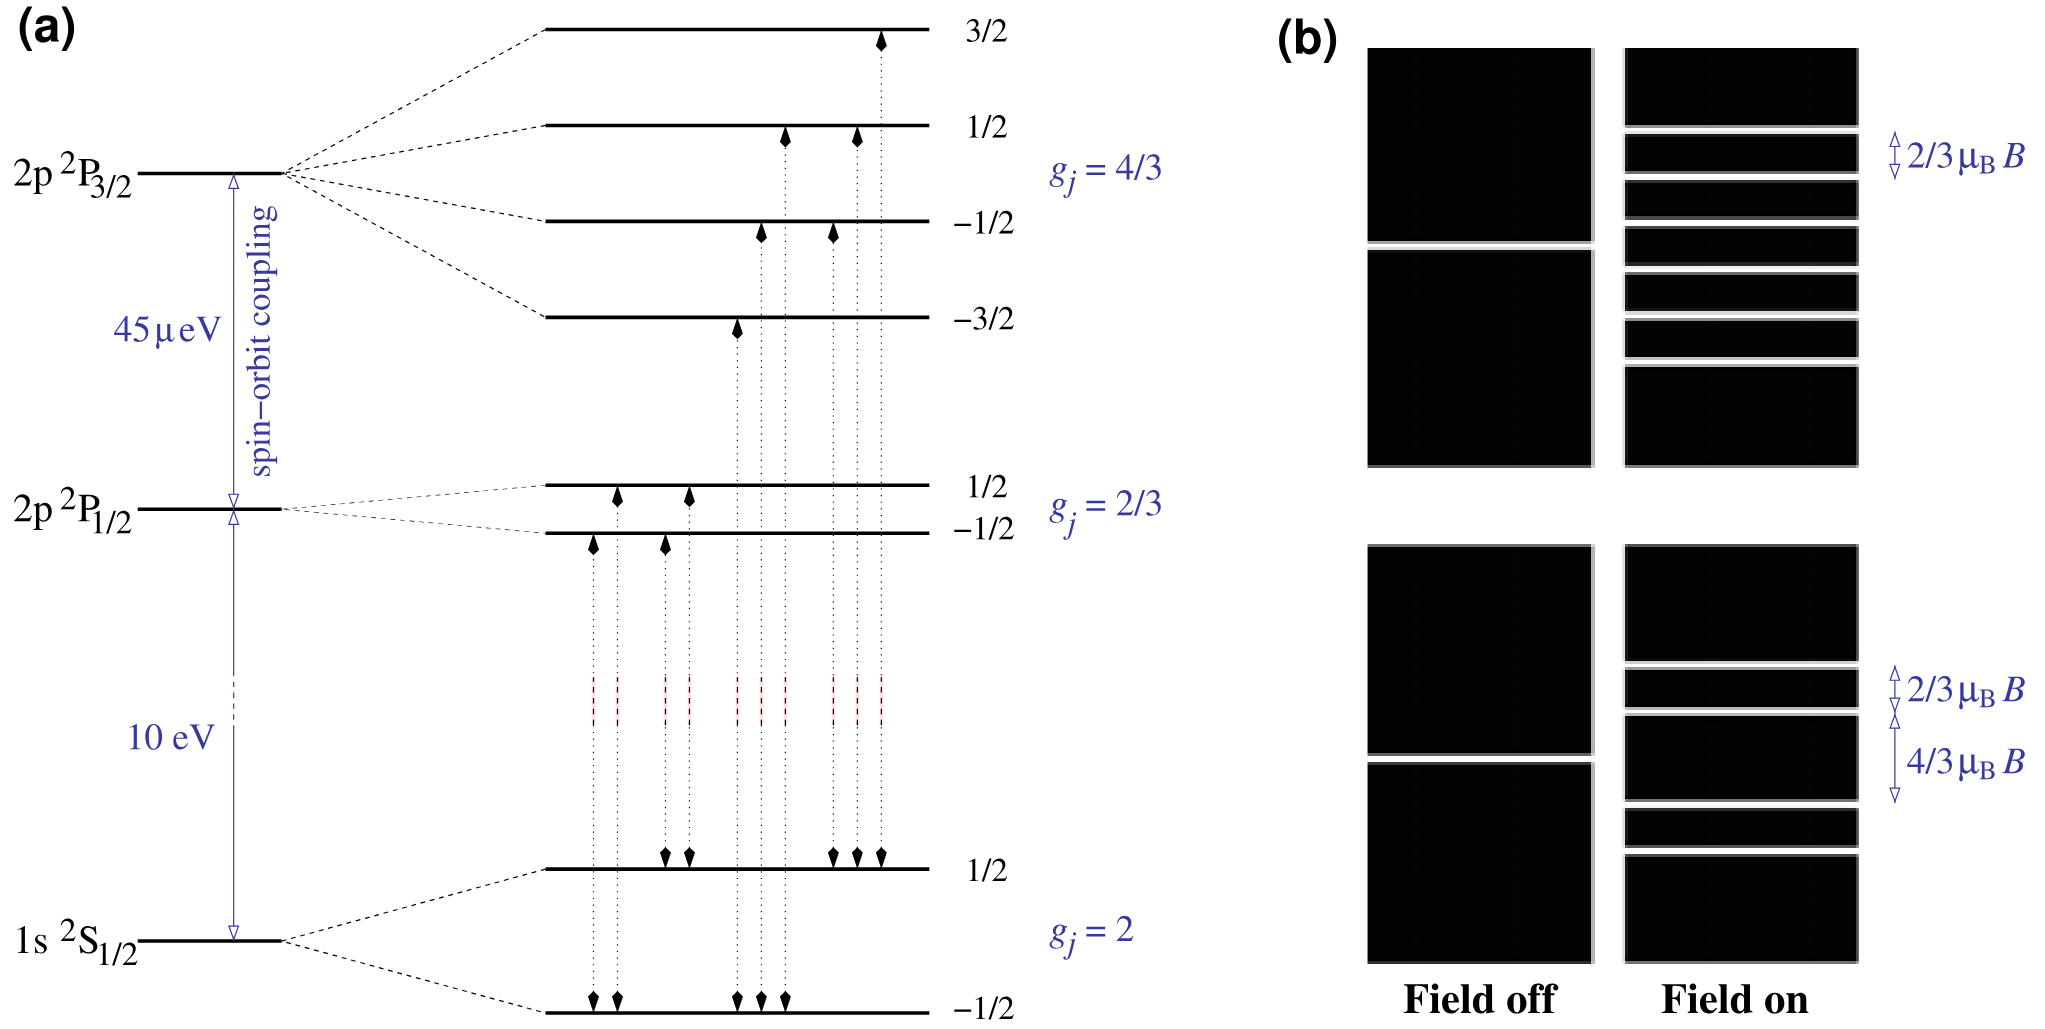
\includegraphics[width = 0.85 \textwidth]{zeeman-effect.png}
	\caption{Zeeman split of the lowest Lyman line of $ \ch{H} $.}
	\label{zeeman-effect}
\end{figure}

Nel regime intermedio $ \mu_\text{B} B \sim \xi $, nessuna delle due basi riesce a dare una descrizione accurata dei livelli energetici. Ad esempio, Fig. \ref{mag-field-int} mostra lo splitting pattern dei 6 stati $ \ch{^2P} $ in funzione dell'intensità del campo magnetico.

\begin{figure}[!b]
	\centering
	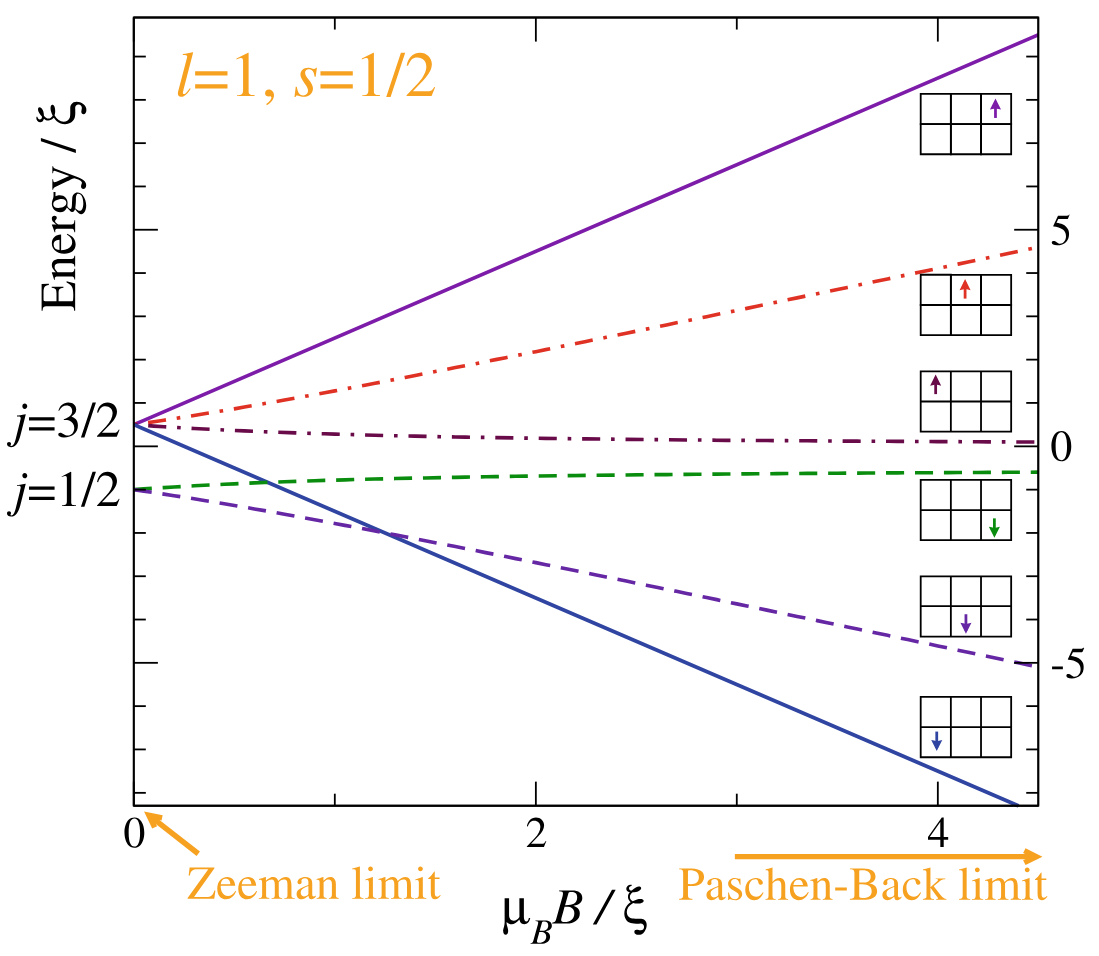
\includegraphics[width = 0.50 \textwidth]{mag-field-int.png}
	\caption{Combined spin-orbit and magnetic splittings of $ \ch{^2P} $.}
	\label{mag-field-int}
\end{figure}












\chapter{Atomi a Più Elettroni}
\selectlanguage{italian}

La trattazione degli atomi a molti elettroni (Many-Electron Atoms) è resa non banale dall'interazione elettrone-elettrone, la quale rende impossibile la risoluzione esatta del problema\footnotemark. È dunque necessario adottare alcune semplificazioni.

\footnotetext{La funzione d'onda di ciascun elettrone dipende da tre variabili spaziali, dunque, discretizzando ciascuna di esse in una griglia di 10 numeri reali, la descrizione di un sistema a $ N $ elettroni richiede di trattare $ (10^3)^N $ numeri reali: già per $ N = 4 $ ciò necessiterebbe di qualche Tb, mentre per $ N = 27 $ si raggiunge l'ordine di grandezza del numero totale di atomi nell'Universo. La trattazione numerica del problema è dunque impossibile.}

\section{Approssimazione a particelle indipendenti}

È possibile trovare soluzioni approssimate per MEAs costruendo il relativo spazio di Hilbert a partire dagli stati single-particle.

\subsection{Particelle identiche}

Gli elettroni sono particelle indistinguibili tra loro, dunque è necessario ricordare le proprietà dei sistemi quantistici di particelle identiche. \\
Dato un sistema di $ N $ particelle identiche, ciascuna descritta da uno spazio di Hilbert $ \hilb $, il sistema totale sarà descritto da un sottospazio del prodotto diretto di tali spazi. In particolare, definendo l'operatore di scampio $ \pi_{ij} $ che scambia le particelle $ i \leftrightarrow j $, dato che $ \pi_{ij}^2 $ si ha che i suoi autovalori possibili sono $ \pm 1 $: stati $ \pi_{ij} \ket{\psi} = + \ket{\psi} $ sono detti \textit{stati bosonici}, sono simmetrici per scambio di particelle e descrivono sistemi di spin intero; stati $ \pi_{ij} \ket{\psi} = - \ket{\psi} $ sono detti \textit{stati fermionici}, sono antisimmetrici per scambio di particelle e descrivono sistemi di spin semi-intero. La definizione degli stati bosonici/fermionici a partire dagli stati single-particle è dunque data rispettivamente da:
\begin{equation}
	\ket{\alpha_1 , \dots , \alpha_N}^\text{(s)} \defeq \frac{1}{\sqrt{N!}} \sum_{\pi \in S^N} \ket{\alpha_{\pi(1)} , \dots , \alpha_{\pi(N)}}
\end{equation}
\begin{equation}
	\ket{\alpha_1 , \dots , \alpha_N}^\text{(a)} \defeq \frac{1}{\sqrt{N!}} \sum_{\pi \in S^N} (-1)^{\{\pi\}} \ket{\alpha_{\pi(1)} , \dots , \alpha_{\pi(N)}}
\end{equation}
dove $ \{\pi\} $ è il carattere della permutazione e $ \alpha_n $ indica il set completo di quantum numbers dell'$ n $-esima particella. Come si può vedere, il principio d'esclusione di Pauli discende banalmente da queste definizioni: un sistema bosonico non ha restrizioni sui quantum numbers dei singoli bosoni che lo compongono, mentre un sistema fermionico, dato il fattore $ (-1)^{\{\pi\}} $, risulta avere $ \ket{\psi} = 0 $ se si considerano due fermioni con gli stessi quantum numbers.

\begin{example}{Identicità degli atomi}{}
	Si consideri un atomo di $ \ch{^3He} $: esso è composto da 2 protoni, 1 neutrone e 2 elettroni, dunque overall è un sistema fermionico: se si scambiano tra loro due tali atomi, si ottiene un fattore $ (-1)\cdot(-1) = +1 $ per i protoni, idem per gli elettroni, e $ (-1) $ per i neutroni, risultando in un fattore totale $ (-1) $. \\
	D'altro canto, un atomo di $ \ch{^{238}U} $, composto da 92 protoni, 146 neutroni e 92 elettroni, è un sistema bosonico per un ragionamento analogo. \\
	In generale, atomi con $ A + Z $ pari sono bosoni, mentre atomi con $ A + Z $ dispari sono fermioni.
\end{example}

L'antisimmetria per scambio dei sistemi a molti elettroni ne condiziona fortemente al dinamica, in quanto la repulsione tra elettroni data dall'antisimettrizzazione della funzione d'onda è spesso più efficace della repulsione elettromagnetica tra di essi: senza antisimmetria, gli elettroni nel ground state occuperebbero tutti la shell $ \text{1s} $.

\subsubsection{Funzione d'onda fermionica}

Si consideri un sistema di $ N $ fermioni, ciascuno descritto da uno spazio di Hilbert con ket base $ \ket{w_n} = \ket{\ve{r}_n , \sigma_n} $ di posizione e spin.

\begin{theorem}{Determinante di Slater}{}
	La base dello spazio di Hilbert di un sistema di $ N $ fermioni è data dal \textit{determinante di Slater}:
	\begin{equation}
		\Psi_{\alpha_1 , \dots , \alpha_N}(w_1 , \dots , w_N) = \frac{1}{\sqrt{N!}}
		\begin{vmatrix}
			\psi_{\alpha_1}(w_1) & \dots & \psi_{\alpha_1}(w_N) \\
			\vdots & \ddots & \vdots \\
			\psi_{\alpha_N}(w_1) & \dots & \psi_{\alpha_N}(w_N)
		\end{vmatrix}
	\end{equation}

	\tcblower

	\begin{proof}
		Essendo lo spazio di Hilbert totale $ \hilb^\text{(a)} $, la funzione d'onda dello stato fermionico generico $ \ket{\alpha_1 , \dots , \alpha_N}^\text{(a)} $ sarà:
		\begin{equation*}
			\begin{split}
				\Psi_{\alpha_1 , \dots , \alpha_N}(w_1 , \dots , w_N)
				& = {^\text{(a)}\langle}w_1 , \dots , w_N | \alpha_1 , \dots , \alpha_N{\rangle^\text{(a)}} \\
				& = \frac{1}{N!} \sum_{\pi,\rho \in S^N} (-1)^{\{\pi\}} (-1)^{\{\rho\}} \braket{w_{\rho(1)} , \dots , w_{\rho(N)} | \alpha_{\pi(1)} , \dots , \alpha_{\pi(N)}} \\
				& = \sum_{\pi \in S^N} (-1)^{\{\pi\}} \frac{1}{N!} \sum_{\rho \in S^N} (-1)^{\{\rho\}} \psi_{\alpha_{\pi(1)}}(w_{\rho(1)}) \dots \psi_{\alpha_{\pi(N)}}(w_{\rho(N)}) \\
				& = \sum_{\pi \in S^n} (-1)^{\{\pi\}} \psi_{\alpha_{\pi(1)}}(w_1) \dots \psi_{\alpha_{\pi(N)}}(w_N)
			\end{split}
		\end{equation*}
		Questa è proprio la definizione di determinante della matrice $ A_{ij} = \psi_{\alpha_i}(w_j) $. Aggiungendo un fattore di normalizzazione $ (N!)^{-1/2} $ si ottiene la tesi\footnote{Ciò permette di usare come dominio d'integrazione tutto lo spazio di definizione delle $ w_n $, e non solo l'iper-triangolo $ w_1 > \dots > w_n $.}.
	\end{proof}
\end{theorem}

In questo modo diventa possibile trattare numericamente il problema\footnotemark. La complessità del problema viene relegata ai coefficienti dell'espansione dello stato generico su tale base:
\begin{equation}
	\ket{\Psi} = \sum_{\alpha_1 , \dots , \alpha_N} c_{\alpha_1 , \dots , \alpha_N} \ket{\alpha_1 , \dots , \alpha_N}^\text{(a)}
\end{equation}
con $ c_{\alpha_1 , \dots , \alpha_N} \in \C $. In questo modo, dunque, si ottiene lo stato del sistema totale a partire dagli stati single-particle: da qui l'\textit{approssimazione a particelle indipendenti}.

\footnotetext{I ket di base ottenuti tramite il determinante di Slater contengono una quantità d'informazione che, seguengo l'esempio della nota precedente, scala come $ N \cdot 10^3 $, dunque linearmente.}

\subsection{Elettroni non-interagenti}

Si consideri il potenziale d'interazione elettrone-elettrone $ V_{ee} $ completamente trascurabile: in tal caso, il problema ad $ N $ elettroni si fattorizza completamente, poiché ciascun elettrone si muove indipendentemente dagli altri nel potenziale $ V_{ne} $. Trascurando gli effetti relativistici, gli autostati dei singoli elettroni sono rappresentati dalla funzione d'onda idrogenoide\footnotemark: si ha dunque $ \alpha_i \equiv \{n_i, \ell_i, m_i, m_{s_i}\} $.

\footnotetext{Nel caso dei MEAs, si può ignorare la dimensione finita del nucleo, assumendo $ \mu \equiv m_e $ e $ a \equiv a_0 $.}

\begin{example}{Notazione spettroscopica}{}
	In notazione spettroscopica si perde l'informazione su $ m_i $ ed $ m_{s_i} $. Ad esempio:
	\begin{equation*}
		\ket{1,0,0,\uparrow ; 3,1,-1,\uparrow ; 3,1,0,\uparrow ; 3,1,1,\downarrow}^\text{(a)} \equiv \text{1s}^1 \text{3p}^3
	\end{equation*}
\end{example}

\subsubsection{Energia totale}

La binding energy di un atomo è definita come il lavoro necessario a separare l'atomo in un nucleo isolato e nei suoi $ N $ elettroni, tutti a riposo e all'infinito. La sua energia totale è invece $ E = - E_\text{bind} $. \\
Nel caso di elettroni non-interagenti, l'energia totale è semplicemente la somma delle loro singole energie (che sono negative).

\begin{example}{}{}
	L'energia dello stato $ \text{1s}^1 \text{3p}^3 $ è (dall'Eq. \ref{eq:1-e-en}:
	\begin{equation*}
		E[\text{1s}^1 \text{3p}^3] = E_1 + 3 E_3 = - \frac{1}{2} \left( \frac{1}{1^2} + 3 \cdot \frac{1}{3^2} \right) Z^2 E_\text{Ha} = - \frac{2}{3} Z^2 E_\text{Ha}
	\end{equation*}
	Gli stati ad energia minima per un sistema di $ N = 4 $ elettroni sono però quelli con $ 2 $ elettroni in $ n = 1 $ (massimo numero nell'unica shell con $ n = 1 $, ovvero $ \text{1s} $) e $ 2 $ elettroni in $ n = 2 $; ad esempio:
	\begin{equation*}
		E[\text{1s}^2 \text{2s}^2] = 2 E_1 + 2 E_2 = - \frac{5}{4} Z^2 E_\text{Ha}
	\end{equation*}
\end{example}

\subsubsection{Elettroni reali}

In sistemi reali, l'approssimazione $ V_{ee} \equiv 0 $ può risultare estremamente fallace: ad esempio, per un atomo neutro in cui $ N = Z $ si ha che $ V_{ee} $ è dello stesso ordine di grandezza, ma di segno opposto, di $ V_{ne} $, così da cancellarne gli effetti: in tal caso, trascurare $ V_{ee} $ porterebbe a risultati fisicamente insensati.

\section{Atomi a 2 elettroni}

Gli atomi polielettronici più semplici sono quelli con $ N = 2 $ (es.: $ \ch{He} $, $ \ch{Li}^+ $, $ \ch{Be}^{2+} $, ...). L'Hamiltoniana di questo sistema è:
\begin{equation*}
	\mathcal{H} = T + V_{ne} + V_{ee} = - \frac{\hbar^2}{2m_e} \lap_1 - \frac{\hbar^2}{2m_e} \lap_2 - \frac{Ze^2}{r_1} - \frac{Ze^2}{r_2} + \frac{e^2}{\abs{\ve{r}_1 - \ve{r}_2}} = \mathcal{H}_1 + \mathcal{H}_2 + V_{ee}
\end{equation*}
Questa Hamiltoniana è resa non-fattorizzabile dal termine $ V_{ee} $, il quale può però essere trattato perturbativamente nel caso $ N = 2 $; per $ N \ge 3 $, invece, bisogna tener conto della schermatura del potenziale $ V_{ne} $ da parte di quello $ V_{ee} $. \\
La funzione d'onda per elettroni indipendenti ($ V_{ee} \equiv 0 $) in questo è:
\begin{equation*}
	\Psi_{\alpha_1 , \alpha_2}(w_1 , w_2) = \frac{1}{\sqrt{2}} \left[ \psi_{\alpha_1}(w_1) \psi_{\alpha_2}(w_2) - \psi_{\alpha_1}(w_2) \psi_{\alpha_2}(w_1) \right]
\end{equation*}
con:
\begin{equation*}
	\psi_{\alpha_i}(w_i) = R_{n_i, \ell_i}(r_i) Y_{\ell_i, m_i}(\vartheta_i, \varphi_i) \chi_{m_{s_i}}(\sigma_i) \equiv \psi_{n_i, \ell_i, m_i}(\ve{r}_i) \chi_{m_{s_i}}(\sigma_i)
\end{equation*}
Si nota però che gli stati $ \Psi_{\alpha_1, \alpha_2} $ così definiti non sono necessariamente autostati dello spin totale $ S^2 $ (con $ \bs{S} \defeq \bs{s}_1 + \bs{s}_2 $): è utile lavorare con autostati di $ S^2 $, poiché la perturbazione $ V_{ee} \equiv V_{ee} \otimes \id_\text{spin} $ agisce solo sullo spazio orbitale, dunque il suo elemento di matrice si annulla tra stati con $ S $ diverso. \\
Per ottenere tali autostati, è utile separare la parte spaziale della funzione d'onda da quella di spin: si ottengono così un singoletto $ S = 0 $ (con funzione d'onda di spin antisimmetrica) ed un tripletto simmetrico $ S = 1 $ (con funzione d'onda di spin simmetrica). Si definiscono i relativi spinori $ \mathcal{X}^{S,M_S} $:
\begin{align*}
	\mathcal{X}^{0,0}(\sigma_1, \sigma_2) &= \frac{1}{\sqrt{2}} \left[ \chi_\uparrow(\sigma_1) \chi_\downarrow(\sigma_2) - \chi_\uparrow(\sigma_2) \chi_\downarrow(\sigma_1) \right] \\
	\mathcal{X}^{1,-1}(\sigma_1, \sigma_2) &= \chi_\downarrow(\sigma_1) \chi_\downarrow(\sigma_2) \\
	\mathcal{X}^{1,0}(\sigma_1, \sigma_2) &= \frac{1}{\sqrt{2}} \left[ \chi_\uparrow(\sigma_1) \chi_\downarrow(\sigma_2) + \chi_\uparrow(\sigma_2) \chi_\downarrow(\sigma_1) \right] \\
	\mathcal{X}^{1,1}(\sigma_1, \sigma_2) &= \chi_\uparrow(\sigma_1) \chi_\downarrow(\sigma_2)
\end{align*}
Le parti spaziali devono essere coerentemente (anti)simmetrizzate, così da ottenere:
\begin{equation*}
	\Psi^{0,0}_{n_1, \ell_1, m_1 ; n_2, \ell_2, m_2}(w_1, w_2) = \frac{1}{\sqrt{2}} \left[ \psi_{n_1, \ell_1, m_1}(\ve{r}_1) \psi_{n_2, \ell_2, m_2}(\ve{r}_2) + \psi_{n_1, \ell_1, m_1}(\ve{r}_2) \psi_{n_2, \ell_2, m_2}(\ve{r}_1) \right] \mathcal{X}^{0,0}(\sigma_1, \sigma_2)
\end{equation*}
\begin{equation*}
	\Psi^{1,M_S}_{n_1, \ell_1, m_1 ; n_2, \ell_2, m_2}(w_1, w_2) = \frac{1}{\sqrt{2}} \left[ \psi_{n_1, \ell_1, m_1}(\ve{r}_1) \psi_{n_2, \ell_2, m_2}(\ve{r}_2) - \psi_{n_1, \ell_1, m_1}(\ve{r}_2) \psi_{n_2, \ell_2, m_2}(\ve{r}_1) \right] \mathcal{X}^{1,M_S}(\sigma_1, \sigma_2)
\end{equation*}
Gli stati dello spin-singlet non hanno condizioni sui quantum numbers orbitali, ma devono necessariamente avere $ m_{s_1} = - m_{s_2} $, mentre, al contrario, gli stati dello spin-triplet non hanno condizioni sui quantum numbers di spin, ma devono avere $ (n_1,\ell_1,m_1) \neq (n_2,\ell_2,m_2) $.

\subsection{Stati eccitati}

Trascurando l'interazione elettronica, le energie non-pertubate dipendono solo da $ n_1,n_2 $:
\begin{equation*}
	E_{n_1,n_2}^{(0)} = - \frac{1}{2} \left( \frac{1}{n_1^2} + \frac{1}{n_2^2} \right) Z^2 E_\text{Ha}
\end{equation*}
Si vede che il ground state è uno stato dello spin-singlet: infatti esso ha entrambi gli elettroni in $ \text{1s} $, dunque $ \uparrow\downarrow $ o $ \downarrow\uparrow $, ovvero descritti da $ \mathcal{X}^{0,0} $. \\
Ricordando le selection rules sullo spin per le transizioni di dipolo elettrico (Eq. \ref{eq:1-e-el-dip-tr-spin}), si vede che queste avvengono soltanto tra stati appartenenti entrambi al singoletto o entrambi al tripletto, come si può vedere in Fig. \ref{helium} nel caso dell'elio: storicamente, si pensava ci fossero due specie distinte di elio, l'orto-elio ($ S = 1 $) ed il para-elio ($ S = 0 $).

\begin{figure}
	\centering
	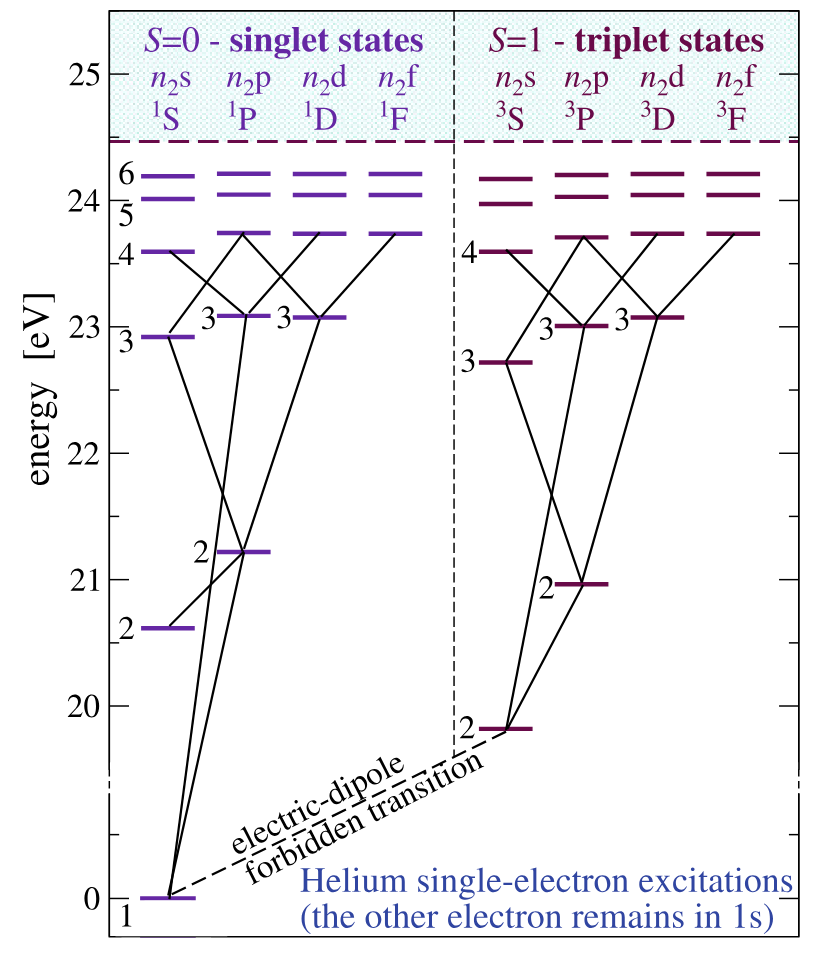
\includegraphics[width = 0.40 \textwidth]{ortho-para-he.png}
	\caption{Energy levels and electric-dipole transitions of atomic $ \ch{He} $.}
	\label{helium}
\end{figure}

\subsection{Elettroni interagenti}
\label{he-inter-electr}

Trattando in maniera perturbativa il potenziale d'interazione $ V_{ee} $, al prim'ordine si ha una correzione all'energia (nelle configurazioni para- o orto-) data da:
\begin{equation*}
	\begin{split}
		\Delta E_{k_1,k_2}^\text{(p,o)}
		& = \braket{\Psi_{k_1,k_2}^\text{(p,o)} | V_{ee} | \Psi_{k_1,k_2}^\text{(p,o)}} = \frac{e^2}{2} \int_{\R^6} \frac{d^3r_1 d^3r_2}{\abs{\ve{r}_1 - \ve{r}_2}}  \abs{\psi_{k_1}(\ve{r}_1) \psi_{k_2}(\ve{r}_2) \pm \psi_{k_1}(\ve{r}_2) \psi_{k_2}(\ve{r}_1)}^2 \\
		& = \frac{e^2}{2} \int_{\R^6} \frac{d^3r_1 d^3r_2}{\abs{\ve{r}_1 - \ve{r}_2}} \left[ \abs{\psi_{k_1}(\ve{r}_1)}^2 \abs{\psi_{k_2}(\ve{r}_2)}^2 + \abs{\psi_{k_1}(\ve{r}_2)}^2 \abs{\psi_{k_2}(\ve{r}_1)}^2 \right] \\
		& \quad \pm \frac{e^2}{2} \int_{\R^6} \frac{d^3r_1 d^3r_2}{\abs{\ve{r}_1 - \ve{r}_2}} \left[ \psi_{k_1}^*(\ve{r}_1) \psi_{k_2}^*(\ve{r}_2) \psi_{k_1}(\ve{r}_2) \psi_{k_2}(\ve{r}_1) + \psi_{k_1}(\ve{r}_1) \psi_{k_2}(\ve{r}_2) \psi_{k_1}^*(\ve{r}_2) \psi_{k_2}^*(\ve{r}_1) \right] \\
		& \equiv E_{k_1,k_2}^\text{(c)} \pm E_{k_1,k_2}^\text{(s)}
	\end{split}
\end{equation*}
dove $ k_i \equiv \{n_i,\ell_i,m_i\} $. $ E^\text{(c)} $ è l'energia dovuta all'interazione Coulombiana, mentre $ E^\text{(s)} $ è dovuta all'interazione di scambio: si dimostra che $ E^\text{(s)} \ge 0 $, dunque la configurazione para- ha un'energia superiore a quella orto- (come si vede in Fig. \ref{helium}). \\
Il fatto che la configurazione orto- sia energeticamente inferiore a quella para- può anche essere dedotto intuitivamente dalla simmetria della funzione d'onda: nel caso orto-, poiché la funzione d'onda spaziale è antisimmetrica, si ha $ \psi(\ve{r},\ve{r}) = 0 $, dunque è molto meno probabile che i due elettroni si trovino vicini rispetto al caso para-. Poiché $ V_{ee} \sim \abs{\ve{r}_1 - \ve{r}_2}^{-1} $, ciò significa che la correzione al prim'ordine dell'energia sarà maggiore nel caso para- rispetto a quello orto-. \\
Gli stati $ (n_1[\ell_1])(n_2[\ell_2]) $ subiscono dunque uno splitting energetico pari a $ 2E^\text{(s)}_{n_1,\ell_1 ; n_2,\ell_2} $ (la dipendenza da $ m $ c'è solo in presenza di campi elettromagnetici esterni che perturbano la simmetria sferica), noto come \textit{splitting da scambio}. Questo splitting è molto importante, poiché sta alla base della \textit{prima regola di Hund}: lo stato energeticamente più basso è sempre quello che massimizza lo spin\footnotemark.

\footnotetext{Ciò nel caso dell'atomo a 2 elettroni non ha alcun effetto sul ground state, poiché esso ha configurazione elettronica $ \text{1s}^2 $, dunque necessariamente $ S = 0 $.}

\section{Atomi a \texorpdfstring{$ N $}{N} elettroni}

L'approccio perturbativo non dà un buon accordo coi dati sperimentali per $ N \ge 3 $: di conseguenza, è necessario adottare un altro metodo. Un'opzione è sfruttare il principio di Ritz (Th. \ref{th:ritz}): supponendo di avere un set di autofunzioni single-particle $ \{\phi_{\alpha_i}(w_i)\}_{i = 1, \dots, N} $ note, è possibile cercare un set di autofunzioni che fungono da base per lo spazio di Hilbert del sistema considerato andando a minimizzare il funzionale energia:
\begin{equation}
	E[\phi_{\alpha_1}, \dots, \phi_{\alpha_N}] = \frac{\braket{\Phi_{\alpha_1, \dots, \alpha_N} | \mathcal{H}_\text{MEA} | \Phi_{\alpha_1, \dots, \alpha_N}}}{\braket{\Phi_{\alpha_1, \dots, \alpha_N} | \Phi_{\alpha_1, \dots, \alpha_N}}}
	\label{eq:en-functional-def}
\end{equation}
dove $ \Phi_{\alpha_1, \dots, \alpha_N} $ è il determinante di Slater delle $ {\phi_{\alpha_i}}_{i = 1, \dots, N} $, le quali sono dette \textit{orbitali atomici}. Essendo $ \mathcal{H}_\text{MEA} = T + V_{ne} + V_{ee} $, si può esplicitare il funzionale come:
\begin{equation}
	\begin{split}
		E[\phi_{\alpha_1}, \dots, \phi_{\alpha_N}]
		& = \sum_{i = 1}^{N} \braket{\alpha_i | \mathcal{H}_0 | \alpha_i} \\
		& \quad + \frac{1}{2} \sum_{i,j = 1}^{N} \int dw\,dw'\, \abs{\phi_{\alpha_i}(w)}^2 v_{ee}(w,w') \abs{\phi_{\alpha_j}(w')}^2 \\
		& \quad - \frac{1}{2} \sum_{i,j = 1}^{N} \int dw\,dw'\, \phi_{\alpha_i}^*(w) \phi_{\alpha_i}(w') v_{ee}(w,w') \phi_{\alpha_j}^*(w') \phi_{\alpha_j}(w)
	\end{split}
	\label{eq:en-functional}
\end{equation}
dove si è assunta l'ortonormalità $ \braket{\alpha_i | \alpha_j} = \delta_{ij} $ e si sono definiti:
\begin{equation}
	\mathcal{H}_0(w) \equiv \left[ -\frac{\hbar^2}{2m_e} \lap_\ve{r} - \frac{Ze^2}{r} \right] \otimes \id_\text{spin}
	\qquad \qquad
	v_{ee}(w,w') \equiv \frac{e^2}{\abs{\ve{r} - \ve{r}'}} \otimes \id_\text{spin}
\end{equation}
Il primo termine del funzionale energia contiene il moto indipendente di ogni elettrone nel potenziale generato dal nucleo, il secondo termine contiene l'interazione Coulombiana tra ciascun elettrone ed la distribuzione di carica media dovuta a tutti gli elettroni, e il terzo termine è un termine di natura non-classica e non-locale dovuto all'antisimmetria per scambio: si noti che il secondo termine contiene anche un'interazione di ciascun elettrone con sé stesso, la quale non ha senso fisico, che viene giustamente cancellata da un addendo nel terzo termine.

\begin{theorem}{Equazione di Hartree-Fock}{eq-hf}
	Il set di autofunzioni $ \{\psi_{\alpha_i}\}_{i = 1, \dots, N} $ che minimizza il funzionale energia soddisfa:
	\begin{equation}
		\mathcal{H}_0(w) \psi_\alpha(w) + V_\text{Ha}(w) \psi_\alpha(w) - \int dw'\, V_\text{Fock}(w,w') \psi_\alpha(w') = E_\alpha \psi_\alpha(w)
	\end{equation}
	dove i potenziali di Hartree e Fock sono definiti come:
	\begin{equation}
		V_\text{Ha}(w) \defeq \int dw'\, \sum_\beta \abs{\phi_\beta(w')}^2 v_{ee}(w,w')
	\end{equation}
	\begin{equation}
		V_\text{Fock}(w,w') \defeq \sum_\beta \phi_\beta^*(w') \phi_\beta(w) v_{ee}(w,w')
	\end{equation}

	\tcblower

	\begin{proof}
		Partendo dall'Eq. \ref{eq:en-functional-def}, si noti che in generale:
		\begin{equation*}
			\frac{\pa E(p)}{\pa p_i} = \frac{\pa}{\pa p_i} \frac{N(p)}{D(p)} = 0
			\quad \Leftrightarrow \quad
			\frac{1}{D(p)} \frac{\pa N(p)}{\pa p_i} - \frac{N(p)}{D^2(p)} \frac{\pa D(p)}{\pa p_i}
			\quad \Leftrightarrow \quad
			\frac{\pa N(p)}{\pa p_i} = E(p) \frac{\pa D(p)}{\pa p_i}
		\end{equation*}
		Applicando la derivata funzionale $ \frac{\delta}{\delta \phi_\alpha^*(w)} $:
		\begin{equation*}
			\frac{\delta}{\delta \phi_\alpha^*(w)} \braket{\Phi_{\alpha_1, \dots, \alpha_N} | \mathcal{H}_\text{MEA} | \Phi_{\alpha_1, \dots, \alpha_N}} = E[\alpha_1, \dots, \alpha_N] \frac{\delta}{\delta \phi_\alpha^*(w)} \braket{\Phi_{\alpha_1, \dots, \alpha_N} | \Phi_{\alpha_1, \dots, \alpha_N}} = E_\alpha \phi_\alpha(w)
		\end{equation*}
		Si calcola la derivata funzionale per ogni termine dell'Eq. \ref{eq:en-functional}:
		\begin{equation*}
			\frac{\delta}{\delta \phi_\alpha^*(w)} \sum_{i = 1}^{N} \braket{\alpha_i | \mathcal{H}_0 | \alpha_i} = \sum_{i = 1}^{N} \delta_{\alpha_i,\alpha} \mathcal{H}_0(w) \phi_{\alpha_i}(w) = \mathcal{H}_0 \phi_\alpha(w)
		\end{equation*}
		\begin{equation*}
			\begin{split}
				\frac{\delta}{\delta \phi_\alpha^*(w)}
				& \frac{1}{2} \sum_{i,j = 1}^{N} \int dw\,dw'\, \abs{\phi_{\alpha_i}(w)}^2 v_{ee}(w,w') \abs{\phi_{\alpha_j}(w')}^2 \\
				& = \frac{1}{2} \sum_{i,j = 1}^{N} \int dw' \left[ \delta_{\alpha_i,\alpha} \phi_{\alpha_i}(w) \abs{\phi_{\alpha_j}(w')}^2 + \abs{\phi_{\alpha_i}(w)}^2 \delta_{\alpha_j,\alpha} \phi_{\alpha_j}(w) \right] v_{ee}(w,w') \\
				& = \sum_{i = 1}^{N} \int dw'\, \abs{\phi_{\alpha_i}(w')}^2 v_{ee}(w,w') \phi_\alpha(w)
			\end{split}
		\end{equation*}
		\begin{equation*}
			\begin{split}
				\frac{\delta}{\delta \phi_\alpha^*(w)}
				& \frac{1}{2} \sum_{i,j = 1}^{N} \int dw\,dw'\, \phi_{\alpha_i}^*(w) \phi_{\alpha_i}(w') v_{ee}(w,w') \phi_{\alpha_j}^*(w') \phi_{\alpha_j}(w) \\
				& = \sum_{i = 1}^{N} \int dw' \phi_{\alpha_i}^*(w') \phi_{\alpha_i}(w) v_{ee}(w,w') \phi_\alpha(w')
			\end{split}
		\end{equation*}
		Rinominando $ \phi_\alpha \equiv \psi_\alpha $ e $ \phi_{\alpha_i} \equiv \phi_\beta $ di ottiene la tesi.
	\end{proof}
\end{theorem}

Si vede che l'equazione HF dipende comunque da un set di autofunzioni $ \{\phi_\beta\} $ ignoto: la strategia di risoluzione consiste nell'assumere che $ \{\phi_\beta\} $ sia un set arbitrario di $ N $ autofunzioni single-particle, risolvere l'equazione HF, scegliere come autofunzioni $ \{\psi_\alpha\} $ le $ N $ soluzioni con autovalore energetico $ E_\alpha $ più basso (\textit{regola dell'Aufbau}) e confrontare i sets $ \{\phi_\beta\} $ e $ \{\psi_\alpha\} $: se essi non variano in maniera apprezzabile (autoconsistenza), si è trovata una soluzione (approssimata) del problema, altrimenti si reitera il processo, assumendo ora $ \{\phi_\beta\} \equiv \{\psi_\alpha\} $. Generalmente si raggiunge l'autoconsistenza in $ 10-100 $ iterazioni. \\
Si noti che non si possono fare assunzioni a priori sul potenziale autoconsistente $ V_\text{HF} $: in  generale, esso non avrà simmetria sferica. Ciò significa che $ E_\alpha $ non avranno l'andamento dell'Eq. \ref{eq:1-e-en}, ma in generale $ E_\alpha = E_{n,\ell} $: ciò spiega l'ordinamento energetico $ n\text{s} < n\text{p} < n\text{d} < \dots $ osservato per gli orbitali atomiche.

\begin{example}{Ground state dell'Argon}{}
	La configurazione elettronica del ground state dell'$ \ch{Ar} $ ($ N = Z = 18 $) è data dalla regola dell'Aufbau e derivata dall'equazione HF: $ \text{1s}^2 \text{2s}^2 \text{2p}^6 \text{3s}^2 \text{3p}^6 $.
\end{example}

\subsection{Atomi idrogenoidi}

Il metodo HF è applicabile anche al caso di un atomo idrogenoide. In tal caso, si considera una generica combinazione di autofunzioni single-particle e si cercano i coefficienti che danno la miglior stima:
\begin{equation*}
	\Psi = \sum_\alpha c_\alpha \phi_\alpha
	\qquad \qquad
	E[\{c_\alpha\}] = \frac{\sum_{\alpha,\beta} c_\alpha^* c_\beta \braket{\phi_\alpha | \mathcal{H} | \phi_\beta}}{\sum_{\alpha,\beta} c_\alpha^* c_\beta \braket{\phi_\alpha | \phi_\beta}} = \frac{\sum_{\alpha,\beta} c_\alpha^* c_\beta \braket{\phi_\alpha | \mathcal{H} | \phi_\beta}}{\sum_\alpha \abs{c_\alpha}^2}
\end{equation*}
assumendo autofunzioni ortonormali $ \braket{\phi_\alpha | \phi_\beta} = \delta_{\alpha\beta} $. Applicando lo stesso ragionamento della dimostrazione del Th. \ref{th:eq-hf}:
\begin{equation*}
	\frac{\pa}{\pa c_k^*} \sum_{\alpha,\beta} c_\alpha^* c_\beta \braket{\phi_\alpha | \mathcal{H} | \phi_\beta} = E[\{c_\alpha\}] \frac{\pa}{\pa c_k^*} \sum_\alpha \abs{c_\alpha}^2
	\quad \Leftrightarrow \quad
	\braket{\phi_k | \mathcal{H} | \Psi} = E_k c_k = E_k \braket{\phi_k | \Psi}
\end{equation*}
L'equazione HF si riduce dunque all'equazione di Schrödinger $ \mathcal{H} \ket{\phi_k} = E_k \ket{\phi_k} $.

\subsection{Tavola periodica}

L'equazione HF permette di predire le configurazioni elettroniche degli elementi della tavola periodiche e le relative proprietà periodiche.

\subsubsection{Configurazioni elettroniche}

Negli elementi fino al $ \ch{Be} $ ($ N \le 4 $) il campo HF gode di simmetria sferica, poiché gli elettroni si dispongono su orbitali $ \text{s} $ perfettamente simmetrici. Per gli elementi successivi, la simmetria sferica è presente soltanto nei gas nobili. \\
Fino all'$ \ch{Ar} $ ($ Z = N = 18 $) gli orbitali vengono riempiti nel consueto ordine, ed infatti la sua configurazione elettronica è $ [\ch{Ar}] = \text{1s}^2 \text{2s}^2 \text{2p}^6 \text{3s}^2 \text{3p}^6 $. Da questo valore di $ Z $, però, la diepndenza di $ E_{n,\ell} $ da $ \ell $ si fa così forte da rendere $ E_\text{3d} > E_\text{4s} $: ciò è sperimentalmente confermato dalla configurazione atomica del potassio $ [\ch{Na}] = [\ch{Ar}] \text{4s}^1 $. Dopo il riempimento della shell $ \text{4s} $ e prima di quello della $ \text{4p} $ avviene il riempimento della $ \text{3d} $: alcune inversioni (es.: $ \ch{Cr} $, $ \ch{Cu} $) mostrano come $ \text{3d} $ e $ \text{4s} $ siano energeticamente molto vicini, così da rendere importanti fenomeni di correlazione elettronica; fenomeni analoghi sono messi in luce anche nel riempimento delle shell $ \text{4d} $, $ \text{4f} $, $ \text{5d} $ e $ \text{5f} $.

\subsubsection{Proprietà periodiche}

L'andamento dell'energia di prima ionizzazione e del raggio atomico degli atomi neutri conferma l'organizzazioni in gruppi della tavola periodica: infatti, atomi con gli stessi elettroni di valenza tendono a comportarsi analogamente.

\begin{figure}
	\centering
	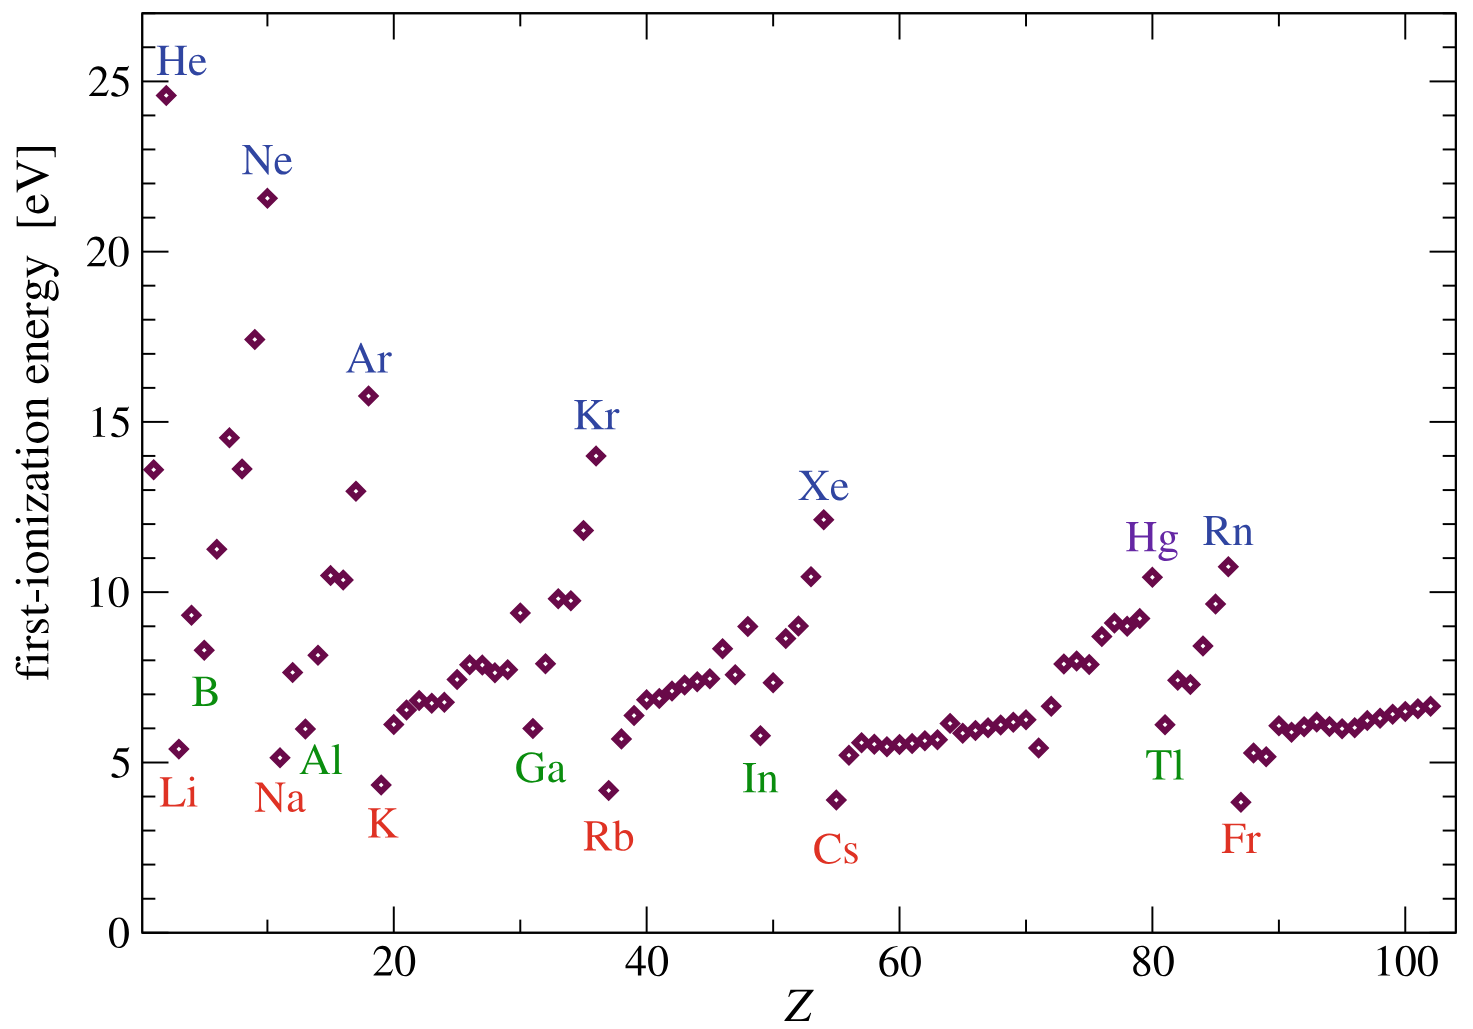
\includegraphics[width = 0.49 \textwidth]{ionization-energy.png}
	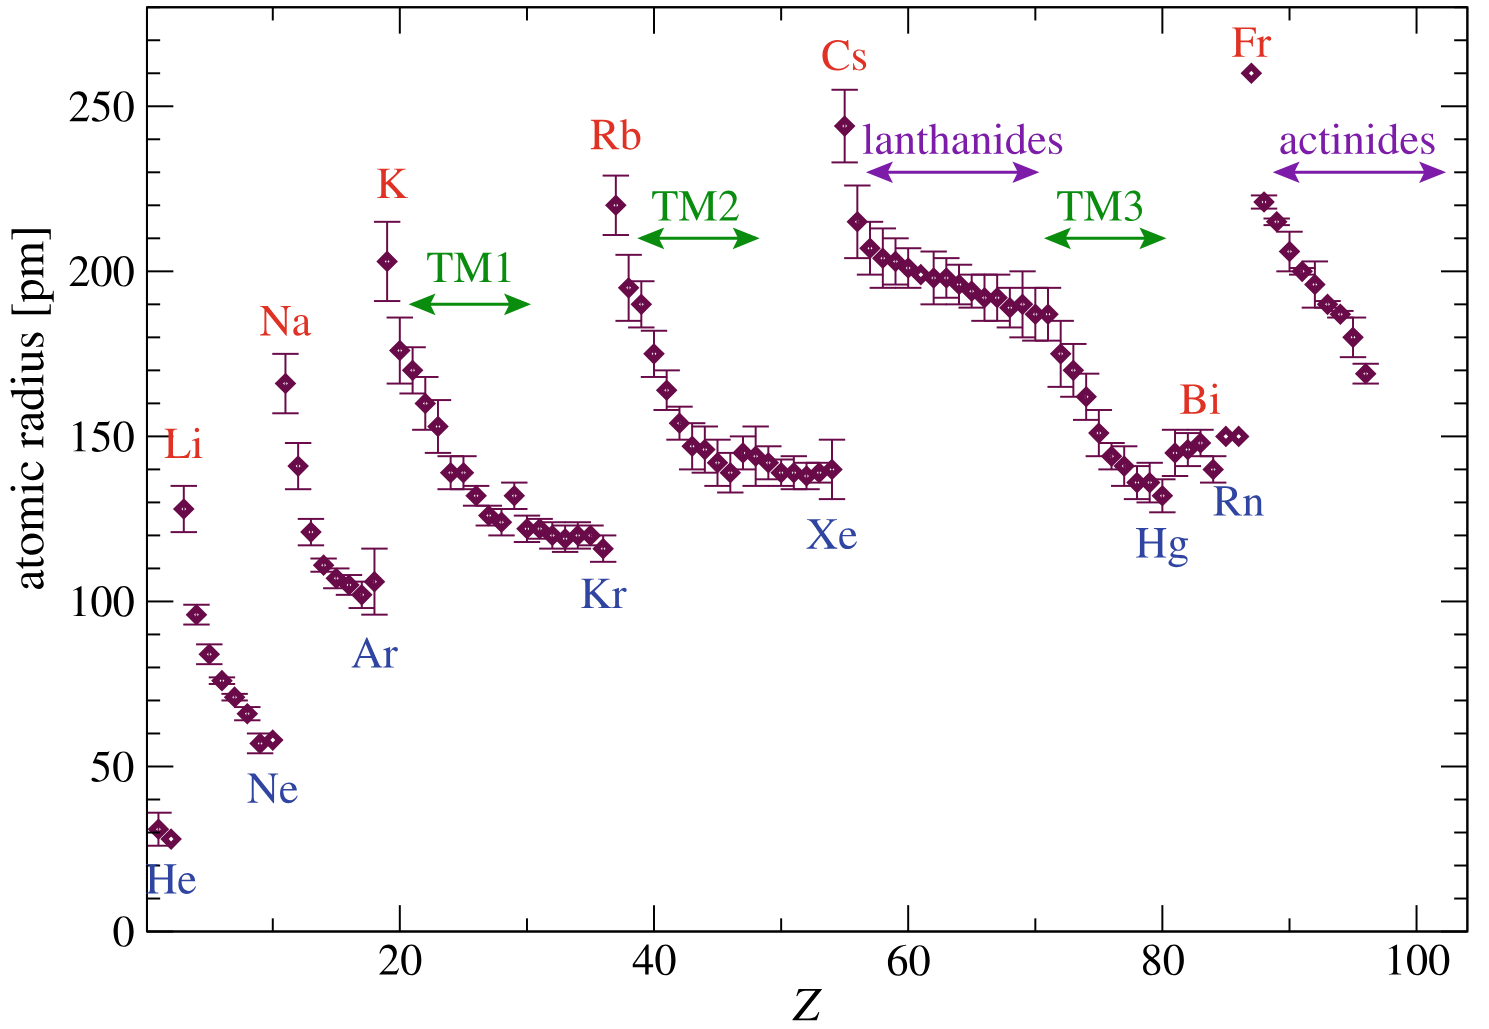
\includegraphics[width = 0.49 \textwidth]{atomic-radius.png}
	\caption{First ionization energy and atomic radius across the periodic table.}
	\label{ion-en-atom-rad}
\end{figure}

Come si può vedere in Fig. \ref{ion-en-atom-rad}, sperimentalmente viene confermato il fatto che i gas nobili hanno shell di valenza complete, poiché presentano energia di prima ionizzazione massima e raggio atomico minimo rispetto agli elementi del loro gruppo. Al contrario, i metalli alcalini hanno un solo elettrone di valenza, per di più molto distante dalle shell interne, come si evince da considerazioni analoghe. \\
Si vede inoltre che gli atomi con shell $ \text{d} $ o $ \text{f} $ incomplete tendono ad avere proprietà (a basse energie) piuttosto uniformi: vengono perciò ragguppati in metalli di transizione ($ \text{3d} $, $ \text{4d} $ e $ \text{5d} $), lantanidi ($ \text{4f} $) ed attinidi ($ \text{5f} $).

\begin{example}{Energia di prima ionizzazione dell'elio}{}
	Se si considera l'$ \ch{He} $, dallo studio della sua energia di ionizzazione si vede come sia necessario considerare l'interazione tra elettroni. Mentre l'energia del catione $ \ch{He}^+ $ è calcolabile usando lo spettro idrogenoide (Eq. \ref{eq:1-e-en}), trovando $ E(\ch{He}^+) = -54\ev $, se si usasse quest'ultimo per calcolare anche l'energia di $ \ch{He} $ si troverebbe $ E(\ch{He}) = 2 E(\ch{He}^+) = - 108\ev $, per un'energia di prima ionizzazione $ E_1(\ch{He}) = 54\ev $ in contrasto col dato sperimentale $ E_1(\ch{He}^+) \simeq 24\ev $. Tenendo conto dell'interazione elettronica, ovvero della correzione in Sec. \ref{he-inter-electr}, si trova $ E(\ch{He}) = -77.8\ev $, ovvero $ E_1(\ch{He}) = 24.2\ev $, dunque in perfetto accordo con le osservazioni.
\end{example}

\subsubsection{Regole di Hund}

Per ottenere la configurazione elettronica del ground state (o degli stati eccitati) di un atomo è necessario svolgere la trattazione HF completa. È però possibile approssimare il risultato utilizzando delle regole semi-empiriche, dette regole di Hund, per stabilire quale, tra tutti gli stati possibili\footnotemark, è il ground state; in ordine di importanza:
\begin{enumerate}
	\item massimizzare lo spin totale $ \bs{S} $;
	\item massimizzare il momento angolare orbitale totale $ \bs{L} $;
	\item per il momento angolare totale $ \bs{J} $, in base al riempimento della shell:
		\begin{itemize}
			\item se è meno di semipiena, minimizzare $ \bs{J} $;
			\item se è più di semipiena, massimizzare $ \bs{J} $.
		\end{itemize}
\end{enumerate}
Queste regole si basano sul minimizzare l'energia del sistema. Per quanto riguarda la prima regola, gli stati atomici a spin più basso hanno energia maggiore poiché, essendo il moto degli elettroni poco correlato, questi tendono a trovarsi in media vicini gli uni agli altri più spesso rispetto agli stati atomici a spin più alto, risultando in una maggiore energia Coulombiana. \\
La seconda regola, invece, deriva dal fatto che, a parità di spin, gli elettroni si evitano più efficientemente quando ruotano in maniera coordinata, ovvero in stati atomici ad alto momento angolare orbitale (a parità di spin, massimizzato dalla prima regola). \\
Infine, massimizzati $ \bs{S} $ ed $ \bs{L} $, rimane da determinare $ \bs{J} $ (poiché $ \bs{S} $ ed $ \bs{L} $ vengono accoppiati dall'interazione spin-orbita): lo stato ad energia minore viene determianto dal segno del coefficiente spin-orbita. Se si considera una shell meno che semipiena, questo sarà naturalmente positivo, ma, se si considera una shell più che semipiena, gli elettroni mancanti possono essere interpretati come particelle di carica opposta, così da avere:
\begin{equation*}
	\mathcal{H}_\text{s-o} = \xi_{n,\ell} \sum_{i = 1}^{n_e} \bs{s}_i \cdot \bs{\ell}_i = \xi_{n,\ell} \underbrace{\sum_{i = 1}^{t} \bs{s}_i \cdot \bs{\ell}_i}_{0} - \xi_{n,\ell} \sum_{i = n_e+1}^{t} \bs{s}_i \cdot \bs{\ell}_i = - \xi_{n,\ell} \sum_{i = n_e + 1}^{t} \bs{s}_i \cdot \bs{\ell}_i
\end{equation*}
Dunque, si vede che nelle shell meno che semipiene va minimizzato $ \bs{J} $, mentre in quelle più che semipiene esso va massimizzato. \\
Si noti che queste regole hanno natura fenomenologica e, sebbene risultino alquanto accurate nel predire i ground states atomici, risultano molto spesso fallaci nella trattazione degli stati eccitati.

\footnotetext{In questo caso, si considerano solo i microstati associati all'ultima shell non completamente riempita: detti $ t $ il numero massimo di elettroni allocabili in tale shell ed $ n_e $ il numero di elettroni da collocarvi, il numero totale di microstati possibili è $ \binom{t}{n_e} $.}

\paragraph{Coupling schemes}

Le regole di Hund si basano sul cosiddetto \textit{Russell-Saunders coupling}, il quale prevede che vengano prima vengano accoppiati i vari $ \bs{s}_i $ a dare $ \bs{S} $ ed i vari $ \bs{\ell}_i $ a dare $ \bs{L} $, e successivamente $ \bs{S} $ ed $ \bs{L} $ vengano accoppiati a dare $ \bs{J} $. Questo coupling scheme risulta efficacie in atomi a basso $ Z $, in cui il potenziale HF (Coulombiano + scambio) è dominante rispetto a quello spin-orbita. \\
Al contrario, per atomi con $ Z \ge 50 $ il potenziale spin-orbita diventa dominante\footnotemark: in questo caso, è necessario prima accoppiare i vari $ \bs{s}_i $ e $ \bs{\ell}_i $, ottenendo i $ \bs{j}_i $ individuali, e poi accoppiare quest'ultimi per ottenere $ \bs{J} $. Questo è noto come \textit{jj coupling}. \\
Mentre la base LS è quasi-diagonale per basso $ Z $ e quella jj lo è per alto $ Z $, a $ Z $ intermedi è necessario diagonalizzare opportunamente sia il termine Coulombiano che quello di spin-orbita.

\footnotetext{Mentre l'energia d'interazione spin-orbita cresce all'aumentare di $ Z $, l'energia d'interazione Coulombiana rimane pressoché costante, risultando addirittura attenuata dal progressivo allontanamento degli elettroni di valenza dal nucleo.}

\section{Spettroscopia}

\subsection{Transizioni di dipolo elettrico}

Nel caso di un sistema ad $ N $ elettroni, l'operatore dipolo elettrico è definito come la somma degli operatori single-particle:
\begin{equation}
	\ve{d} \defeq \sum_{i = 1}^{N} \ve{d}_i = - q_e \sum_{i = 1}^{N} \ve{r}_i
\end{equation}

\begin{proposition}{Transizioni di dipolo elettrico}{}
	Nei sistemi ad $ N $ elettroni, le transizioni di dipolo elettrico sono realizzate da un \textit{singolo elettrone} che transiziona, mentre gli altri rimangono nello stato single-particle iniziale.

	\tcblower

	\begin{proof}
		Nell'approssimazione HF di campo medio:
		\begin{equation*}
			\begin{split}
				& {^\text{(a)}\langle} \beta_1, \dots, \beta_N | \sum_{i = 1}^{N} \ve{d}_i | \alpha_1, \dots, \alpha_N {\rangle^\text{(a)}} = \\
				& \qquad \qquad \qquad = \frac{1}{N!} \sum_{i = 1}^{N} \sum_{\pi,\rho \in S^N} (-1)^{\{\pi\} + \{\rho\}} \braket{\beta_{\pi(1)} | \alpha_{\rho(1)}} \dots \braket{\beta_{\pi(i)} | \ve{d}_i | \alpha_{\rho(i)}} \dots \braket{\beta_{\pi(N)} | \alpha_{\rho(N)}} \\
				& \qquad \qquad \qquad = \frac{1}{N!} \sum_{i = 1}^{N} \sum_{\pi,\rho \in S^N} (-1)^{\{\pi\} + \{\rho\}} \braket{\beta_{\pi(i)} | \ve{d}_i | \alpha_{\rho(i)}} \prod_{j \neq i} \delta_{\beta_{\pi(j)} , \alpha_{\rho(j)}}
			\end{split}
		\end{equation*}
		Si noti che queste $ N - 1 $ delta di Kronecker fissano completamente la permutazione $ \rho \equiv \pi $, dunque:
		\begin{equation*}
			\begin{split}
				{^\text{(a)}\langle} \beta_1, \dots, \beta_N | \sum_{i = 1}^{N} \ve{d}_i | \alpha_1, \dots, \alpha_N {\rangle^\text{(a)}}
				& = \frac{1}{N!} \sum_{i = 1}^{N} \sum_{\pi \in S^N} \braket{\beta_{\pi(i)} | \ve{d}_i | \alpha_{\pi(i)}} \prod_{i \neq j} \delta_{\beta_{\pi(j)} , \alpha_{\pi(j)}} \\
				& = \sum_{i = 1}^{N} \braket{\beta_i | \ve{d}_i | \alpha_i} \prod_{j \neq i} \delta_{\beta_j , \alpha_j}
			\end{split}
		\end{equation*}
		Ciò equivale alla tesi.
	\end{proof}
\end{proposition}

Dato che le transizioni di dipolo-elettrico di un sistema ad $ N $ elettroni si riducono a quelle single-particle, si ha che le transizioni ammesse sono quelle in cui la configurazione elettronica dell'atomo cambia per un solo elettrone, tale per cui $ \Delta \ell_i = \pm 1 $ (più le altre condizioni in Eq. \ref{eq:1-e-el-dip-tr-m}-\ref{eq:1-e-el-dip-tr-spin}).

\begin{example}{Transizioni di dipolo elettrico del berillio}{}
	La configurazione elettronica del ground state del berillio è $ [\ch{Be}] = \text{1s}^2 \text{2s}^2 $. Possibili transizioni di dipolo elettrico ammesse sono $ \text{1s}^2 \text{2s}^2 \rightarrow \text{1s}^2 \text{2s}^1 \text{2p}^1 $ o $ \text{1s}^1 \text{2s}^2 \text{2p}^1 \rightarrow \text{1s}^1 \text{2s}^2 \text{4d}^1 $; transizioni proibite sono invece $ \text{1s}^2 \text{2s}^2 \rightarrow \text{1s}^2 \text{2s}^1 \text{3d}^1 $ o $ \text{1s}^2 \text{2s}^2 \rightarrow \text{1s}^1 \text{2s}^1 \text{2p}^1 \text{3p}^1 $.
\end{example}

\subsection{Eccitazioni di core}

Secondo la teoria HF, gli stati di core (single-particle), ovvero tutti gli elettroni non di valenza, subiscono una schermatura del potenziale del nucleo trascurabile, dunque la loro energia è molto negativa ($ \propto - Z^2 $): ciò è confermato dal fatto che, se per esempio si considera un eccitazione del $ \ch{Na} $ del tipo $ \text{1s}^2 \text{2s}^2 \text{2p}^6 \text{3s}^1 \rightarrow \text{1s}^1 \text{2s}^2 \text{2p}^6 \text{3s}^2 $, sono necessarie energie dell'ordine $ \sim 1\kev $ per eccitare gli stati di core al primo stato eccitato disponibile (a causa del principio d'esclusione). \\
Ne consegue che, data la dipendenza del decay rate da $ E_\text{if}^3 $, le eccitazioni di core presentano delle linee spettrali estremamente allargate, oltre $ \hbar \gamma \sim 1\ev $. Inoltre, dall'Eq. \ref{eq:electric-dipole-decay-rate}, si vede che $ \gamma \sim Z^4 $.

\begin{figure}
	\centering
	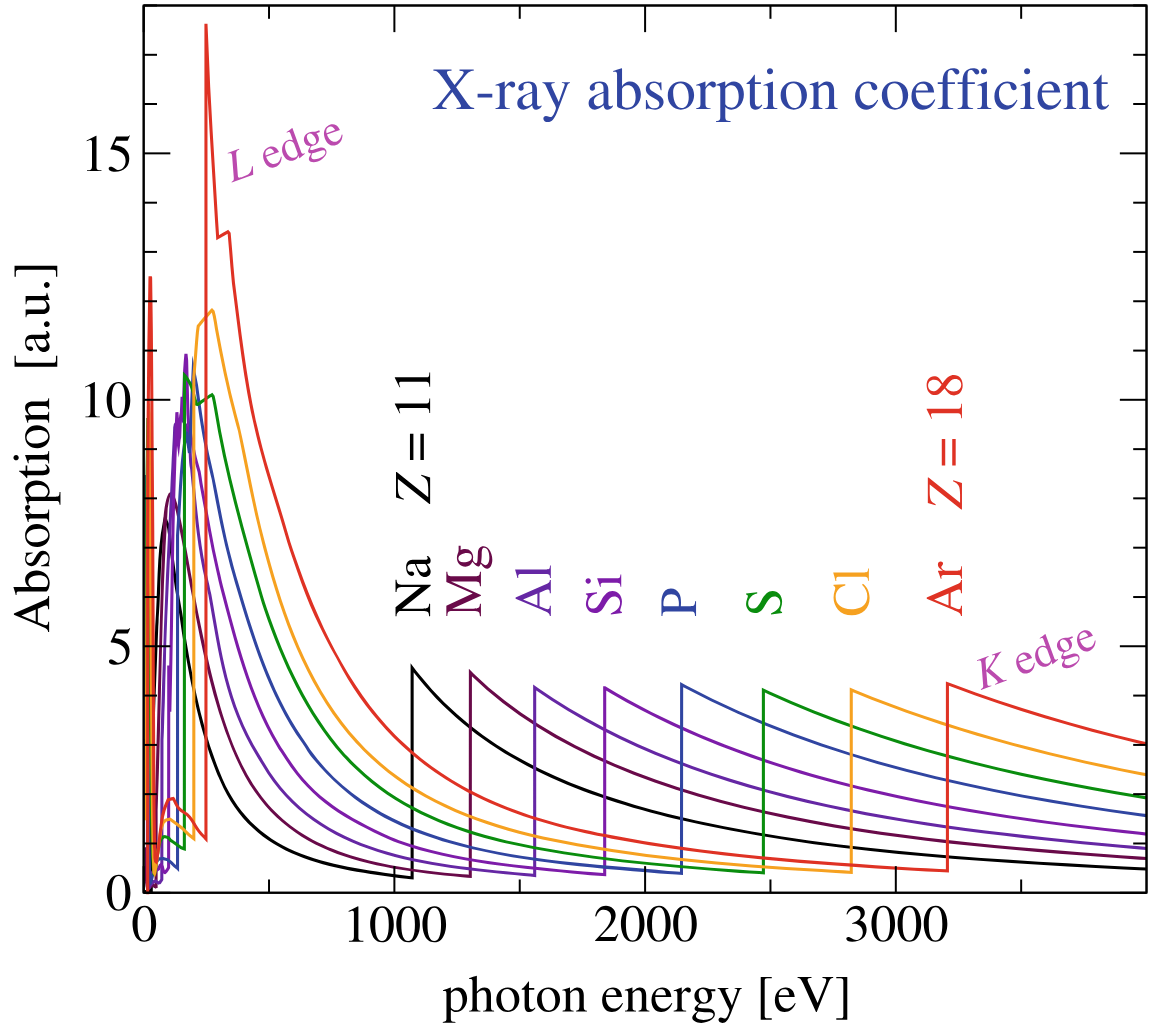
\includegraphics[width = 0.45 \textwidth]{core-exc-x-rays.png}
	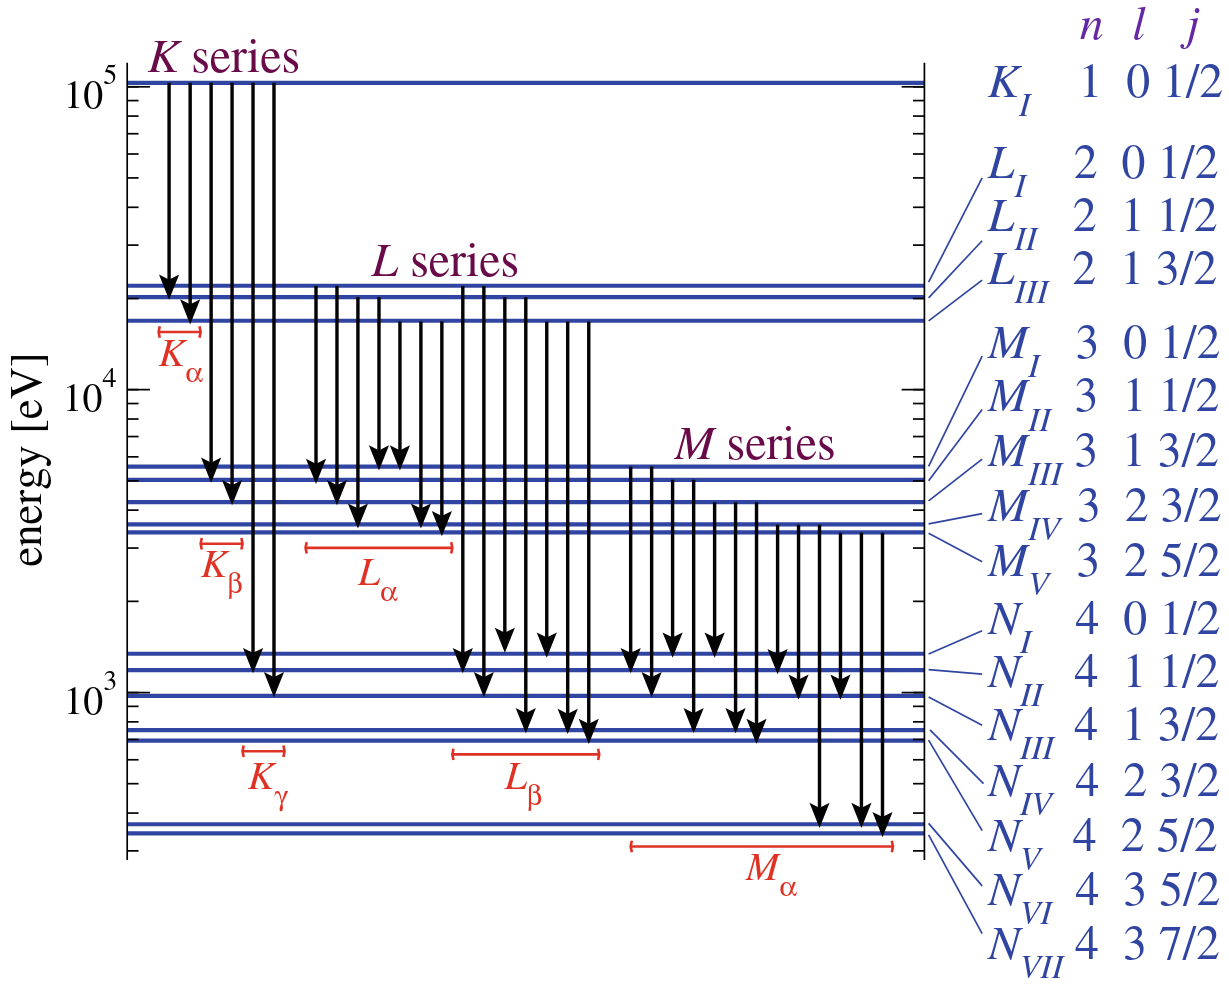
\includegraphics[width = 0.45 \textwidth]{core-exc-spectr.png}
	\caption{Observed X-ray absorption for third-period elements and observed core-level structure of $ \ch{U} $.}
	\label{core-exc}
\end{figure}

Le eccitazioni di core sono molto studiate a livello sperimentale: as esempio, i dati relativi all'assorbimento di raggi X (Fig. \ref{core-exc}) mostrano una certa regolarità per $ E_\gamma > 50\ev $, con un andamento sistematico rispetto a $ Z $. In particolare, si vede che negli spettri d'assorbimento di raggi X i picchi hanno una forma asimmetrica: per quanto riguarda l'estremità energeticamente inferiore, non può avvenire alcun assorbimento, in quanto l'energia non sarebbe sufficiente ad eccitare l'elettrone di core al primo stato eccitato libero (e, per il principio d'esclusione, esso non può essere eccitato a nessuno stato al di sotto di questo); superata la soglia d'assorbimento, invece, l'elettrone può essere eccitato a vari stati non-occupati, sia legati che non, risultando in uno spettro d'assorbimento continuo. \\
Si noti, inoltre, che all'aumentare dell'energia del fotone assorbito aumenta anche l'energia cinetica dell'elettrone ($ K_e = E_\gamma - E_\text{exc} $): conseguentemente, lo stato eccitato finale diventa progressivamente più ortogonale a quello iniziale. Ciò determina una rapida diminuzione di $ \gamma_\text{if} \propto \braket{\text{i} | \ve{d} | \text{f}} $, ovvero un rallentamento del decadimento. Per lo stesso motivo, inoltre, si capisce perché l'assorbimento di raggi X genera eccitazioni di core: se il fotone fosse assorbito da un elettrone di valenza, il quale è debolmente legato, la sua energia cinetica sarebbe molto alta, rendendo lo stato eccitato molto ortogonale rispetto a quello iniziale e rendendo $ \gamma $ trascurabile.

\subsubsection{Legge di Moseley}

Per quanto riguarda le transizioni tra stati di core, si adotta la seguente notazione: un \textit{hole} (elettrone mancante) in una shell $ n = 1,2,3,4,\dots$ è indicato da $ K,L,M,N,\dots $, mentre il numero di salti di shell è indicato da $ \alpha,\beta,\gamma,\dots$.

\begin{example}{Transizioni di core}{}
	Una transizione del tipo $ \text{1s}^1 \text{2s}^2 \text{2p}^6 \dots \rightarrow \text{1s}^2 \text{2s}^2 \text{2p}^5 \dots $ è indicata come $ K_\alpha \equiv K \rightarrow L $. Una transizione del tipo $ \text{1s}^2 \text{2s}^2 \text{2p}^5 \text{3s}^2 \text{3p}^6 \text{4s}^2 \dots \rightarrow \text{1s}^2 \text{2s}^2 \text{2p}^6 \text{3s}^2 \text{3p}^6 \text{4s}^1 \dots $ è $ L_\beta \equiv L \rightarrow N $.
\end{example}

Per quanto riguarda le linee spettrali $ K_\alpha $, dai dati sperimentali si evince una legge fenomenologica, detta \textit{legge di Moseley}:
\begin{equation}
	\frac{1}{\lambda_{K_\alpha}} \approx C \left( Z - a \right)^2
\end{equation}
dove $ C \approx \frac{3}{8} \frac{E_\text{Ha}}{2\pi \hbar c} \simeq 8.25 \cdot 10^6 \,\text{m}^{-1} $ ed $ a $ è il \textit{parametro di screening}. Quest'ultimo tiene conto dello screening che la carica nucleare subisce a causa degli elettroni di core (vedere Fig. \ref{screening}): non c'è una definizione ben precisa di $ a $, in quanto è un parametro fenomenologico, ma un buon accordo coi dati sperimentali è dato dal numero di elettroni nelle shell più interne a quelle considerate, includendo anche quella in esame (dunque $ (n,a) = (1,2) , (2,10), (3,28), \dots $).

\begin{figure}
	\centering
	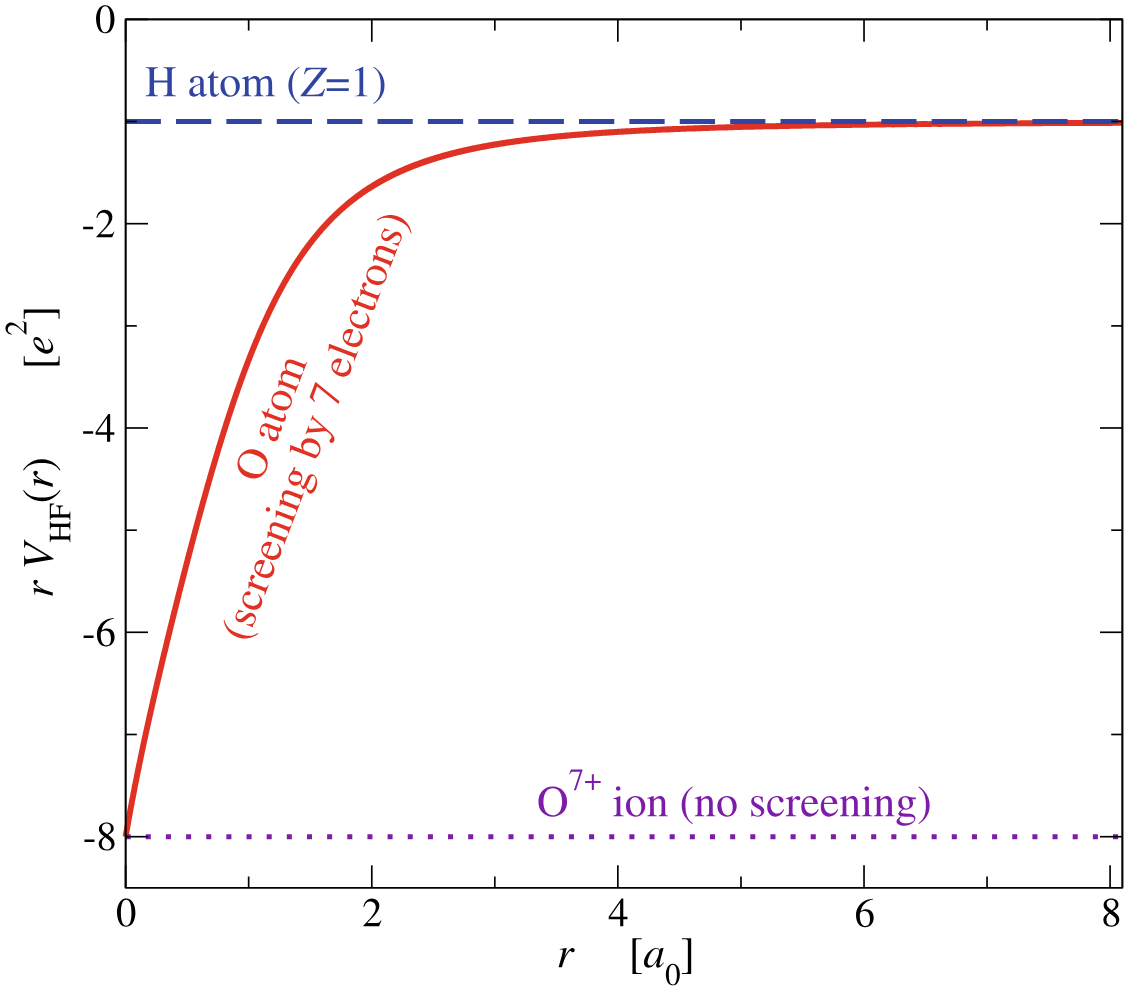
\includegraphics[width = 0.50 \textwidth]{screening.png}
	\caption{HF effective potential for atomic $ \ch{O} $ ($ N = Z = 8 $).}
	\label{screening}
\end{figure}

\subsection{Campo magnetico esterno}

Quando viene applicato un campo magnetico ad un MAE, si osserva un comportamento diverso in base alla presenza o meno di un momento magnetico. \\
Se si considera un atomo con $ J = 0 $, esso non ha alcun momento magnetico permanente: il campo esterno induce un piccolo momento magnetico $ \mu \sim \mu_\text{B} \frac{\mu_\text{B} B}{\Delta} $, dove $ \Delta $ è la differenza energetica tra il ground state ed il primo stato eccitato con $ J \neq 0 $, ma questi effetti sono trascurabili. \\
Al contrario, atomi con $ J \neq 0 $ hanno un momento magnetico permanente:
\begin{equation}
	\bs{\mu} = - g_J \mu_\text{B} \bs{J}
\end{equation}
dove $ g_J $ è il fattore di Landé (Eq. \ref{eq:lande-g-factor} con $ S,L,J $, nel LS coupling). Questo momento mangetico è rilevante nel limite Zeeman di campo esterno debole, che nella pratica è quello più importante in quanto difficilmente in laboratorio di riescono a produrre campi magnetici tali da dominare sull'interazione spin-orbita. \\
Per quanto riguarda lo splitting delle linee spettrali, si distingue tra \textit{regular Zeeman splitting}, nel caso in cui esse vengano splittate regolamente in $ 2J + 1 $ linee spettrali (quando i fattori di Landé dello stato iniziale e finale sono uguali), e \textit{anomalous Zeeman splitting}, nel caso in cui lo splitting pattern sia più complesso (quando i fattori di Landé dello stato iniziale e finale sono diversi). \\
Un'importante strumento sperimentale per studiare la degenerazione dei ground states dei MAE è l'apparato di Stern-Gerlach, nel quale gli atomi vengono deflessi (Eq. \ref{eq:stern-gerlach}) secondo:
\begin{equation*}
	F_z = \mu_z \frac{\pa B_z}{\pa z} = - g_J \mu_\text{B} M_J \frac{\pa B_z}{\pa z}
\end{equation*}
Il numero di sotto-fasci in cui viene splittato il fascio iniziale dà dunque una misura diretta dei possibili valori di $ M_J $, ovvero della degenerazione $ 2J + 1 $ del ground state.












\chapter{Molecole}
\selectlanguage{italian}

Lo studio delle molecole, ed in particolare delle molecole diatomiche, permette d'illustrare due concetti fondamentali nello studio della fisica della materia: la separazione adiabatica del moto elettronico da quello nucleare ed il legame chimico.

\section{Separazione adiabatica}

L'Hamiltoniana per un sistema generico di $ M $ nuclei ed $ N $ elettroni è:
\begin{equation}
	\mathcal{H} = T_n + T_e + V_{ne} + V_{nn} + V_{ee}
	\label{eq:mol-ham-tot}
\end{equation}
Sebbene la funzione d'onda totale del sistema $ \Psi(r,R) $ dipenda dalle coordinate $ r $ di tutti gli elettroni ed $ R $ di tutti i nuclei, è possibile semplificare il problema. Infatti, essendo le masse dei nuclei e quelle degli elettroni diverse di circa tre ordini di grandezza, si può considerare che anche le time-scales dei moti dei nuclei siano tre ordini di grandezza maggiori rispetto a quelle dei moti degli elettroni: c'è dunque un disaccoppiamento dei due moti\footnotemark, in quanto si può assumere che il moto nucleare non induca alcuna transizione sugli stati elettronici (poiché le energie dei moti nucleari sono troppo piccole per colmare i gap energetici tra stati elettronici), da cui il nome di \textit{separazione adiabatica} (o di Born-Oppenheimer).

\footnotetext{In maniera approssimativa, si può dire che gli elettroni percepiscono i nuclei come fermi, mentre i nuclei risentono solo degli effetti medi del moto elettronico.}

\begin{definition}{Fattorizzazione adiabatica}{}
	La funzione d'onda totale del sistema si fattorizza come:
	\begin{equation}
		\Psi(r,R) = \Phi(R) \psi_e(r,R)
	\end{equation}
	dove $ \Phi(R) $ è la \textit{funzione d'onda nucleare} e $ \psi_e(r,R) $ è la \textit{funzione d'onda elettronica}, la quale è soluzione dell'equazione d'onda elettronica:
	\begin{equation}
		[T_e + V_{ne}(r,R) + V_{ee}(r)] \psi_e^{(a)}(r,R) = E_e^{(a)}(R) \psi_e^{(a)}(r,R)
		\label{eq:mol-el-eq}
	\end{equation}
	con $ (a) $ set di autovalori.
\end{definition}

La funzione d'onda $ \psi_e^{(a)}(r,R) $ descrive un autostato elettronico per una geometria fissata dei nuclei: la dipendenza da $ R $ di $ \psi_e^{(a)}(r,R) $ ed $ E_e^{(a)}(R) $ è puramente parametrica.

\begin{proposition}{Equazione d'onda nucleare}{}
	La funzione d'onda nucleare $ \Phi(R) $ è soluzione dell'equazione d'onda nucleare:
	\begin{equation}
		[T_n + V_\text{ad}^{(a)}(R)] \Phi(R) = E_\text{tot} \Phi(R)
		\label{eq:mol-nucl-eq}
	\end{equation}
	dove il \textit{potenziale adiabatico totale} è:
	\begin{equation}
		V_\text{ad}^{(a)}(R) \equiv E_e^{(a)}(R) + V_{nn}(R)
		\label{eq:ad-pot}
	\end{equation}

	\tcblower

	\begin{proof}
		Partendo dall'Eq. \ref{eq:mol-ham-tot}:
		\begin{equation*}
			[T_n + T_e + V_{nn} + V_{ne} + V_{ee}] \Phi(R) \psi_e(r,R) = E_\text{tot} \Phi(R) \psi_e(r,R)
		\end{equation*}
		e notando che, essendo $ T_e \sim \lap_r $, si ha $ T_e [\Phi(R) \psi_e(r,R)] = \Phi(R) T_e \psi_e(r,R) $:
		\begin{equation*}
			- \sum_\alpha \frac{\hbar^2}{2M_\alpha} \lap_{R_\alpha} [\Phi(R) \psi_e(r,R)] + \Phi(R) \underbrace{[T_e + V_{nn} + V_{ne}] \psi_e(r,R)}_{\text{equazione elettronica}} + \Phi(R) V_{nn} \psi_e(r,R) = E_\text{tot} \Psi(r,R)
		\end{equation*}
		Il primo termine diventa:
		\begin{equation*}
			\begin{split}
				- \sum_\alpha \frac{\hbar^2}{2m_\alpha} \lap_{R_\alpha} [\Phi(R) \psi_e(r,R)]
				= & - \sum_\alpha \frac{\hbar^2}{2M_\alpha} [\Phi(R) \lap_{R_\alpha} \psi_e(r,R) + 2 \nabla_{R_\alpha} \Phi(R) \cdot \nabla_{R_\alpha} \psi_e(r,R)] \\
				& - \psi_e(r,R) \sum_\alpha \frac{\hbar^2}{2M_\alpha} \lap_{R_\alpha} \Phi(R)
			\end{split}
		\end{equation*}
		I primi due termini (non-adiabatici) possono essere ignorati in approssimazione adiabatica, così da rimanere solo col terzo:
		\begin{equation*}
			\psi_e^{(a)}(r,R) [T_n + E_e^{(a)}(R) + V_{nn}(R)] \Phi(R) = E_\text{tot} \Phi(R) \psi_e^{(a)}(r,R)
		\end{equation*}
		Moltiplicando per $ [\psi_e^{(a)}(r,R)]^* $ da sinistra ed integrando su tutte le $ r $ si ottiene infine la tesi.
	\end{proof}
\end{proposition}

L'equazione elettronica presenta, nel caso $ N > 1 $, le stesse complicazioni della trattazione dei MEAs, ed è ugualmente risolvibile col metodo HF (con l'ulteriore complicazione che ora bisogna considerare varie geometrie molecolari date dalle $ R $): una volta selezionato lo stato elettronico $ a $, esso segue adiabaticamente il moto nucleare, non transizionando ad altri stati $ a' \neq a $ (questa è un'approssimazione della realtà). \\
Per quanto riguarda l'equazione nucleare, essa esprime il moto dei nuclei all'interno del potenziale adiabatico totale, composto da un termine Coulombiano repulsivo ed un contributo elettronico attrattivo (è ciò che permette alle molecole di esistere come stati legati). $ V_\text{ad}^{(a)}(R) $, funzione di $ 3M $ variabili, presenta una simmetria roto-traslazionale: ciò suggerisce che esso dipenda dalle distanze relative tra i nuclei atomici. Un esempio di andamento di $ V_\text{ad}^{(a)}(R) $ è riportato in Fig. \ref{ad-pot} (per il ground state di una molecola diatomica): si vede che il potenziale ha un minimo $ R_\text{m} $ finito, attorno al quale avvengono le oscillazioni del moto nucleare a bassa temperatura.

\begin{figure}
	\centering
	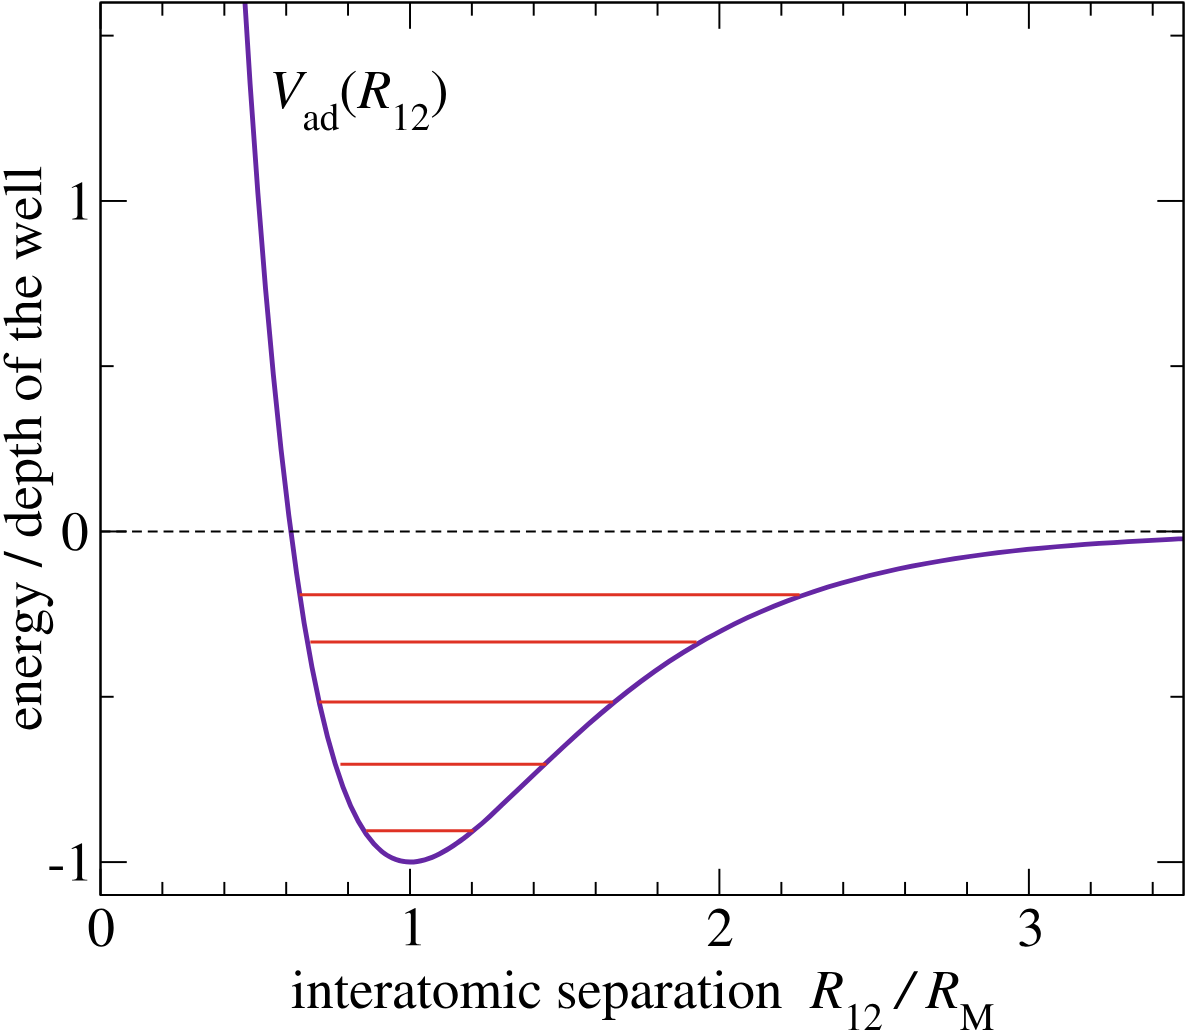
\includegraphics[width = 0.40 \textwidth]{adiabatic-potential.png}
	\caption{Adiabatic potential for a diatomic molecule.}
	\label{ad-pot}
\end{figure}

\section{Legami}

L'andamento del potenziale adiabatico in Fig. \ref{ad-pot} è alquanto generale, anche per molecole con $ M > 2 $, e pone le basi per lo studio di strutture molecolari complesse.

\subsection{\texorpdfstring{$ \ch{H_2^+} $}{H2+}}

Si consideri ad esempio la più semplice molecola diatomica: $ \ch{H_2^+} $. In questo caso non è presente alcuna repulsione elettrone-elettrone, dunque sull'unico elettrone agisce esclusivamente $ V_{ne} = V_\text{L} + V_\text{R} $, dove $ \text{L},\text{R} $ si riferiscono rispettivamente al nucleo sinistro o destro (arbitrariamente scelto il verso dell'asse molecolare $ \hat{\ve{e}}_z $): questi possono essere assunti fissi e posti a $ \pm R_{12}/2 $ lungo $ \hat{\ve{e}}_z $, dove $ \ve{R}_{12} \equiv \abs{\ve{R}_\text{L} - \ve{R}_\text{R}} $.

\begin{figure}[!b]
	\centering
	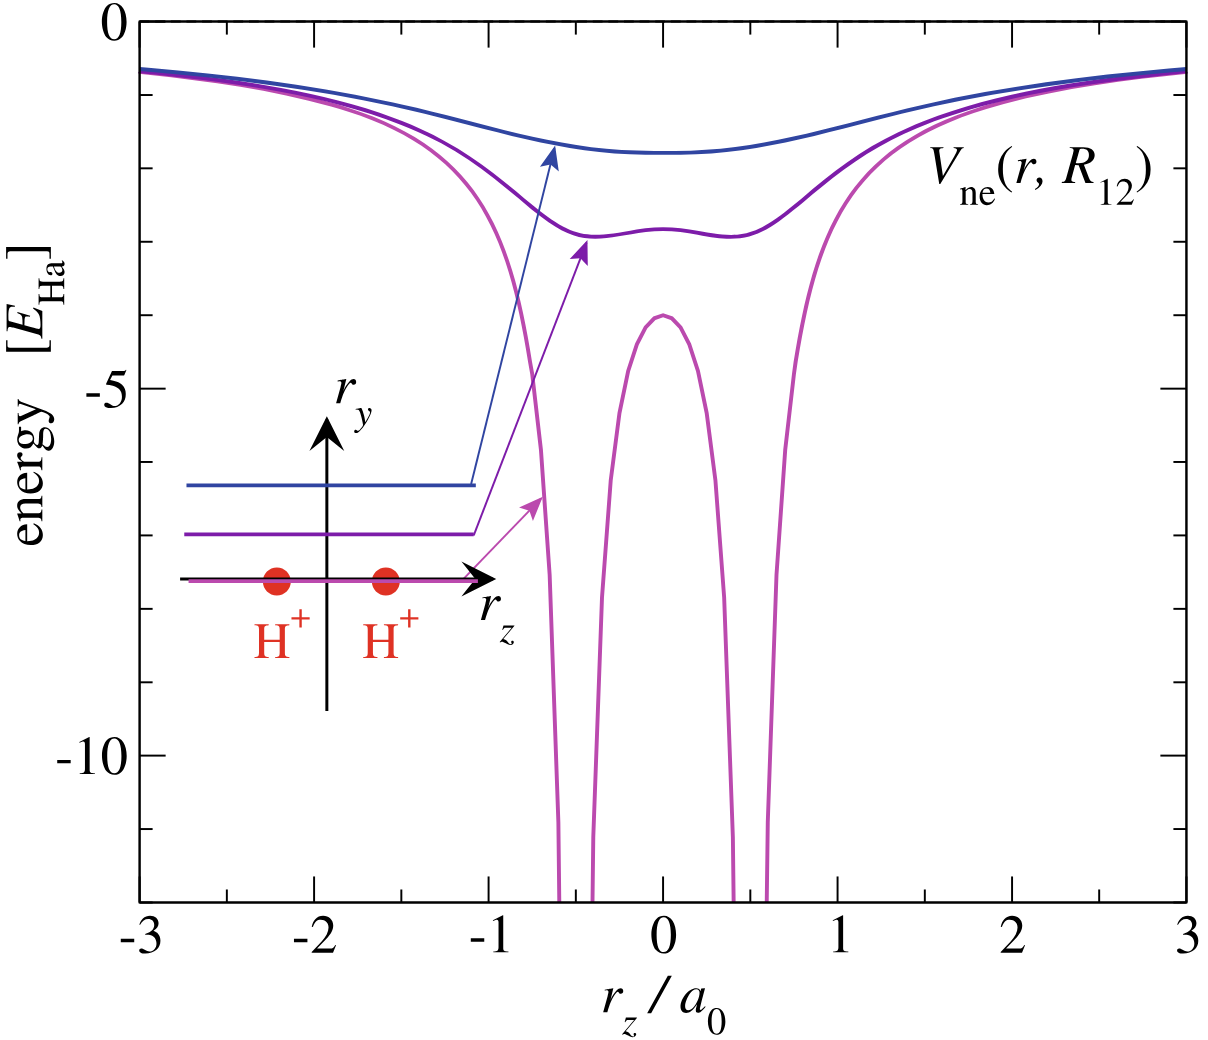
\includegraphics[width = 0.40 \textwidth]{ne-potential-h2.png}
	\caption{$ V_{ne} $ potential for the $ \ch{H_2^^+} $ molecule.}
	\label{ne-h2}
\end{figure}

Con riferimento alla Fig. \ref{ne-h2}, si noti che per $ -R_{12}/2 < r_z < R_{12}/2 $ il potenziale $ V_{ne}(r,R_{12}) $ è circa doppiamente negativo rispetto al caso atomico, suggerendo che l'elettrone potrebbe abbassare la propria energia potenziale media avendo una distribuzione di probabilità piccata nel mezzo dei due nuclei. Per verificare se ciò permette la formazione di un legame, bisogna confrontare che $ V_\text{ad}(R_{12}) < V_\text{ad}(\infty) = E_\text{1s} = -\frac{1}{2} E_\text{Ha} $ (poiché in tale limite si hanno praticamente un protone ed un atomo di idrogeno infinitamente separati, e $ \mu/m_e \approx 1 $). A tal fine, si adotta un approccio variazionale per verificare il valore dell'energia tramite la LCAO (Linear Combination of Atomic Orbitals): si considerino i due ground state atomici $ \ket{\text{1s};\text{L}} \equiv \ket{\text{L}} $ e $ \ket{\text{1s};\text{R}} \equiv \ket{\text{R}} $, assumendo $ \braket{\text{L} | \text{R}} > 0 $, e, data la simmetria assiale (cilindrica attorno $ \hat{\ve{e}}_z $) del problema, si considerino le combinazioni lineari opportunamente normalizzate (plottate in Fig. \ref{gs-h2}):
\begin{equation}
	\ket{\text{S}} = [2(1 + \braket{\text{L} | \text{R}})]^{-1/2} (\ket{\text{L}} + \ket{\text{R}})
	\qquad \qquad
	\ket{\text{A}} = [2(1 - \braket{\text{L} | \text{R}})]^{-1/2} (\ket{\text{L}} - \ket{\text{R}})
	\label{eq:h2-kets}
\end{equation}

\begin{figure}[!b]
	\centering
	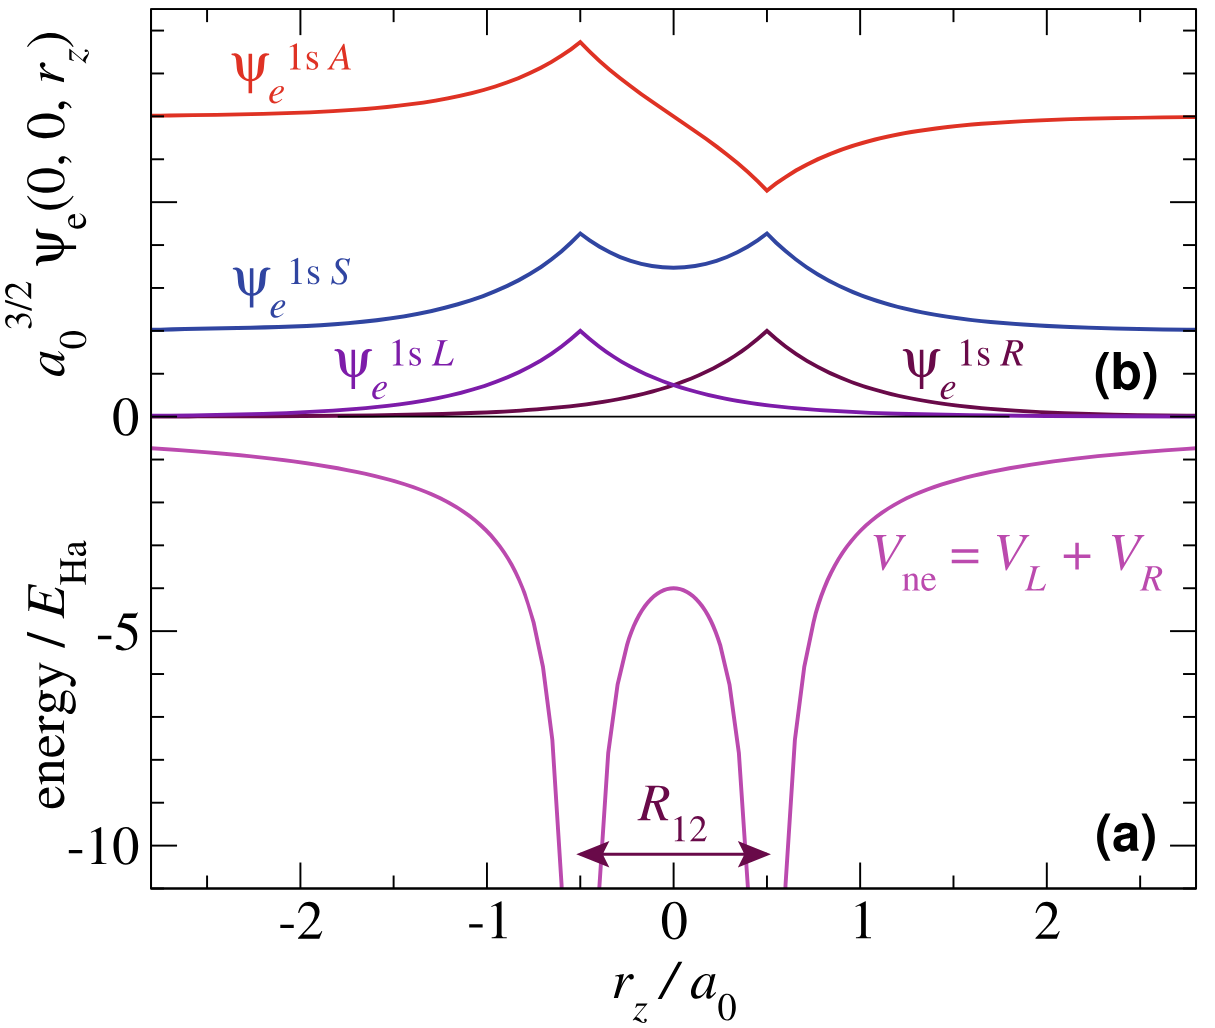
\includegraphics[width = 0.50 \textwidth]{symm-asymm-h2.png}
	\caption{Symmetric and antisymmetric LCAO for the ground state of $ \ch{H_2^+} $.}
	\label{gs-h2}
\end{figure}

Per il principio variazionale, per l'energia del ground state vale $ E_e^{(\text{gs})}(R_{12}) \le \braket{\text{S}/\text{A} | T_e + V_{ne} | \text{S}/\text{A}} \equiv \mathcal{E}_{\text{S},\text{A}} \,\,\forall R_{12} \in \R_+ $.

\begin{proposition}{}{}
	A grande distanza $ R_{12} \gg a_0 $ si ha:
	\begin{equation}
		\mathcal{E}_{\text{S},\text{A}} + \frac{E_\text{Ha}}{2} \simeq - \frac{e^2}{R_{12}} (1 \pm \braket{\text{L} | \text{R}})
		\label{eq:h2-symm-asymm}
	\end{equation}

	\tcblower

	\begin{proof}
		Per calcolo diretto:
		\begin{equation*}
			\begin{split}
				\mathcal{E}_\text{\text{S},\text{A}}
				& = \braket{\text{S}/\text{A} | T_e + V_{ne} | \text{S}/\text{A}} = \frac{\braket{\text{L} | T_e + V_{ne} | \text{L}} \pm \braket{\text{R} | T_e + V_{ne} | \text{L}} + (\text{L} \leftrightarrow \text{R})}{2 (1 \pm \braket{\text{L} | \text{R}})} \\
				& = \frac{\braket{\text{L} | T_e + V_\text{L} | \text{L}} + \braket{\text{L} | V_\text{R} | \text{L}} \pm \braket{\text{R} | T_e + V_\text{L} | \text{L}} \pm \braket{\text{R} | V_\text{R} | \text{L}}}{1 \pm \braket{\text{L} | \text{R}}} = - \frac{E_\text{Ha}}{2} + \frac{\braket{\text{L} | V_\text{R} | \text{L}} \pm \braket{\text{R} | V_\text{R} | \text{L}}}{1 \pm \braket{\text{L} | \text{R}}}
			\end{split}
		\end{equation*}
		essendo $ \ket{\text{L}} $ autostato di $ T_e + V_\text{L} $ con autovalore $ -E_\text{Ha}/2 $. I due elementi di matrice di $ V_\text{R} $ sono entrambi funzioni reali e negative di $ R_{12} $: il termine $ \braket{\text{L} | V_\text{R} | \text{L}} $ rappresenta l'attrazione che il nucleo destro esercita sull'elettrone orbitante attorno al nucleo sinistro, dunque per $ R_{12} $ abbastanza grande si ha:
		\begin{equation*}
			\braket{\text{L} | V_\text{R} | \text{L}} \simeq - \frac{e^2}{R_{12}}
		\end{equation*}
		Il termine $ \braket{\text{R} | V_\text{R} | \text{L}} $, d'altro canto, può essere approssimato considerando che la distribuzione $ \psi_\text{L}(\ve{r}) \psi_\text{R}(\ve{r}) $ è piccata nella regione assiale tra i due nuclei, al centro della quale $ V_\text{R} \simeq - \frac{e^2}{R_{12}/2} $, così che:
		\begin{equation*}
			\braket{\text{R} | V_\text{R} | V_\text{L}} \simeq - \frac{e^2}{R_{12}} 2\braket{\text{L} | \text{R}}
		\end{equation*}
		Si può quindi espandere l'espressione totale considerando $ \braket{\text{L} | \text{R}} $ sufficientemente piccolo:
		\begin{equation*}
			\mathcal{E}_{\text{S},\text{A}} + \frac{E_\text{Ha}}{2} \simeq - \frac{e^2}{R_{12}} \frac{1 \pm 2 \braket{\text{L} | \text{R}}}{1 \pm \braket{\text{L} | \text{R}}} \simeq - \frac{e^2}{R_{12}} (1 \pm \braket{\text{L} | \text{R}})(1 \mp \braket{\text{L} | \text{R}}) \simeq - \frac{e^2}{R_{12}} (1 \pm \braket{\text{L} | \text{R}})
		\end{equation*}
		che è il risultato cercato.
	\end{proof}
\end{proposition}

L'Eq. \ref{eq:h2-symm-asymm} mostra come $ \mathcal{E} + \frac{E_\text{Ha}}{2} + V_{nn} $, con $ V_{nn} = \frac{e^2}{R_{12}} $, sia negativo per $ \ket{\text{S}} $ e positivo per $ \ket{\text{A}} $: ciò significa che la repulsione tra i due nuclei è vinta solo dalla LCAO simmetrica, nel qual caso di forma effettivamente un \textit{legame}. \\
Si può anche considerare il risultato esatto per $ R_{12} $ generico (plottato in Fig. \ref{h2-en}):
\begin{equation}
	\mathcal{E}_{\text{S},\text{A}} = - \frac{E_\text{Ha}}{2} + \frac{\braket{\text{L} | V_\text{R} | \text{L}} \pm \braket{\text{R} | V_\text{R} | \text{L}}}{1 \pm \braket{\text{L} | \text{R}}}
\end{equation}

\begin{figure}[!b]
	\centering
	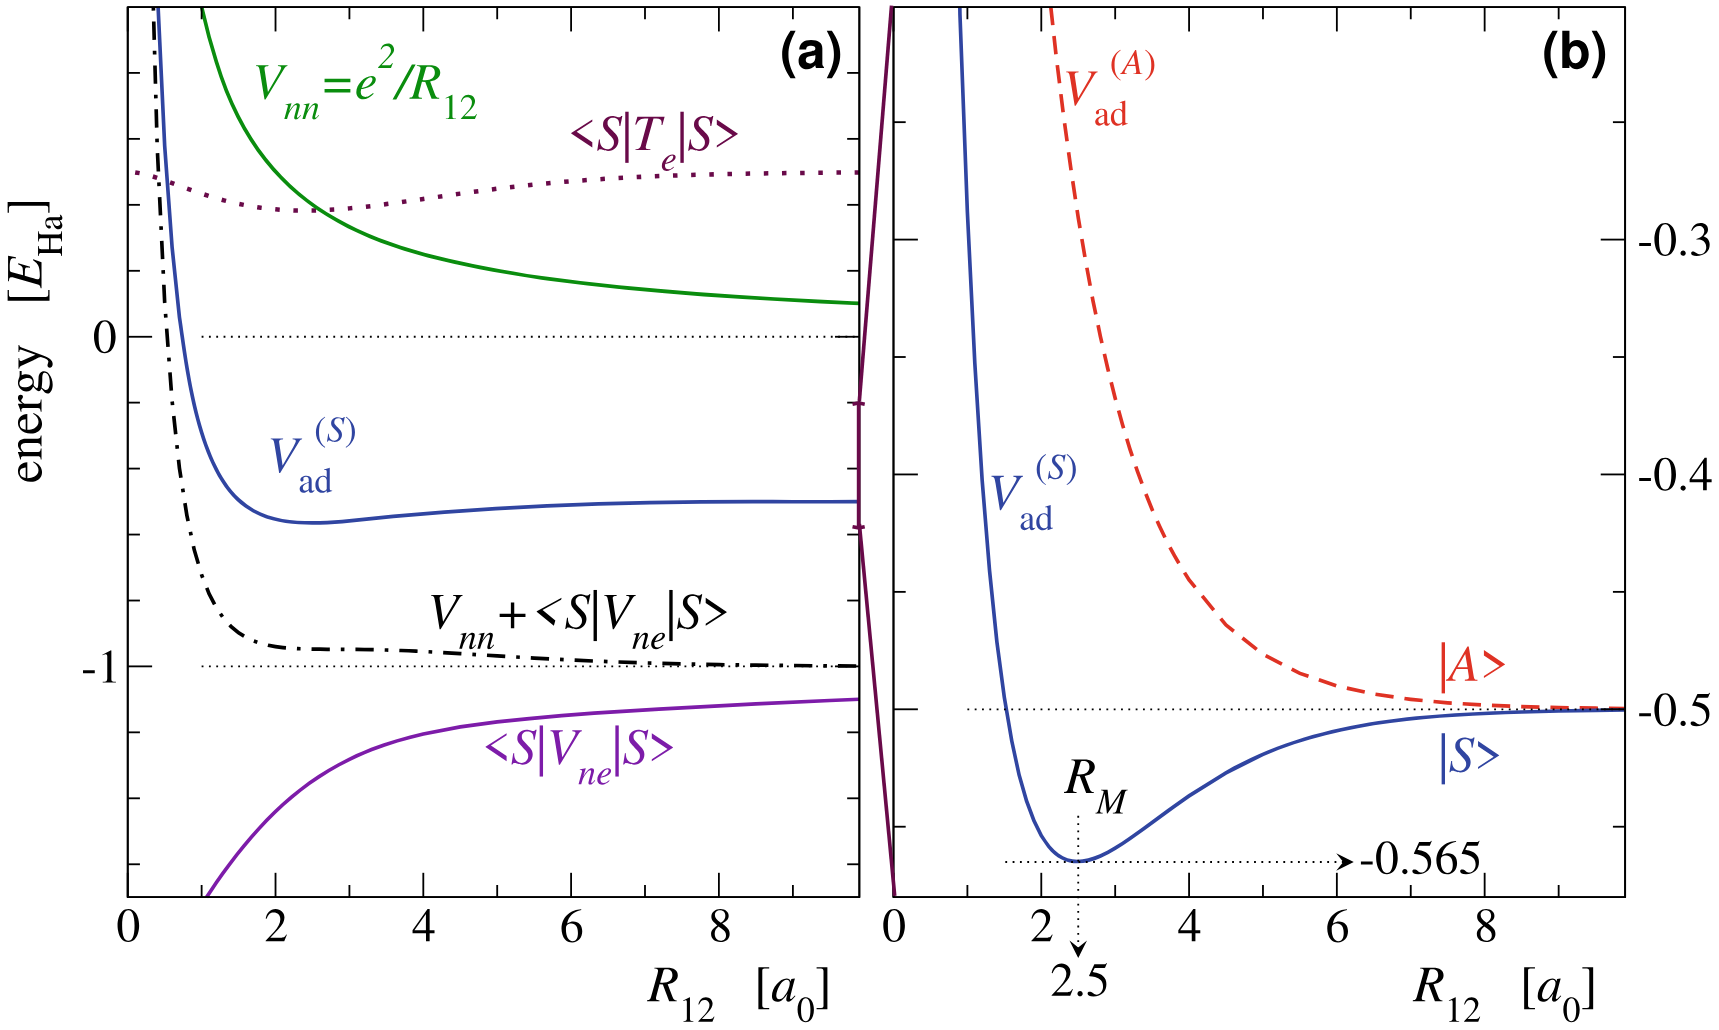
\includegraphics[width = 0.70 \textwidth]{h2-en.png}
	\caption{Total adiabatic potential for $ \ket{\text{S}} $ and $ \ket{\text{A}} $.}
	\label{h2-en}
\end{figure}

Si possono fare alcune osservazioni:
\begin{enumerate}
	\item $ V_\text{ad}^{(\text{S})}(R_{12}) $ presenta un minimo per $ R_{12} = R_\text{m} \simeq 2.5 a_0 $, e questa buca di potenziale è abbastanza profonda da legare i due protoni, pertanto $ \ket{\text{S}} $ è detto \textit{stato legante};
	\item $ V_\text{ad}^{(\text{A})}(R_{12}) $ è monotonamente decrescente, ovvero è un potenziale puramente repulsivo, dunque $ \ket{\text{A}} $ è detto \textit{stato anti-legante};
	\item per $ R_{12} < R_\text{m} $ entrambi i potenziali adiabatici divergono a causa di una singolarità in $ V_{nn} $, il quale non è più efficacemente schermato, ed anche perché gli elettroni sono costretti a muoversi in una buca di potenziale più stretta, dunque con un'energia cinetica maggiore (per il principio d'indeterminazione).
\end{enumerate}
In definitiva, il legame in $ \ch{H_2^+} $ è dovuto sia ad un abbassamento dell'energia cinetica elettronica (poiché l'elettrone si muove in una buca di potenziale più larga) e ad un abbassamento dell'energia potenziale del sistema (poiché l'elettrone scherma la repulsione tra i due nuclei tramite una distribuzione di probabilità piccata nel mezzo). \\
Questo modello variazionale è valido per $ \braket{\text{L} | \text{R}} \ll 1 $, ovvero $ R_{12} \gg a_0 $, ma diventa particolarmente inaccurato per $ R_{12} $ piccolo, poiché in tal caso nella LCAO vanno considerati anche gli stati diversi da $ \text{1s} $: il modello variazionale dà energia di legame molecolare $ V_\text{ad}^{(\text{S})}(\infty) - V_\text{ad}^{(\text{S})}(R_\text{m}) \simeq 1.76\ev $ con $ R_\text{m} = 2.50 a_0 $, mentre il valore sperimentale è $ 2.79\ev $ con $ R_\text{m} = 2.00 a_0 $.

\paragraph{Numeri quantici}

La simmetria di $ \ch{H_2^+} $ è cilindrica, dunque soltanto $ L_z $ può essere diagonalizzato\footnote{In coordinate cilindriche $ \ve{r} = (\rho \cos \varphi, \rho \sin \varphi, z) $ e $ \hat{L}_z \defeq -i\hbar (x \pa_y - y \pa_x) = -i \hbar \pa_\varphi $, quindi le sue autofunzioni sono $ f(\varphi) = \mathcal{N} e^{i m \varphi} $. La condizione di periodicità $ f(\varphi) = f(\varphi + 2\pi) $ impone $ m \in \Z $.}: l'unico numero quantico $ \virgolette{buono} $ è $ m $. In base al valore di $ \abs{m} = 0, 1, 2, \dots $ si indicano gli stati con $ \sigma, \pi, \delta, \dots $; inoltre, gli stati anti-leganti acquistano un asterisco. Si noti che, a parte gli stati $ \sigma $, tutti questi stati sono doppiamente degeneri ($ \pm m $). Questa degenerazione è dovuta a una simmetria dell'Hamiltoniana. In particolare, in assenza di campi magnetici esterni, essa è simmetrica per $ \sigma_\text{v} : \varphi \mapsto -\varphi $, ovvero una riflessione rispetto al piano che contiene l'asse molecolare, la quale implica che l'energia sia $ E = E(\abs{m}) $. Nel caso di molecole diatomiche omonucleari, inoltre, si hanno due ulteriori simmetrie. La prima è la simmetria sotto riflessione rispetto al piano ortogonale all'asse molecolare, denominata $\sigma_\text{n}: z \mapsto -z$, e la seconda è una rotazione di $\pi$: $x \mapsto -x, y \mapsto -y$. La combinazione delle due costituisce l'inversione $ \sigma_\text{i} : \ve{r} \mapsto -\ve{r}$: in base all'autovalore di $ \sigma_\text{i} $, si distingue tra stati $ g $ (gerade, con $ +1 $) e $ u $ (ungerade, con $ -1 $).

\begin{example}{Stati $ \ket{\text{S}},\ket{\text{A}} $ in $ \ch{H_2^+} $}{}
	Gli stati $ \ket{\text{S}},\ket{\text{A}} $, definiti in Eq. \ref{eq:h2-kets}, sono LCAO di soli stati $ \text{1s} $, dunque sono stati $ \sigma $: in particolare, $ \ket{\text{S}} \equiv 1\sigma $ e $ \ket{\text{A}} \equiv 1\sigma^* $.
\end{example}

\subsubsection{Derivazione alternativa}

Si consideri la generica combinazione lineare $ \psi_e(r_1,r_2,R) = c_1 \psi_\text{1s}^{(1)}(r_1) + c_2 \psi_\text{1s}^{(2)}(r_2) $, con $ \ve{r}_{1,2} \equiv \ve{r} - \ve{R}_{1,2} $ e dipendenza parametrica da $ \ve{R} \equiv \ve{R}_1 - \ve{R}_2 $ (ricordare che $ \psi_\text{1s}(r) = \frac{1}{\sqrt{4\pi}} \frac{2}{a_0^{2/3}} \exp -r/a_0 $). Il metodo variazionale impone:
\begin{equation}
	\delta( \braket{\psi_e | \mathcal{H} | \psi_e} - E \braket{\psi_e | \psi_e}) = 0
	\label{eq:h2-var}
\end{equation}
Innanzitutto, si calcola:
\begin{equation*}
	\begin{split}
		\braket{\psi_e | \psi_e}
		& = \abs{c_1}^2 + \abs{c_2}^2 + c_1^* c_2 \int d^3r\, \psi_\text{1s}^{(1)*}(r_1) \psi_\text{1s}^{(2)}(r_2) + c_1 c_2^* \int d^3r\, \psi_\text{1s}^{(1)}(r_1) \psi_\text{1s}^{(2)*}(r_2) \\
		& \equiv \abs{c_1}^2 + \abs{c_2}^2 + c_1^* c_2 S_{12}(R) + c_1 c_2^* S_{12}^*(R)
	\end{split}
\end{equation*}
Inoltre, si trova:
\begin{equation*}
	\braket{\psi_e | \mathcal{H} | \psi_e} = \abs{c_1}^2 H_{11} + \abs{c_2}^2 H_{22} + c_1^* c_2 H_{12} + c_1 c_2^* H_{12}^*
\end{equation*}
con:
\begin{equation*}
	\begin{split}
		H_{11} = \int d^3r\, \psi_\text{1s}^{(1)*}(r_1) \left[ - \frac{\hbar^2 \lap}{2m_e} - \frac{e^2}{r_1} - \frac{e^2}{r_2} \right] \psi_\text{1s}^{(1)}(r_1)
		& = - \frac{E_\text{Ha}}{2} + \int d^3\, \psi_\text{1s}^{(1)*}(r_1) \left( -\frac{e^2}{r_2} \right) \psi_\text{1s}^{(1)}(r_1) \\
		& \equiv - \frac{E_\text{Ha}}{2} + J_1(R)
	\end{split}
\end{equation*}
\begin{equation*}
	\begin{split}
		H_{12} = \int d^3r\, \psi_\text{1s}^{(1)*}(r_1) \left[ - \frac{\hbar^2 \lap}{2m_e} - \frac{e^2}{r_1} - \frac{e^2}{r_2} \right] \psi_\text{1s}^{(2)}(r_2)
		& = - \frac{E_\text{Ha}}{2} S_{12}(R) + \int d^3r\, \psi_\text{1s}^{(1)*}(r_1) \left( - \frac{e^2}{r_1} \right) \psi_\text{1s}^{(2)}(r_2) \\
		\equiv - \frac{E_\text{Ha}}{2} S_{12}(R) + K_{12}(R)
	\end{split}
\end{equation*}
Per molecole omonucleari si trova $ H_{22} = H_{11} $, mentre in generale essi saranno diversi.
La variazione in Eq. \ref{eq:h2-var} avviene rispetto a $ c_1 $ e $ c_2 $, dunque imponendo le derivate parziali rispetto ad entrambi nulle si trova:
\begin{equation*}
	\begin{cases}
		c_1^* H_{11} + c_2^* H_{12}^* - E (c_1^* + c_2^* S_{12}^*) = 0 \\
		c_2^* H_{22} + c_1^* H_{12} - E (c_2^* - c_1^* S_{12}) = 0
	\end{cases}
	\qquad \iff \qquad
	\begin{vmatrix}
		H_{11} - E & H_{12}^* - E S_{12}^* \\
		H_{12} - E S_{12} & H_{22} - E
	\end{vmatrix}
	= 0
\end{equation*}
Questa matrice ha due autovalori (e due autovettori), che nel caso omonucleare sono:
\begin{equation*}
	E_\pm = \frac{H_{12} \mp H_{12}}{1 \mp S_{12}}
	\qquad \qquad
	\begin{pmatrix}
		c_1 \\ c_2
	\end{pmatrix}
	=
	\begin{pmatrix}
		1 \\ \pm 1
	\end{pmatrix}
\end{equation*}
In maniera esplicita:
\begin{equation}
	E_\pm(R) = - \frac{E_\text{Ha}}{2} + \frac{J_{1}(R) \mp K_{12}(R)}{1 \mp S_{12}(R)}
\end{equation}
che equivale all'Eq. \ref{eq:h2-symm-asymm}. Si vede che il legame non è dovuto all'integrale Coulombiano $ J_1(R) $, bensì all'integrale di risonanza $ K_{12}(R) $, il quale non ha un'interpretazione classica. Ovviamente tale modello è solo approssimato, ed una maggiore sovrapposizione coi dati sperimentali si potrebbe ottenere considerando altri stati oltre $ \text{1s} $ nella LCAO.

\subsection{Legami covalenti e ionici}

\subsubsection{Dimeri}

Il legame in $ \ch{H_2^+} $ non è un vero e proprio legame chimico, in quanto non c'è una coppia di elettroni che occupa lo stesso orbitale legante (legame covalente): questo è invece il caso di $ \ch{H_2} $, le cui autofunzioni per gli orbitali vanno determinate con metodi che considerino la repulsione elettrone-elettrone (come il metodo HF). Ad ogni modo, si trova un potenziale simile al potenziale adiabatico in Fig. \ref{ad-pot}; un tale potenziale ammette anche elettroni in stati eccitati: se entrambi si trovano nello stesso orbitale legante, allora la molecola esiste in uno stato legato, sebbene con binding energy minore rispetto a $ 1\sigma $. \\
Considerando atomi con $ Z $ via via maggiore, si vengono a formare molecole diatomiche omonucleari (o \textit{dimeri}) con un maggior numero di orbitali leganti/anti-leganti. Si evidenziano alcune proprietà:
\begin{enumerate}
	\item gli orbitali leganti sono sempre energeticamente inferiori rispetto ai corrispettivi anti-leganti;
	\item la forza di un legame covalente aumenta all'aumentare dell'ordine di legame, ovvero del numero di coppie di elettroni (di spin opposto, per il principio d'esclusione\footnotemark) presenti nell'orbitale legante ed assenti nel corrispettivo orbitale anti-legante (il più forte è $ \ch{N_2} $, con $ 10\ev $);
	\item nel riempimento della shell $ \text{2p} $, si ha un'inversione per la quale gli orbitali $ 2\pi $ sono energeticamente inferiori a quelli $ 2\sigma $ (nonostante ci sia più overlap tra gli orbitali $ 2p_z $ (lungo l'asse molecolare) che formano $ 2\sigma $ rispetto agli orbitali $ 2p_x , 2p_y $ che formano $ 2\pi $); l'ordinamento $ \virgolette{normale} $ viene ristabilito da $ \ch{O_2} $ in poi.
\end{enumerate}

\footnotetext{Si noti che, considerando lo spin, gli orbitali $ \sigma $ possono contenere 2 elettroni, tutti gli altri orbitali 4 (poiché già doppiamente degeneri per $ \pm m $).}

\begin{figure}
	\centering
	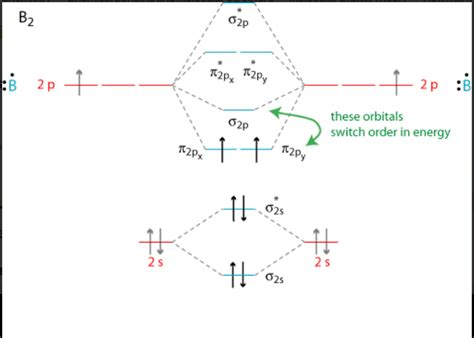
\includegraphics[width = 0.50 \textwidth]{sigma-pi-b2.jpg}
	\caption{Bonding orbitals (only for valence electrons) for $ \ch{B_2} $.}
	\label{bond-b2}
\end{figure}

Prendendo il caso di $ \ch{B_2} $ (o anche $ \ch{O_2} $), gli ultimi due elettroni di valenza vanno disposti per l'Aufbau su un orbitale $ \pi $ (o $ \pi^* $), il quale può però ospitare quattro elettroni: di conseguenza, per la prima regola di Hund essi occupano l'orbitale con spin paralleli. \\
Vengono osservati anche dimeri come $ \ch{Be_2} $ e $ \ch{Ne_2} $ che, nonostante un ordine di legame nullo, manifestano un debole legame non chimico (legame di van der Waals).

\paragraph{Potenziali analitici}

È possibile formulare alcuni modelli analitici per approssimare il potenziale adiabatico. Un esempio è il \textit{potenziale di Lennard-Jones}:
\begin{equation}
	V_\text{LJ}(R) = 4 \varepsilon \left[ \left( \frac{\sigma}{R} \right)^{12} - \left( \frac{\sigma}{R} \right)^6 \right]
\end{equation}
con $ \varepsilon \sim 1-100 \,\text{meV} $ e $ \sigma \sim 1-3 \ang $. Questo potenziale descrive i dimeri di atomi i cui orbitali sono completamente pieni (ovvero i gas nobili): essi infatti non formano legami covalenti, ma legami dovuti a deboli fluttuazioni indotte sui dipoli elettrici\footnotemark (che altrimenti sarebbero nulli). Ponendo $ V_\text{LJ}' = 0 $ si trova la distanza d'equilibrio $ R_\text{m} = \sqrt[6]{2} \sigma $ e la profondità della buca di potenziale $ V_\text{LJ}(R_\text{m}) = -\varepsilon $ (si noti che questi valori valgono per soli dimeri, in quanto molecole poliatomiche hanno geometrie più complesse). \\
Per descrivere legami covalenti si utilizza invece il \textit{potenziale di Morse}:
\begin{equation}
	V_\text{M}(R) = \mathcal{E}_d \left[ 1 - e^{-\beta (R - R_\text{m})} \right]^2
\end{equation}
dove $ \mathcal{E}_d $ è l'energia di dissociazione della molecola e $ \beta $ è un parametro legato alla frequenza caratteristica delle oscillazioni attorno al minimo di potenziale da $ \kappa = 2 \mathcal{E}_d \beta^2 $. A differenza di $ V_\text{LJ}(R) $, il potenziale di Morse ha un valore finito per $ R = 0 $.

\footnotetext{Un dipolo istantaneo $ \bs{\mu}_1 $ in un atomo induce un dipolo istantaneo indotto $ \bs{\mu}_2 $ sull'atomo adiacente: questo dipolo indotto avrà sempre verso opposto al primo dipolo, risultando dunque in un'interazione attrattiva tra di essi che scala come $ R^{-6} $.}

\subsubsection{Molecole diatomiche eteronucleari}

Sebbene i dimeri godano di una particolare simmetria per riflessioni, esistono anche molecole diatomiche eteronucleari. In questi casi, c'è un'asimmetria nella distribuzione di carica, poiché gli elettroni saranno maggiormente attratti da uno dei due atomi: come si vede in Fig. \ref{etero}, gli orbitali leganti si trovano energeticamente più vicini agli orbitali dell'atomo che li ha energeticamente più bassi, fino a casi limite come $ \ch{HF} $ in cui gli orbitali coincidono energeticamente. Si distingue quindi tra legami covalenti polari e legami ionici: di quest'ultimi si può dare una descrizione approssimata come di un completo trasferimento di carica dall'atomo meno elettronegativo a quello più elettronegativo (come in $ \ch{HF} $).

\begin{figure}
	\centering
	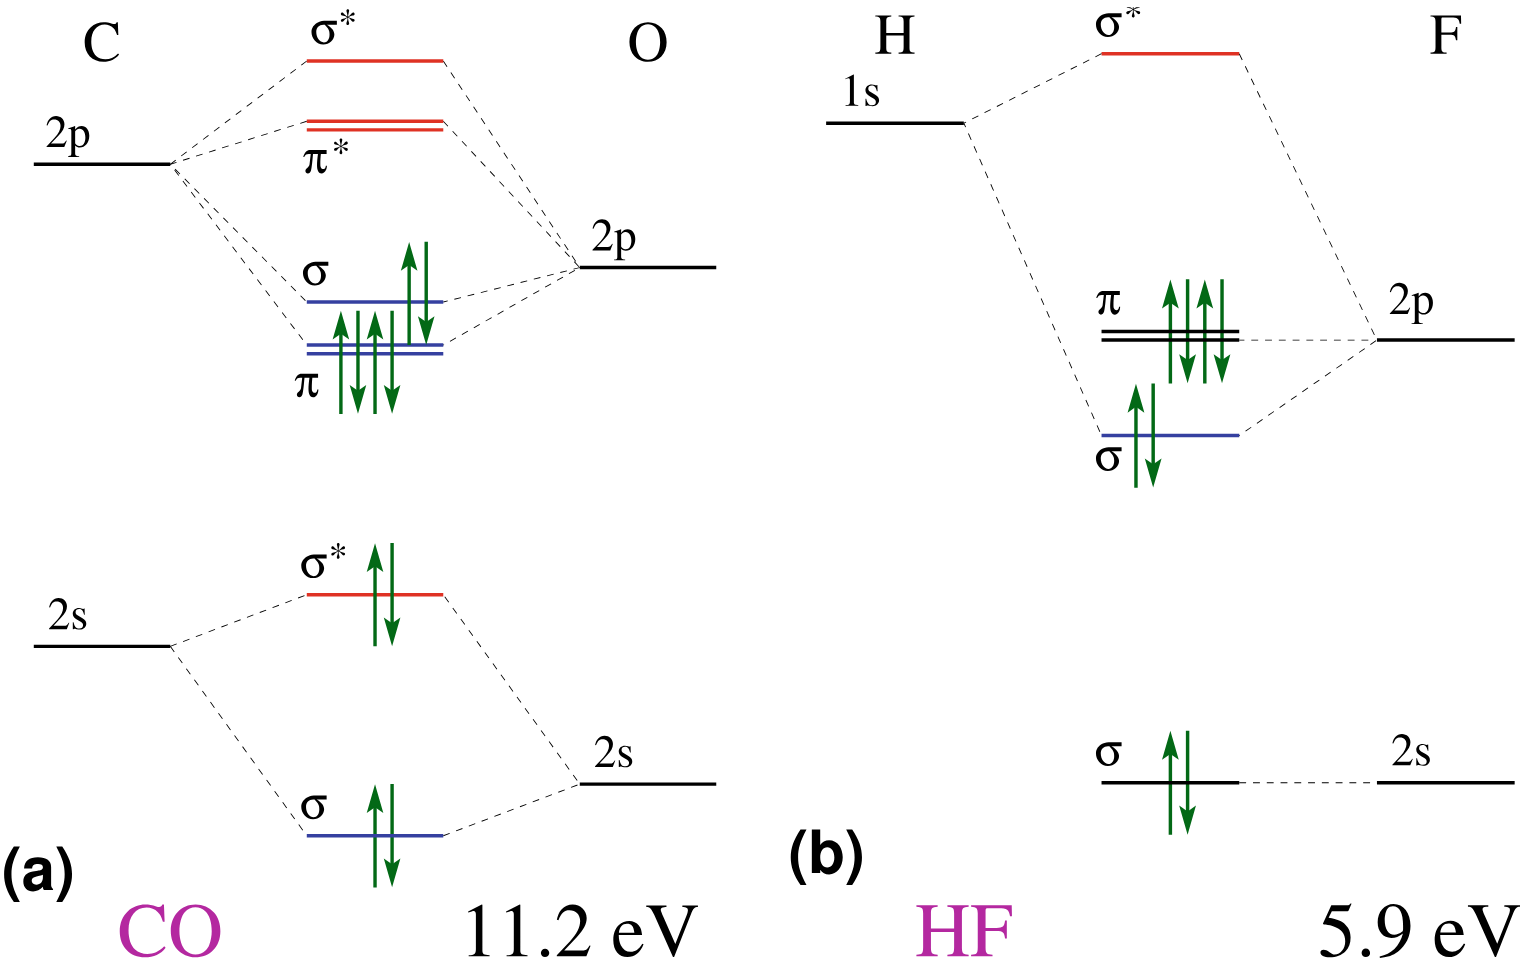
\includegraphics[width = 0.50 \textwidth]{eteronuclear.png}
	\caption{Bonding orbitals for eteronuclear diatomic molecules.}
	\label{etero}
\end{figure}

\subsection{Classificazione}

Nonostante la generale tendenza degli atomi ad attrarsi a grandi distanze e respingersi a corte distanze (Fig. \ref{ad-pot}), ci sono grosse differenze di distanze di equilibrio e profondità della buca di potenziale per i vari meccanismi di legame. \\
Se uno (o entrambi) dei due atomi è un gas nobile, allora il legame è di tipo dipolo-dipolo indotto (van der Waals), con una distanze d'equilibrio $ R_\text{m} \sim 250-400 \,\text{pm} $ grande ed energia di legame nell'ordine dei $ \text{meV} $. I gas nobili mantengono la forma di gas monoatomico fino a temperature relativamente basse, per poi formare dimeri in grado di condensarsi e solidificarsi. \\
Al contrario, alcuni atomi con shell non complete ($ \ch{N} $, $ \ch{O} $, $ \ch{F} $) tendono a formare molecole diatomiche con legami covalenti corti e molto forti (binding energy $ \sim \text{eV} $), molecole mantenute anche nelle fasi liquide e solide a basse temperature. Per la maggior parte degli altri atomi, l'energia extra guadagnata formando legami chimici multipli rende energeticamente conveniente formare legami metallici estesi (o anche solidi covalenti), piuttosto che molecole diatomiche.\\
Nel caso di molecole eteronucleari fortemente polari si può arrivare alla formazione di legami ionici, con un transferimento (totale o parziale) di carica da un'atomo all'altro: al pari dei legami covalenti e metallici, le distanze d'equilibrio sono $ R_\text{m} \sim 80-250 \,\text{pm} $ e le binding energies $ \sim 1-10\ev $.

\section{Spettri molecolari}

Si passa ora allo studio del moto dei due nuclei di una molecola diatomica, governato dall'Eq. \ref{eq:mol-nucl-eq}. Si noti che il potenziale adiabatico è indipendente dalla posizione del centro di massa della molecola (invarianza per traslazioni) e dall'orientazione nello spazio dell'asse molecolare (invarianza per rotazioni): di conseguenza, si può separare il moto in moto del centro di massa, che risulta in uno spettro continuo (il moto termico randomico del centro di massa genera l'allargamento delle linee spettrali per effetto Doppler), e moto relativo, il quale gode di simmetria sferica rispetto a $ \ve{R}_{12} $. Per quanto riguarda quest'ultimo, tramite la separazione delle variabili si può separare l'equazione nucleare in tre equazioni, di cui due angolari standard ed una radiale con potenziale adiabatico. Le soluzioni delle equazioni angolari sono le armoniche sferiche $ Y_{\ell,m_\ell} $, dove $ \ell $ è il momento angolare molecolare ed $ m_\ell \in [-\ell,\ell] $ la sua proiezione lungo l'asse molecolare. Per quanto riguarda l'equazione radiale, invece, data dall'Eq. \ref{eq:1-e-rad-eq} con $ V(r) \equiv V_\text{ad}(r) $ (ed $ r \equiv R_{12} $), si può considerare che il potenziale adiabatico presenta un minimo in un punto d'equilibrio finito $ R_{12} = R_\text{m} > 0 $, dunque si può considerare che la molecola studiata si trovi in un intorno di $ R_\text{m} $, così da poter ignorare variazioni del termine centrifugo $ \frac{\hbar^2 \ell (\ell + 1)}{2\mu R_{12}^2} $ ($ R_{12}^{-2} $ varia poco in un intorno di $ R_\text{m} > 0 $) ed approssimare il moto radiale come indipendente da $ \ell $; espandendo il potenziale attorno ad $ R_\text{m} $:
\begin{equation*}
	V_\text{ad}(R_{12}) = V_\text{ad}(R_\text{m}) + \frac{1}{2} \frac{d^2 V_\text{ad}(R)}{dR^2}\bigg\vert_{R = R_\text{m}} (R_{12} - R_\text{m})^2 + \dots \equiv V_\text{ad}(R_\text{m}) + \frac{1}{2} \kappa (R_{12} - R_\text{m})^2 + \dots
\end{equation*}
Si può dunque approssimare il potenziale con un potenziale armonico ed il sistema con un oscillatore armonico; definendo il numero quantico $ v \in \N_0 $ come il numero di nodi della funzione d'onda radiale, si trova lo spettro radiale vibrazionale:
\begin{equation}
	E_\text{vib}(v) = \hbar \omega \left( v + \frac{1}{2} \right)
\end{equation}
con $ \omega \equiv \sqrt{\kappa / \mu} $. Grandezze tipiche sono $ \hbar \omega \sim 20-400 \,\text{meV} $. Il termine centrifugo, invece, determina uno spettro rotazionale:
\begin{equation}
	E_\text{rot}(\ell) = \frac{\hbar^2 \ell (\ell + 1)}{2\mu R_\text{m}^2} \equiv \frac{\ve{L}^2}{2I}
\end{equation}
Questa è la cosiddetta approssimazione del rotatore rigido, in cui si definisce il momento d'inerzia $ I $: ciò è possibile poiché si è assunto che $ R_{12} \approx R_\text{m} $ privo di variazioni in un intorno di $ R_\text{m} $. Grandezze tipiche sono nell'ordine dei $ \text{meV} $: l'energia rotazionale più alta è quella del $ \ch{H_2} $, pari a $ 7 \,\text{meV} $.

\subsection{Spettro rotazionale e roto-vibrazionale}

Se si considerano transizioni adiabatiche, ovverosia transizioni in cui gli elettroni rimangono nel loro ground state, le molecole soddisfano le solite selection rules di dipolo elettrico: $ \Delta \ell = \pm 1 $.
Nel caso delle molecole diatomiche, l'operatore di dipolo elettrico è determinato dalla separazione tra i due nuclei e dalla loro differenza di carica: nel caso di molecole omonucleari tale differenza è nulla, dunque per esse non si osservano transizioni di dipolo elettrico\footnote{Questo è il motivo per cui l'aria (composta principalmente da $ \ch{N_2} $ e $ \ch{O_2} $) è altamente trasparente ai raggi IR; la trasparenza nel visibile e nel vicino UV è invece associata al grosso gap (vari $ \text{eV} $) che separa il ground state elettronico ed il primo stato eccitato elettronico.}. Inoltre, l'operatore di dipolo elettrico dipende dalla distanza $ R_{12} $: in un intorno di $ R_\text{m} $, si può espandere come:
\begin{equation*}
	\ve{d}(R_{12}) = \ve{d}(R_\text{m}) + \frac{\dd \ve{d}(R)}{\dd R}\bigg\vert_{R = R_\text{m}} (R_{12} - R_\text{m}) + \dots
\end{equation*}
In questo modo, come prima si erano eliminate le anarmonicità meccaniche, ora si sono eliminate le anarmonicità elettriche. Il termine costante $ \ve{d}(R_\text{m}) $ dà luogo allo spettro rotazionale puro (poiché $ \braket{\text{f} | \ve{d}(R_\text{m}) | \text{f}} \neq 0 $ solo se $ v_\text{f} = v_\text{i} $), mentre il termine proporzionale a $ R_{12} - R_\text{m} $ determina lo spettro roto-vibrazionale\footnote{Più precisamente, il termine $ \sim (R_{12} - R_\text{m})^n $ ha elemento di matrice non-nullo solo se $ v_\text{f} - v_\text{i} = \pm n $.}. \\
Gli spettri rotazionali e vibrazionali delle molecole si osservano principalmente come spettri d'assorbimento, dato che il basso rate di emissione spontanea (decay rate $ \sim \mathcal{E}_\text{if}^3 $) determina una preponderanza di fenomeni di decadimento radiation-less (es.: collisioni tra molecole).

\subsubsection{Spettro rotazionale}

Gli spettri puramente rotazionali si osservano nella regione del lontano IR e sono associati a transizioni con $ \Delta v = 0 $ e $ \Delta \ell = \pm 1 $. La differenza energetica tra $ \ket{\ell_\text{i}} \equiv \ket{\ell} $ e $ \ket{\ell_\text{f}} \equiv \ket{\ell + 1} $ è:
\begin{equation}
	\Delta E_\text{rot}(\ell) = \frac{\hbar^2}{I} (\ell + 1)
\end{equation}
Di conseguenza, lo spettro rotazionale di un campione di molecole in vari stati rotazionali iniziali sarà composto da una serie di righe d'assorbimento equispaziate, con una separazione energetica $ \hbar^2 / I $ che è il doppio della tipica scala energetica rotazionale $ \hbar^2 / 2I $. Una misura di tale separazione permette di stimare $ I $ e, di conseguenza, la distanza interatomica d'equilibrio $ R_\text{m} $. \\
L'equispaziatura dei salti energetici rotazionali permette di definire una \textit{temperatura rotazionale}, determinata da tale scala energetica:
\begin{equation}
	\theta_\text{rot} \defeq \frac{\hbar^2}{I k_\text{B}}
\end{equation}
dove $ k_\text{B} = 8.617 \cdot 10^{-5} \ev/\text{K} $ è la costante di Boltzmann. La scala di temperatura tipica è $ \sim 12 \,\text{K} $ (per energie $ \sim 1 \,\text{meV} $). Questa temperatura va confrontata con quella a cui si svolge l'esperimento: se $ T \ll \theta_\text{rot} $ il sistema si troverà sostanzialmente nel suo ground state, mentre se $ T \gg \theta_\text{rot} $ saranno popolati con buona probabilità molti livelli eccitati.

\begin{figure}
	\centering
	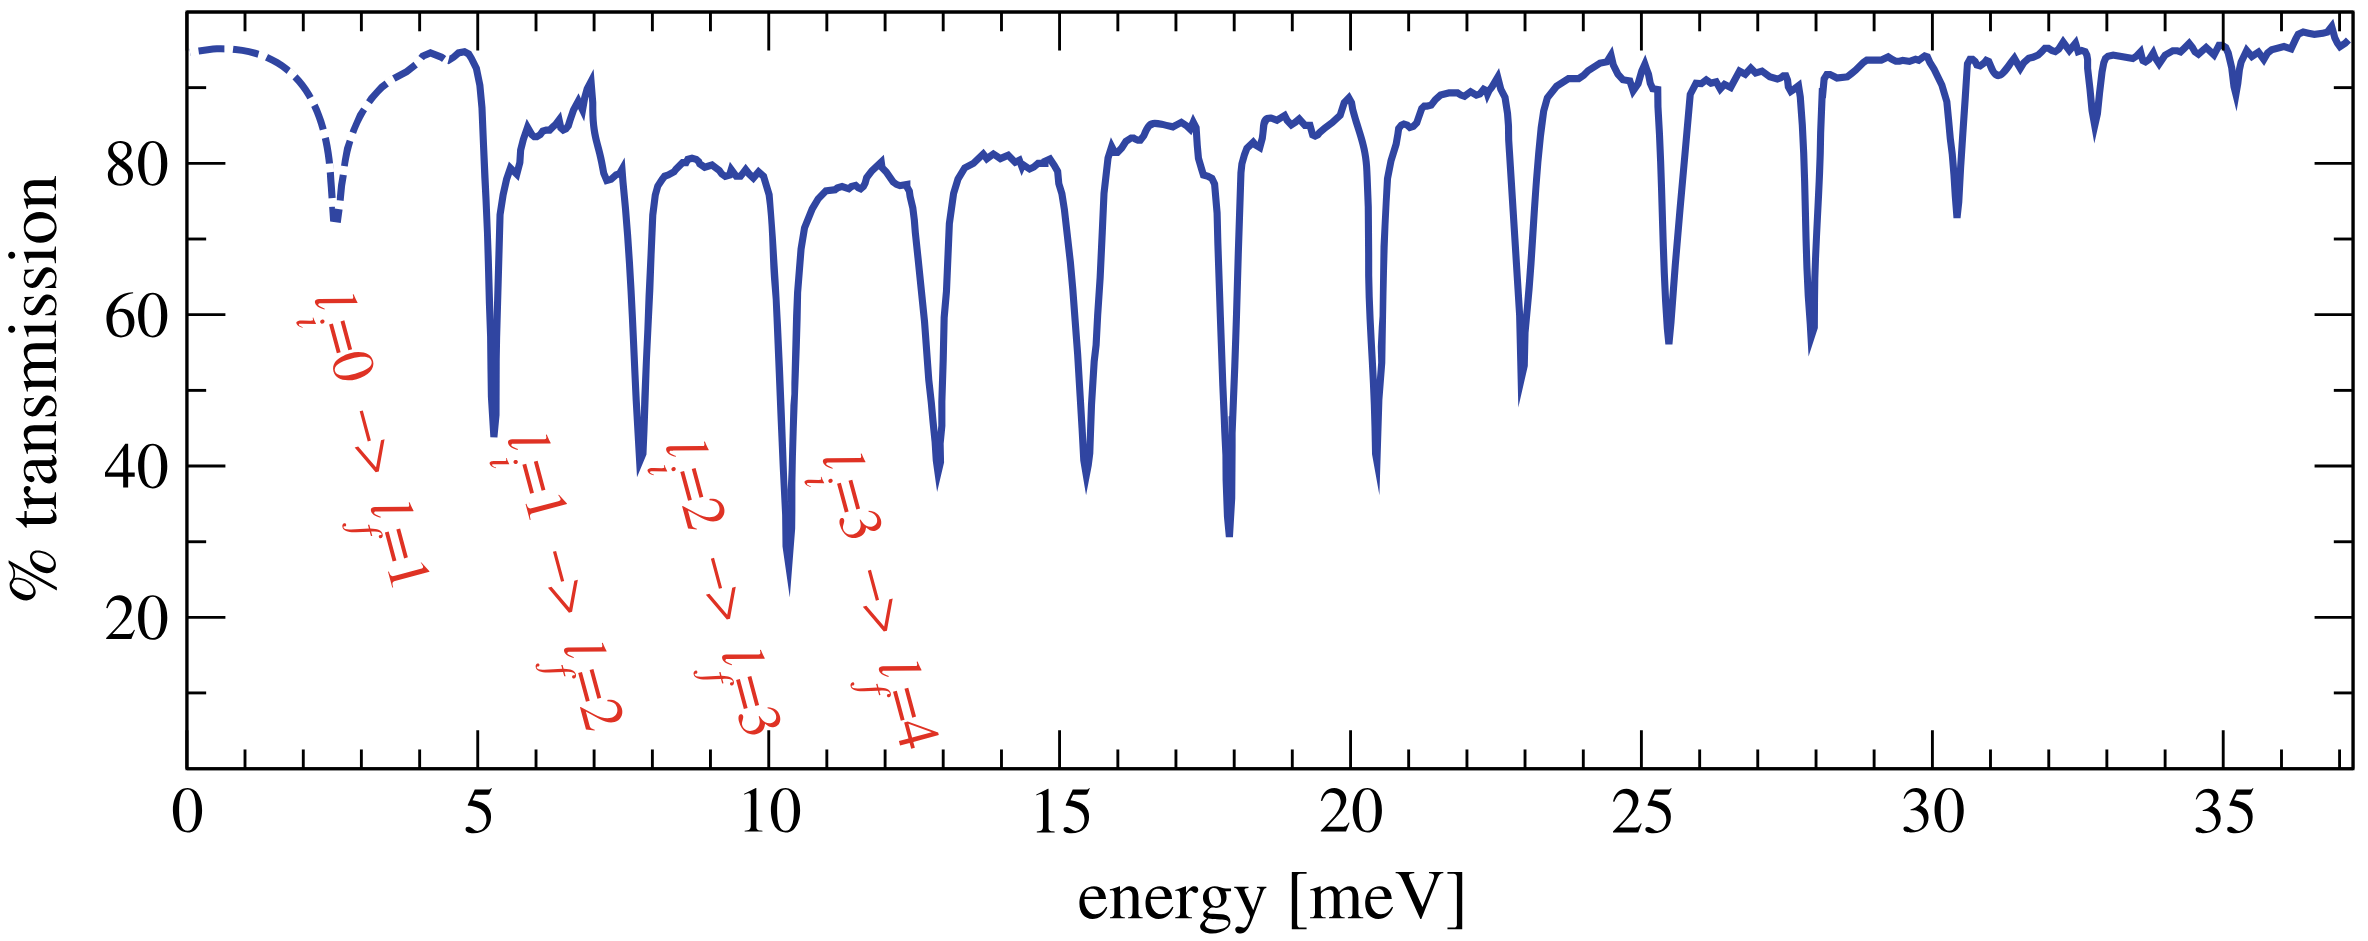
\includegraphics[width = 0.80 \textwidth]{rot-spectr.png}
	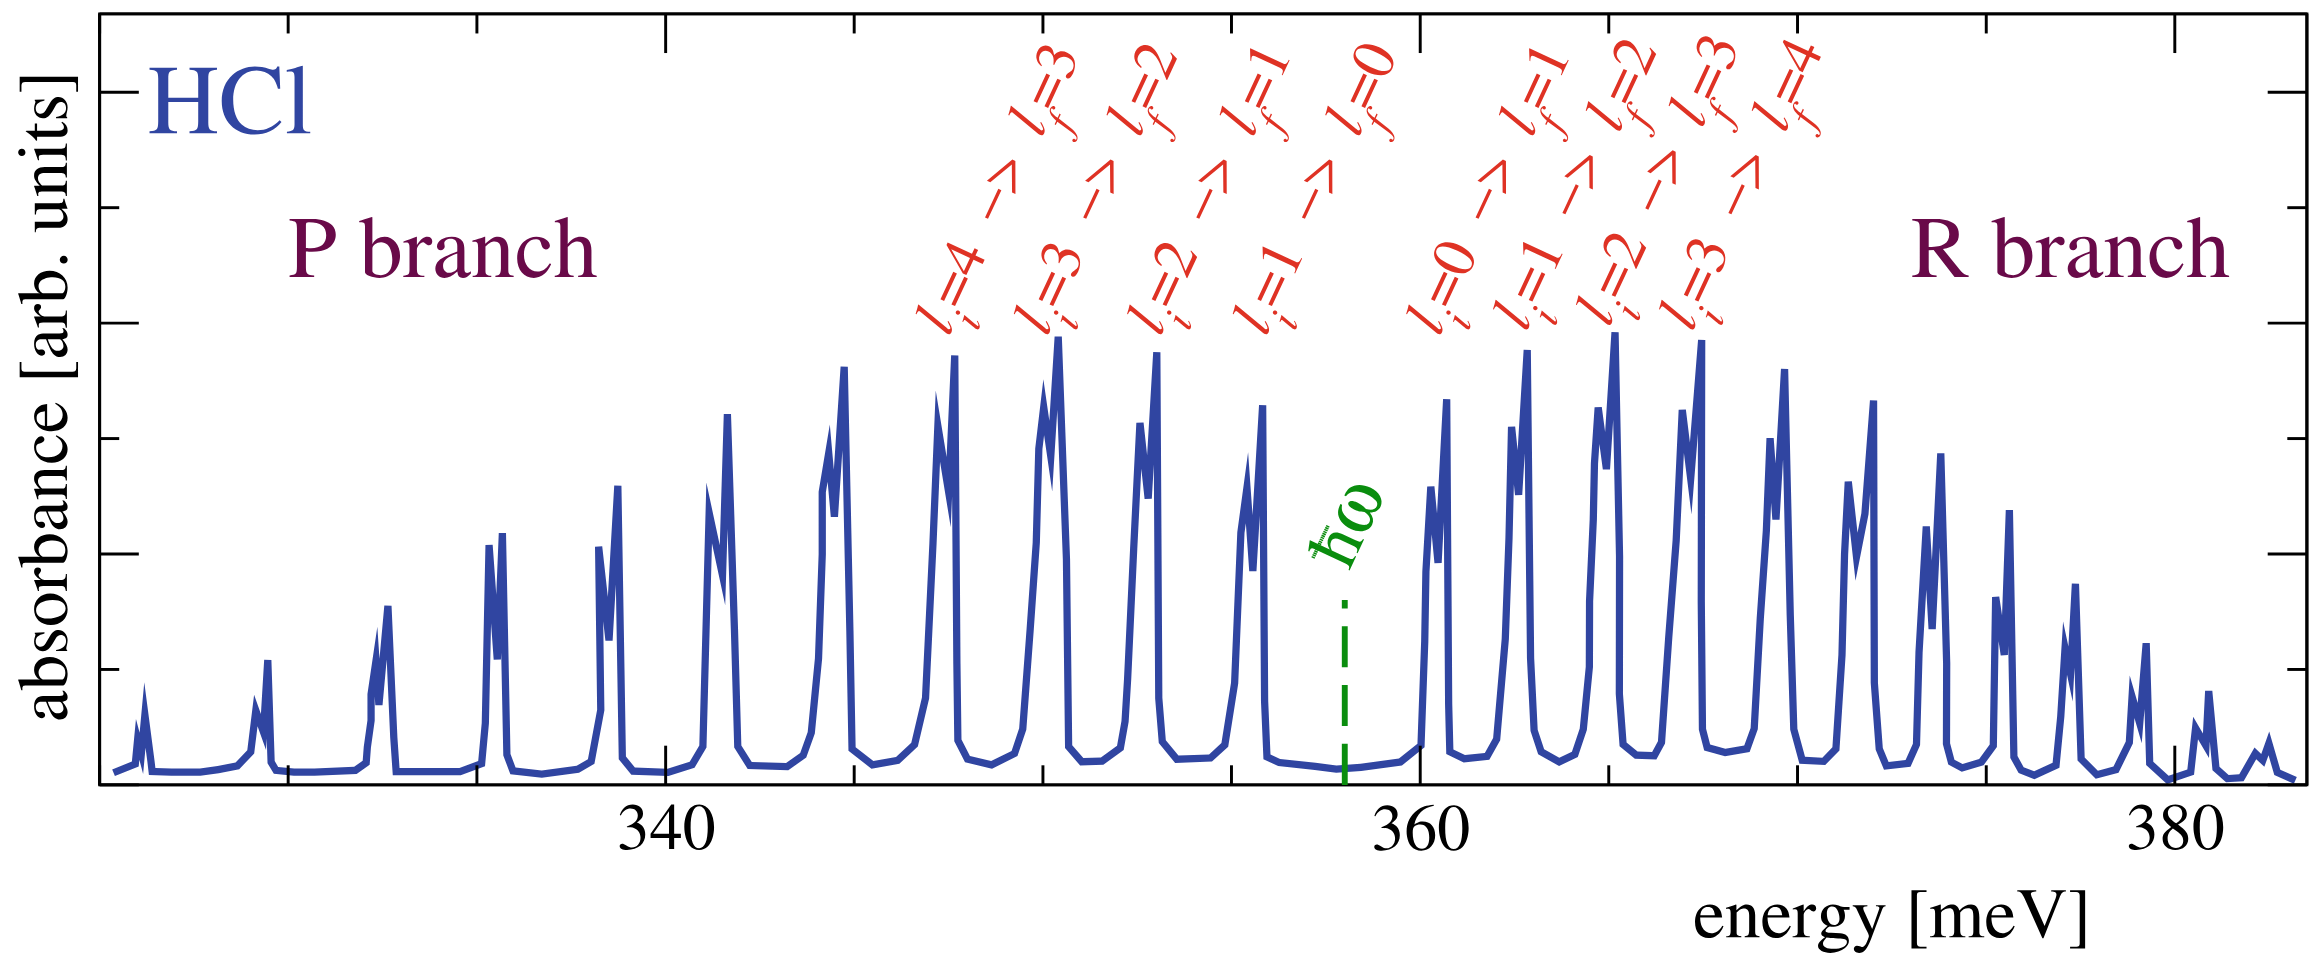
\includegraphics[width = 0.80 \textwidth]{rot-vib-spectr.png}
	\caption{Observed purely-rotational (above) and roto-vibrational (below) absorption spectrum of gas-phase $ \ch{HCl} $.}
	\label{rot-vib-sp}
\end{figure}
\begin{figure}
	\centering
	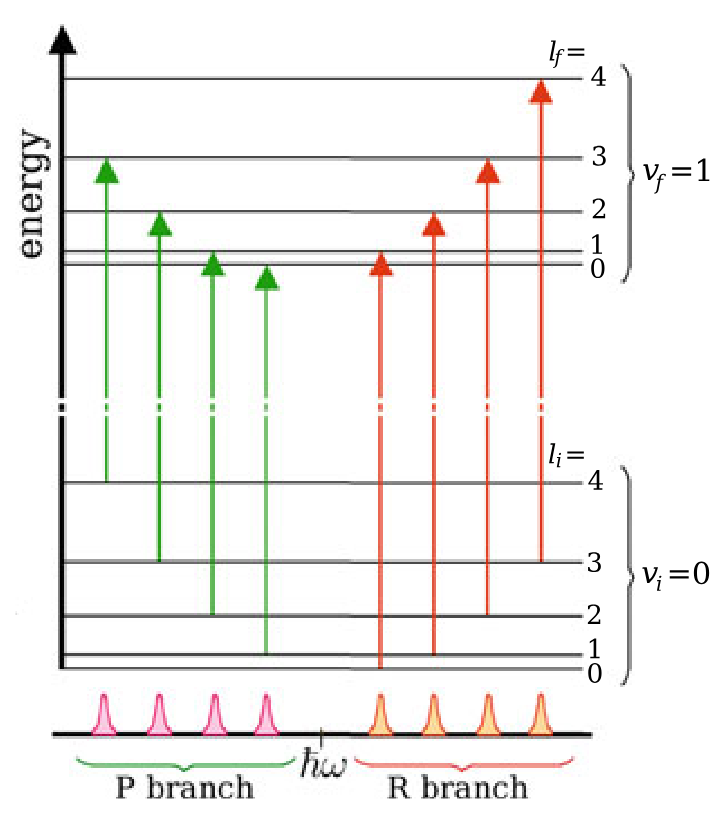
\includegraphics[width = 0.40 \textwidth]{rot-vib-spectr-det.png}
	\caption{Scheme of electric-dipole transitions between rotational levels $ \ket{v = 0} \rightarrow \ket{v = 1} $.}
	\label{rot-vib-det}
\end{figure}

\subsubsection{Spettro roto-vibrazionale}

Gli spettri roto-vibrazionali si osservano nella regione del vicino IR e sono associati a transizioni $ \Delta v > 0 $ e $ \Delta \ell = \pm 1 $: la maggior parte dell'intensità è data dalle transizioni $ \Delta v = 1 $, mentre le overtone transitions $ \Delta v > 1 $ sono più deboli. \\
Come si vede in Figg. \ref{rot-vib-sp}-\ref{rot-vib-det}, una volta fissata una transizione con $ \Delta v = 1 $, essa è $ \virgolette{decorata} $ da varie transizioni $ \Delta \ell = \pm 1 $, essendo il campione composto di molecole in vari stati rotazionali iniziali: le transizioni con $ \Delta \ell = -1 $ formalo la P-branch, mentre quelle con $ \Delta \ell = +1 $ la R-branch. Si noti l'assenza di una transizione piccata in $ \hbar \omega $, la quale sarebbe associata ad una transizione dipolo-proibita $ \Delta \ell = 0 $. \\
In presenza di uno spettrometro a bassa risoluzione, non si riescono a distinguere le singole righe rotazionali e si osserva un'unica riga vibrazionale. \\
Analogamente allo spettro rotazionale, si può definire una \textit{temperatura vibrazionale}:
\begin{equation}
	\theta_\text{vib} \defeq \frac{\hbar \omega}{k_\text{B}}
\end{equation}
In questo caso le energie si attestano su $ \sim 0.5\ev $, dunque $ \theta_\text{vib} \sim 6000 \,\text{K} $.

\subsubsection{Molecole poliatomiche}

Nel caso di molecole poliatomiche, in generale il potenziale adiabatico dipenderà sia dalle distanze relative tra i vari nuclei che dagli angoli tra tali distanze, rendendo la trattazione del problema molto più complessa. In particolare, ci saranno vari modi normali d'oscillazione attorno al minimo multidimensionale di $ V_\text{ad} $, ciascuno modellabile da un oscillatore armonico indipendente.

\subsection{Eccitazioni elettroniche}

Fotoni nel range del visibile e UV possono provocare eccitazioni dello stato elettronico delle molecole: queste eccitazioni possono essere modellate dalla promozione di un elettrone da un orbitale molecolare occupato ad uno vuoto. Una transizione $ \psi_e^{(a)} \rightarrow \psi_e^{(b)} $ provoca un cambiamento di superficie potenziale adiabatica: data la time-scale estremamente piccola, i nuclei non hanno tempo di muoversi, dunque (come in Fig. \ref{elec-ex}) tale cambiamento è $ \virgolette{verticale} $ in $ R_{12} $. Dato che in generale $ R_\text{m}^{(a)} \neq R_\text{m}^{(b)} $, solitamente le transizioni elettroniche sono accompagnate da transizioni vibrazionali dovute alla variazione della geometria d'equilibrio.

\begin{figure}
	\centering
	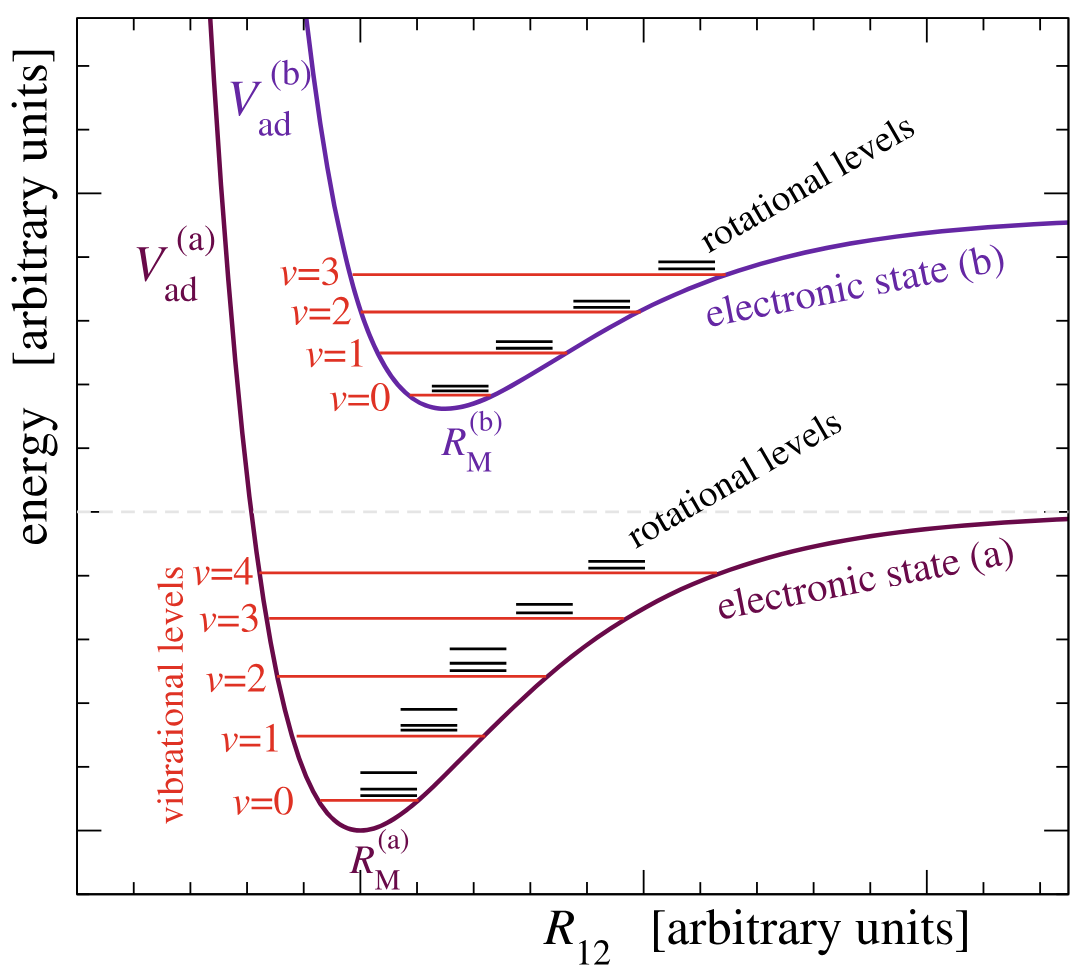
\includegraphics[width = 0.50 \textwidth]{electr-exc.png}
	\caption{Adiabatic potential surfaces for $ \psi_e^{(a)} \rightarrow \psi_e^{(b)} $.}
	\label{elec-ex}
\end{figure}
\begin{figure}
	\centering
	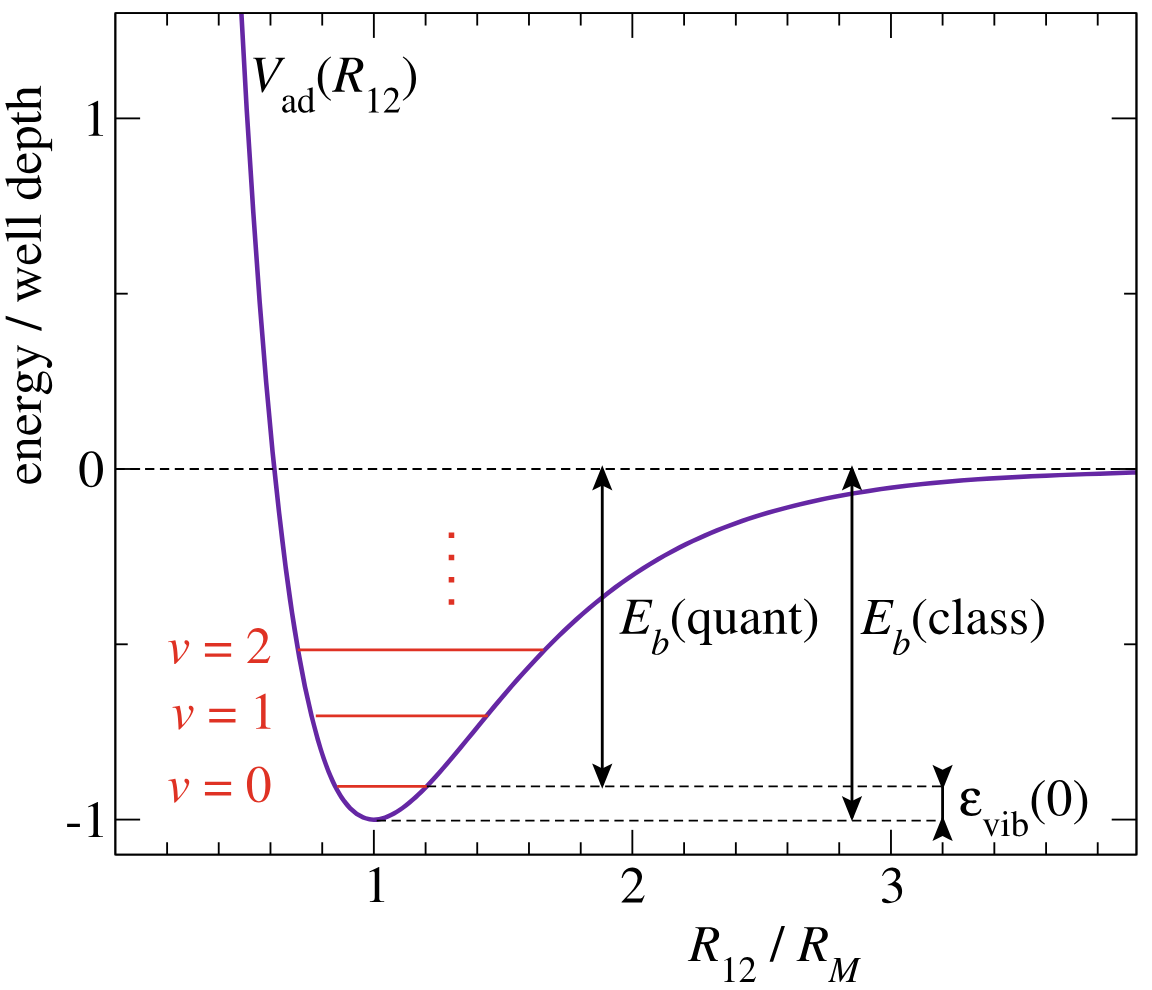
\includegraphics[width = 0.50 \textwidth]{zero-point-eff.png}
	\caption{Quantum zero-point vibrational energy.}
	\label{zero-p}
\end{figure}

\subsubsection{Effetti di punto-zero}

Come si vede in Fig. \ref{zero-p}, la binding energy $ E_b $ di una molecola diatomica è leggermente inferiore alla profondità $ V_\text{ad}(\infty) - V_\text{ad}(R_\text{m}) $ della buca di potenziale adiabatico. I due valori coinciderebbero se le masse dei nuclei fossero infinite (o se essi fossero oggetti classici), ma per il principio d'indeterminazione è presente un'energia vibrazionale di punto-zero $ E_\text{vib}(0) = \frac{\hbar \omega}{2} $, la quale spiega la piccola differenza tra i due valori. \\
Sperimentalmente, si possono indagare questi effetti di punto-zero andando a variare la massa degli isotopi coinvolti, dato che $ \omega \propto \mu^{-1/2} $ mentre $ V_\text{ad}(R_{12}) $ non dipende da esso. Uno degli effetti di punto-zero più grandi si ha nel $ \ch{^4He_2} $: la buca di potenziale adiabatico è profonda circa $ 900 \,\mu\text{eV} $, ma il sistema è estremamente debolmente legato con $ E_b \simeq 0.1 \,\mu\text{eV} $, dunque $ E_\text{vib}(0) $ bilancia quasi completamente l'attrazione adiabatica. A confermare la dipendenza da $ \mu $, per il più leggero $ \ch{^3He_2} $ non si osservano stati legati (l'energia di punto-zero è più grande della buca di potenziale adiabatico).













\part{Solidi}
\pagestyle{body}

\chapter{Fisica Statistica}
\selectlanguage{italian}

La Fisica Statistica (quantistica) fornisce le relazioni tra le proprietà medie microscopiche di un sistema con le sua dinamica macroscopica. In particolare, si fanno due assunzioni fondamentali (per rendere la trattazione indipendente dalle condizioni iniziali del sistema):
\begin{enumerate}
	\item equilibrio: il sistema ha superato tutti i transienti e tutte le quantità collettive (es.: pressione) hanno delle piccole fluttuazioni attorno ad un valore ben definito;
	\item ergodicità: le medie temporali delle osservabili coincidono con le medie d'ensemble.
\end{enumerate}

\section{Operatore densità}

Si consideri un sistema quantistico di $ N $ corpi (con $ N \sim N_\text{A} \simeq 6.022 \cdot 10^{23} $). Detti $ \{\ket{\psi_i}\}_{i \in \mathcal{I}} $ i possibili stati in cui si può trovare il sistema e detta $ w_i \in [0,1] $ la probabilità che il sistema si trovi in $ \ket{\psi_i} $ (condizione di normalizzazione $ \sum_{i \in \mathcal{I}} w_i = 1 $), l'\textit{expectation value} di un'osservabile $ \hat{B} $ sarà:
\begin{equation}
	[B] \defeq \sum_{i \in \mathcal{I}} w_i \braket{\psi_i | \hat{B} | \psi_i}
\end{equation}
Data un set completo ortonormale $ \{\ket{b_j}\}_{j \in \mathcal{J}} $ di autostati di $ \hat{B} $, allora $ \hat{B} = \sum_{j \in \mathcal{J}} b_j \ket{b_j}\bra{b_j} $, ovvero:
\begin{equation}
	[B] = \sum_{i \in \mathcal{I}} \sum_{j \in \mathcal{J}} w_i b_j \abs{\braket{b_j | \psi_i}}^2
	\label{eq:b-exp-val}
\end{equation}

\begin{definition}{Operatore densità}{}
	Si definisce l'\textit{operatore statistico} (o operatore densità) come:
	\begin{equation}
		\hat{\rho} \defeq \sum_{i \in \mathcal{I}} w_i \ket{\psi_i}\bra{\psi_i}
	\end{equation}
\end{definition}

\begin{theorem}{Expectation value}{}
	L'expectation value di un'osservabile $ \hat{B} $ può essere espresso come:
	\begin{equation}
		[B] = \tr(\hat{\rho} \hat{B})
	\end{equation}

	\tcblower

	\begin{proof}
		Dall'Eq. \ref{eq:b-exp-val} (e ricordando che $ \{\ket{b_j}\}_{j \in \mathcal{J}} $ è base ortonormale di $ \hilb $):
		\begin{equation*}
			[B] = \sum_{i \in \mathcal{I}} \sum_{j \in \mathcal{J}} w_i b_j \braket{b_j | \psi_i} \braket{\psi_i | b_j} = \sum_{j \in \mathcal{J}} b_j \braket{b_j | \hat{\rho} | b_j} = \sum_{j \in \mathcal{J}} \braket{b_j | \hat{\rho} \hat{B} | b_j} \eqdef \tr(\hat{\rho} \hat{B})
		\end{equation*}
	\end{proof}
\end{theorem}

Un corollario banale è che $ \tr{\hat{\rho}} = 1 $ (con $ \hat{B} \equiv \id_\hilb $). Inoltre, si vede che per un sistema in uno stato puro, ovvero $ w_i = \delta_{i,i_0} $ per un certo $ i_0 \in \mathcal{I} $, allora $ \hat{\rho} = \ket{\psi_{i_0}}\bra{\psi_{i_0}} $ è un proiettore (dunque idempotente: $ \hat{\rho}^2 = \hat{\rho} $).

\section{Ensemble all'equilibrio}

\subsection{Ensemble microcanonico}

Si consideri un sistema isolato ad energia fissata $ E $ con una piccola incertezza $ \Delta E $: questo viene detto \textit{ensemble microcanonico}. Dall'ipotesi di ergodicità deriva che tutti gli stati amessi dalla conservazione dell'energia sono equiprobabili:
\begin{equation}
	w_i =
	\begin{cases}
		\frac{1}{\Omega} & E_i \in [E - \Delta E/2 , E + \Delta E/2] \\
		0 & E_i \notin [E - \Delta E/2 , E + \Delta E/2]
	\end{cases}
	\label{eq:microcanon-ens}
\end{equation}
dove $ \Omega = \Omega(E, \Delta E) $ è il numero di stati accessibili nello spazio delle fasi posta la condizione energetica.

\subsection{Ensemble canonico}

Si consideri ora un sistema $ \text{S} $ al'interno dell'universo $ \text{U} $ e sia $ \text{W} \equiv \text{U} - \text{S} $. Assumendo che $ \mathcal{H}_\text{U} = \mathcal{H}_\text{S} + \mathcal{H}_\text{W} + \mathcal{H}_\text{SW} \approx \mathcal{H}_\text{S} + \mathcal{H}_\text{W} $, ovvero che sia $ \text{S} $ che $ \text{W} $ siano considerabili isolati, allora questi saranno descritti dalla distribuzione microcanonica Eq. \ref{eq:microcanon-ens}.

\begin{theorem}{Distribuzione canonica}{}
	Dato uno stato possibile $ \ket{\psi_m} $ con energia $ E_m $ del sistema $ \text{S} $, la sua probabilità è data dalla \textit{distribuzione di Boltzmann}:
	\begin{equation}
		P_m^\text{S} = \frac{1}{Z} e^{- \beta E_m}
	\end{equation}
	dove $ \beta = \beta(T) $ e $ Z $ è la \textit{funzione di partizione} del sistema $ \text{S} $:
	\begin{equation}
		Z \defeq \sum_{i \in \mathcal{I}} e^{- \beta E_i} \equiv \tr e^{- \beta \mathcal{H}}
		\label{eq:part-func-states}
	\end{equation}

	\tcblower

	\begin{proof}
		Dall'ipotesi di interazione debole tra $ \text{S} $ e $ \text{W} $ si ha $ P^\text{U}(E) = P^\text{S}(E_m) P^\text{W}(E - E_m) $, dunque, essendo questi sistemi microcanonici:
		\begin{equation*}
			P_m^\text{S} = \frac{P^\text{U}(E)}{P^\text{W}(E-E_m)} = \frac{\Omega_\text{W}(E-E_m,\Delta E)}{\Omega_\text{U}(E,\Delta E)}
		\end{equation*}
		Assumendo $ E_m \ll E $ si può sviluppare in serie:
		\begin{equation*}
			\ln \Omega_\text{W}(E - E_m , \Delta E) = \ln \Omega_\text{W}(E , \Delta E) - \beta E_m + o(E_m^2)
			\qquad \qquad
			\beta \equiv \frac{\pa}{\pa x}\bigg\vert_{x = E} \ln \Omega_\text{W}(x , \Delta E)
		\end{equation*}
		Esponenziando e sostituendo nell'equazione precedente si ottiene:
		\begin{equation*}
			P_m^\text{S} = \frac{\Omega_\text{W}(E , \Delta E)}{\Omega_\text{U}(E, \Delta E)} e^{- \beta E_m} \equiv \frac{1}{Z} e^{- \beta E_m}
		\end{equation*}
		Il fattore iniziale non dipende da $ \ket{m} $, dunque è un fattore puramente di normalizzazione. Dalla condizione di normalizzazione $ \sum_{i \in \mathcal{I}} P_i^\text{S} = 1 $ si trova la tesi.
	\end{proof}
\end{theorem}

Si noti che nell'Eq. \ref{eq:part-func-states} la sommatoria è su tutti gli stati, includendo in particolare quelli degeneri. Si può passare ad una sommatoria sulle energie ammesse definendo la degenerazione del livello energetico $ E $ come $ g(E) $, così che:
\begin{equation}
	Z = \sum_E g(E) e^{- \beta E}
\end{equation}
Inoltre, sebbene $ P_m^\text{S} $ dipenda da tutti i possibili valori di energia, il rapporto di probabilità $ P_m^\text{S} / P_n^\text{S} = e^{-\beta (E_m - E_n)} $ dipende solo da $ \Delta E_{mn} \equiv E_m - E_n $. \\
L'operatore densità dell'ensemble canonico (di Gibbs) è diagonale nell'autobase di $ \mathcal{H} $:
\begin{equation}
	\hat{\rho}_\text{Gibbs} = \sum_{m \in \mathcal{I}} \frac{e^{-\beta E_m}}{Z} \ket{m}\bra{m} \equiv \frac{e^{-\beta \mathcal{H}}}{\tr e^{-\beta \mathcal{H}}}
	\label{eq:op-dens-gibbs}
\end{equation}

\begin{example}{Sottosistemi isolati}{}
	Si consideri $ \text{S} = \text{S}_1 \cup \text{S}_2 $, con $ \text{S}_1 $ ed $ \text{S}_2 $ isolati. Allora:
	\begin{equation*}
		P_{(m_1,m_2)}^\text{S} = P_{m_1}^{\text{S}_1} P_{m_2}^{\text{S}_2} = \frac{1}{Z_1 Z_2} e^{-\beta (E_{m_1} + E_{m_2})}
	\end{equation*}
	confermando che $ E_{(m_1,m_2)} = E_{m_1} + E_{m_2} $ ($ \beta_1 = \beta_2 = \beta $ all'equilibrio). Dunque la distribuzione di Boltzmann riproduce i risultati intuitivi. Si noti inoltre che la funzione di partizione è una funzione moltiplicativa ($ Z_{1,2} = Z_1 Z_2 $), così che il suo logaritmo sia additivo ($ \ln Z_{1,2} = \ln Z_1 + \ln Z_2 $).
\end{example}

\subsection{Termodinamica}

È possibile ricavare le principali quantità termodinamiche a partire dalla funzione di partizione e dall'operatore densità.

\begin{proposition}{Energia interna}{}
	L'energia interna media è:
	\begin{equation}
		U = - \frac{\pa}{\pa \beta} \ln Z
		\label{eq:int-en-z}
	\end{equation}

	\tcblower

	\begin{proof}
		Definendo $ U \equiv [\mathcal{H}] $:
		\begin{equation*}
			U = \tr(\hat{\rho}_\text{Gibbs} \mathcal{H}) = \sum_{m \in \mathcal{I}} P_m E_m = \frac{\sum_{m \in \mathcal{I}} E_m e^{-\beta E_m}}{\sum_{m \in \mathcal{I}} e^{- \beta E_m}} = - \frac{1}{Z} \frac{\pa Z}{\pa \beta} = - \frac{\pa}{\pa \beta} \ln Z
		\end{equation*}
	\end{proof}
\end{proposition}

Essendo $ \ln Z $ additivo su sistemi isolati, l'energia interna è correttamente una quantità termodinamica estensiva. Si vede inoltre che l'energia interna è una funzione non crescente di $ \beta $:
\begin{equation*}
	\frac{\pa U}{\pa \beta} = - \frac{\pa^2}{\pa \beta^2} Z = \frac{1}{Z^2} \left[ -Z \sum_{m \in \mathcal{I}} E_m^2 e^{-\beta E_m} + \left( \sum_{m \in \mathcal{I}} E_m e^{-\beta E_m} \right)^2 \right] = - [\mathcal{H}^2] + [\mathcal{H}]^2 = - [(\mathcal{H} - [\mathcal{H}])^2] \le 0
\end{equation*}

\begin{lemma}[before upper = {\tcbtitle}]{}{}
	\begin{equation}
		\beta = \frac{1}{k_\text{B} T}
	\end{equation}

	\tcblower

	\begin{proof}
		Si definisca l'energia libera $ F \equiv - \frac{1}{\beta} \ln Z $, così che $ U = \frac{\pa}{\pa \beta} (\beta F) $. D'altro canto, dalla Termodinamica si ha $ U - TS = F $, con $ S = - \frac{\pa F}{\pa T} $ l'entropia, dunque:
		\begin{equation*}
			\frac{F}{T} = \frac{U}{T} - S
			\quad \Rightarrow \quad
			U = \frac{\pa}{\pa(1/T)} \frac{F}{T} = \frac{\pa}{\pa \beta} (\beta F)
			\quad \Rightarrow \quad
			\beta \propto \frac{1}{T}
		\end{equation*}
		Nel limite classico si trova la corretta costante di proporzionalità.
	\end{proof}
\end{lemma}

\begin{proposition}{Calore specifico}{}
	Il calore specifico (a volume costante) è:
	\begin{equation}
		c_V = k_\text{B} \beta^2 \frac{\pa^2}{\pa \beta^2} \ln Z
		\label{eq:cal-spec-z}
	\end{equation}

	\tcblower

	\begin{proof}
		Ricordando che $ c_V \defeq \frac{\pa U}{\pa T} $ basta notare che $ \frac{\pa}{\pa T} = \frac{\pa \beta}{\pa T} \frac{\pa}{\pa \beta} = - \frac{1}{k_\text{B} T^2} \frac{\pa}{\pa \beta^2} $, ovvero:
		\begin{equation}
			\frac{\pa}{\pa T} = - k_\text{B} \beta^2 \frac{\pa}{\pa \beta}
		\end{equation}
	\end{proof}
\end{proposition}

È anche possibile dare una definizione più generale di entropia. Innanzitutto, dato che $ F = U - TS $, per l'ensemble canonico si trova:
\begin{equation}
	S = \frac{U}{T} + k_\text{B} \ln Z
	\label{eq:entropy-canon-ens}
\end{equation}
Questa può però essere generalizzata anche per sistemi non all'equilibrio.

\begin{definition}{Entropia}{}
	Dato un sistema con operatore densità $ \hat{\rho} $, si definisce l'\textit{entropia} come:
	\begin{equation}
		S \defeq - k_\text{B} \tr(\hat{\rho} \ln \hat{\rho})
	\end{equation}
\end{definition}

Sulla base degli autostati di $ \hat{\rho} $ (autostati $ \ket{\rho_m} $ con autovalori $ P_m $), l'entropia è:
\begin{equation}
	S = - k_\text{B} \sum_{m \in \mathcal{I}} P_m \ln P_m
\end{equation}

\begin{example}{Stato puro}{}
	Per uno stato puro $ P_m = \delta_{m,m_0} $, dunque correttamente $ S = -k_\text{B} \ln 1 = 0 $.
\end{example}

\begin{example}{Ensemble microcanonico}{}
	Per un ensemble microcanonico $ P_m = \frac{1}{\Omega} \,\,\forall m \in \mathcal{I} \,:\, \abs{\mathcal{I}} = \Omega $, dunque:
	\begin{equation*}
		S = - k_\text{B} \sum_{m = 1}^\Omega \frac{1}{\Omega} \ln \frac{1}{\Omega} = k_\text{B} \Omega \frac{1}{\Omega} \ln \Omega = k_\text{B} \ln \Omega
	\end{equation*}
	che è proprio l'equazione di Boltzmann.
\end{example}

\begin{example}{Ensemble canonico}{}
	Per l'ensemble canonico l'operatore densità è quello di Gibbs (Eq. \ref{eq:op-dens-gibbs}):
	\begin{equation*}
		S = - k_\text{B} \sum_{m \in \mathcal{I}} \frac{e^{-\beta E_m}}{Z} \ln \frac{e^{-\beta E_m}}{Z} = \frac{k_\text{B}}{Z} \sum_{m \in \mathcal{I}} e^{-\beta E_m} (\beta E_m + \ln Z) = k_\text{B} \beta [\mathcal{H}] + k_\text{B} \frac{Z \ln Z}{Z} = \frac{U}{T} + k_\text{B} \ln Z
	\end{equation*}
	che coincide con l'Eq. \ref{eq:entropy-canon-ens}. Si può dimostrare che $ \hat{\rho}_\text{Gibbs} $ è l'operatore densità che massimizza l'entropia per una data $ U = \tr(\hat{\rho}\mathcal{H}) $ fissata (oltre a $ N $ e $ V $): questo conferma il secondo principio della termodinamica, poiché un sistema generico descritto da $ \hat{\rho} $ tenderà all'ensemble canonico, ovverosia all'equilibrio, massimizzando l'entropia.
\end{example}

\section{Sistemi ideali}

Un sistema di $ N $ particelle si dice \textit{ideale} se si può separare:
\begin{equation}
	\mathcal{H} = \sum_{i = 1}^N \mathcal{H}_i \,:\, [\mathcal{H}_i , \mathcal{H}_j] = 0
\end{equation}
dove $ \mathcal{H}_i $ descrive soltanto i gradi di libertà della particella $ i $-esima. Lo spettro di questa Hamiltoniana è $ E_{\alpha_1, \dots, \alpha_N} = E_{\alpha_1} + \dots + E_{\alpha_N} $, ed inoltre si definisce il numero di occupazione $ n_k $ del livello energetico $ E_k $, $ k \in \mathcal{I} \subset \N $, così da poter scrivere la funzione di partizione del sistema come:
\begin{equation}
	Z = \sum_{\alpha_1, \dots, \alpha_N \in \mathcal{I}} \frac{\prod_{k \in \mathcal{I}} n_k!}{N!} \exp \left( - \beta \sum_{i = 1}^N E_{\alpha_i} \right)
	\label{eq:z-sing-part}
\end{equation}
Per un sistema bosonico la sommatoria su $ \alpha_1, \dots, \alpha_N $ non ha condizioni, mentre per un sistema fermionico essa è solo su $ \alpha_1 \neq \dots \neq \alpha_N $ (ed in tal caso $ n_k \in \{0,1\} \,\,\forall k \in \mathcal{I} $, ovvero $ n_k! = 1 \,\,\forall k \in \mathcal{I} $). Questa funzione di partizione non è fattorizzabile in generale, a causa della produttoria per i bosoni e del principio di Pauli per i fermioni, ma diventa fattorizzabile in particolari regimi. \\
Si assuma che lo spettro enegetico del sistema non abbia limite superiore: a bassa temperatura, il fattore esponenziale nella distribuzione di Boltzmann tende a favorire stati con energia totale $ \sum_{i = 1}^N E_{\alpha_i} = \sum_{\alpha \in \mathcal{I}} n_\alpha E_\alpha $ più bassa; d'altro canto, ad alta temperatura, tutti gli stati single-particle con $ E_\alpha \lesssim k_\text{B} T $ hanno una probabilità pressoché eguale di essere occupati, e per $ T $ molto grande il numero di tali possibili stati è $ \gg N $, dunque la praticamente totalità degli stati a $ N $ particelle avranno soltanto stati con $ n_\alpha \in \{0,1\} $, indipendentemente dalla natura fermionica o bosonica del sistema. Ciò è riportato in Fig. \ref{boson-temp}. \\
Il limite classico (a $ Z $ separabile) può anche essere ottenuto agendo sulla densità del sistema: a parità di $ N $, sistemi con $ V $ maggiore avranno un maggior numero si stati accessibili: i gas ideali\footnote{I sistemi ideali possono essere solo in fase gassosa, poiché si ignora l'interazione tra particelle.} diventano classici o scaldandoli molto o rarefacendoli molto. Inoltre, a parità di densità e temperatura, un gas di particelle di massa inferiore avrà livelli energetici più vicini, dunque sarà più facilmente classico.

\begin{figure}
	\centering
	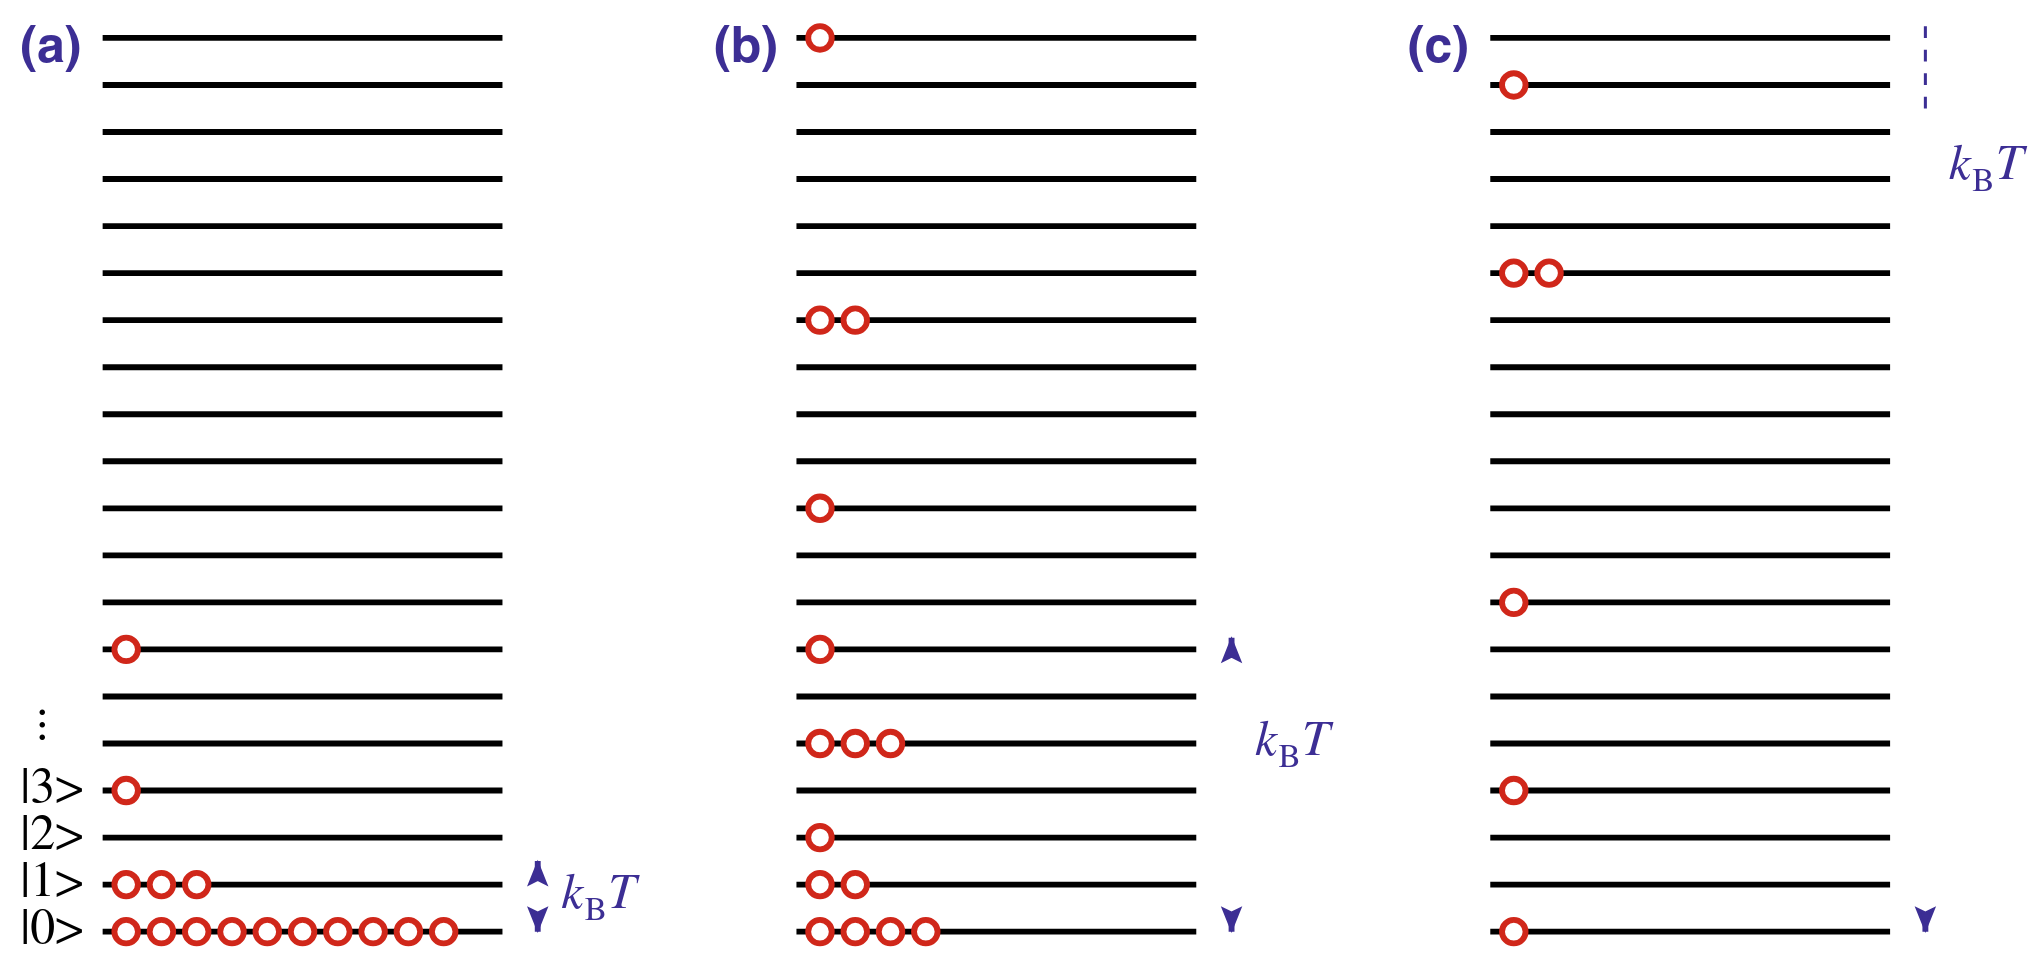
\includegraphics[width = 0.70 \textwidth]{ideal-high-temp.png}
	\caption{Occupancies of single-particle energy eigenstates for a bosonic system in the low-, intermediate- and high-temperature limits.}
	\label{boson-temp}
\end{figure}

\subsection{Limite ad alta temperatura}

Nel limite ad alta temperatura si può non tenere conto dell'occupazione degli stati, poiché il gas si comporta classicamente e $ n_\alpha \in \{0,1\} \,\,\forall \alpha \in \mathcal{I} $. Si ottiene dunque una funzione di partizione ad alta temperatura valida sia per fermioni che per bosoni:
\begin{equation}
	Z \simeq \frac{1}{N!} \sum_{\alpha_1, \dots, \alpha_N \in \mathcal{I}} \exp \left( -\beta \sum_{i = 1}^N E_{\alpha_i} \right) = \frac{1}{N!} \prod_{i = 1}^N Z_i \equiv \frac{Z_1^N}{N!}
\end{equation}
dove $ Z_1 $ è la funzione di partizione single-particle $ Z_1 \equiv \sum_{\alpha \in \mathcal{I}} \exp \left( -\beta E_\alpha \right) $. \\
Essendo in fase gassosa, il centro di massa di ciascuna particella si muove liberamente ed è dunque separabile dai gradi di libertà interni, ovvero $ \mathcal{H}_i = \mathcal{H}_{i,\text{tr}} + \mathcal{H}_{i,\text{int}} $ e $ Z_1 = Z_{1,\text{tr}} Z_{1,\text{int}} $: mentre $ Z_{1,\text{int}} $ dipende dallo specifico spettro di eccitazioni dei gradi di libertà interni, $ Z_{1,\text{tr}} $ è universale e dipende solo dalla massa della particella $ M $ e dal volume in cui si trova il sistema $ V $.

\subsubsection{Gradi di libertà traslazionali}

Si consideri una particella confinata in un cubo macroscopico di volume $ V = L^3 $ e si impongano delle condizioni al contorno periodiche, ovvero che la funzione d'onda sia uguale su facce opposte del cubo. Le autofunzioni $ \psi_\ve{k}(\ve{r}) = L^{-3/2} \exp(i \ve{k} \cdot \ve{r}) $ possono avere solo valori quantizzati di $ \ve{k} $:
\begin{equation*}
	k_j = \frac{2\pi}{L} n_j \,\,,\,\, n_j \in \Z
\end{equation*}
L'energia cinetica traslazionale associata è:
\begin{equation}
	E_\ve{n} = \frac{\hbar^2 \ve{k}^2}{2M} = \frac{(2\pi\hbar)^2}{2M L^2} (n_x^2 + n_y^2 + n_z^2)
\end{equation}
Per $ L $ o $ M $ macroscopicamente grande (limite termodinamico) questo spettro diventa continuo:
\begin{equation*}
	\begin{split}
		Z_{1,\text{tr}}
		& = \sum_{\ve{n} \in \Z^3} e^{-\beta E_\ve{n}} = \sum_{\ve{n} \in \Z^3} \exp \left[ - \beta \frac{(2\pi\hbar)^2}{2M L^2} (n_x^2 + n_y^2 + n_z^2) \right] \\
		& \rightarrow \int_{\R^3} \dd n_x \dd n_y \dd n_z \exp \left[ -\beta \frac{(2\pi\hbar)^2}{2M L^2} (n_x^2 + n_y^2 + n_z^2) \right] = \left( \frac{L}{\hbar} \sqrt{\frac{M k_\text{B} T}{2\pi}} \right)^3
	\end{split}
\end{equation*}
Si può definire la \textit{lunghezza termica}:
\begin{equation}
	\Lambda \defeq \sqrt{\frac{2\pi\hbar^2}{M k_\text{B} T}}
\end{equation}
così da ottenere:
\begin{equation}
	Z_{1,\text{tr}} = \frac{V}{\Lambda^3}
\end{equation}
Si ha dunque:
\begin{equation*}
	Z = \frac{Z_1^N}{N!} = \frac{Z_{1,\text{tr}}^N}{N!} Z_{1,\text{int}}^N \equiv Z_\text{tr} Z_{1,\text{int}}^N
\end{equation*}

\begin{proposition}[before upper = {\tcbtitle}]{Energia interna traslazionale}{}
	\begin{equation}
		U_\text{tr} = \frac{3}{2} N k_\text{B} T
	\end{equation}

	\tcblower

	\begin{proof}
		\begin{equation*}
			\begin{split}
				U_\text{tr}
				& = - \frac{\pa}{\pa \beta} \ln Z_\text{tr} = - \frac{\pa}{\pa \beta} \ln \frac{V^N}{N! \Lambda^{3N}} = 3N \frac{\pa}{\pa \beta} \ln \Lambda = 3N \frac{\pa}{\pa \beta} \ln \sqrt{\beta} = \frac{3N}{2\beta} = \frac{3}{2} N k_\text{B} T
			\end{split}
		\end{equation*}
	\end{proof}
\end{proposition}

Ciò è in accordo con l'equipartizione dell'energia di Boltzmann.

\begin{theorem}{Equazione di stato dei gas perfetti}{}
	Per un gas perfetto vale l'equazione di stato:
	\begin{equation}
		P = \frac{N k_\text{B} T}{V}
	\end{equation}

	\tcblower

	\begin{proof}
		Innanzitutto, si trova l'energia libera nel limite ad alta temperatura:
		\begin{equation*}
			F \defeq - \frac{\ln Z}{\beta} \simeq - \frac{1}{\beta} \ln \frac{(Z_1)^N}{N!} = - \frac{1}{\beta} (N \ln Z_1 - \ln N!) \simeq - \frac{1}{\beta} (N \ln Z_1 - N \ln (N/e))
		\end{equation*}
		dove si è usata l'approssimazione di Stirling $ \ln N! \simeq N \ln (N/e) $. Dunque:
		\begin{equation}
			F = - N k_\text{B} T \ln \frac{e Z_1}{N}
		\end{equation}
		Per la pressione:
		\begin{equation*}
			\begin{split}
				P \defeq - \frac{\pa F}{\pa V} \bigg\vert_{T,N}
				& = - \frac{\pa}{\pa V} \bigg\vert_{T,N} \left[ - N k_\text{B} T \ln \frac{e Z_{1,\text{tr}} Z_{1,\text{int}}}{N} \right] = N k_\text{B} T \frac{\pa}{\pa V} \bigg\vert_{T,N} \left[ \ln \frac{eV}{N \Lambda^3} + \ln Z_{1,\text{int}} \right] \\
				& = N k_\text{B} T \frac{\pa}{\pa V}\bigg\vert_{T,N} \ln \frac{eV}{N \Lambda^3} = N k_\text{B} T \frac{1}{V}
			\end{split}
		\end{equation*}
	\end{proof}
\end{theorem}

Confrontando con $ pV = nRT $, essendo $ N = n N_\text{A} $, si trova $ k_\text{B} = R / N_\text{A} $.

\paragraph{Distribuzione energetica}

Per ricavare la distribuzione di Boltzmann delle energie cinetiche è necessario passare da un'integrale sugli stati $ \ve{n} $ ad un'integrale sull'energia $ E $. La densità degli stati nello spazio degli stati è:
\begin{equation}
	g(\ve{k}) = \frac{\dd n_x}{\dd k_x} \frac{\dd n_y}{\dd k_y} \frac{\dd n_z}{\dd k_z} = \frac{L^3}{8\pi^3} \equiv \frac{V}{8\pi^3}
	\label{eq:dens-k}
\end{equation}
Si vede che gli stati sono distribuiti uniformemente. È necessario trovare la densità degli stati nello spazio delle energie tale per cui:
\begin{equation*}
	g(E) \dd E = g(\ve{k}) \dd^3\ve{k} = g(\ve{k}) 4\pi k^2 \dd k
\end{equation*}
Il differenziale $ \dd k $ si ottiene invertendo la relazione di dispersione $ E = E(k) $, che in questo caso dà:
\begin{equation*}
	k = \sqrt{\frac{2M E}{\hbar^2}}
	\quad \Rightarrow \quad
	\dd k = \sqrt{\frac{M}{2\hbar^2 E}} \dd E
\end{equation*}
Si ottiene dunque:
\begin{equation*}
	g(E) \dd E = \frac{V}{8\pi^3} 4 \pi \frac{2M E}{\hbar^2} \sqrt{\frac{M}{2\hbar^2 E}} \dd E = \frac{V M^{3/2}}{\sqrt{2} \pi^2 \hbar^3} \sqrt{E} \dd E
\end{equation*}
ovvero:
\begin{equation}
	g_\text{tr}(E) = \frac{V M^{3/2}}{\sqrt{2} \pi^2 \hbar^3} \sqrt{E}
	\label{eq:en-deg}
\end{equation}
La distribuzione di probabilità che descrive l'energia di una singola particella si può trovare come:
\begin{equation*}
	\frac{\dd P(E)}{\dd E} = g_\text{tr}(E) \frac{e^{- \beta E}}{Z_{1,\text{tr}}} = \frac{V M^{3/2}}{\sqrt{2} \pi^2 \hbar^3} \sqrt{E} \frac{\Lambda^3}{V} e^{-\beta E}
\end{equation*}
Il risultato è indipendente dal volume e dalla massa della particella, ed è dunque universale (a parità di temperatura):
\begin{equation}
	\frac{\dd P(E)}{\dd E} = \frac{2}{\sqrt{\pi}} \beta^{3/2} \sqrt{E} e^{-\beta E}
	\label{eq:maxw-boltz-en}
\end{equation}
Si può ricavare anche una distribuzione delle velocità, trovando che ciascuna componente di $ \ve{v} = \frac{\ve{p}}{M} $ è distribuita gaussianamente come:
\begin{equation*}
	\frac{\dd P(v_j)}{\dd v_j} = \sqrt{\frac{\beta M}{2\pi}} \exp \left( -\beta \frac{M v_j^2}{2} \right)
\end{equation*}
La distribuzione di $ v \equiv \abs{\ve{v}} $ si trova dall'Eq. \ref{eq:maxw-boltz-en}:
\begin{equation*}
	\frac{\dd P(v)}{\dd v} = \frac{\dd P(E)}{\dd E} \frac{\dd E}{\dd v} = M v \frac{\dd P(E)}{\dd E}
\end{equation*}
Sostituendo $ E = \frac{1}{2} M v^2 $ si trova la \textit{distribuzione di Maxwell-Boltzmann}:
\begin{equation}
	\frac{\dd P(v)}{\dd v} = \sqrt{\frac{2 M^3}{\pi (k_\text{B} T)^3}} v^2 \exp \left( - \frac{M}{2 k_\text{B} T} v^2 \right)
\end{equation}

\subsubsection{Gradi di libertà interni}

Per quanto riguarda $ \mathcal{H}_{i,\text{int}} $, si può assumere una separazione netta tra i gradi di libertà rotazionali e quelli vibrazionali (al pari delle molecole), così da poter scrivere $ \mathcal{H}_{i,\text{int}} = \mathcal{H}_{i,\text{vib}} + \mathcal{H}_{i,\text{rot}} $ e dunque $ Z_{1,\text{int}} = Z_{1,\text{vib}} Z_{1,\text{rot}} $.

\paragraph{Componente vibrazionale}

Addottando l'approssimazione armonica, l'Hamiltoniana vibrazionale si riduce a quella di oscillatore armonico $ E_{1,\text{vib}} = \hbar \omega \left( v + \frac{1}{2} \right) $, con $ \omega \defeq\sqrt{\kappa / \mu} $ e $ \kappa \equiv \frac{\pa^2 V_\text{ad}}{\pa R^2}\vert_{R = R_\text{m}} $.

\begin{proposition}{Funzione di partizione vibrazionale}{}
	Definendo $ x \equiv \theta_\text{vib} / T $, si ha:
	\begin{equation}
		Z_{1,\text{vib}} = \frac{1}{2 \sinh(x/2)}
	\end{equation}

	\tcblower

	\begin{proof}
		\begin{equation*}
			Z_{1,\text{vib}} = \sum_{v \in \N_0} \exp \left[ -\beta \hbar \omega \left( v + \frac{1}{2} \right) \right] = \exp \left( - \frac{x}{2} \right) \sum_{v = 0}^\infty \exp \left( -v x \right) = \frac{e^{-x/2}}{1 - e^{-x}} = \frac{1}{2 \sinh(x/2)}
		\end{equation*}
	\end{proof}
\end{proposition}

Dall'Eqq. \ref{eq:int-en-z}-\ref{eq:cal-spec-z} si ricavano:
\begin{equation}
	U_{1,\text{vib}} = \hbar \omega \left( \frac{1}{2} + \frac{1}{e^x - 1} \right)
\end{equation}
\begin{equation}
	c_{V,1,\text{vib}} = k_\text{B} \left[ \frac{x/2}{\sinh(x/2)} \right]^2
\end{equation}
Si ricordi che, in quanto grandezze estensive, $ U_\text{vib} = N U_{1,\text{vib}} $ e $ c_{V,\text{vib}} = N c_{V,1,\text{vib}} $. Gli andamenti di queste quantità sono riportati in Fig. \ref{vib-heat-int}: si vede che $ U_{1,\text{vib}} $ è asintoticamente lineare in $ T $ (come ci si aspetterebbe, contibuendo per $ 2 \cdot \frac{1}{2} k_\text{B} T $ all'energia interna totale), ed anche $ c_{V,1,\text{vib}} $ tende asintoticamente al suo valore classico. Questo comportamente è detto $ \virgolette{scongelamento} $ dei gradi di libertà rotazionali ed avviene una volta superata la soglia $ \theta_\text{vib} \sim 10^3-10^4 \,\text{K} $.

\begin{figure}
	\centering
	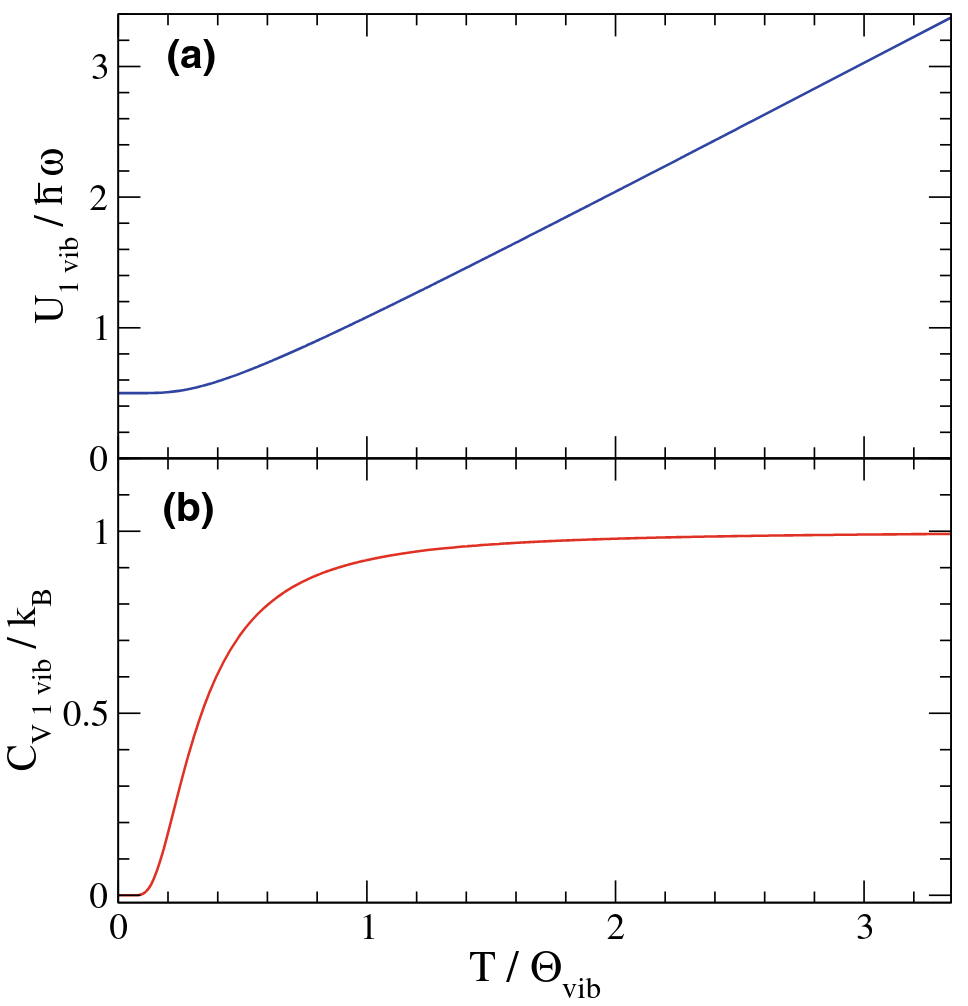
\includegraphics[width = 0.50 \textwidth]{vib-heat-int.png}
	\caption{Temperature dependence of $ U_{1,\text{vib}} $ and $ c_{V,1,\text{vib}} $.}
	\label{vib-heat-int}
\end{figure}

\paragraph{Componente rotazionale}

Nell'approssimazione di rotatore rigido libero, la funzione d'onda rotazionale è un'armonica sferica e lo spettro energetico è $ E_\text{rot} = \frac{\hbar^2}{2I} \ell (\ell + 1) $, con $ I \equiv \mu R_\text{m}^2 $. In questo caso non c'è una forma analitica compatta:
\begin{equation*}
	Z_{1,\text{rot}} = \sum_{\ell \in \N_0} \sum_{m = -\ell}^{\ell} e^{- \frac{\beta \hbar^2}{2I} \ell (\ell + 1)} = \sum_{\ell = 0}^\infty (2\ell + 1) \exp \left[ -\frac{\theta_\text{rot}}{T} \ell (\ell + 1) \right]
\end{equation*}
La temperatura caratteristica $ \theta_\text{rot} $ è tendenzialmente molto bassa ($ \sim 1-10 \,\text{K} $, la più alta è $ 85 \,\text{K} $ per $ \ch{H_2} $), dunque, dato che nel regime $ \theta_\text{rot} / T \ll 1 $ l'esponenziale decade lentamente e molti termini contribuiscono a $ Z_{1,\text{rot}} $, si può approssimare:
\begin{equation*}
	Z_{1,\text{rot}} \simeq \int_0^\infty \dd\ell\, (2\ell + 1) \exp \left[ - \frac{\theta_\text{rot}}{T} \ell (\ell + 1) \right] = \int_0^\infty \dd y\, e^{- \frac{\theta_\text{rot}}{T} y}
\end{equation*}
Si trova quindi che, per $ T \gg \theta_\text{rot} $:
\begin{equation}
	Z_{1,\text{rot}} \simeq \frac{T}{\theta_\text{rot}}
\end{equation}
Dall'Eqq. \ref{eq:int-en-z}-\ref{eq:cal-spec-z} si ricavano:
\begin{equation}
	U_{1,\text{rot}} \simeq k_\text{B} T
\end{equation}
\begin{equation}
	c_{V,1,\text{rot}} \simeq k_\text{B}
\end{equation}
che sono proprio i valori classicamente attesi (confermando il limite ad alta temperatura come il limite classico con $ \virgolette{scongelamento} $ dei gradi di libertà interni). Per $ T \ll \theta_\text{rot} $, invece, l'esponenziale decade velocemente e $ Z_{1,\text{rot}} $ è ottenuto troncando la serie ai primi termini (tendenzialmente si tengono $ \ell = 0 $ e $ \ell = 1 $): l'andamento a tutte le temperature è riportato in Fig. \ref{rot-heat-int}. \\
L'espanzione in serie di $ Z_{1,\text{rot}} $ fornisce anche un metodo quantitativo per calcolare le intensità relative dei picchi di uno spettro roto-vibrazionale, poiché dà la probabilità di occupazione di un livello $ (\ell,m) $ o complessivamente $ \ell $:
\begin{equation}
	P_{\ell,m} = \frac{e^{- \frac{\beta \hbar^2}{2I} \ell (\ell + 1)}}{Z}
	\qquad \qquad
	P_\ell = \frac{2\ell + 1}{Z} e^{- \frac{\theta_\text{rot}}{T} \ell (\ell + 1)}
\end{equation}

\begin{proposition}{}{}
	La riga più intensa in uno spettro roto-vibrazionale è quella associata a $ \ell_\text{max} \rightarrow \ell_\text{max} \pm 1 $, con:
	\begin{equation}
		\ell_\text{max} = \frac{1}{2} \left[ \sqrt{\frac{2T}{\theta_\text{rot}}} - 1 \right]
	\end{equation}

	\tcblower

	\begin{proof}
		La riga più intensa è quella associata al livello rotazionale più popolato. Quest'ultimo si trova ponendo:
		\begin{equation*}
			\frac{\dd P_\ell}{\dd \ell}\bigg\vert_{\ell = \ell_\text{max}} = 0
			\quad \Rightarrow \quad
			2 - (2 \ell_\text{max} + 1)^2 \frac{\theta_\text{rot}}{T} = 0
			\quad \Rightarrow \quad
			\ell_\text{max} = \frac{1}{2} \left[ \sqrt{\frac{2T}{\theta_\text{rot}}} - 1 \right]
		\end{equation*}
	\end{proof}
\end{proposition}

\begin{figure}
	\centering
	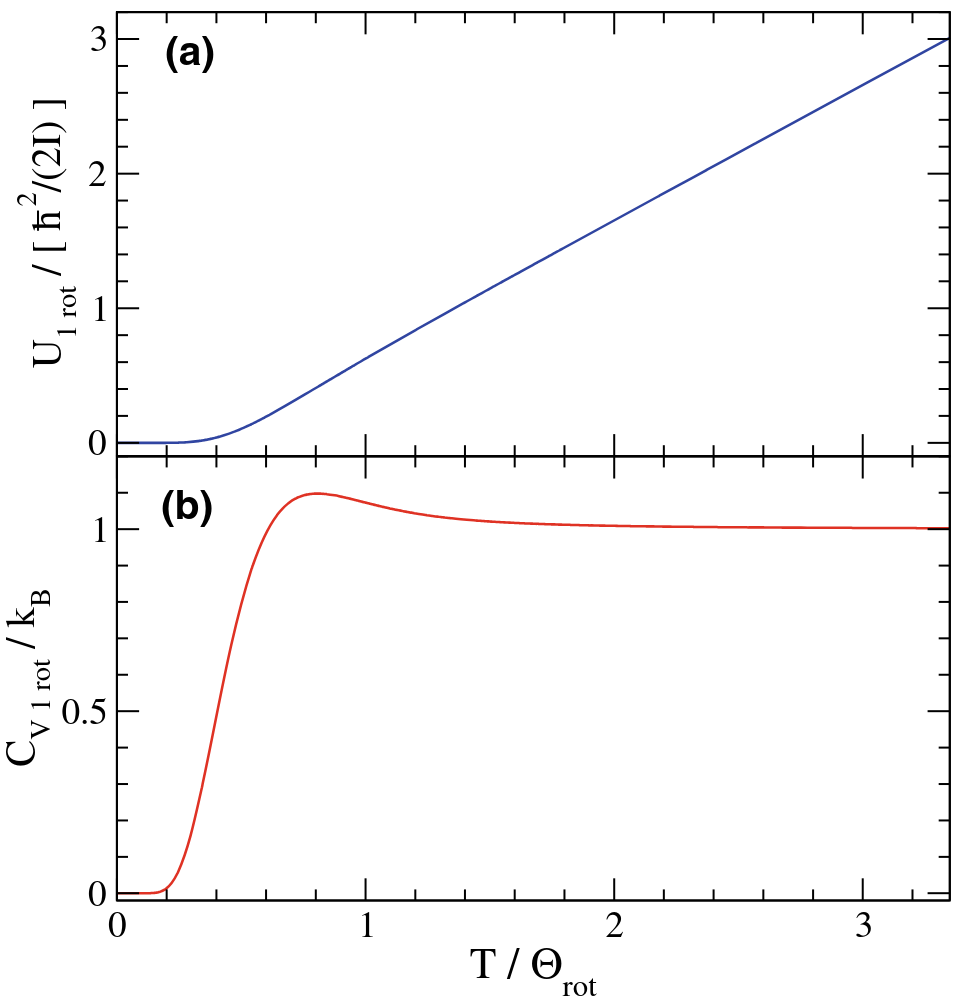
\includegraphics[width = 0.50 \textwidth]{rot-heat-int.png}
	\caption{Temperature dependence of $ U_{1,\text{vib}} $ and $ c_{V,1,\text{vib}} $.}
	\label{rot-heat-int}
\end{figure}

\paragraph{Calore specifico totale}

Mettendo insieme il contributo rotazionale e quello vibrazionale al calore specifico, si ottiene l'andamento in Fig. \ref{vib-rot-c}: a $ T = 0 \,\text{K} $ è presente il solo contributo traslazionale, mentre aumentando la temperatura si scongelano prima i gradi di libertà rotazionali e poi, a temperature sufficientemente elevate, quelli vibrazionali.

\begin{figure}
	\centering
	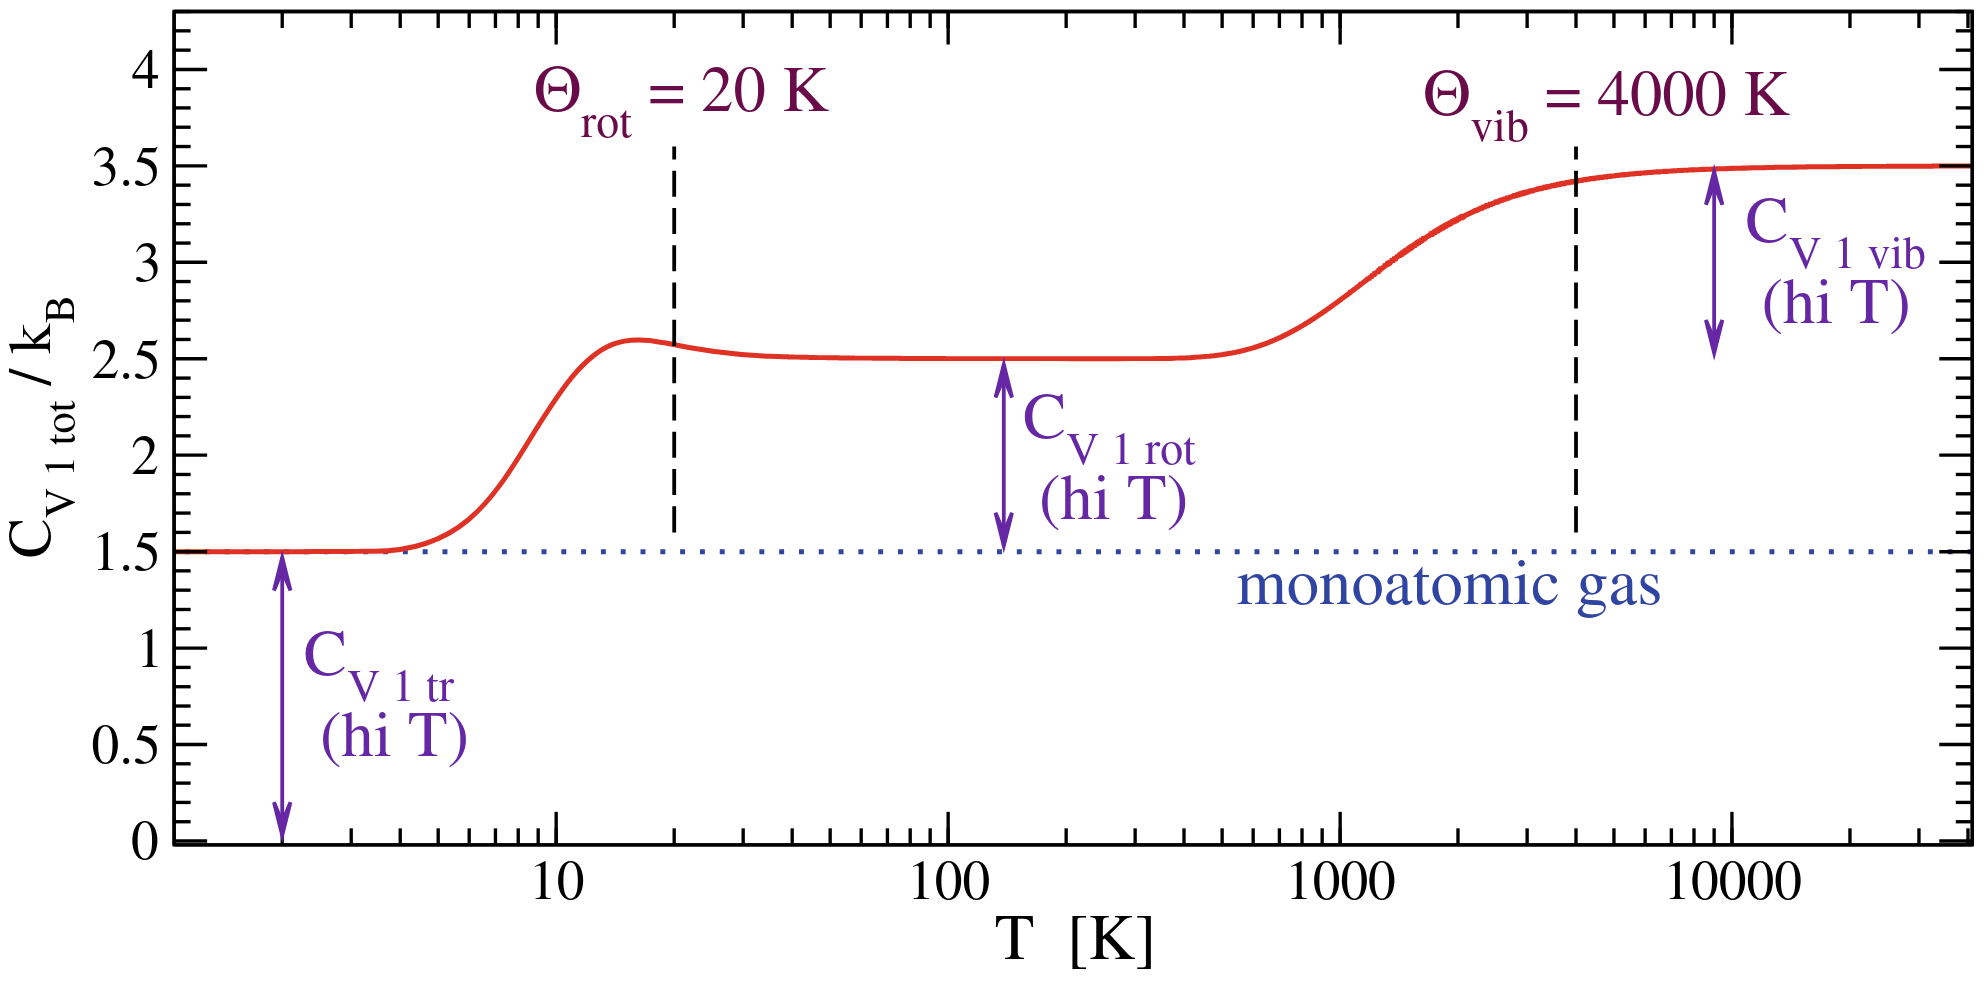
\includegraphics[width = 0.80 \textwidth]{vib-rot-c.png}
	\caption{Temperature dependence of $ c_{V,1} = c_{V,1,\text{tr}} + c_{V,1,\text{rot}} + c_{V,1,\text{vib}} $ for biatomic molecules.}
	\label{vib-rot-c}
\end{figure}

\subsection{Limite a bassa temperatura}

Mentre ad alte temperature sia i sistemi fermionici che quelli bosonici si comportano come dei gas ideali classici, a basse temperature il loro comportamento diverge a causa dei differenti vincoli sull'occupazione dei livelli energetici. \\
Riscrivendo l'Eq. \ref{eq:z-sing-part} rispetto ai numeri d'occupazione (quindi abbandonando la descrizione rispetto alle singole particelle):
\begin{equation}
	Z = \sum_{\alpha_1, \dots, \alpha_N \in \mathcal{I}} \frac{\prod_{k \in \mathcal{I}} n_k!}{N!} \exp \left( -\beta \sum_{i = 1}^N E_{\alpha_i} \right) = \sum_{\{n_\alpha\}} \prod_{\alpha \in \mathcal{I}} \left( e^{-\beta E_\alpha} \right)^{n_\alpha}
	\label{eq:z-n-occ}
\end{equation}
dove $ \{n_\alpha\} \equiv \{n_\alpha \in \mathcal{N}, \alpha \in \mathcal{I} : \sum_{\alpha \in \mathcal{I}} n_\alpha = N\} $, con $ \mathcal{N} = \{0,1\} $ per fermioni e $ \mathcal{N} = \N_0 $ per bosoni. Il vincolo $ \sum_{\alpha \in \mathcal{I}} n_\alpha = N $ rende impossibile dare una forma esplicita a tale sommatoria: per ovviare al problema si introduce un nuovo ensemble, l'\textit{ensemble gran-canonico}, il quale scambia debolmente con l'ambiente non solo energia ma anche particelle. Per mantenere costante e pari a $ N $ il numero medio di particelle, ovvero $ [\hat{N}] = N $, si aggiunge un termine all'autovalore energetico, ottenendo la \textit{funzione di gran-partizione}:
\begin{equation}
	Q \defeq \sum_{N = 0}^\infty \sum_{m(N)} e^{- \beta (E_{m(N)} - \mu N)} \equiv \sum_{N = 0}^\infty \tr e^{- \beta (\mathcal{H} - \mu \hat{N})}
\end{equation}
dove la seconda sommatoria è su tutti gli autostati $ \ket{m(N)} $ di un sistema a $ N $ particelle e $ \mu $ è il potenziale chimico. Essendo $ E_{m(N)} $ una funzione crescente in $ N $, l'esponente $ E_{m(N)} - \mu N $ avrà un minimo per un certo $ N $. Il numero medio di particelle risulta essere:
\begin{equation*}
	[\hat{N}] = \frac{1}{Q} \sum_{N = 0}^\infty \sum_{m(N)} N e^{-\beta (E_{m(N)} - \mu N)} = \frac{1}{\beta} \frac{\pa}{\pa \mu} \ln Q
\end{equation*}

\begin{definition}[before upper = {\tcbtitle}]{Potenziale gran-canonico}{}
	\begin{equation}
		\Omega \defeq - \frac{1}{\beta} \ln Q = - PV
	\end{equation}
\end{definition}

\begin{proposition}{Quantità termodinamiche}{gran-canon-term}
	Si trovano le seguenti relazioni\footnote{L'energia intera si trova da $ U = F + TS $.}:
	\begin{itemize}
		\item numero medio di particelle $ [\hat{N}] = - \frac{\pa \Omega}{\pa \mu}\big\vert_{T,V} $;
		\item entropia $ S = - \frac{\pa \Omega}{\pa T}\big\vert_{\mu,V} $;
		\item energia libera $ F = \Omega + \mu [\hat{N}] $;
		\item potenziale di Gibbs $ G = \mu [\hat{N}] $;
	\end{itemize}
\end{proposition}

Si può calcolare esplicitamente la funzione di gran-partizione per un sistema di bosoni/fermioni non-interagenti.

\begin{theorem}{Gran-partizioni ideali}{}
	Per un sistema di bosoni/fermioni non-interagenti si ha:
	\begin{equation}
		Q = \prod_{\alpha \in \mathcal{I}} \left( 1 - \theta e^{\beta (\mu - E_\alpha)} \right)^{-\theta}
	\end{equation}
	dove $ \theta = +1 $ per sistemi bosonici e $ \theta = -1 $ per sistemi fermionici.

	\tcblower

	\begin{proof}
		Rielaborando l'Eq. \ref{eq:z-n-occ}:
		\begin{equation*}
			\begin{split}
				Q
				& = \sum_{N = 0}^\infty \sum_{\{n_\alpha\}} e^{-\beta ( \sum_{\alpha \in \mathcal{I}} n_\alpha E_\alpha - \mu N)} = \sum_{N = 0}^\infty \sum_{\{n_\alpha\}} e^{-\beta \sum_{\alpha \in \mathcal{I}} n_\alpha (E_\alpha - \mu)} \\
				& = \sum_{n_\alpha \in \mathcal{N}} \prod_{\alpha \in \mathcal{I}} e^{\beta (\mu - E_\alpha) n_\alpha} = \prod_{\alpha \in \mathcal{I}} \sum_{n_\alpha \in \mathcal{N}} \left( e^{\beta (\mu - E_\alpha)} \right)^{n_\alpha}
			\end{split}
		\end{equation*}
		Per fermioni $ \mathcal{N} \equiv \{0,1\} $, quindi:
		\begin{equation*}
			Q = \prod_{\alpha \in \mathcal{I}} \left( 1 + e^{\beta (\mu - E_\alpha)} \right)
		\end{equation*}
		Per bosoni $ \mathcal{N} \equiv \N_0 $, quindi\footnote{Perché la serie geometria coverga, bisogna avere $ \mu - E_\alpha < 0 $, ovvero $ \mu < E_\alpha \,\,\forall \alpha \in \mathcal{I} $. Tipicamente l'energia minima è $ E_\text{min} = 0 $, dunque il potenziale chimico per i bosoni deve essere negativo}:
		\begin{equation*}
			Q = \prod_{\alpha \in \mathcal{I}} \frac{1}{1 - e^{\beta (\mu - E_\alpha)}}
		\end{equation*}
		Definendo il parametro $ \theta $ si ottiene la tesi.
	\end{proof}
\end{theorem}

\begin{theorem}{Statistiche quantistiche}{}
	Per un sistema di bosoni/fermioni non-interagenti si ha:
	\begin{equation}
		[n_\alpha] = \frac{1}{e^{\beta (E_\alpha - \mu)} - \theta}
		\label{eq:fer-dir-bos-ein}
	\end{equation}
	dove $ \theta = +1 $ per sistemi bosonici e $ \theta = -1 $ per sistemi fermionici.

	\tcblower

	\begin{proof}
		Usando la Prop. \ref{prop:gran-canon-term}:
		\begin{equation*}
			\begin{split}
				[\hat{N}]
				& = \frac{1}{\beta} \frac{\pa}{\pa \mu} \ln Q = \frac{1}{\beta} \frac{\pa}{\pa \mu} \sum_{\alpha \in \mathcal{I}} -\theta \ln \left( 1 - \theta e^{\beta (\mu - E_\alpha)} \right) \\
				& = - \frac{\theta}{\beta} \sum_{\alpha \in \mathcal{I}} \frac{-\theta \beta e^{\beta (\mu - E_\alpha)}}{1 - \theta e^{\beta (\mu - E_\alpha)}} = \sum_{\alpha \in \mathcal{I}} \frac{1}{e^{\beta (E_\alpha - \mu)} - \theta}
			\end{split}
		\end{equation*}
		Dato che $ [\hat{N}] = \sum_{\alpha \in \mathcal{I}} [n_\alpha] $ si trova la tesi.
	\end{proof}
\end{theorem}

Queste sono le distribuzioni di Bose-Einstein (bosoni) e Fermi-Dirac (fermioni). Si vede che a $ T $ e $ \mu $ fissati, l'occupazione media di uno stato è determinato esclusivamente dalla sua energia\footnotemark. Inoltre, la presenza di altre particelle influenza l'occupazione media di uno stato tramite il potenziale chimico $ \mu $, il quale è funzione della densità totale media $ [\hat{N}]/V $ e della temperatura $ T $.
%
\footnotetext{In particolare, in assenza di campi magnetici esterni, $ [n_\alpha] $ è indipendente da $ m_s $: di conseguenza, gas ideali di bosoni/fermioni rimangono in uno stato complessivo non-magnetizzato e non-polarizzato a qualsiasi temperatura.}
%
Si noti che giustamente $ [n_\alpha]_\text{Fermi} \in [0,1] $ e che entrambe, per $ E_\alpha \gg \mu $, possono essere approssimate da $ [n_\alpha] \approx e^{-\beta (E_\alpha - \mu)} $, ovvero una distribuzione di Boltzmann (limite classico\footnotemark, opposto al limite degenere a bassa temperatura).

\footnotetext{Considerando un gas perfettamente ideale, ovvero non-interagente, allora se esso venisse preparato in uno stato iniziale lontano dall'equilibrio non raggiungerebbe mai quest'ultimo, in quanto è necessaria un'interazione almeno con l'ambiente.}

\subsubsection{Fermioni}

\begin{figure}
	\centering
	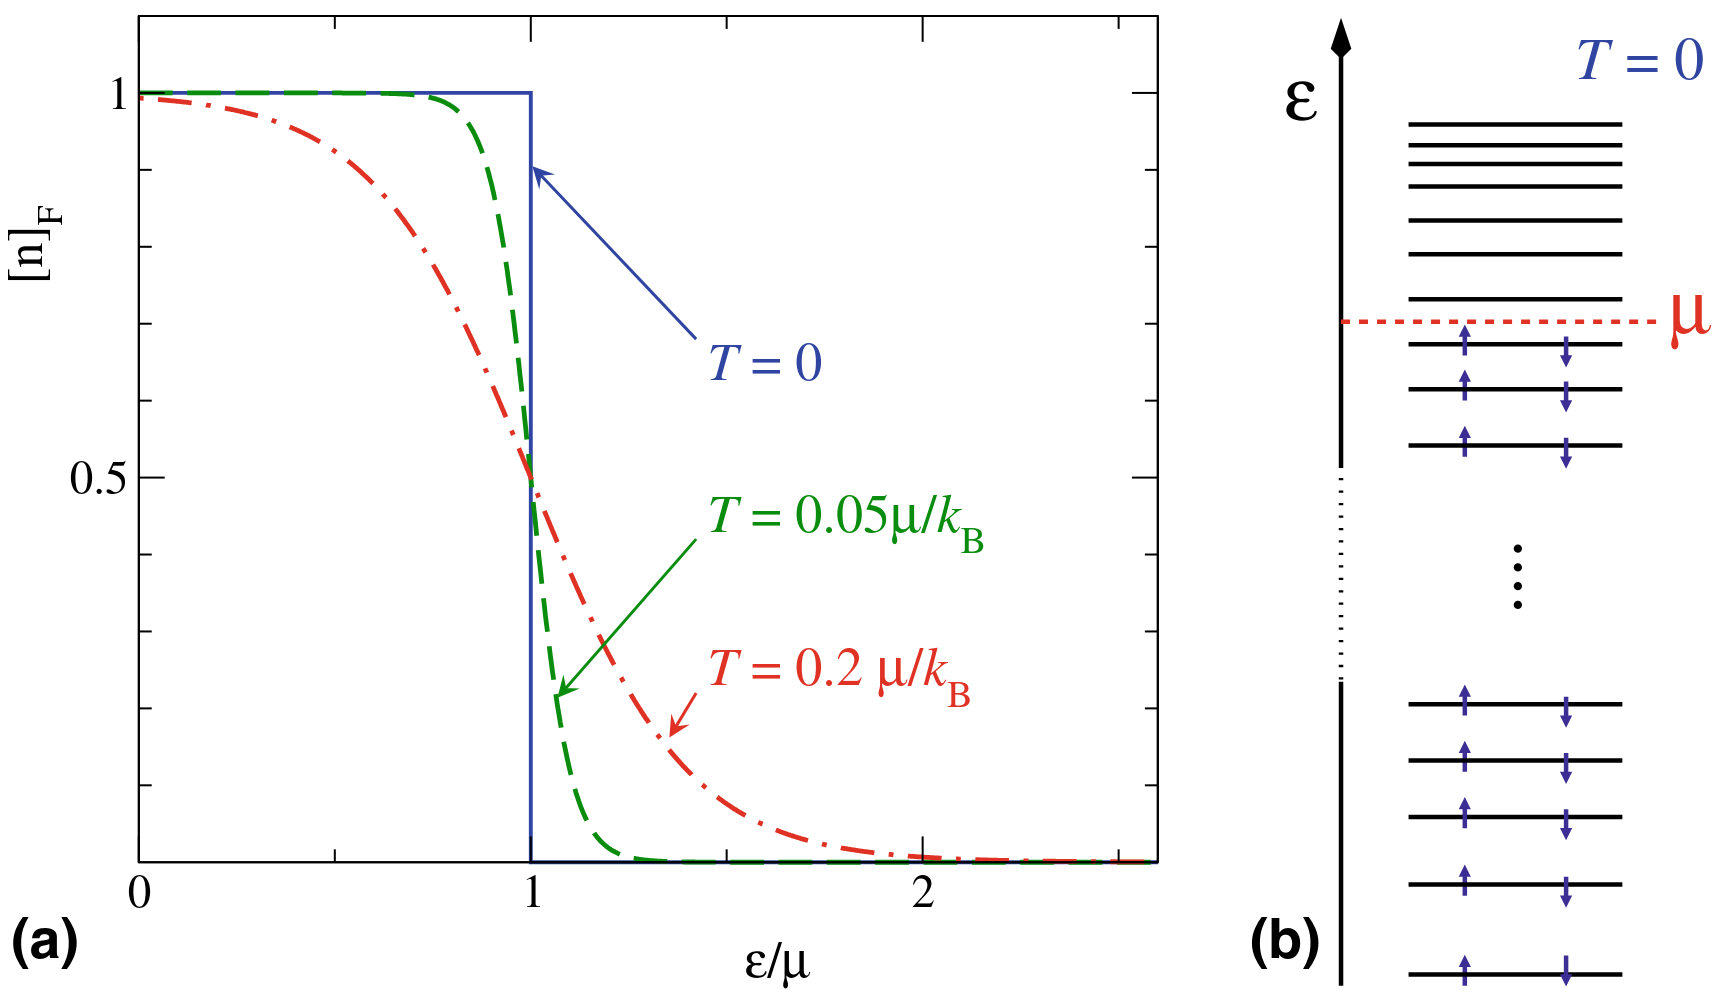
\includegraphics[width = 0.50 \textwidth]{fermi-distr.png}
	\caption{Fermi distribution at various temperatures and filling of single-particle states.}
	\label{fermi-distr}
\end{figure}

Come si vede in Fig. \ref{fermi-distr}, per a $ T = 0 \,\text{K} $ la distribuzione di Fermi-Dirac diventa una funzione a gradino. A questa temperatura, il comportamento del gas di Femi è quello del ground state di un sistema di $ N \equiv [\hat{N}] $ fermioni liberi non-interagenti: questo è ottenuto antisimmetrizzando gli stati in cui vengono riempiti gli $ N $ livelli energetici single-particle con energia più bassa, fino ad un'energia massima $ \varepsilon_\text{F} $ detta \textit{energia di Fermi}.

\begin{theorem}{Energia di Fermi}{}
	L'energia di Fermi è:
	\begin{equation}
		\varepsilon_\text{F} \equiv \mu(T = 0) = \frac{\hbar^2}{2M} \left( \frac{6\pi^2}{g_s} \frac{N}{V} \right)^{2/3}
	\end{equation}
	dove $ g_s $ è la degenerazione da spin dei livelli energetici single-particle.

	\tcblower

	\begin{proof}
		Si noti che, ponendo $ \mu \equiv \mu(T = 0) $:
		\begin{equation*}
			\lim_{T \rightarrow 0} [n_\alpha]_\text{F} =
			\begin{cases}
				1 & E_\alpha < \mu \\
				\frac{1}{2} & E_\alpha = \mu \\
				0 & E_\alpha > \mu
			\end{cases}
		\end{equation*}
		Ricordando l'Eq. \ref{eq:en-deg}:
		\begin{equation*}
			N \equiv [\hat{N}] = \int_0^\infty \dd E\, g(E) [n_\alpha]_\text{F} = \int_0^\mu \dd E\, g(E) = g_s \frac{V M^{3/2}}{\sqrt{2} \pi^2 \hbar^3} \int_0^\mu \dd E\, \sqrt{E} = \frac{(2M)^{3/2} V g_s}{4\pi^2 \hbar^3} \frac{2}{3} \mu^{3/2}
		\end{equation*}
		Risolvendo per $ \mu $ e contando che $ \varepsilon_\text{F} \equiv \mu $ si ha la tesi.
	\end{proof}
\end{theorem}

Passando allo spazio dei momenti, si trova il \textit{momento di Fermi}:
\begin{equation}
	k_\text{F} = \sqrt[3]{\frac{6\pi^2}{g_s} \frac{N}{V}}
	\label{eq:k-f}
\end{equation}
che è concorde con $ N = \frac{4}{3} \pi k_\text{F}^3 \cdot g_s \cdot \frac{V}{8\pi^3} $ (volume $ \cdot $ degenerazione $ \cdot $ densità nello spazio dei momenti).

\begin{example}{Gas di elettroni liberi}{}
	Un esempio di gas di Fermi è l'insieme degli elettroni di conduzione di un metallo, che è un gas di elettroni liberi: per esso $ \frac{N}{V} \sim 10^{29}-10^{30} \,\text{m}^{-3} $, quindi $ k_\text{F} \sim 10^{10} \,\text{m}^{-1} $ ($ v_\text{F} \sim 10^6 \,\text{m}/\text{s} $) e $ \varepsilon_\text{F} \sim 5-10 \ev $.
\end{example}

\begin{proposition}{Energia interna}{}
	A $ T = 0 $ l'energia interna di un gas di Fermi è:
	\begin{equation}
		U(T = 0) = \frac{3}{5} N \varepsilon_\text{F}
	\end{equation}

	\tcblower

	\begin{proof}
		Per calcolo diretto:
		\begin{equation*}
			U(T = 0) = \int_0^\infty \dd E\, E g(E) [n_\alpha]_\text{F} = \int_0^\mu \dd E\, E g(E) = \frac{(2M)^{3/2} V g_s}{4\pi^2 \hbar^3} \frac{2}{5} \varepsilon_\text{F}^{5/2} = \frac{3}{5} N \varepsilon_\text{F}
		\end{equation*}
	\end{proof}
\end{proposition}

Si vede quindi che l'energia interna media per elettrone $ \frac{U}{N} = \frac{3}{5} \varepsilon_\text{F} $ non va a zero per $ T \rightarrow 0 $: questa è una conseguenza del principio di Pauli.

\begin{proposition}{Pressione}{}
	A $ T = 0 $ la pressione di un gas di Fermi è:
	\begin{equation}
		P(T = 0) = \frac{2}{3} \frac{U}{V}
	\end{equation}

	\tcblower

	\begin{proof}
		A $ T = 0 $ si ha $ U = F $, quindi:
		\begin{equation*}
			\begin{split}
				P
				& \defeq - \frac{\pa F}{\pa V}\bigg\vert_{T,\mu} = - \frac{\pa U}{\pa V}\bigg\vert_{T,\mu} = - \frac{\pa}{\pa V}\bigg\vert_{T,\mu} \left[ \frac{(2M)^{3/2} V g_s}{4\pi^2 \hbar^3} \frac{2}{5} \varepsilon_\text{F}^{5/2} \right] \\
				& = - \frac{\pa}{\pa V}\bigg\vert_{T,\mu} \left[ \frac{(2M)^{3/2} V g_s}{4\pi^2 \hbar^3} \frac{2}{5} \left( \frac{\hbar^2}{2M} \right)^{5/2} \left( \frac{6\pi^2}{g_s} \frac{N}{V} \right)^{5/3} \right] \\
				& = \left[ \frac{(2M)^{3/2} g_s}{4\pi^2 \hbar^3} \frac{2}{5} \left( \frac{\hbar^2}{2M} \right)^{5/2} \left( \frac{6\pi^2}{g_s} N \right)^{5/3} \right] \frac{2}{3} V^{-5/3} \\
				& = \left[ \frac{(2M)^{3/2} V g_s}{4\pi^2 \hbar^3} \frac{2}{5} \left( \frac{\hbar^2}{2M} \right)^{5/2} \left( \frac{6\pi^2}{g_s} \frac{N}{V} \right)^{5/3} \right] \frac{2}{3} \frac{1}{V} = \frac{2}{3} \frac{U}{V}
			\end{split}
		\end{equation*}
	\end{proof}
\end{proposition}

Questa relazione è valida in generale: non dipende dalla natura delle particelle (fermioni o bosoni), ma soltanto dall'essere particelle libere in 3 dimensioni, dunque vale per tutti i gas ideali a tutte le temperature, a patto che $ U $ sia puramente cinetica e che la relazione di dispersione sia $ E \propto k^2 $ (bosoni/fermioni con massa non-nulla). \\
Nel caso di un gas classico (non-degenere) si ha $ U = \frac{3}{2} N k_\text{B} T $, ovvero $ P = \frac{N}{V} k_\text{B} T $ (equazione di stato dei gas perfetti). Nel caso non-classico (degenere) si può esprimere la correzione al prim'ordine dell'equazione di stato come:
\begin{equation}
	P \simeq \frac{N}{V} k_\text{B} T \left[ 1 - \theta 2^{-5/2} \delta + o(\delta^2) \right]
\end{equation}
dove si è definito il \textit{parametro di degenerazione}:
\begin{equation}
	\delta \equiv \frac{\Lambda^3 N}{g_s V} = \frac{(2\pi)^{3/2} \hbar^3}{(M k_\text{B} T)^{3/2}} \frac{N}{g_s V}
\end{equation}

\paragraph{Espansione di Sommerfeld}

È possibile estendere l'analisi del gas di Fermi a temperatura finita tramite la cosiddetta \textit{espansione di Sommerfeld}, ovvero trattando perturbativamente in $ T / T_\text{F} $ le quantità che dipendono dalla temperatura: $ T_\text{F} \equiv \varepsilon_\text{F} / k_\text{B} $ è la \textit{temperatura di Fermi} e dà una scala di quando la distribuzione di Fermi si inizia a scostare dalla funzione gradino ($ T_\text{F} \sim 10^4-10^5 \,\text{K} $, dunque a temperatura ambiente si può assumere $ T \approx 0 \,\text{K} $). \\
Si vede innanzitutto che $ \mu = \mu(T) $: poiché variando la temperatura si deve conservare il numero di particelle, ovvero $ \int_0^\infty \dd E\, g(E) [n_\alpha]_\text{F} $, si trova che, perché ciò avvenga, all'aumentare di $ T $ deve diminuire $ \mu(T) $ (il $ \virgolette{centro} $ della distribuzione si deve spostare verso l'origine). L'espansione di Sommerfeld per il potenziale chimico è:
\begin{equation}
	\mu(T) = \varepsilon_\text{F} \left[ 1 - \frac{\pi^2}{12} \left( \frac{T}{T_\text{F}} \right)^2 + \dots \right]
\end{equation}
Per l'energia interna, invece:
\begin{equation}
	U(T) = \frac{3}{5} N \varepsilon_\text{F} \left[ 1 + \frac{5\pi^2}{12} \left( \frac{T}{T_\text{F}} \right)^2 + \dots \right]
\end{equation}
Dato che $ c_V = \frac{\pa U}{\pa T} $, si trova che esso è lineare in $ T $:
\begin{equation}
	C_V(T) = N k_\text{B} \frac{\pi^2}{2} \frac{T}{T_\text{F}} + \dots
\end{equation}
Si noti che, rispetto al valore classico (ad alta temperatura) $ \frac{3}{2} N k_\text{B} $, per $ T \ll T_\text{F} $ questo valore risulta soppresso da $ T / T_\text{F} $: questo è dovuto al fatto che solo i pochi fermioni con energia vicina al potenziale chimico partecipano alle eccitazioni termiche, mentre la maggior parte rimane $ \virgolette{congelata} $ negli livelli energetici più profondi. Inoltre, questo contributo elettronico lineare è presente anche nel calore specifico dei solidi, sebbene sia molto più piccolo dei contributi vibrazionali delle molecole e risulti misurabile solo a basse temperature.

\paragraph{Campi magnetici esterni}

Si consideri un gas di elettroni ($ g_s = 2 $, $ m_s = \pm \frac{1}{2} $). Applicando un campo magnetico WLOG $ \ve{B} = B \hat{\ve{e}}_z $, con $ B > 0 $, si vanno a splittare le energie per elettroni $ \uparrow $ ($ m_s = + \frac{1}{2} $) ed elettroni $ \downarrow $ ($ m_2 = - \frac{1}{2} $). In particolare:
\begin{equation*}
	\mathcal{H}_\text{mag} = - \bs{\mu} \cdot \ve{B} = - \mu_z B = - 2 \mu_\text{B} m_s B = \mp \mu_\text{B} B
\end{equation*}
Si vede dunque che aumenta il numero di elettroni $ \uparrow $ (paralleli a $ \ve{B} $) e diminuisce quello di elettroni $ \downarrow $ (antiparalleli a $ \ve{B} $): il livello energetico con $ m_s = + \frac{1}{2} $ viene splittato in basso rispetto a quello con $ m_s = - \frac{1}{2} $. \\
Questo splitting è molto piccolo ($ \mu_\text{B} \sim 10^{-5} \ev/\text{T} $), ma elimina la degenerazione da spin: $ g_\pm(E) = g(E \mp \mu_\text{B} B)\vert_{g_2 = 1} $. Si ha inoltre $ [\mathcal{H}_\text{mag}] = - [\mu_z] B $, con:
\begin{equation}
	[\mu_z] = -\mu_\text{B} [N_+ - N_-] = \frac{\sqrt[3]{3}}{4\pi^{4/3}} \frac{q_e^2 V}{m_e} \sqrt[3]{\frac{N}{V}} B
\end{equation}
Questo andamento ($ E_\text{mag} \propto B^2 $) è diverso dal caso classico e si parla di \textit{magnetizzazione di Pauli}. Affinché tutti gli elettroni risultino polarizzati $ \uparrow $, bisogna abbassare talmente tanto il livello energetico con $ m_s = + \frac{1}{2} $ da non avere elettroni con $ m_s = - \frac{1}{2} $: la condizione di magnetizzazione totale è dunque $ 2\mu_\text{B} B = \varepsilon_\text{F} $ (splitting energetico).

\subsubsection{Bosoni}

Il ground state di un sistema di $ N $ bosoni è più semplice rispetto a quello di un equivalente fermionico: non valendo alcun principio d'esclusione, tutti i bosoni occupano lo stato di minima energia $ \ket{\ve{k}} = \ket{\ve{0}} $ con $ E_\ve{0} = 0 $; in presenza di una degenerazione da spin $ g_s $, ciascuno stato di spin sarà popolato in media da $ N / g_s $ bosoni. Questo comportamento è confermato dall'Eq. \ref{eq:fer-dir-bos-ein} (con $ \theta = +1 $): per $ T \rightarrow 0 $, $ [n_\alpha] \rightarrow 0 \,\,\forall E_\alpha > \mu $, mentre la singolarità in $ E_\alpha = \mu $ permane. Inoltre, si dimostra che per i bosoni $ \mu = 0 $: infatti, non c'è alcuna legge di conservazione sul numero di bosoni, dunque non c'è alcuna relazione tra l'energia libera ed il numero di particelle del sistema, ovvero $ \mu = \frac{\pa F}{\pa N} = 0 $. \\
Lo spettro energetico di un sistema bosonico è:
\begin{equation}
	E(n_1, n_2, \dots) = \sum_\alpha n_\alpha E_\alpha
\end{equation}
Se comparato con lo spettro di una collezione di oscillatori armonici:
\begin{equation*}
	E(v_1, v_2, \dots) = \sum_\alpha \left( v_\alpha + \frac{1}{2} \right) \hbar \omega_\alpha
\end{equation*}
si vede che questi sono uguali, a meno dell'energia di punto-zero degli oscillatori. In particolare, $ \alpha $ individua o lo specifico oscillatore di pulsazione $ \omega_\alpha $, o lo stato single-particle di energia $ E_\alpha $: l'analogia ha quindi senso, poiché $ v_\alpha \in \N $ e $ n_\alpha \in \N $ (per bosoni). Questa uguaglianza spettrale dà un'analogo comportamento statistico tra i due sistemi: si associa ad ogni eccitazione di un oscillatore armonico una particella (es.: fononi, fotoni, etc.).

\paragraph{Gas di fotoni}

Si può vedere il campo elettromagnetico come un gas di fotoni, ovverosia l'insieme dei modi normali d'oscillazione del campo stesso. Si noti che anche i fotoni hanno $ g_s = 2 $, dato dalle due possibili polarizzazioni circolari. La relazione di dispersione per i fotoni è:
\begin{equation}
	E(\ve{p}) = c \abs{\ve{p}}
	\qquad \Leftrightarrow \qquad
	\omega(\ve{k}) = c \abs{\ve{k}}
\end{equation}
dove il numero d'onda è $ \ve{k} = \frac{\ve{p}}{\hbar} $.

\begin{proposition}{Densità di stati}{}
	La densità di stati di un gas di fotoni è:
	\begin{equation}
		g(E) = \frac{V}{\pi^2 c^3 \hbar^3} E^2
	\end{equation}

	\tcblower

	\begin{proof}
		Dalla relazione di dispersione (assumendo $ V = L^3 $ e condizioni periodiche al contorno):
		\begin{equation*}
			E = c \abs{\ve{p}} = c \hbar \abs{\ve{k}} = c \hbar \frac{2\pi}{L} \abs{\ve{n}}
		\end{equation*}
		Il numero di stati per una data energia è quindi:
		\begin{equation*}
			N = \frac{4}{3} \pi \abs{\ve{n}}^3 = \frac{V E^3}{6 \pi^2 c^3 \hbar^3}
		\end{equation*}
		La densità di stati sarà:
		\begin{equation*}
			\frac{\pa N}{\pa E} = \frac{V}{2 \pi^2 c^3 \hbar^3} E^2
		\end{equation*}
		La tesi si trova contando che $ g(E) = g_s \frac{\pa N}{\pa E} $.
	\end{proof}
\end{proposition}

Si noti che per passare da $ g(E) $ a $ g(\omega) $ o $ g(\nu) $ bisogna imporre $ g(E) \dd E = g(\omega) \dd \omega = g(\nu) \dd \nu $, trovando (con i relativi cambi di misura):
\begin{equation}
	g(\nu) = \frac{8\pi}{c^5} V \nu^2
	\qquad \qquad
	g(\omega) = \frac{V}{\pi^2 c^3} \omega^2
\end{equation}

\begin{theorem}{Densità spettrale (di Planck)}{}
	L'energia interna di un gas di fotoni all'equilibrio in un volume $ V $ a temperatura $ T $ è:
	\begin{equation}
		U = V \int_0^\infty \dd E\, u(E,T) = V \frac{\pi^2 (k_\text{B} T)^4}{15 \hbar^3 c^3}
	\end{equation}
	dove la \textit{densità d'energia spettrale} (o funzione di Planck) è:
	\begin{equation}
		u(E,t) = \frac{1}{\pi^2 c^3 \hbar^3} \frac{E^3}{e^{\beta E} - 1}
	\end{equation}

	\tcblower

	\begin{proof}
		La densità d'energia spettrale è definita come:
		\begin{equation*}
			u(E,T) \defeq \frac{1}{V} g(E) [n_E(T)] E = \frac{1}{\pi^2 c^3 \hbar^3} \frac{E^3}{e^{\beta E} - 1}
		\end{equation*}
		L'energia interna viene quindi espressa come:
		\begin{equation*}
			\begin{split}
				U
				& = \int_0^\infty \dd E\, E g(E) [n_E(T)] = V \int_0^\infty \dd E\, u(E,T) \\
				& = \frac{V}{\pi^2 c^3 \hbar^3} \int_0^\infty \dd E\, \frac{E^3}{e^{\beta E} - 1} = \frac{V}{\pi^2 c^3 \hbar^3} \frac{1}{\beta^4} \int_0^\infty \dd x\, \frac{x^3}{e^x - 1}
			\end{split}
		\end{equation*}
		La tesi si ottiene ricordando che:
		\begin{equation}
			\int_0^\infty \dd x\, \frac{x^3}{e^x - 1} = \frac{\pi^4}{15}
			\label{eq:zeta-3}
		\end{equation}
	\end{proof}
\end{theorem}

La densità d'energia spettrale è più frequentemente trovata in funzione della frequenza:
\begin{equation}
	u(\nu,T) = \frac{8\pi h}{c^3} \frac{\nu^3}{e^{\beta h \nu} - 1}
\end{equation}
Mentre $ u(E,T) $ è una densità d'energia per unità d'energia, dunque ha u.d.m. $ \text{J}/\text{m}^3 \cdot \text{J}^{-1} = \text{m}^{-3} $, $ u(\nu,T) $ è una densità d'energia per unità di frequenza, ovvero ha u.d.m. $ \text{J}/\text{m}^3 \cdot \text{Hz}^{-1} = \text{J}/\text{m}^3 \cdot \text{s} $. \\
La forma della funzione di Planck varia con la temperatura, ma la posizione del suo massimo dipende linearmente da essa. Infatti, imponendo $ \frac{\dd}{\dd \nu} u(\nu, T)\vert_{\nu = \nu_\text{max}} = 0 $ si trova:
\begin{equation*}
	3 \nu_\text{max}^2 (e^{\beta h \nu_\text{max}} - 1) - \nu_\text{max}^3 \beta h e^{\beta h \nu_\text{max}} = 0
	\qquad \Rightarrow \qquad
	x e^x = 3 (e^x - 1)
	\qquad \Rightarrow \qquad
	x \simeq 2.82144\dots
\end{equation*}
dove $ x \equiv \beta h \nu_\text{max} $. Si trova così la \textit{legge di Wien}:
\begin{equation}
	h \nu_\text{max} \simeq 2.82 \cdot k_\text{B} T
\end{equation}

\begin{example}{Misura della temperatura ambientale}{}
	Per $ T = 300 \,\text{K} $ si ha dalla legge di Wien $ \nu_\text{max} \simeq 1.76 \cdot 10^{13} \,\text{Hz} $, ovvero $ h \nu_\text{max} \simeq 71 \,\text{meV} $ (infrarosso): per misurare la temperatura ambientale si può quindi ricorrere alla misura della radiazione infrarossa.
\end{example}

Si noti che parlare di equilibrio termodinamico per un campo elettromagnetico in un volume finito, ad esempio all'interno di una cavità, significa considerare emissione ed assorbimento di fotoni da parte della cavità in modo da mantenerne l'equilibrio termodinamico; nel caso di un volume infinito, invece, si considera un corpo che emette ed assorbe fotoni e che si trova all'equilibrio rispetto all'ambiente. \\
Si consideri per semplicità una cavità di volume finito, definita da una superficie chiusa $ \Sigma $. La potenza netta entrante/uscente dalla cavità è dunque dato dal flusso di energia (trasportata da fotoni) che lo attraversa:
\begin{equation*}
	P(\nu,T) = \int_\Sigma u(\nu,T) \ve{v} \cdot \dd \ve{S} \equiv \int_\Sigma \dd S\, R(\nu,T)
\end{equation*}
dove è stata introdotta la \textit{radianza spettrale}, ovvero una potenza per unità di superficie e di frequenza (u.d.m. $ \text{W}/\text{m}^2 \cdot \text{s} $). Il prodotto scalare determina un fattore $ c \cos \theta $, con $ \theta $ angolo tra la direzione d'incidenza del fotone e la normale alla superficie, il cui valor medio può essere espresso come:
\begin{equation*}
	c \cdot \frac{1}{4\pi} \int_0^{\pi/2} \dd \theta \sin \theta \int_0^{2\pi} \dd \varphi\, \cos \theta = \frac{c}{4}
\end{equation*}
Si trova quindi:
\begin{equation}
	R(\nu,T) = \frac{c}{4} u(\nu,T)
\end{equation}
L'andamento di $ R(E,T) $ è riportato in Fig. \ref{spec-rad}.
Si noti che questa trattazione assume l'assenza di una componente riflessa: tutti i fotoni entranti vengono assorbiti, tutti i fotoni con energia sufficiente vengono emessi. Un corpo (ideale) siffatto è detto \textit{corpo nero}.

\begin{theorem}{Legge di Stefan-Boltzmann}{}
	La \textit{radianza totale} vale:
	\begin{equation}
		R(T) \defeq \int_0^\infty \dd \nu\, R(\nu,T) = \sigma T^4
	\end{equation}
	dove $ \sigma \simeq 5.67 \cdot 10^{-8} \,\text{W}/\text{m}^2 \cdot \text{K}^{-4} $ è la costante di Stefan-Boltzmann.

	\tcblower

	\begin{proof}
		Dalla definizione (ed utilizzando Eq. \ref{eq:zeta-3}):
		\begin{equation*}
			R(T) = \frac{2\pi h}{c^2} \int_0^\infty \dd \nu\, \frac{\nu^3}{e^{\beta h \nu} - 1} = \frac{2\pi h}{c^2} \frac{1}{\beta^4 h^4} \frac{\pi^4}{15} = \frac{2\pi^5}{15 c^2 h^3} k_\text{B}^4 T^4 = \frac{\pi^2 k_\text{B}^4}{60 c^2 \hbar^3} T^4 \equiv \sigma T^4
		\end{equation*}
	\end{proof}
\end{theorem}

\begin{figure}
	\centering
	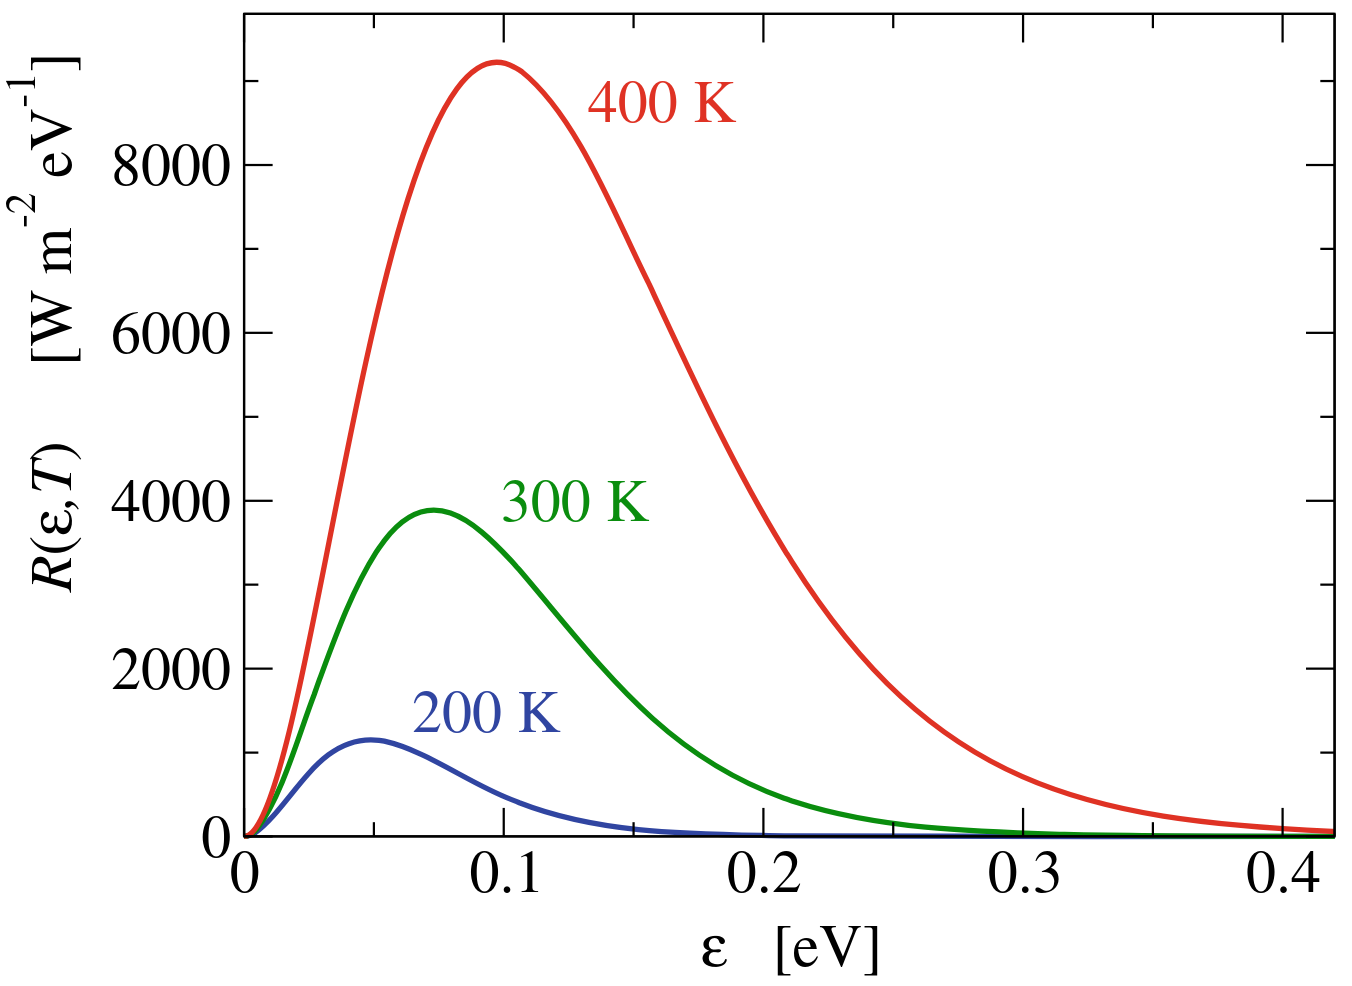
\includegraphics[width = 0.44 \textwidth]{spec-rad.png}
	\caption{Spectral irradiance $ R(E,T) $ of a black body at various temperatures.}
	\label{spec-rad}
\end{figure}

Si può dare consistenza al corpo nero considerando la presenza di radiazione riflessa da parte della sua superficie. Si introduce quindi un coefficiente d'assorbimento $ \alpha(\nu) \in [0,1] $, tale per cui:
\begin{equation}
	R_\text{ass}(\nu,T) = \alpha(\nu) R(\nu,T)
	\qquad \qquad
	R_\text{rif}(\nu,T) = (1 - \alpha(\nu)) R(\nu,T)
\end{equation}
dove $ R(\nu,T) $ è la radianza spettrale incidente. Il corpo nero ha $ \alpha(\nu) \equiv 1 $.

\begin{proposition}{Radianza spettrale emessa}{}
	La radianza spettrale emessa da un corpo non-nero con coefficiente d'assorbimento $ \alpha(\nu) $ è:
	\begin{equation}
		R_\text{em}(\nu,T) = \alpha(\nu) R(\nu,T)
	\end{equation}

	\tcblower

	\begin{proof}
		Dalla conservazione dell'energia $ R(\nu,T) = R_\text{em}(\nu,t) + R_\text{rif}(\nu,T) $, da cui la tesi.
	\end{proof}
\end{proposition}

Si vede dunque che, in generale, $ R_\text{em}(\nu,T) \le R(\nu,T) $, dove l'uguaglianza vale solo per il corpo nero: detta $ R_0(\nu,T) $ la radianza spettrale di corpo nero, si ha $ R_\text{em}(\nu,T) \le R_0(\nu,T) $, dunque non solo i corpi non-neri riflettono parte della radiazione incidente, ma ne emettono anche meno rispetto al corpo nero di uguale temperatura. \\
Tutte queste considerazioni valgono per un sistema all'equilibrio, in cui l'equilibrio termodinamico tra campo elettromagnetico e corpo viene mantenuto dallo scambio di fotoni. Se il corpo viene posto in una regione in cui il campo elettromagnetico è assente, esso perderà energia emettendo fotoni, raffreddandosi di conseguenza: lo spettro di fotoni emessi sarà $ R(\nu,T) = \alpha(\nu) R_0(\nu,T) $, dunque in condizioni di non-equilibrio il corpo nero è quello che si raffredda più velocemente (per irraggiamento); al contrario, il corpo bianco ($ \alpha(\nu) \equiv 0 $) non si raffredderà affatto, in quanto un corpo ideale completamente riflettente non emetterà alcuna radiazione.

\subsection{Interazione radiazione-materia}

Si consideri un ensemble di particelle identiche non-interagenti e, nello spettro single-particle, si considerino soltanto due stati $ \ket{1} , \ket{2} : E_1 < E_2 $. Fotoni risonanti con $ E \approx E_2 - E_1 $ inducono delle transizioni tra questi livelli (si ignorano le transizioni non-risonanti, che avvengono a rate estremamente più bassi). In particolare, la presenza di radiazione induce l'eccitazione $ \ket{1} \rightarrow \ket{2} $ (assorbimento), dunque, definendo la densità d'energia spettrale $ \rho(E) $ (energia per unità di volume ed intervallo spettrale, u.d.m. $ \text{m}^{-3} $), si ha un rate di transizione (u.d.m. $ \text{s}^{-1} $):
\begin{equation}
	R_{1 \rightarrow 2} = B_{12} \rho(E)
\end{equation}
dove $ B_{12} $ è un'opportuna costante dipendente dalle caratteristiche elettro-meccaniche del sistema (si ignorano gli effetti non lineari $ \sim o(\rho^2) $). Per quanto riguarda invece il decadimento $ \ket{2} \rightarrow \ket{1} $ (emissione), esso avviene sia in maniera spontanea che in maniera stimolata, dunque si avrà:
\begin{equation}
	R_{2 \rightarrow 1} = A_{21} + B_{21} \rho(E)
\end{equation}
dove $ B_{21} $ è analoga a $ B_{12} $ ed $ A_{21} $ dà il rate di decadimento spontaneo (in approssimazione di dipolo-elettrico $ A_{21} $ è dato dall'Eq. \ref{eq:electron-trans-prob}). Si noti che, quando un fotone induce un decadimento, il fotone emesso avrà la stessa fase e gli stessi numeri quantici di quello incidente. \\
Queste relazioni valgono indipendentemente dalla condizione del sistema, in quanto i coefficienti dipendono solo dalle sue proprietà microscopiche. In particolare, esse sono valide quando l'ensemble è all'equilibrio rispetto al campo elettromagnetico, nel qual caso $ \rho(E) \equiv u(E,T) $ (funzione di Planck); inoltre, in tale condizione, il numero medio delle particelle nei due stati è uguale, dunque:
\begin{equation}
	[n_1] R_{1 \rightarrow 2} = [n_2] R_{2 \rightarrow 1}
\end{equation}
Inserendo le relative espressioni e risolvendo per $ \rho(E) \equiv u(E,T) $ si trova:
\begin{equation*}
	\frac{\frac{A_{21}}{B_{21}}}{\frac{[n_1]}{[n_2]} \frac{B_{12}}{B_{21}} - 1} = u(E,T) = \frac{1}{\pi^2 c^3 \hbar^3} \frac{E^3}{e^{\beta E} - 1}
\end{equation*}
Dato che all'equilibrio vale la distribuzione di Boltzmann, ovvero $ [n_1] / [n_2] = P_1 / P_2 = e^{\beta (E_2 - E_1)} = e^{\beta E} $, si ottengono così le \textit{relazioni di Einstein}:
\begin{equation}
	B_{12} = B_{21}
	\qquad \qquad
	A_{21} = \frac{E^3}{\pi^2 c^3 \hbar^3} B_{21}
\end{equation}
Ciò conferma le Eqq. \ref{eq:electron-trans-prob}-\ref{eq:stimul-trans-prob}: la prima relazione mostra che il rate stimolato $ \ket{1} \rightarrow \ket{2} $ è uguale a quello $ \ket{2} \rightarrow \ket{1} $, mentre la seconda mostra che, rispetto a quello stimolato, il rate spontaneo ha una dipendenza $ \propto E^3 $.

\subsubsection{Laser}

Le onde elettromagnetiche vengono attenuate quando attraversano un mezzo diverso dal vuoto. Un dispositivo ottico in grado di amplificare la radiazione incidente, piuttosto che ridurla, dovrebbe avere un rate d'emissione superiore a quello d'assorbimento, ovvero:
\begin{equation*}
	\frac{[n_2] R_{2 \rightarrow 1}}{[n_1] R_{1 \rightarrow 2}} = \frac{[n_2]}{[n_1]} \left[ 1 + \frac{A_{21}}{B_{21} \rho(E)} \right] > 1
\end{equation*}
Per un campo elettromagnetico sufficientemente intenso questo rapporto diventa $ [n_2] / [n_1] > 1 $ (infatti $ R_{1 \rightarrow 2} \approx R_{2 \rightarrow 1} $ per campi abbastanza intensi), ovvero un'inversione di popolazione rispetto all'equilibrio $ [n_2] / [n_1] < 1 $. \\
Con un sistema a due livelli non si può avere un laser, in quanto $ 1 < [n_2] / [n_1] = e^{-\beta E} $ implicherebbe $ T < 0 $. Considerando invece un sistema a tre livelli (Fig. \ref{laser}), si devono prendere $ \ket{1},\ket{2},\ket{3} $ tali per cui la transizione $ \ket{1} \rightarrow \ket{3} $, stimolata dal pompaggio ottico, deve essere favorita (elemento di matrice significativamente diverso da 0), $ \ket{3} \rightarrow \ket{2} $ deve essere spontaneamente molto probabile e $ \ket{2} \rightarrow \ket{1} $ deve essere possibile ma poco probabile (ovvero $ \ket{2} $ deve essere uno stato metastabile). In un sistema siffatto è possibile ottenere l'inversione di popolazione $ [n_2] / [n_1] > 1 $. \\
La condizione di metastabilità, che permette di trascurare il decadimento spontaneo $ \ket{2} \rightarrow \ket{1} $, è tanto più difficile da ottenere quanto più è grande $ \Delta E = E_2 - E_1 $, data la dipendenza $ \gamma_{2 \rightarrow 1} \propto \Delta E^3 $: per questo motivo, sono stati prima creati i MASER (Microwave Amplification by Stimulated Emission of Radiation), e solo successivamente i LASER (Light Amplification by Stimulated Emission of Radiation). Si ricordi, infatti, che l'emissione spontanea è per sua natura incoerente, dunque in un laser è necessario avere una dominanza dell'emissione stimolata, che invece è coerente e direzionale\footnote{Dall'equivalenza tra fotoni e oscillatori armonici deriva che l'ampiezza di probabilità per la creazione di un nuovo fotone dipende dall'elemento di matrice dell'operatore di creazione $ \braket{N + 1 | a\dg | N} = \sqrt{N + 1} $ che aumenta all'aumentare di $ N $: nel limite del numero di Avogadro, tale ampiezza tende a $ 1 $, ovvero vengono creati fotoni identici.}.

\begin{figure}
	\centering
	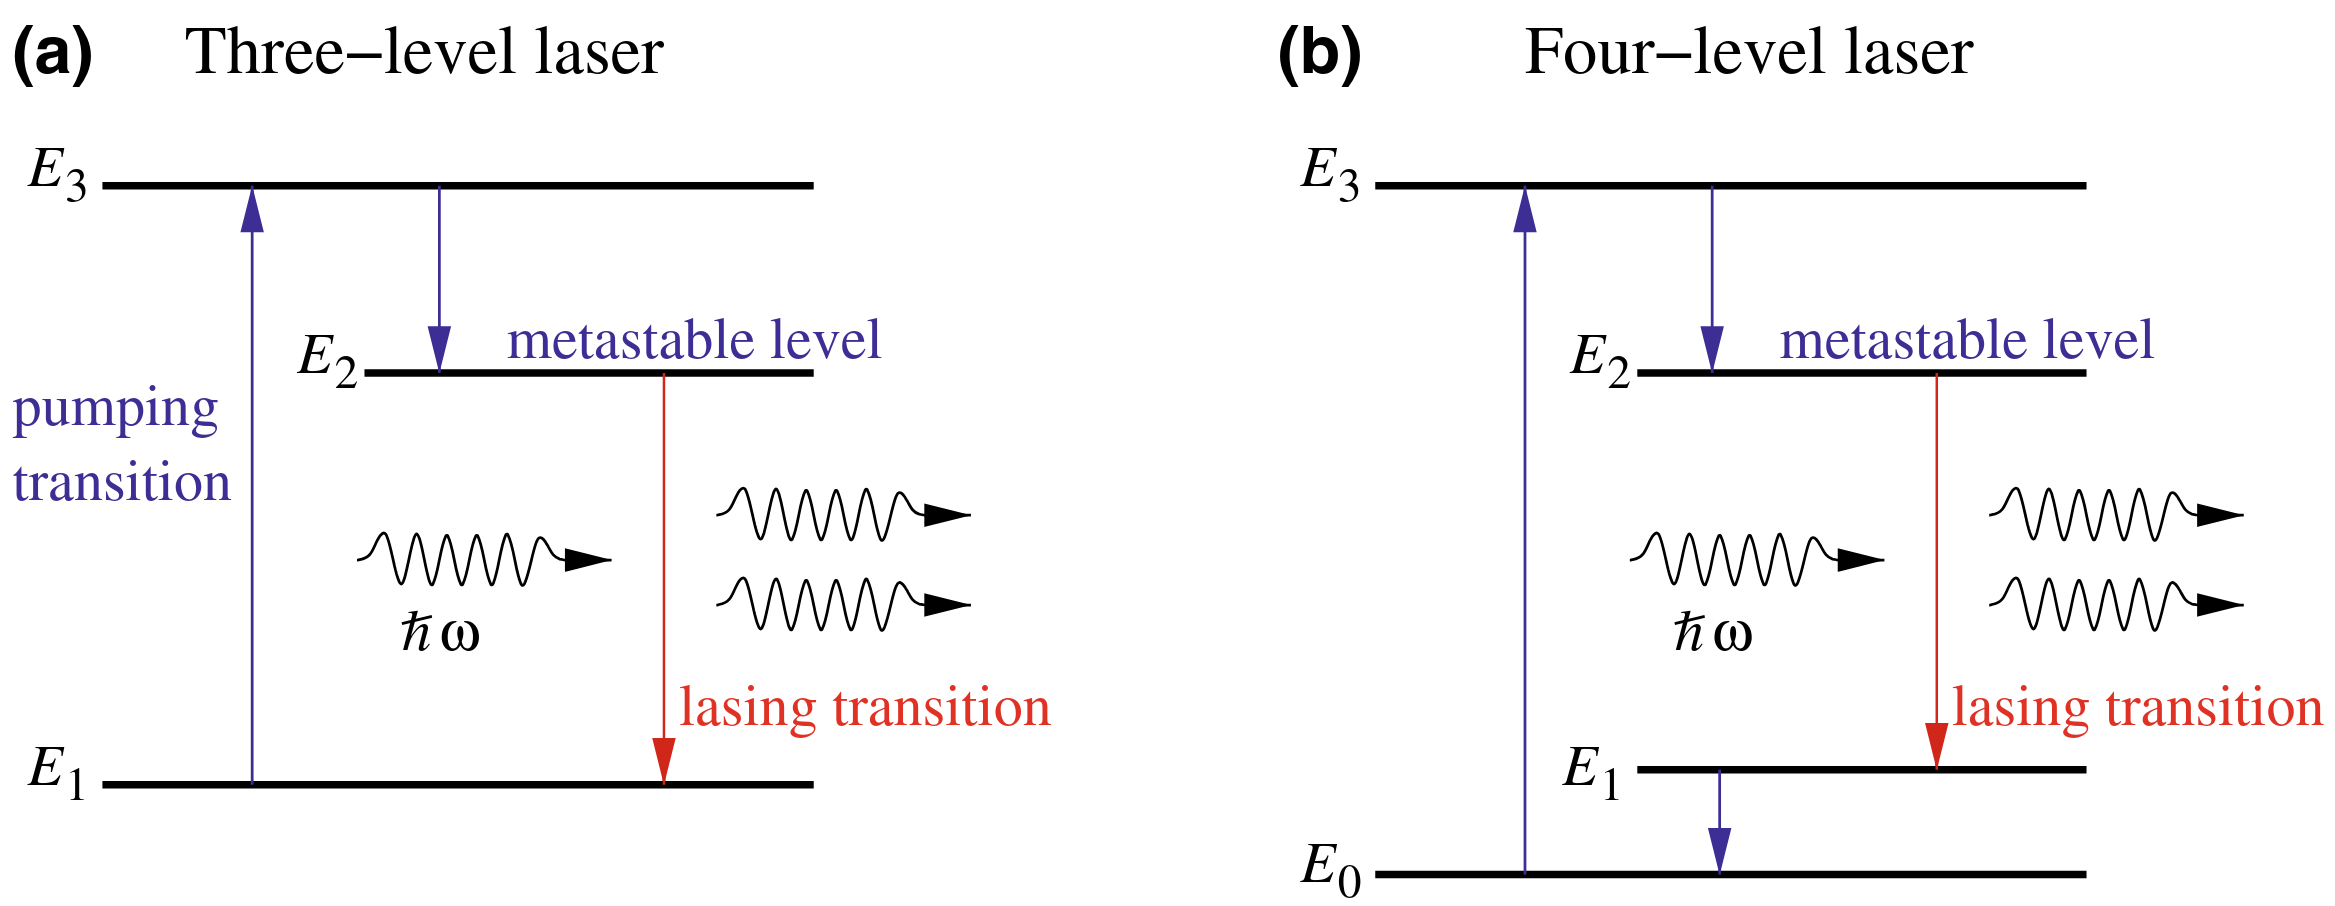
\includegraphics[width = 0.70 \textwidth]{laser.png}
	\caption{Example schemes of lasers.}
	\label{laser}
\end{figure}












\chapter{Solidi Cristallini}
\selectlanguage{italian}

I sistemi macroscopici realizzano l'equilibrio termodinamico bilanciando la tendenza dell'energia interna a diminuire e quella dell'entropia ad aumentare: ad alte temperature prevale il contributo entropico, a basse temperature prevale quello energetico (nei solidi gli atomi hanno posizioni fisse, dunque l'entropia è più basse rispetto ai fluidi). Sperimentalmente, infatti, si trova che quasi tutti i materiali solidificano a temperature abbastanza basse: l'unica eccezione è l'elio, che rimane fluido fino a $ T \approx 0 \,\text{K} $, a meno che non si applichi una sufficiente pressione. \\
Così come la tendenza degli atomi a formare molecole (minimizzando $ V_\text{ad} $) viene misurata dalla binding energy molecolare, la tendenza di atomi/molecole a formare solidi viene misurata da una quantità analoga, l'\textit{energia di coesione}.

\section{Struttura microscopica}

Nello studio di solidi semplici, come ad esempio quelli formati da gas nobili, l'interazione tra atomi è semplificabile a coppie, quindi modellizzabile con il potenziale di Lennard-Jones:
\begin{equation}
	V_\text{ad}(\ve{R}_1 , \dots , \ve{R}_{N_n}) = \sum_{\alpha < \alpha'}^{N_n} V_2(\abs{\ve{R}_\alpha - \ve{R}_{\alpha'}})
	\qquad \qquad
	V_2(r) = 4\varepsilon \left[ \left( \frac{\sigma}{r} \right)^{12} - \left( \frac{\sigma}{r} \right)^6 \right]
\end{equation}
Per un coppia di atomi, la distanza d'equilibrio è $ R_\text{m} = \sqrt[6]{2} \sigma $ con potenziale minimo $ V_2(R_\text{m}) = -\varepsilon $. Inoltre, si vede che il potenziale decade come $ \sim r^{-6} $, quindi, contando che tipicamente il numero di atomi a distanza $ r $ da un dato atomo scala come $ \sim r^2 $, l'energia d'interazione totale a lunga distanza scala come $ r^{-4} $: si vede che ogni atomo interagisce significativamente soltanto con gli atomi ad esso vicini. \\
Si consideri un reticolo 1D di atomi: aggiungendo un terzo atomo ad una coppia di atomi, esso si posizionerà ad una distanza $ \approx R_\text{m} $ da essi (ignorando l'interazione tra secondi-vicini) ed abbasserà la buca di potenziale adiabatico a $ \approx -2\varepsilon $. Ciò è generalizzabile ad $ N_n $ atomi: essi si troveranno a distanza $ \approx R_\text{m} $ l'uno dall'altro e l'energia di coesione totale sarà $ \approx (N_n - 1) \varepsilon $ (circa $ \varepsilon $ per atomo, per $ N_n $ grande). Se si considera l'interazione con secondi- e terzi-vicini, si trova che la distanza d'equilibrio è leggermente minore rispetto a $ R_\text{m} $ e che l'energia di coesione è leggermente maggiore di $ (N_n - 1) \varepsilon $ (si veda Fig. \ref{lat-2}a). \\
Se invece si considera un reticolo 2D, il terzo atomo si posizionerà al vertice di un triangolo equilatero formato con i primi due. Aggiungendo altri atomi, si viene a formare un \textit{reticolo triangolare} (o esagonale, si veda Fig. \ref{lat-2}), in cui ciascun atomo a 6 primi-vicini, dunque l'energia di coesione sarà approssimativamente $ 3\varepsilon $ per atomo (6 legami condivisi da 2 atomi ciascuno). Si vede dunque che il modello d'interazione a coppie porta al principio di \textit{massima coordinazione}: gli atomi si dispongono in modo da massimizzare il numero di primi-vicini, così da massimizzare l'energia di coesione (minimizzando l'energia potenziale adiabatica). \\
Applicando il principio di massima coordinazione ad un reticolo 3D, si vede che 4 atomi massimizzano la loro coordinazione ponendosi ai vertici di un tetraedro regolare: gli atomi successivi si dispongono a formare o il \textit{face-centered cubic lattice} (reticolo fcc, Fig. \ref{lat-3}b) o l'\textit{hexagonal close-packed lattice} (reticolo hcp, Fig. \ref{lat-3}c). In entrambi questi reticoli ogni atomo ha 12 primi-vicini, dunque l'energia reticolare è $ 6\varepsilon $ per atomo; si vede, però, che entrambi sono formati da reticoli triangolari 2D sovrapposti: mentre nell'fcc si ripetono 3 orientazioni diverse, nell'hcp ce ne sono solo 2, dunque, quando si va a considerare l'interazione con secondi- e terzi-vicini, il reticolo fcc è leggermente favorito energeticamente rispetto all'hcp. \\
Confrontando i vari reticoli, si trovano delle distanze d'equilibrio leggermente diverse: in 1D $ R_\text{m} = \sqrt[6]{2} \sigma \simeq 1.22 \sigma $, in 2D $ R_\text{m} \simeq 1.11 \sigma $ ed in 3D $ R_\text{m} \simeq 1.09 \sigma $. Nella tavola periodica c'è una prevalenza a formare cristalli fcc ed hcp: ci sono alcuni bcc (body-centered cubic, simile all'fcc ma con un atomo al centro del cubo, al posto di quelli sulle facce) ed i casi del diamante (struttura a sé) e del polonio, che invece forma l'sc (simple cube). \\
È possibile formare strutture cristalline\footnote{Si noti che i vetri, al contrario dei cristalli, hanno una risposta plastica alle deformazioni: essi non sono solidi, ma liquidi con coefficiente di viscosità estremamente elevato, caratterizzati da livelli energetici estremamente vicini. Infatti, osservando i vedtri di edifici antichi, essi risulteranno ondulati, in quanto deformati nel tempo dalla gravità.} diverse da quelle descritte considerando un potenziale non necessariamente a 2 corpi (valido principalmente per gas nobili, che hanno interazioni deboli): potenziali a più corpi introducono effetti elettronici (quantistici) che danno direzionalità ai legami, fino ad arrivare ai solidi con legami metallici covalenti in cui le interazioni si estendono alla totalità del solido, impedendo di fattorizzare la funzione d'onda.

\begin{figure}[!h]
	\centering
	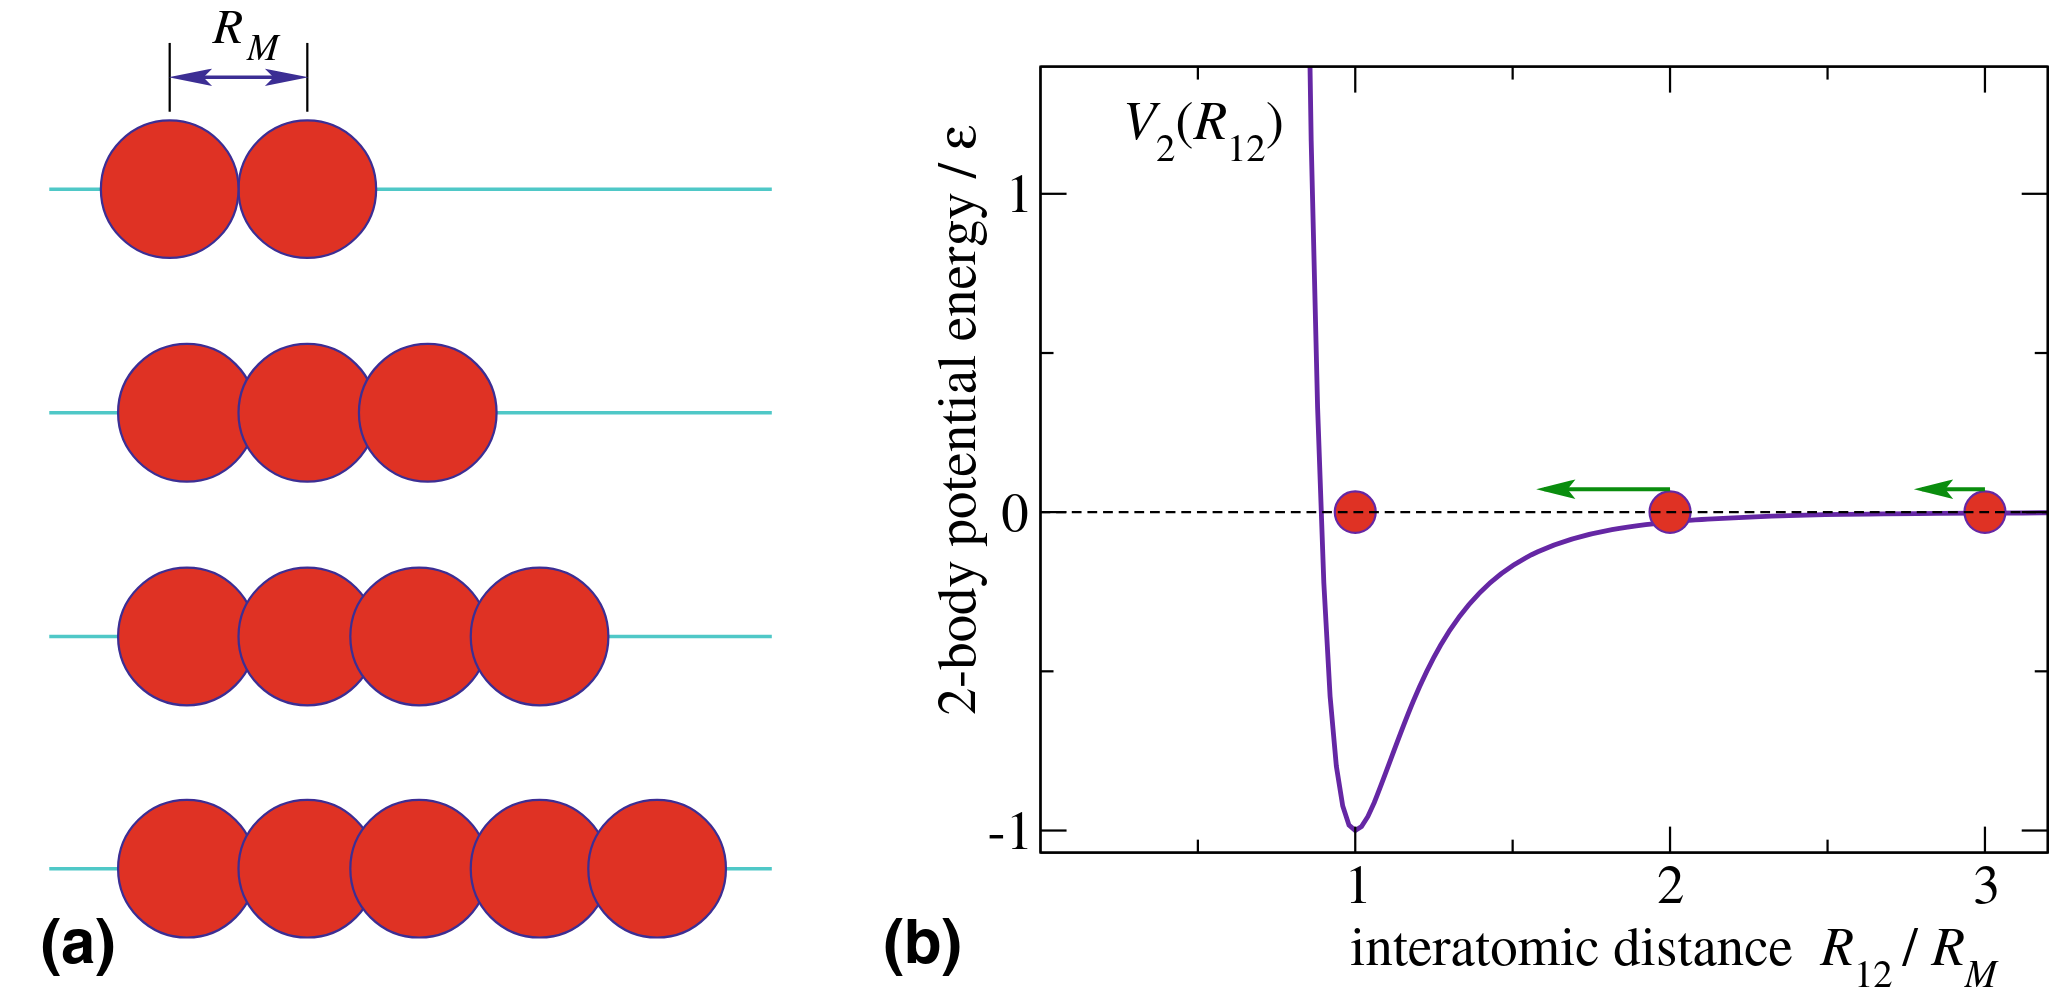
\includegraphics[width = 0.45 \textwidth]{lattice-1d.png}
	\qquad
	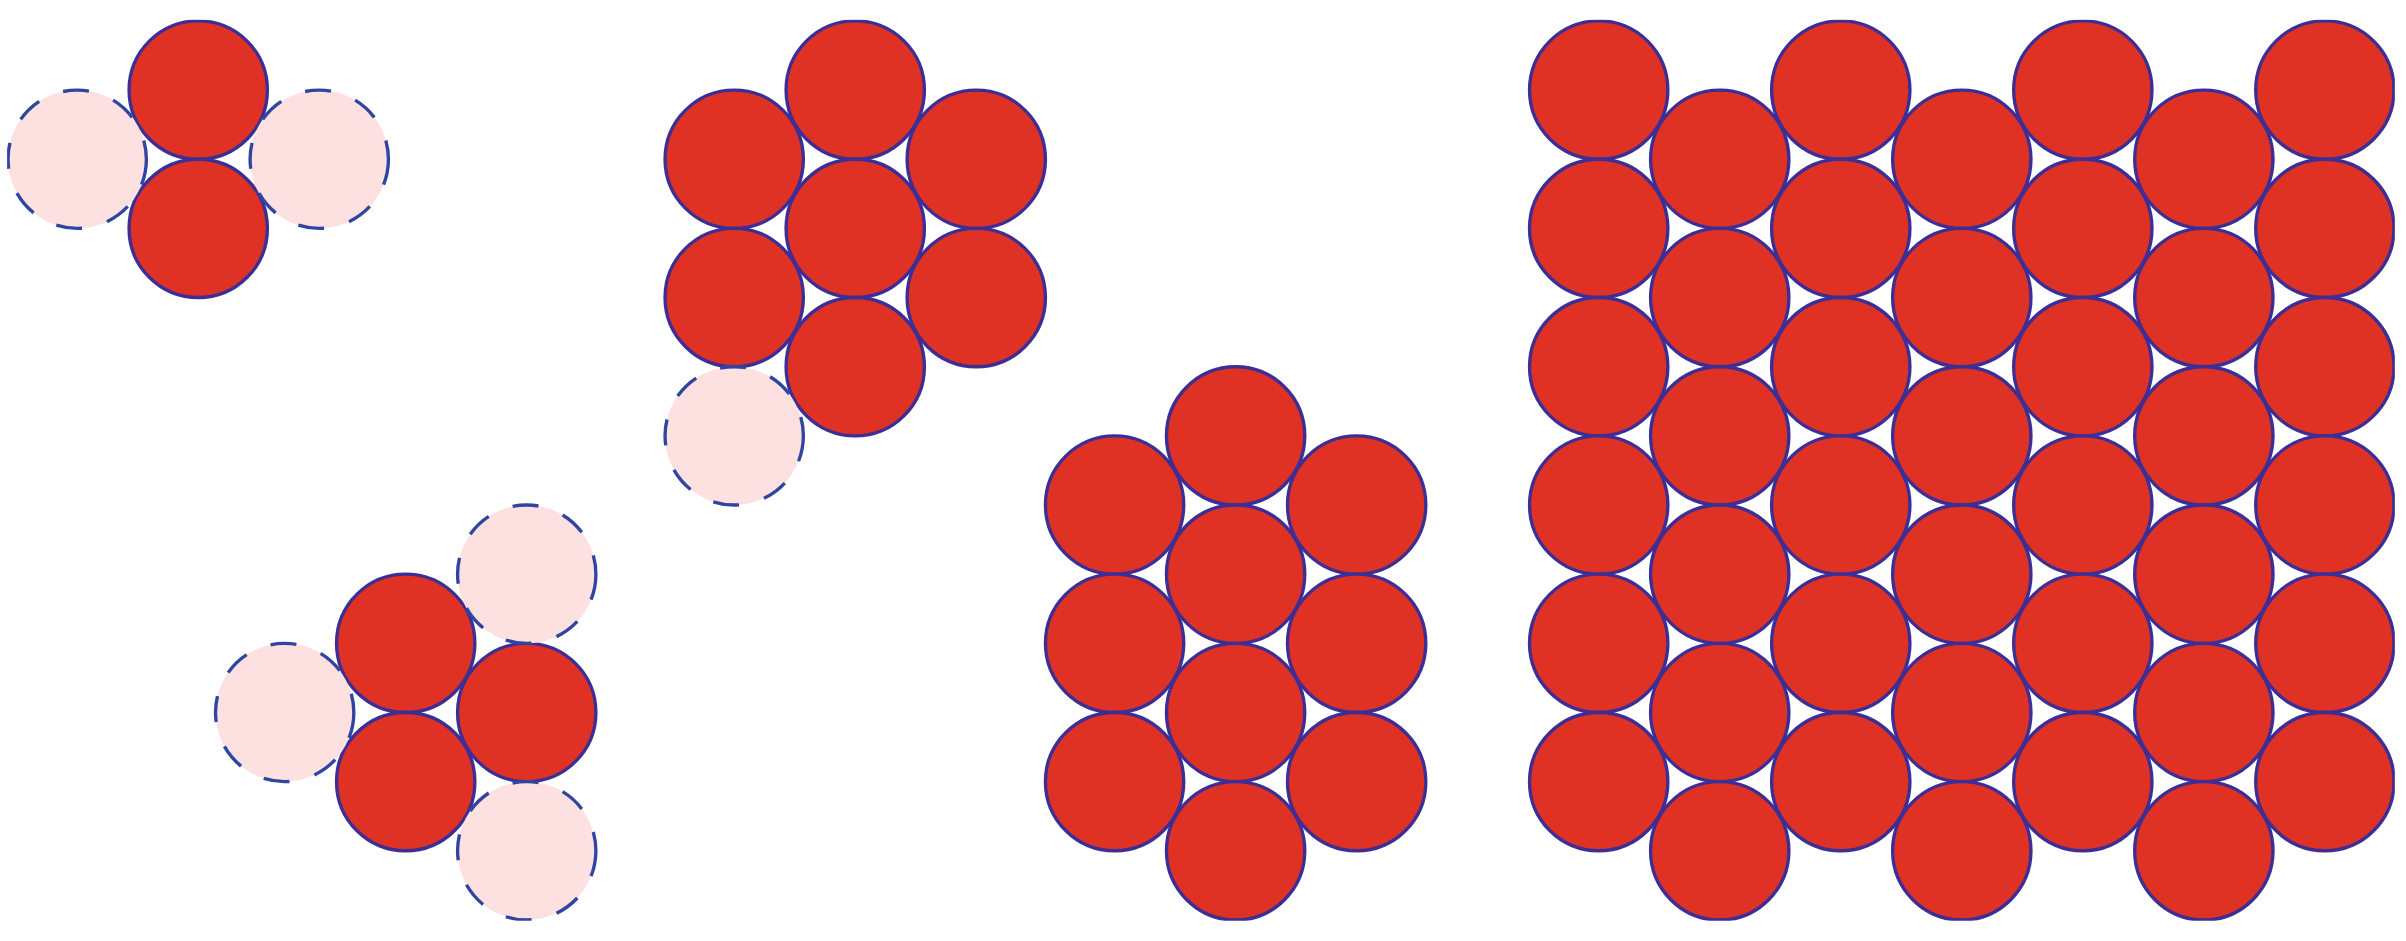
\includegraphics[width = 0.45 \textwidth]{lattice-2d.png}
	\caption{1D lattice and 2D triangular lattice of atoms.}
	\label{lat-2}
\end{figure}
\begin{figure}[!h]
	\centering
	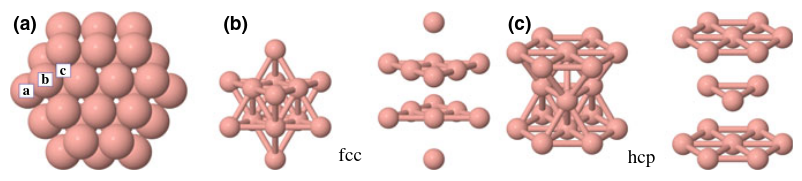
\includegraphics[width = 0.70 \textwidth]{lattice-3d.png}
	\caption{3D lattices of atoms: (a) close packing of spheres, (b) fcc lattice, (c) hcp lattice.}
	\label{lat-3}
\end{figure}

\paragraph{Difetti}

Un cristallo, a qualunque temperatura finita, ha probabilità non-nulla di formare dei \textit{difetti}, come ad esempio un atomo mancante, un atomo aggiuntivo o un'impurità (atomo di tipo diverso). In particolare, essendo il numero di atomi in un cristallo estremamente grande, la concentrazione dei difetti in un cristallo all'equilibrio a bassa temperatura va come $ \sim e^{- \beta E} $ (statistica di Boltzmann), dove $ E \sim 1 \ev $ è l'energia tipica di formazione di un difetto. Termodinamicamente, è impossibile creare un cristallo con un'estensione finita privo di difetti. \\
La piccola differenza energetica tra reticoli fcc ed hcp permette la formazione di difetti estesi (al limite anche macroscopici) come dislocazioni, stacking faults e bordi di grano (vedere Figg. \ref{def-disl}-\ref{def-st-gr}). Una dislocazione avvience quando un layer a cui manca un atomo si collega ad un layer completo: queste configurazioni sono metastabili, e con un'energia finita, a temperatura sufficientemente elevata, è possibile spostare questi difetti all'interno del cristallo. Una stacking fault avviene invece quando si interrompe e viene modificata l'alternanza regolare dei layer, mentre un bordo di grano si verifica quando si sviluppa un cristallo a partire da due punti di duplicazione diversi e con orientazioni diverse, andando a creare un'interfaccia disordinata quando queste orientazioni si incontrano.

\begin{figure}[!h]
	\centering
	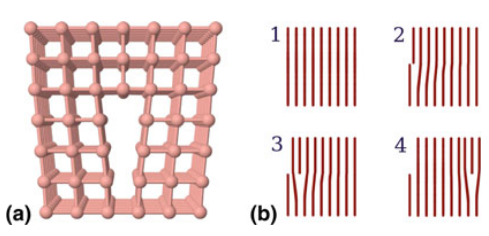
\includegraphics[width = 0.50 \textwidth]{def-disl.png}
	\caption{Dislocation in an sc lattice.}
	\label{def-disl}
\end{figure}
\begin{figure}[!h]
	\centering
	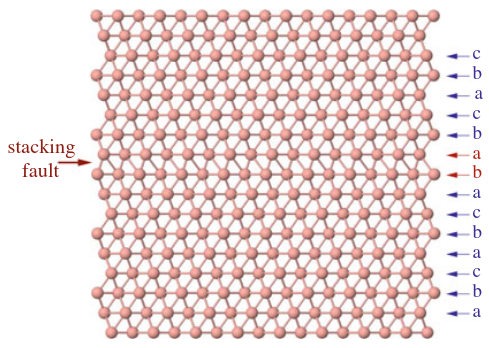
\includegraphics[width = 0.40 \textwidth]{def-st.png}
	\qquad \qquad
	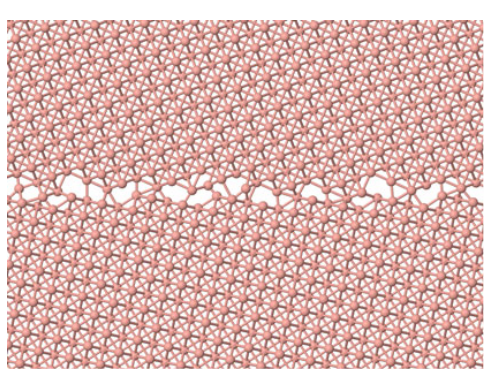
\includegraphics[width = 0.40 \textwidth]{def-gr.png}
	\caption{Stacking fault and grain boundary in an fcc lattice.}
	\label{def-st-gr}
\end{figure}

\subsection{Reticoli cristallini}

Una delle proprietà fondamentali di un solido cristallino è l'equivalenza di varie sue regioni di spazio: infatti, si può assumere che la maggior parte degli atomi di un cristallo si trovino sufficientemente lontani dal suo bordo e da qualsiasi difetto per essere modellato come appartenente ad un cristallo perfetto ed infinitamente esteso. \\
Un cristallo perfetto infinito è un insieme di punti che gode di simmetria traslazionale discreta.

\begin{definition}{Reticolo di Bravais}{}
	Si dice \textit{reticolo di Bravais} $ n $-dimensionale un insieme di punti in $ \R^n $ che risulta invariante per traslazioni discrete:
	\begin{equation}
		\ve{r} \mapsto \ve{r}' = \ve{r} + \ve{R}
		\ , \
		\ve{R} = k_1 \ve{a}_1 + \dots k_n \ve{a}_n
	\end{equation}
	con $ \{k_j\}_{j = 1,\dots,n} \subset \Z $ e $ \{\ve{a}_j\}_{j = 1,\dots,n} \subset \R^n $ linearmente indipendenti.
\end{definition}

I generatori $ \{\ve{a}_j\}_{j = 1,\dots,n} $ vengono detti \textit{primitivi} se sono $ \virgolette{i più piccoli possibili} $ (non univocamente definiti) e formano una cella primitiva, ovverosia il volume minimo che contiene tutti i punti traslazionalmente non-equivalenti del reticolo (a meno di traslazioni) e che, ripetuto nello spazio tramite traslazioni discrete, riproduce il reticolo. Nel caso tridimensionale, il volume della cella primitiva è $ V_c = \abs{(\ve{a}_1 \cdot \ve{a}_2) \times \ve{a}_3} $. \\
La cella primitiva contiene tutta l'informazione del reticolo (che è una ripetizione di tale cella), dunque il suo studio è fondamentale. Il problema, nel definirla, è che non c'è un univoco set di vettori primitivi.

\begin{definition}{Cella di Wigner-Seitz}{}
	Dato punto $ \ve{R} $ in un reticolo di Bravais, si definisce la \textit{cella di Wigner-Seitz} l'insieme di punti $ \ve{r} $ più vicini ad $ \ve{R} $ rispetto ad un altro punto $ \ve{R}' $ del reticolo.
\end{definition}

\begin{proposition}{}
	La cella di Wigner-Seitz è una cella primitiva.
\end{proposition}

L'introduzione della cella di Wigner-Seitz elimina l'arbitrarietà nella scelta della cella primitiva.

\begin{figure}
	\centering
	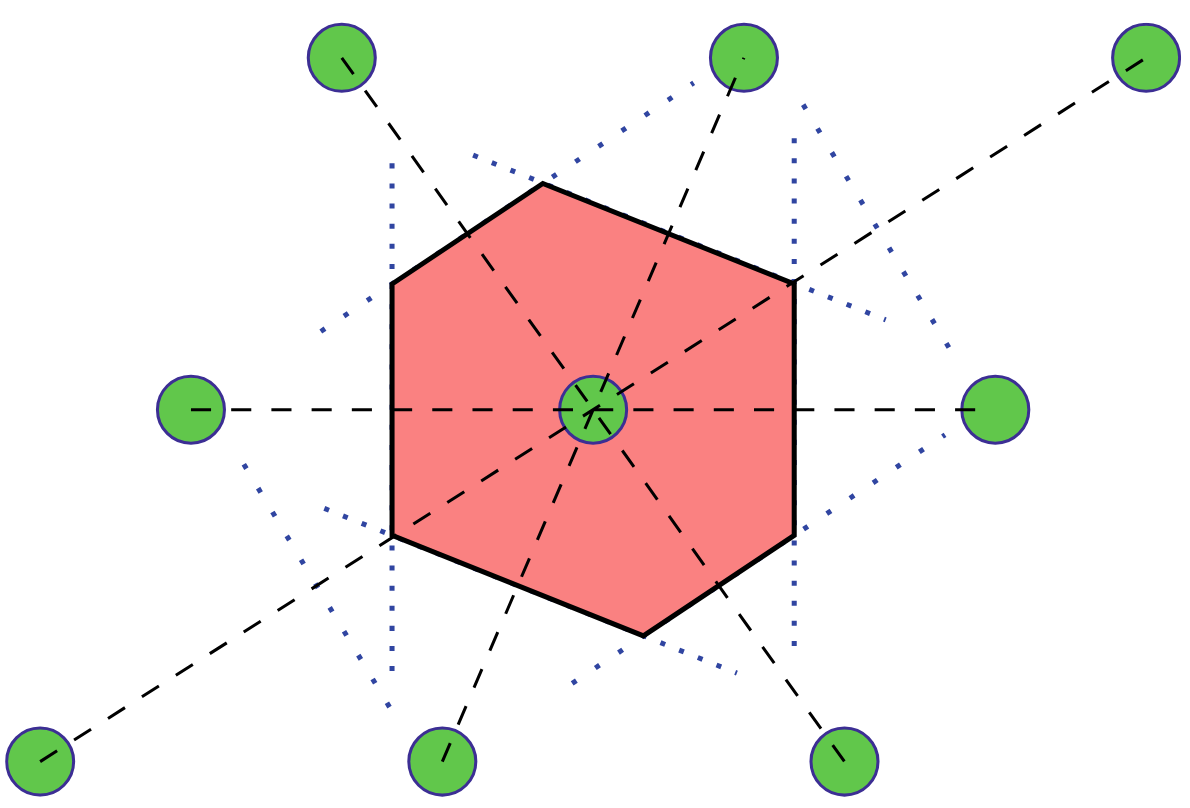
\includegraphics[width = 0.50 \textwidth]{ws-2.png}
	\caption{Wigner-Seitx cell for a 2D lattice.}
	\label{ws-2}
\end{figure}
\begin{figure}
	\centering
	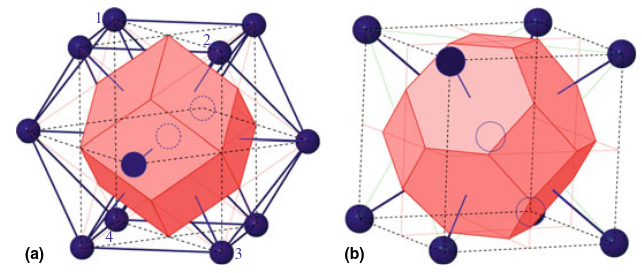
\includegraphics[width = 0.50 \textwidth]{ws-3.png}
	\quad
	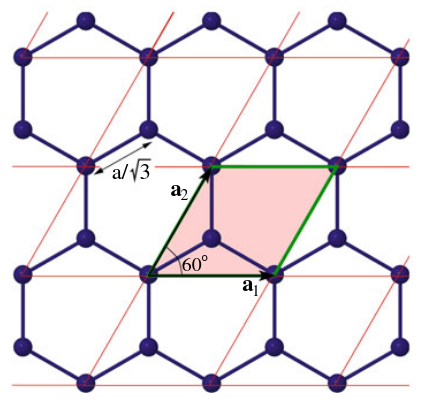
\includegraphics[width = 0.30 \textwidth]{ws-g.png}
	\caption{Wigner-Seitx cell for the fcc lattice, the bcc lattic and graphene.}
	\label{ws-3}
\end{figure}

Si noti che, in generale, una cella primitiva può contenere più di un atomo (es.: $ \ch{Na Cl} $, grafite, etc.). Infatti, un cristallo è definito da un reticolo di Bravais e da una base, ovvero un insieme di uno o più atomi ripetuti in ogni punto del retivolo. È inoltre conveniente trattare le cosiddette \textit{celle convenzionali}, ovvero insiemi di una o più celle primitive che hanno forme preferibilmente cubiche (fcc, bcc o sc), per facilitare la trattazione. Bisogna tener conto che le celle convenzionali, essendo delle super-celle, contengono informazioni ridondanti rispetto alle celle primitive.

\subsubsection{Reticolo reciproco}

Si consideri una funzione $ f : \R \rightarrow \R $ periodica con periodo $ a \in \R $, ovvero tale per cui $ f(x -na) = f(x) \,\,\forall n \in \Z $. La sua antitrasformata di Fourier è:
\begin{equation}
	f(x) = \int_\R \frac{\dd k}{\sqrt{2\pi}} e^{ikx} \tilde{f}(k)
\end{equation}
I coefficienti di Fourier $ \tilde{f}(k) $ sono nulli, eccetto quelli con lo stesso periodo di $ f(x) $, ovvero quelli con $ e^{ikx} = e^{ik(x-a)} $: ciò equivale a $ e^{-ika} = 1 $, ovvero $ k = \ell \frac{2\pi}{a} $, con $ \ell \in \Z $. Questi valori vengono convenzionalmente indicati come:
\begin{equation}
	G = \frac{2\pi}{a} \ell
\end{equation}
e forniscono le frequenze discrete, nello spazio reciproco, che costituiscono la serie di Fourier di $ f(x) $:
\begin{equation}
	f(x) = \sum_G e^{iGx} \tilde{f}(G)
	\qquad \qquad
	\tilde{f}(G) = \frac{1}{a} \int_0^a \dd x\, e^{-i G x} f(x)
\end{equation}
I punti $ G $ nello spazio reciproco formano un reticolo, detto \textit{reticolo reciproco}, legato al reticolo nello spazio diretto da:
\begin{equation}
	e^{i G R} = e^{i 2\pi n \ell} = 1
\end{equation}
dove $ R = na $ sono le traslazioni del reticolo diretto. Si trova quindi $ \ell = \frac{1}{n} $. \\
Queste definizioni sono generalizzabili al caso 3D, in cui $ \ve{R} = n_1 \ve{a}_1 + n_2 \ve{a}_2 + n_3 \ve{a}_3 $. In questo caso, la condizione di reciprocità diventa:
\begin{equation}
	e^{i \ve{G} \cdot \ve{R}} = 1
	\label{eq:rec-ret}
\end{equation}
In 3D si trova che:
\begin{equation}
	\ve{G} = \ell_1 \ve{b}_1 + \ell_2 \ve{b}_2 + \ell_3 \ve{b}_3
\end{equation}
con $ \ell_1, \ell_2, \ell_3 \in \Z $ e:
\begin{equation}
	\ve{b}_1 = \frac{2\pi}{V_c} \ve{a}_2 \times \ve{a}_3
	\qquad
	\ve{b}_1 = \frac{2\pi}{V_c} \ve{a}_2 \times \ve{a}_3
	\qquad
	\ve{b}_1 = \frac{2\pi}{V_c} \ve{a}_2 \times \ve{a}_3
\end{equation}
Si noti che $ \ve{a}_i \cdot \ve{b}_j = 2\pi $, dunque $ \ve{G} \cdot \ve{R} = 2\pi (n_1 \ell_1 + n_2 \ell_2 + n_3 \ell_3) $. La serie di Fourier in 3D diventa:
\begin{equation}
	f(\ve{x}) = \sum_\ve{G} e^{i \ve{G} \cdot \ve{x}} \tilde{f}(\ve{G})
	\qquad \qquad
	\tilde{f}(\ve{G}) = \frac{1}{V_c} \int_{V_c} \dd^3x\, e^{-i \ve{G} \cdot \ve{x}} f(\ve{x})
\end{equation}
Il volume della cella primitiva del reticolo reciproco è $ \tilde{V}_c = (\ve{b}_1 \times \ve{b}_2) \cdot \ve{b}_3 = \frac{(2\pi)^3}{V_c} $: questa viene detta \textit{prima zona di Brillouin} (BZ).

\begin{example}{Reticoli reciproci}{}
	Il reticolo reciproco di un fcc con cubo di lato $ a $ è un bcc con cubo di lato $ 4\pi/a $ e viceversa, mentre il reticolo reciproco di un sc con cubo di lato $ a $ è un sc con cubo di lato $ 2\pi/a $.
\end{example}

Ciascun $ \ve{G} $ nel reticolo reciproco definisce un'onda piana $ e^{i \ve{G} \cdot \ve{x}} $ (nello spazio diretto) con la stessa periodicità del reticolo diretto. Se si considerano i fronti d'onda fissati, per esempio, da $ e^{i \ve{G} \cdot \ve{x}} = 1 $, questi formano una famiglia di piani paralleli tra loro e perpendicolari a $ \ve{G} $ (che ne dà la direzione di propagazione), separati tra loro da una distanza $ \lambda = 2\pi / \abs{\ve{G}} $. \\
Alcuni di questi piani passano per punti del reticolo reciproco; in particolare, tutti questi piani passano per punti del reticolo reciproco se gli indici interi $ (\ell_1 \, \ell_2 \, \ell_3) $ che definiscono $ \ve{G} $ non hanno divisori non-banali comuni: questi vengono detti \textit{indici di Miller} della famiglia di piani considerata. Se invece $ \ve{G} $ è determinato da $ (n\ell_1 \, n\ell_2 \, n\ell_3) $, con $ n \in \Z - \{0\} $, allora soltanto un piano ogni $ n $ passerà per punti del reticolo diretto. \\
Si dimostra che gli indici di Miller sono proporzionali ai reciproci delle intercette dei piani con le direzioni dei vettori primitivi del reticolo diretto.

\subsection{Diffrazione}

La diffrazione da sonde wave-like è il principale mezzo d'indagine della struttura interna dei cristalli, data la loro natura periodica. La lunghezza d'onda di tali sonde deve essere comparabile con la tipica dimensione delle celle primarie del cristallo, tipicamente $ \sim 0.1 - 1 \,\text{nm} $: ciò corrisponde ad elettroni con energia cinetica $ \sim 1.5 - 150 \ev $, raggi X nel range $ \sim 1 - 10 \kev $ o neutroni con energia cinetica $ \sim 1 - 100 \,\text{meV} $. Gli elettroni interagiscono fortemente con la materia, dunque sono sensibili solo agli strati superficiali del cristallo; se si escludono energie risonanti con stati di core atomici, i raggi X riescono a penetrare anche per migliaia di celle primarie, andando a sondare le proprietà di bulk del cristallo; infine i neutroni, interagendo solo coi nuclei (dunque con sezione d'urto molto piccola), riescono a penetrare anche nell'ordine del centimetro. \\
Si assuma che il raggio incidente sia prodotto da una sorgente lontana, così da avere un vettore d'onda $ \ve{k} $ ben definito (con $ \abs{\ve{k}} = 2\pi/\lambda) $, e che il raggio uscente sia rilevato da un detector lontano, così da rilevare un $ \ve{k}' $ ben definito. Nell'ipotesi di scattering elastico, si ha $ \abs{k} = \abs{k}' $ (ovvero $ \lambda = \lambda' $) e si definisce il vettore d'onda trasferito come $ \ve{q} \equiv \ve{k}' - \ve{k} $. Dato che ogni volume infinitesimo $ \dd^3r $ scattera il raggio incidente in porporzione al numero di scatterers in esso presente $ n(\ve{r}) \dd^3r $ (con $ n(\ve{r}) $ densità numerica), la probabilità totale di osservare lo scattering $ \ve{k} \rightarrow \ve{k}' $ è (ricordando che sono onde):
\begin{equation*}
	P_{\ve{k} \rightarrow \ve{k}'} \propto \abs{\int_V \dd^3r\, n(\ve{r}) e^{-i \ve{k}' \cdot \ve{r}} e^{i \ve{k} \cdot \ve{r}}}^2 = \abs{\int_V \dd^3r\, n(\ve{r}) e^{-i \ve{q} \cdot \ve{r}}}^2 \propto \abs{\tilde{n}(\ve{q})}^2
\end{equation*}
dove $ \tilde{n}(\ve{q}) $ è la trasformata di Fourier della densità numerica di scatterers $ n(\ve{r}) $ (a seconda della sonda, sarà la densità numerica di nuclei $ n_\text{nucl}(\ve{r}) $ se la sonda è composta da neutroni, mentre sarà quella di elettroni $ n_\text{el}(\ve{r}) $ se composta da raggi X). Si trova quindi che l'intensità del fascio scatterato va come:
\begin{equation}
	I(\ve{q}) \propto \abs{\tilde{n}(\ve{q})}^2
\end{equation}
La densità numerica di un solo atomo è una $ \delta $ di Dirac, ed infatti l'intesità da scatter neutronico di un solo atomo è essenzialmente indipendente da $ \ve{q} $, come si vede in Fig. \ref{diffr}. \\
Se invece si considerano due atomi, si avrà inferferenza tra i raggi scatterati dai due centri di diffusione. Considerando le posizioni $ \ve{R}_1 , \ve{R}_2 $ dei due atomi, si ha qualitativamente che:
\begin{equation*}
	\begin{split}
		\abs{\tilde{n}(\ve{q})}^2
		& \propto \abs{e^{-i \ve{R}_1 \cdot \ve{q}} + e^{-i \ve{R}_2 \cdot \ve{q}}}^2 = \abs{\exp \left( -i \frac{\ve{R}_1 + \ve{R}_2}{2} \cdot \ve{q} \right) 2 \cos \left( \frac{\ve{R}_1 - \ve{R}_2}{2} \cdot \ve{q} \right)}^2 \\
		& = 2 \left[ 1 + \cos \left( (\ve{R}_1 - \ve{R}_2) \cdot \ve{q} \right) \right] = 2 \left[ 1 + \cos (a q_x) \right]
	\end{split}
\end{equation*}
dove si è supposto che $ \ve{R}_1 - \ve{R}_2 = a \hat{\ve{e}}_x $ e $ \hat{\ve{e}}_x \cdot \ve{q} = q_x $. Si vede dunque che la condizione di interferenza costruttiva (così da avere picchi di diffrazione) è:
\begin{equation*}
	aq_x = 2\pi \ell
	\qquad \Rightarrow \qquad
	q_x = \frac{2\pi}{a} \ell
\end{equation*}
Considerando un reticolo 3D di $ N $ atomi, quindi, la trasformata della densità numerica va come:
\begin{equation*}
\abs{\tilde{n}(\ve{q})}^2 \propto \abs{\sum_{j = 1}^N e^{-i \ve{R}_j \cdot \ve{q}}}^2
\end{equation*}
La condizione d'interferenza costruttiva è quindi:
\begin{equation}
	e^{-i \ve{R} \cdot \ve{q}} = 1 \quad \forall \ve{R} \in \text{reticolo}
	\label{eq:cond-int-cos}
\end{equation}
Questa non è altro che l'Eq. \ref{eq:rec-ret}: si trova quindi che i picchi di diffrazione, detti \textit{picchi di Bragg}, si hanno per vettori d'onda trasferiti appartenente al reticolo recièroco, ovvero per $ \ve{q} = \ve{G} $. Si noti che può accadere che la condizione \ref{eq:cond-int-cos} può essere verificata anche solo per alcuni $ \ve{R} \in \text{reticolo} $: in tal caso, si hanno dei picchi di diffrazione secondari, la cui intensità decresce rapidamente all'aumentare del numero di atomi nel reticolo (si veda Fig. \ref{diffr}).

\begin{figure}
	\centering
	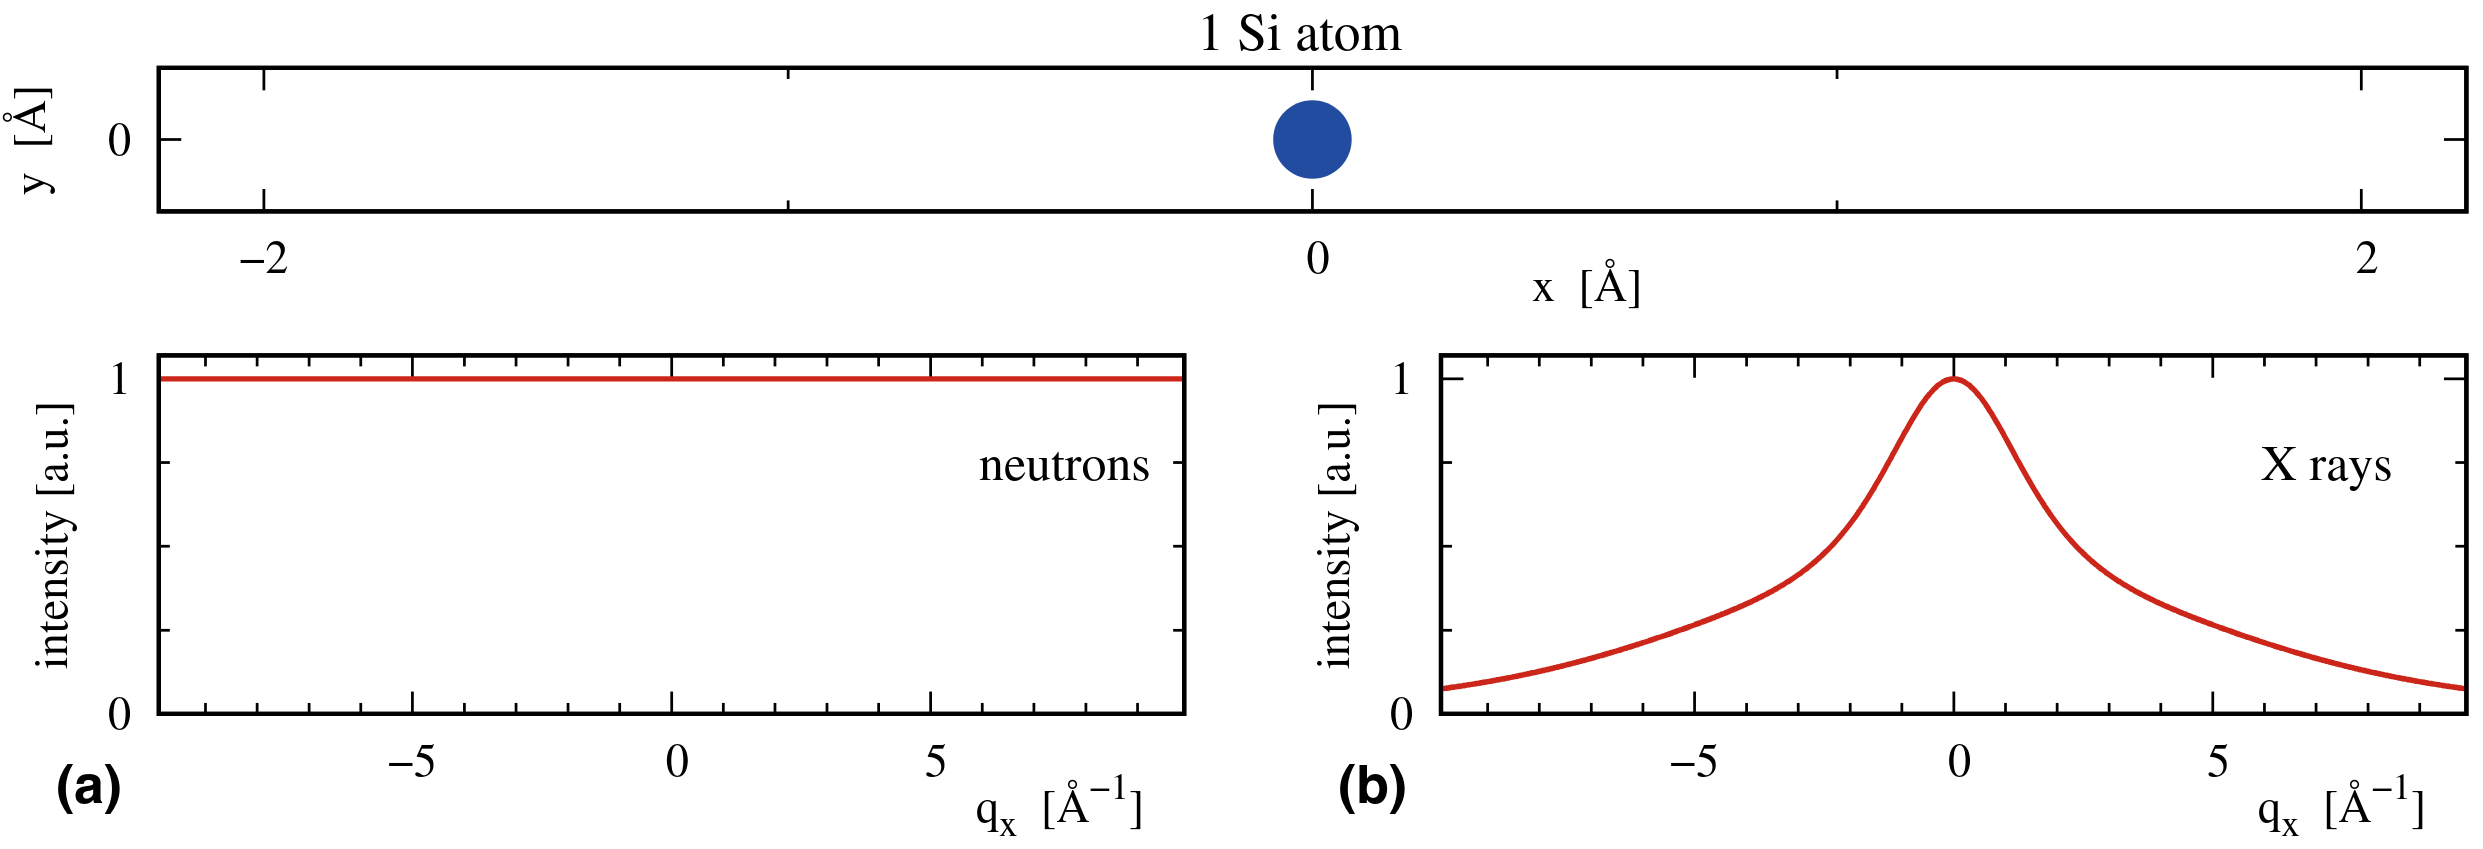
\includegraphics[width = 0.70 \textwidth]{diffr-1.png}
	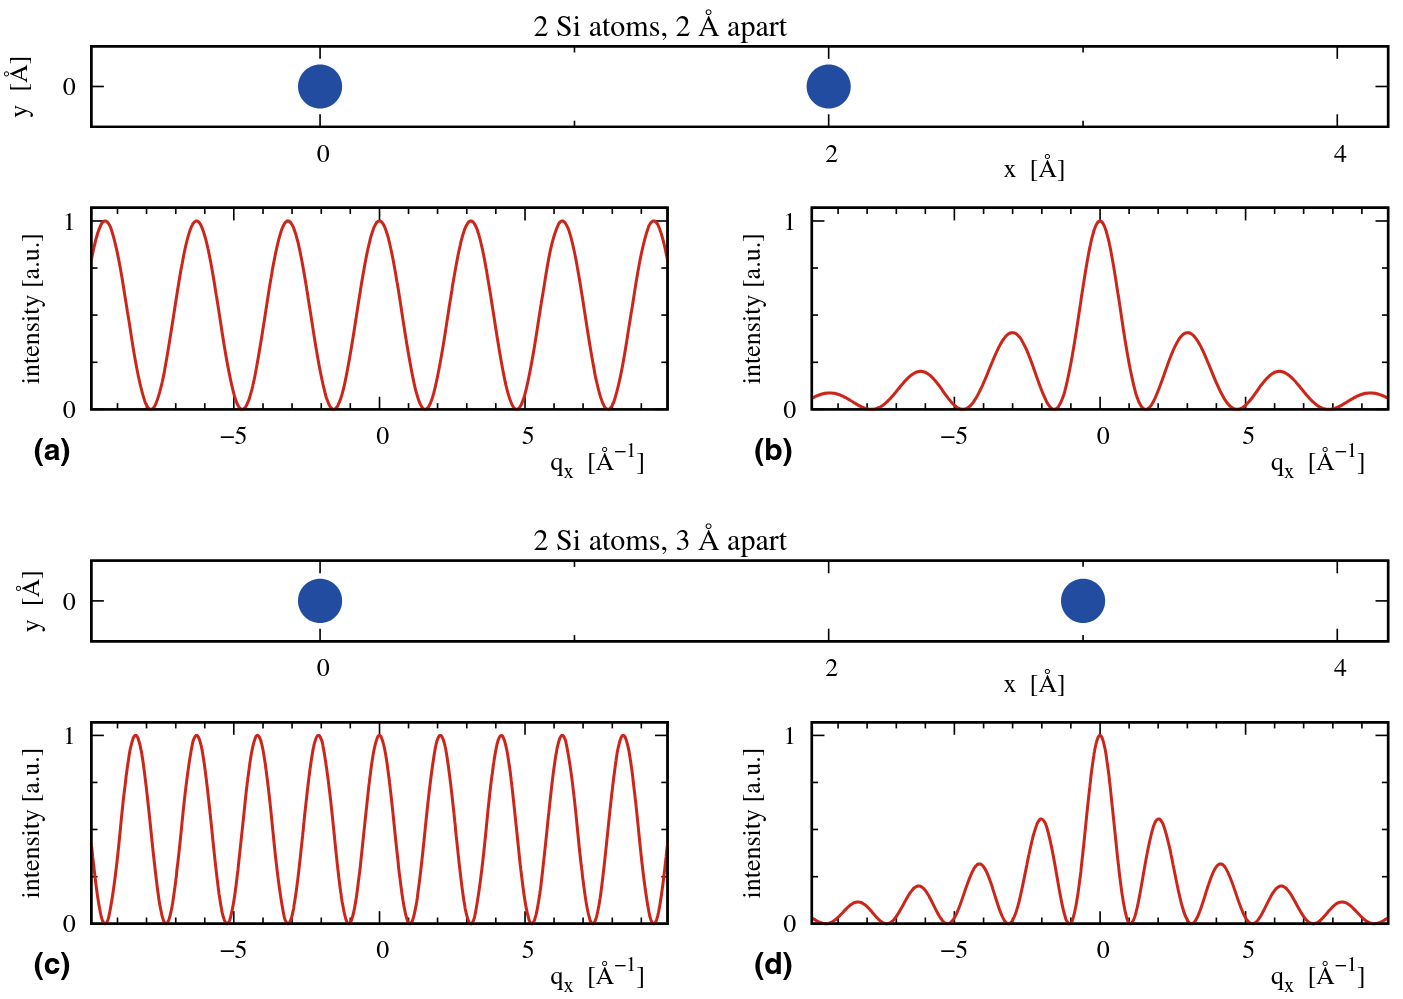
\includegraphics[width = 0.70 \textwidth]{diffr-2.png}
	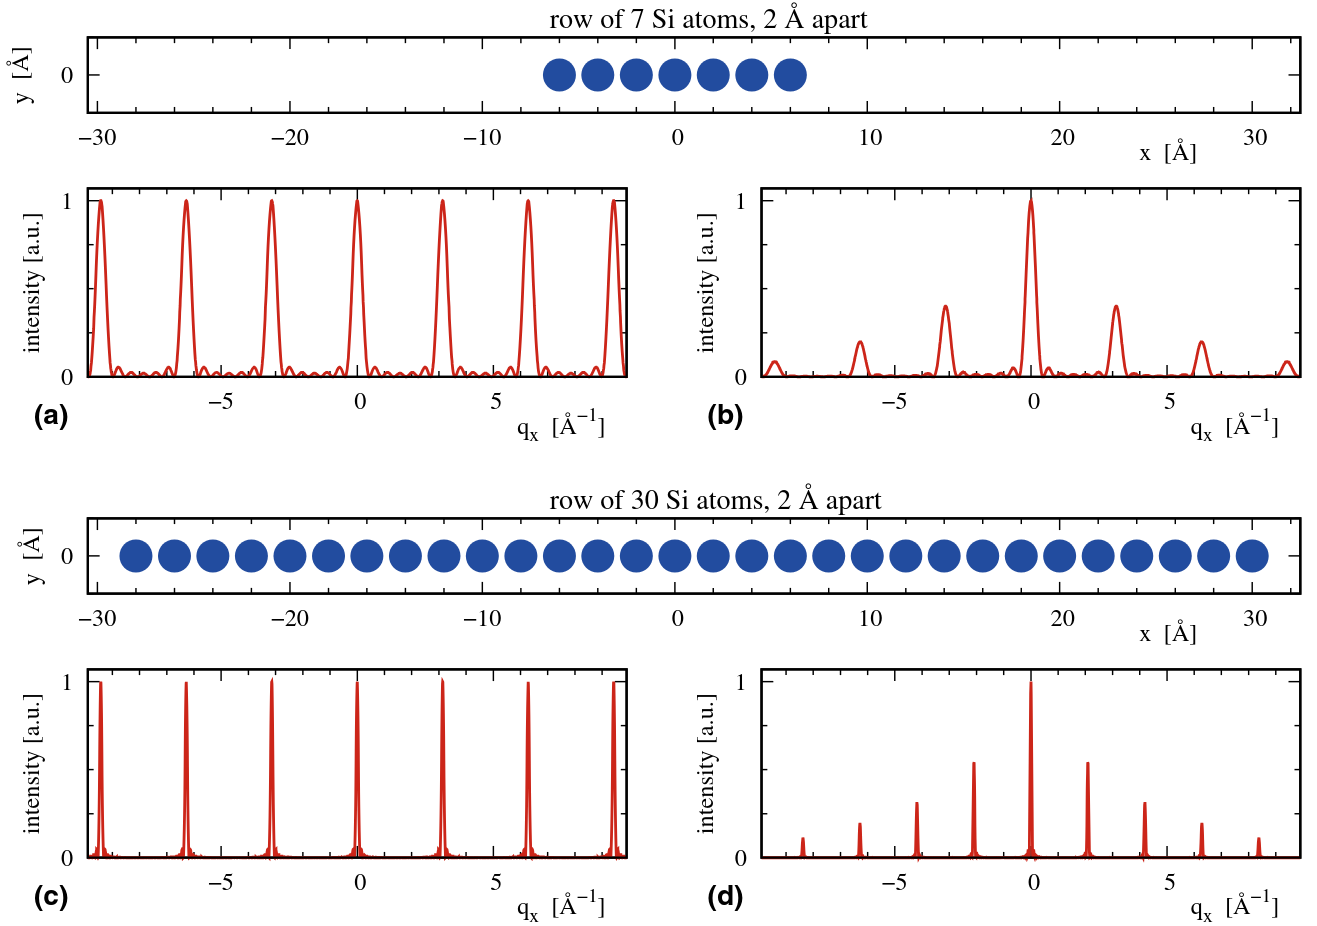
\includegraphics[width = 0.70 \textwidth]{diffr-3.png}
	\caption{Diffraction patterns of various 1D chains of $ \ch{Si} $ atoms.}
	\label{diffr}
\end{figure}

\subsubsection{Fattori di forma}

Raggi X che scatterano su un singolo atomo ne sondano la distribuzione di densità elettronica $ n_\text{at}(\ve{r}) $, tramite il \textit{fattore di forma atomico} $ f_\text{at}(\ve{q}) = \tilde{n}_\text{at}(\ve{q}) $: questo ha una caratteristica forma a campana con $ f_\text{at}(\ve{0}) $ pari al quadrato del numero di elettroni. \\
Per $ Z \gg 1 $, gli elettroni di core scatterano di più i raggi X rispetto ai meno numerosi elettroni di valenza, così che, per un insieme di atomi, la distribuzione elettronica vista dai raggi X possa essere approssimata come la somma delle individuali distribuzioni atomiche:
\begin{equation}
	n_\text{el}(\ve{r}) = \sum_\ve{R} n_\text{at}(\ve{r} - \ve{R})
\end{equation}
La presenza di legami chimici deforma soltanto i relativamente pochi elettroni di valenza, così che tale approssimazione dia un buon accordo sperimentale. Calcolando la trasformata di Fourier:
\begin{equation*}
	\begin{split}
		\tilde{n}_\text{el}(\ve{q})
		& = \sum_\ve{R} \int \dd^3r\, n_\text{at}(\ve{r} - \ve{R}) e^{-i \ve{q} \cdot \ve{r}} = \sum_\ve{R} \int \dd^3r'\, n_\text{at}(\ve{r}') e^{-i \ve{q} \cdot (\ve{r}' + \ve{R})} \\
		& = \sum_\ve{R} e^{-i \ve{q} \cdot \ve{R}} \int \dd^3r\, n_\text{at}(\ve{r}) e^{-i \ve{q} \cdot \ve{r}} \equiv \tilde{n}_\text{ret}(\ve{q}) f_\text{at}(\ve{q})
	\end{split}
\end{equation*}
Si hanno dunque due contributi moltiplicativi (si ricordi che un prodotto nello spazio reciproco è una convoluzione nello spazio reale): $ \tilde{n}_\text{ret}(\ve{q}) $, che descrive lo scattering da oggetti puntiformi posti nei nodi del reticolo di Bravais, ed $ f_\text{at}(\ve{q}) $, che descrive lo scattering dagli atomi singoli. Dato che $ n_\text{nuc}(\ve{r}) \propto n_\text{ret}(\ve{r}) $, si trova una relazione tra l'intensità della diffrazione da raggi X e quella da neutroni:
\begin{equation}
	I_\text{X}(\ve{q}) \propto \abs{f_\text{at}(\ve{q})}^2 \abs{\tilde{n}_\text{nuc}(\ve{q})}^2 \propto \abs{f_\text{at}(\ve{q})}^2 I_\text{n}(\ve{q})
\end{equation}
Questa relazione di proporzionalità è confermata in Fig. \ref{diffr}: i raggi X scatterano nelle stesse direzioni e con le stesse lunghezze d'onda dei neutroni, ma l'intensità dei picchi è modulata da $ \abs{f_\text{at}(\ve{q})}^2 $. \\
Se si considerano cristalli poliatomici la cui cella primitiva contiene $ n_d $ atomi, la derivazione rimane invariata, sommando anche su questi atomi:
\begin{equation}
	n_\text{el}(\ve{r}) = \sum_\ve{R} \sum_{j = 1}^{n_d} n_{\text{at},j}(\ve{r} - \ve{d}_j - \ve{R})
\end{equation}
Si trova così che il fattore di forma atomico va sostituito con un \textit{fattore di struttura}:
\begin{equation}
	S(\ve{q}) = \sum_{j = 1}^{n_d} e^{-i \ve{q} \cdot \ve{d}_j} f_{\text{at},j}(\ve{q})
\end{equation}
rappresentante la trasformata di Fourier della distribuzione elettronica degli $ n_d $ atomi nella cella primaria. Nello scattering di neutroni, gli $ f_{\text{at},j}(\ve{q}) $ sono sostituiti da ampiezze di scattering neutronico indipendenti da $ \ve{q} $. Si trova dunque che, posto $ \abs{f_\text{at}(\ve{q})}^2 \mapsto \abs{S(\ve{q})}^2 $, la forma di $ I(\ve{q}) $ rimane pressoché invariata: ciò significa che il pattern di diffrazione è sostanzialmente indipendente dal numero di atomi nella cella primaria, ma è determinato dal reticolo di Bravais del cristallo; gli atomi nella cella primaria vanno soltanto a modificare moltiplicativamente l'intensità, senza modificarne la forma.

\subsubsection{Scattering di Bragg}

Come si è visto, la condizione per cui si hanno picchi di diffrazione è $ \ve{q} = \ve{G} $. In aggiunta a ciò, per avere scattering elastico è necessario che $ \abs{\ve{k}} = \abs{\ve{k}'} $, ovvero:
\begin{equation}
	\abs{\ve{k}} = \abs{\ve{k} + \ve{G}}
	\label{eq:bragg-diffr}
\end{equation}
Questa condizione corrisponde geometricamente ad una sfera nello spazio reciproco, rappresentata dalla \textit{costruzione di Ewald} (Fig. \ref{diffr-e}): se questa sfera interseca più punti del reticolo reciproco, allora è possibile avere interferenza costruttiva e dunque diffrazione.
Elevando al quadrato si trova $ 2 \ve{k} \cdot \ve{G} + \abs{\ve{G}}^2 = 0 $, ovvero:
\begin{equation}
	\ve{k} \cdot \hat{\ve{G}} = - \frac{\abs{\ve{G}}}{2}
\end{equation}

\begin{figure}
	\centering
	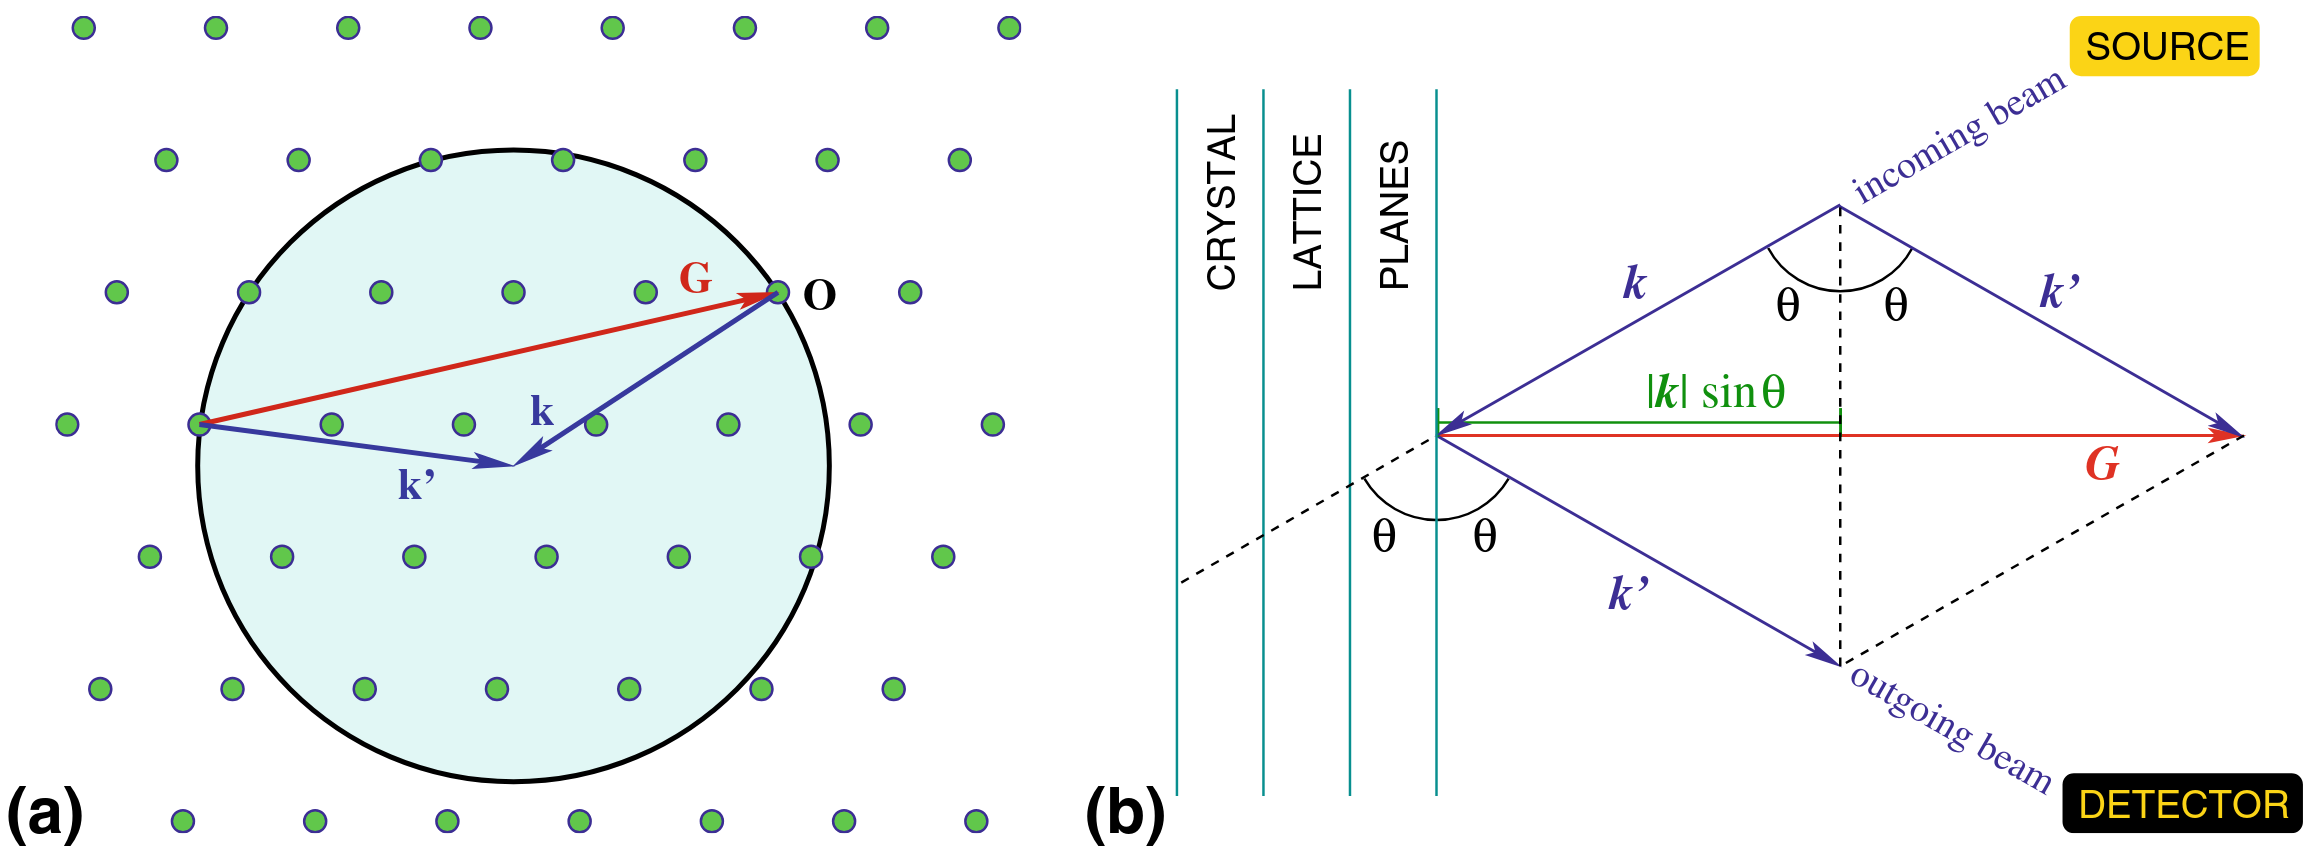
\includegraphics[width = 0.70 \textwidth]{diffr-e.png}
	\caption{Ewald construction.}
	\label{diffr-e}
\end{figure}

Come si vede in Fig. \ref{diffr-e}, vale la relazione $ \ve{k} \cdot \hat{\ve{G}} = - \sin \theta $, dove l'angolo di scattering tra $ \ve{k} $ e $ \ve{k}' $ è $ 2\theta $. Essendo i piani nel reticolo associati a $ \ve{G} $ separati da una distanza $ d = n \frac{2\pi}{\abs{\ve{G}}} $, dove $ n $ è il massimo comun divisore degli indici di Miller di $ \ve{G} $, ed valendo la relazione $ \abs{\ve{k}} = \frac{2\pi}{\lambda} $, dove $ \lambda $ è la lunghezzaq d'onda della radiazione incidente, si trova la \textit{condizione di Bragg} per la diffrazione:
\begin{equation}
	2 d \sin \theta = n \lambda
\end{equation}
Secondo questa equazione (e come confermato in Fig. \ref{diffr-e}), non avviene diffrazione per $ \lambda > 2d $. Nella pratica, per generare dei raggi diffratti da un singolo cristallo, si muove il reticolo reciproco rispetto alla sfera di Ewald fino a quando non ci sono almeno due punti che la intersecano: per fare ciò, o si varia la lunghezza d'onda incidente, andando a modificare il raggio della sfera di Ewald, o si ruota il cristallo (dato che il reticolo reciproco ruota della stessa quantità di quello reale). \\
Solitamente si studiano le \textit{polveri}, ovvero insiemi di microcristalli ruotati randomicamente nello spazio: la distribuzione uniforme di orientazioni equivale ad una media sulle possibili rotazioni del reticolo reciproco. Di conseguenza, nella costruzione della sfera di Ewald per una polvere, si possono considerare non solo i punti che intersecano la sfera, ma anche le intersezioni delle possibili rotazioni di tale sfera, ottenendo una maggiore possibilità di ottenere un pattern di diffrazione. \\
Infine, si noti che difetti e dimensione finita del cristallo pongono i picchi di Bragg su un background continuo diffuso: all'aumentare del disordine l'intensità del background cresce, fino a quando non sono più presenti picchi di Bragg (solidi amorfi, liquidi).

\section{Elettroni}

All'interno dei solidi, gli elettroni si muovo secondo l'equazione elettronica Eq. \ref{eq:mol-el-eq}: perciò, è possibile definire un potenziale adiabatico (Eq. \ref{eq:ad-pot}) che descrive il moto dei nuclei (Eq. \ref{eq:mol-nucl-eq}).

\subsection{Elettroni nei cristalli}

Nei solidi cristallini a basse temperature, il potenziale adiabatico la configurazione atomica in un intorno del minimo di potenziale, ovverosia mantiene i nuclei fissi nelle posizioni reticolari. Invocando la separazione adiabatica, dunque, si assume che i nuclei abbiano energia cinetica trascurabile e siano fissi nel reticolo, così da ridurre il problema a quello elettronico. \\
Innanzitutto, data la simmetria reticolare del cristallo, si ha che l'Hamiltoniana elettronica è invariante per le traslazioni discrete del reticolo:
\begin{equation}
	[\hat{\mathcal{H}} , \hat{T}_\ve{R}] = 0 \quad \forall \ve{R} \in \text{reticolo}
\end{equation}
Di conseguenza, le autofunzioni $ \phi(\ve{r}) $ dell'Hamiltoniana devono soddisfarre:
\begin{equation}
	\hat{T}_\ve{R} \phi(\ve{r}) = \alpha_\ve{R} \phi(\ve{r})
\end{equation}
con $ \alpha_\ve{R} \in \C $. Essendo il cristallo un sistema periodico, si deve poter applicare $ \hat{T}_\ve{R} $ un numero arbitrario di volte: se $ \abs{\alpha_\ve{R}} < 1 $ la densità di probabilità tende ad annullarsi, all'aumentare del numero di $ \hat{T}_\ve{R} $ applicati, mentre se $ \abs{\alpha_\ve{R}} > 1 $ tende a divergere. L'unica possibilità, dunque, è:
\begin{equation*}
	\abs{\alpha_\ve{R}} = 1
	\qquad \Rightarrow \qquad
	\alpha_\ve{R} = e^{-i \varphi_\ve{R}}
\end{equation*}
Un'altra proprietà che $ \hat{T}_\ve{R} $ deve soddisfare è la legge compositiva del gruppo:
\begin{equation*}
	\hat{T}_{\ve{R}_1} \hat{T}_{\ve{R}_2} = \hat{T}_{\ve{R}_1 + \ve{R}_2}
	\qquad \Rightarrow \qquad
	\varphi_{\ve{R}_1} \varphi_{\ve{R}_2} = \varphi_{\ve{R}_1 + \ve{R}_2}
\end{equation*}
Si può prendere WLOG $ \varphi_\ve{R} = \ve{q} \cdot \ve{R} $, con $ \ve{q} \in \R $, ma si noti che esso non è univocamente determinato: infatti, dall'Eq. \ref{eq:rec-ret}, si ha che:
\begin{equation*}
	e^{-i \ve{q} \cdot \ve{R}} = e^{-i (\ve{q} + \ve{G}) \cdot \ve{R}} \quad \forall \ve{G} \in \text{reticolo reciproco}
\end{equation*}
Ciò significa che $ \ve{q} $ è definito a meno di un qualsiasi vettore $ \ve{G} $ del reticolo reciproco. Questo permette di ridurre $ \ve{q} $ ad un vettore $ \ve{k} $ nella prima BZ scegliendo un opportuno $ \ve{G} $. La trattazione dell'intero cristallo è così ridotta alla sola prima BZ, e l'operatore traslazione agisce come:
\begin{equation}
	\hat{T}_\ve{R} \phi(\ve{r}) = \phi(\ve{r} - \ve{R}) = e^{-i \ve{k} \cdot \ve{R}} \phi(\ve{r})
	\label{eq:trasl-op}
\end{equation}

\begin{theorem}{Teorema di Bloch}{}
	In un reticolo cristallino, ogni funzione d'onda elettronica è un'onda piana modulata da una funzione periodica:
	\begin{equation}
		\phi(\ve{r}) = e^{i \ve{k} \cdot \ve{r}} u_\ve{k}(\ve{r})
		\qquad \qquad
		u_\ve{k}(\ve{r}) = u_\ve{k}(\ve{r} - \ve{R})
		\label{eq:bloch-th}
	\end{equation}

	\tcblower

	\begin{proof}
		Dall'Eq. \ref{eq:trasl-op}:
		\begin{equation*}
			\begin{split}
				\phi(\ve{r} - \ve{R})
				& = e^{-i \ve{k} \cdot \ve{R}} \phi(\ve{r}) \\
				& = e^{i \ve{k} \cdot (\ve{r} - \ve{R})} u_\ve{k}(\ve{r} - \ve{R}) = e^{-i \ve{k} \cdot \ve{R}} e^{i \ve{k} \cdot \ve{r}} u_\ve{k}(\ve{r}) = e^{-i \ve{k} \cdot \ve{R}} \phi(\ve{r})
			\end{split}
		\end{equation*}
	\end{proof}
\end{theorem}

È possibile esprimere la funzione periodica $ u_\ve{k}(\ve{r}) $ in serie di Fourier discreta:
\begin{equation}
	u_\ve{k}(\ve{r}) = \sum_\ve{G} c_{\ve{G},\ve{k}} e^{i \ve{G} \cdot \ve{r}}
	\qquad \Rightarrow \qquad
	\phi(\ve{r}) = \sum_\ve{G} c_{\ve{G},\ve{k}} e^{i (\ve{G} + \ve{k}) \cdot \ve{r}}
\end{equation}

\begin{proposition}{Equazione elettronica}{}
	L'equazione elettronica in un cristallo è:
	\begin{equation}
		\left[ -\frac{\hbar^2}{2m_e} (\nabla + i\ve{k})^2 + V_\text{eff}(\ve{r}) \right] u_{j,\ve{k}}(\ve{r}) = E_{j,\ve{k}} u_{j,\ve{k}}(\ve{r})
		\label{eq:lat-el-eq}
	\end{equation}
	con $ V_\text{eff} \equiv V_{ee} + V_{ne} $ nella prima BZ.

	\tcblower

	\begin{proof}
		Dall'Eqq. \ref{eq:mol-el-eq}-\ref{eq:bloch-th}, l'equazione elettronica può essere scritta nella prima BZ come:
		\begin{equation*}
			\left[ -\frac{\hbar^2}{2m_e} \nabla^2 + V_\text{eff}(\ve{r}) \right] e^{i \ve{k} \cdot \ve{r}} u_{j,\ve{k}}(\ve{r}) = E_{j,\ve{k}} e^{i \ve{k} \cdot \ve{r}} u_{j,\ve{k}}(\ve{r})
		\end{equation*}
		Il termine cinetico viene riscritto come:
		\begin{equation*}
			\begin{split}
				\nabla^2 \left[ e^{i \ve{k} \cdot \ve{r}} u_{j,\ve{k}}(\ve{r}) \right]
				& = \nabla \cdot \left[ e^{i \ve{k} \cdot \ve{r}} \nabla u_{j,\ve{k}}(\ve{r}) + i \ve{k} e^{i \ve{k} \cdot \ve{r}} u_{j,\ve{k}}(\ve{r}) \right] \\
				& = e^{i \ve{k} \cdot \ve{r}} \nabla^2 u_{j,\ve{k}}(\ve{r}) + 2 e^{i \ve{k} \cdot \ve{r}} i \ve{k} \cdot \nabla u_{j,\ve{k}}(\ve{r}) - \abs{\ve{k}}^2 e^{i \ve{k} \cdot \ve{r}} u_{j,\ve{k}}(\ve{r}) \\
				& = e^{i \ve{k} \cdot \ve{r}} (\nabla + i \ve{k})^2 u_{j,\ve{k}}(\ve{r})
			\end{split}
		\end{equation*}
		Questo dimostra la tesi.
	\end{proof}
\end{proposition}

L'equazione elettronica permette dunque di calcolare gli stati stazionari di qualsiasi elettrone nel cristallo, dato il suo vettore d'onda $ \ve{k} $, e permette di farlo risolvendo tale equazione all'interno di una singola cella (la prima BZ, con opportune condizioni al contorno periodiche), senza dover considerare l'intero volume del cristallo. \\
Si noti che l'Eq. \ref{eq:lat-el-eq}, a parte per lo shift immaginario dell'operatore $ \nabla $, è analoga all'usuale equazione di Schrödinger stazionaria: le soluzioni, dunque, saranno una serie di autofunzioni $ u_{j,\ve{k}}(\ve{r}) $, con $ j \in \N $, associate ad uno spettro di autovalori energetici crescenti $ E_{j,\ve{k}} $. \\
Tipicamente, l'Eq. \ref{eq:lat-el-eq} è risolta tramite una valutazione auto-consistente del potenziale di campo-medio $ V_\text{eff}(\ve{r}) $, trovando soluzioni numeriche per $ u_{j,\ve{k}}(\ve{r}) $ ed $ E_{j,\ve{k}} $ nella prima BZ (con condizioni al contorno periodiche).

\begin{figure}[!b]
	\centering
	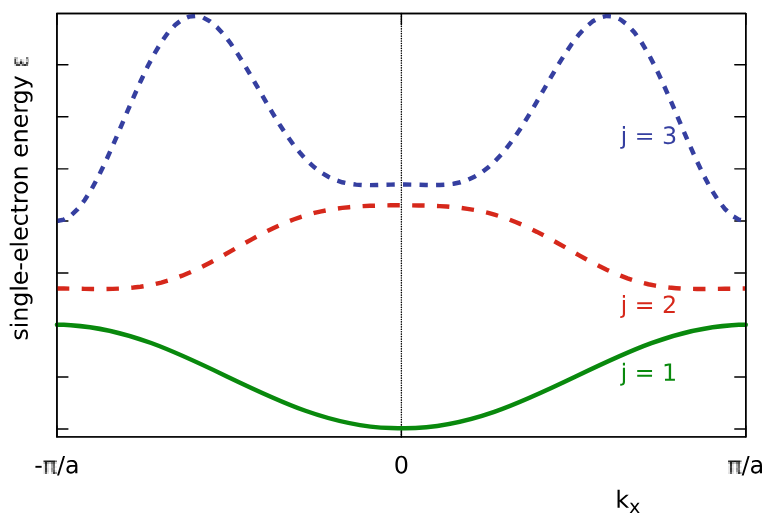
\includegraphics[width = 0.50 \textwidth]{en-band.png}
	\caption{First three energy bands for a 1D lattice.}
	\label{en-band}
\end{figure}

\subsection{Energy bands}

Facendo variare $ \ve{k} $ nella prima BZ, gli stati stazionari $ u_{j,\ve{k}}(\ve{r}) $ cambiano analiticamente con $ \ve{k} $, così da poter assumere una dipendenza liscia di $ u_{j,\ve{k}}(\ve{r}) $ da $ \ve{k} $. Di conseguenza, anche $ E_{j,\ve{k}} = E_j(\ve{k}) $ è una funzione liscia di $ \ve{k} $: per al variare di $ j \in \N $, si parla di \textit{energy bands}, in quanto fissato $ j \in \N $ gli autovalori $ E_j(\ve{k}) $ spannano un intervallo continuo di energie al variare di $ \ve{k} $ nella prima BZ. Come si vede in Fig. \ref{en-band}, i range spannati da due bands successive $ E_j(\ve{k} $ ed $ E_{j+1}(\ve{k}) $ possono sia sovrapporsi che rimanere separati: nel secondo caso, si parla di \textit{band gaps}. Si vede quindi che la principale conseguenza del teorema di Bloch è che lo spettro energetico degli elettroni in un solido cristallino è formato da energy bands continue separate da intervalli di energie proibite (band gaps): questo è un comportamento intermedio tra gli elettroni negli atomi (spettro discreto) e gli elettroni liberi (spettro continuo).

\subsubsection{Modello a onde piane}

Dato che all'interno del cristallo il potenziale nucleare $ V_{ne} $ è schermato dalla repulsione elettronica $ V_{ee} $, il potenziale effettivo $ V_\text{eff} $ è abbastanza piccolo (eccetto che vicino ai nuclei atomici) da poter approssimare gli autostati degli elettroni con quelli di particella libera. Questi sono gli autostati del momento lineare $ \ket{\ve{k}} : \hat{\ve{p}} \ket{\ve{k}} = \hbar \ve{k} \ket{\ve{k}} $ (opportunamente normalizzati come $ \braket{\ve{k} | \ve{k}'} = \delta_{\ve{k}, \ve{k}'} $), così da poter scrivere gli autostati elettronici come:
\begin{equation}
	\ket{\phi} = \sum_\ve{k} c_\ve{k} \ket{\ve{k}}
\end{equation}
L'equazione elettronica può quindi essere riscritta come (proiettando su $ \ket{\ve{k}} $):
\begin{equation}
	\sum_{\ve{k}'} \left[ \frac{\hbar^2 k^2}{2m_e} \delta_{\ve{k},\ve{k}'} + \braket{\ve{k} | V_\text{eff} | \ve{k}'} \right] c_{\ve{k}'} = E_\ve{k} \sum_{\ve{k}'} \delta_{\ve{k},\ve{k}'} c_{\ve{k}'}
\end{equation}
Per l'elemento di matrice del potenziale effettivo si trova:
\begin{equation}
	\braket{\ve{k} | V_\text{eff} | \ve{k}'} = \mathcal{N} \int \dd^3r\, e^{i (\ve{k}' - \ve{k}) \cdot \ve{r}} V_\text{eff}(\ve{r}) \eqdef \tilde{V}_\text{eff}(\ve{k} - \ve{k}')
\end{equation}
Essendo il potenziale periodico con stessa periodicità del reticolo cristallino, la sua trasformata di Fourier è in realtà una serie discreta sul reticolo reciproco: $ \tilde{V}_\text{eff}(\ve{k} - \ve{k}') $ si annulla a meno che $ \ve{k} - \ve{k}' = \ve{G} $. Ciò significa che la maggior parte degli elementi off-diagonal di $ V_\text{eff} $ si annullano: dato un $ \ve{k} $ nella prima BZ, il potenziale accoppia lo stato $ \ket{\ve{k}} $ solo a stati $ \ket{\ve{k}'} : \ve{k}' = \ve{k} - \ve{G} $, con $ \ve{G} $ nel reticolo reciproco. Trattando separatamente ciascun sottospazio a $ \ve{k} $ fissato (ovvero l'insieme $ \{\ket{\ve{k} + \ve{G}} : \ve{G} \in \text{reticolo reciproco}\} $), quindi, l'equazione elettronica può essere espressa come:
\begin{equation}
	\begin{bmatrix}
		\ddots & \vdots & \vdots & \vdots &  \\
		\dots & E_{\ve{k} + \ve{G}_1}^{(0)} + \tilde{V}_\text{eff}(\ve{0}) & \tilde{V}_\text{eff}(\ve{G}_1 - \ve{G}_2) & \tilde{V}_\text{eff}(\ve{G}_1 - \ve{G}_2) & \dots \\
		\dots & \tilde{V}_\text{eff}(\ve{G}_2 - \ve{G}_1) & E_{\ve{k} + \ve{G}_2}^{(0)} + \tilde{V}_\text{eff}(\ve{0}) & \tilde{V}_\text{eff}(\ve{G}_2 - \ve{G}_3) & \dots \\
		\dots & \tilde{V}_\text{eff}(\ve{G}_3 - \ve{G}_1) & \tilde{V}_\text{eff}(\ve{G}_3 - \ve{G}_2) & E_{\ve{k} + \ve{G}_3}^{(0)} + \tilde{V}_\text{eff}(\ve{0}) & \dots \\
		 & \vdots & \vdots & \vdots & \ddots
	\end{bmatrix}
	\begin{pmatrix}
		\vdots \\ c_{\ve{k} + \ve{G}_1} \\ c_{\ve{k} + \ve{G}_2} \\ c_{\ve{k} + \ve{G}_3} \\ \vdots
	\end{pmatrix}
	= E_\ve{k}
	\begin{pmatrix}
		\vdots \\ c_{\ve{k} + \ve{G}_1} \\ c_{\ve{k} + \ve{G}_2} \\ c_{\ve{k} + \ve{G}_3} \\ \vdots
	\end{pmatrix}
	\label{eq:mat-el-eq}
\end{equation}
dove l'energia all'ordine zero è quella dell'elettrone libero:
\begin{equation}
	E_\ve{k}^{(0)} = \frac{\hbar^2 k^2}{2m_e}
\end{equation}
L'Eq. \ref{eq:mat-el-eq} va diagonalizzata separatamente per ciascun $ \ve{k} $ nella prima BZ. La diagonalizzazione è banale nel caso di potenziale costante senza elementi off-diagonal $ \tilde{V}_\text{eff}(\ve{G} \neq \ve{0}) = 0 $: in tal caso, gli autostati energetici sono proprio le onde piane $ \ket{\ve{k} + \ve{G}_j} $, con autovalori energetici shiftati dal potenziale $ E_{j,\ve{k}} = E_{\ve{k} + \ve{G}_j}^{(0)} + \tilde{V}_\text{eff}(\ve{0}) $. \\
Nei cristalli reali, però, ci saranno molti termini off-diagonal non-nulli: in tal caso, gli autostati energetici sono combinazioni lineari delle onde piane $ \ket{\ve{k} + \ve{G}_j} $ e vengono trovati numericamente. \\
Un caso analiticamente affrontabile è quello di potenziale debole: precisamente, esso si verifica quando i termini off-diagonal sono piccoli rispetto alle separazioni diagonali, ovvero:
\begin{equation}
	\abs{\tilde{V}_\text{eff}(\ve{G}_1 - \ve{G}_2)} \ll \abs{E_{\ve{k} + \ve{G}_1}^{(0)} - E_{\ve{k} + \ve{G}_2}^{(0)}}
\end{equation}
In tale condizione, l'energia al prim'ordine è $ E_{j,\ve{G}}^{(1)} \approx E_{\ve{k} + \ve{G}_j}^{(0)} + \tilde{V}_\text{eff}(\ve{0}) $ e gli elementi off-diagonal determinano una piccola perturbazione al second'ordine:
\begin{equation}
	E_{j,\ve{k}}^{(2)} = E_{j,\ve{k}}^{(1)} + \sum_{\ell \neq j} \frac{\abs{\braket{\ve{k} + \ve{G}_j | V_\text{eff} | \ve{k} + \ve{G}_\ell}}^2}{E_{\ve{k} + \ve{G}_j}^{(0)} - E_{\ve{k} + \ve{G}_\ell}^{(0)}} = E_{j,\ve{k}}^{(1)} + \sum_{\ell \neq j} \frac{\abs{\tilde{V}_\text{eff}(\ve{G}_j - \ve{G}_\ell)}^2}{E_{\ve{k} + \ve{G}_j}^{(0)} - E_{\ve{k} + \ve{G}_\ell}^{(0)}}
\end{equation}
Questa correzione, però, non è applicabile nei punti in cui $ E_{\ve{k} + \ve{G}_j}^{(0)} \simeq E_{\ve{k} + \ve{G}_\ell}^{(0)} $ (evidenziati in Fig. \ref{band-par}): in questi punti, i termini off-diabonal diventano grandi e l'andamento risulta molto diverso da quello parabolico. Nei punti in cui due stati $ \ket{\ve{k} + \ve{G}_j} , \ket{\ve{k} + \ve{G}_\ell} $ diventano quasi degeneri, le band energies approssimate si possono calcolare diagonalizzando le (sotto)matrice:
\begin{equation*}
	\begin{bmatrix}
		E_{\ve{k} + \ve{G}_j}^{(0)} + \tilde{V}_\text{eff}(\ve{0}) & \tilde{V}_\text{eff}(\ve{G}_j - \ve{G}_\ell) \\
		\tilde{V}_\text{eff}(\ve{G}_\ell - \ve{G}_j) & E_{\ve{k} + \ve{G}_\ell}^{(0)} + \tilde{V}_\text{eff}(\ve{0})
	\end{bmatrix}
	\equiv
	\begin{bmatrix}
		E_{j,\ve{k}}^{(1)} & \Delta \\
		\Delta^* & E_{\ell,\ve{k}}^{(1)}
	\end{bmatrix}
\end{equation*}
Si trova che il coupling term $ \Delta $ induce una repulsione tra bande (formando gaps), le quali si trovano sempre a distanze energetiche pari o superiori a $ 2\abs{\Delta} = \abs{2\tilde{V}_\text{eff}(\ve{G}_j - \ve{G}_\ell} $, come riportato in Fig. \ref{band-gap}.

\begin{figure}
	\centering
	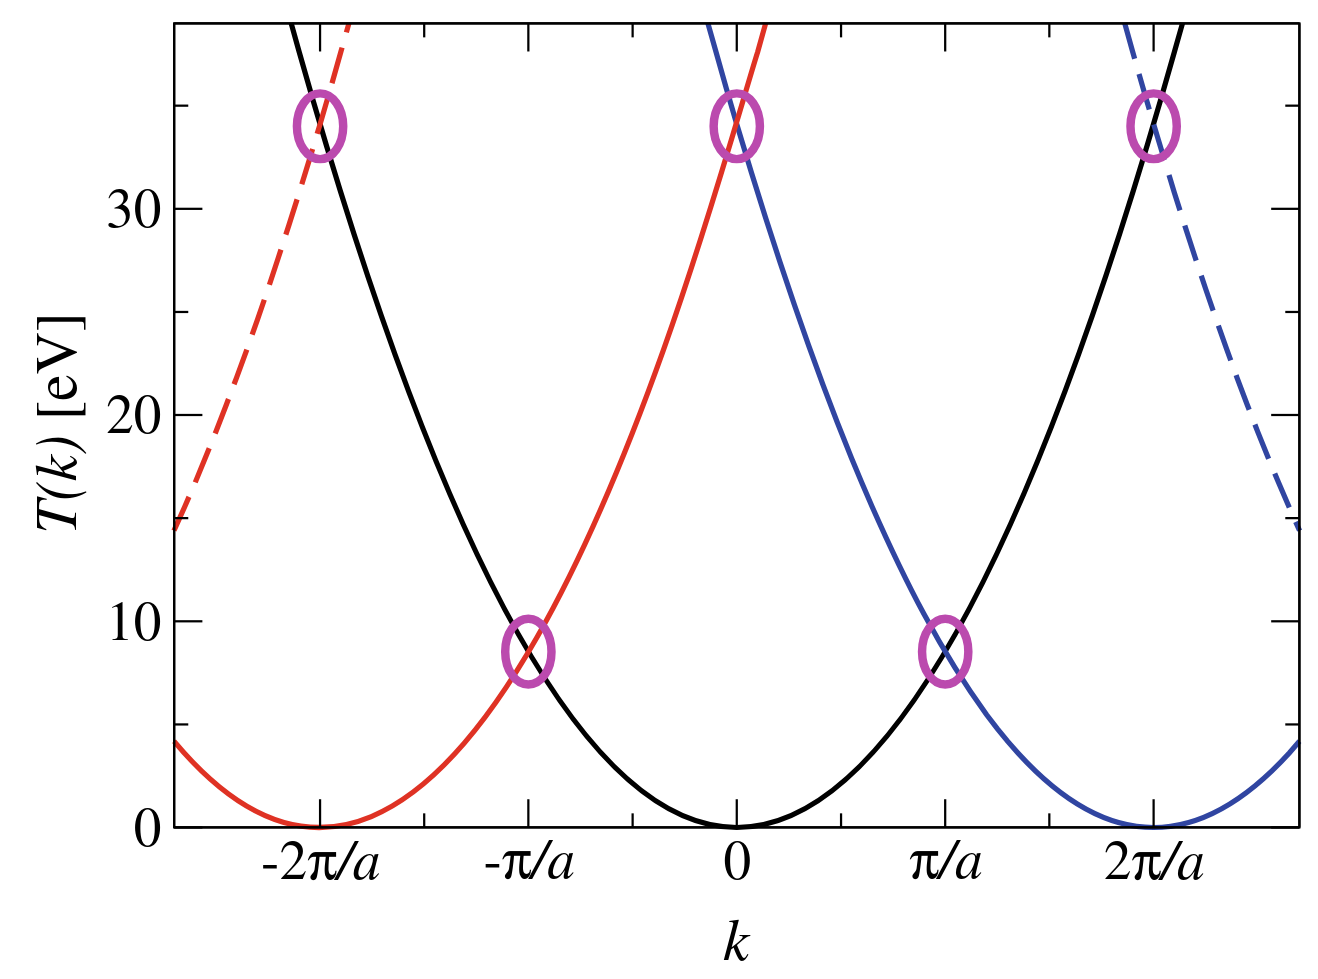
\includegraphics[width = 0.50 \textwidth]{band-par.png}
	\caption{1D free-electron parabolas $ E_{k + G_j}^{(0)} $, with $ G_j = \frac{2\pi}{a} j $: $ j = 0 $ in black, $ j = 1 $ in blue, $ j = 2 $ dashed in blue, $ j = -1 $ in red and $ j = -2 $ dashed in red.}
	\label{band-par}
\end{figure}
\begin{figure}
	\centering
	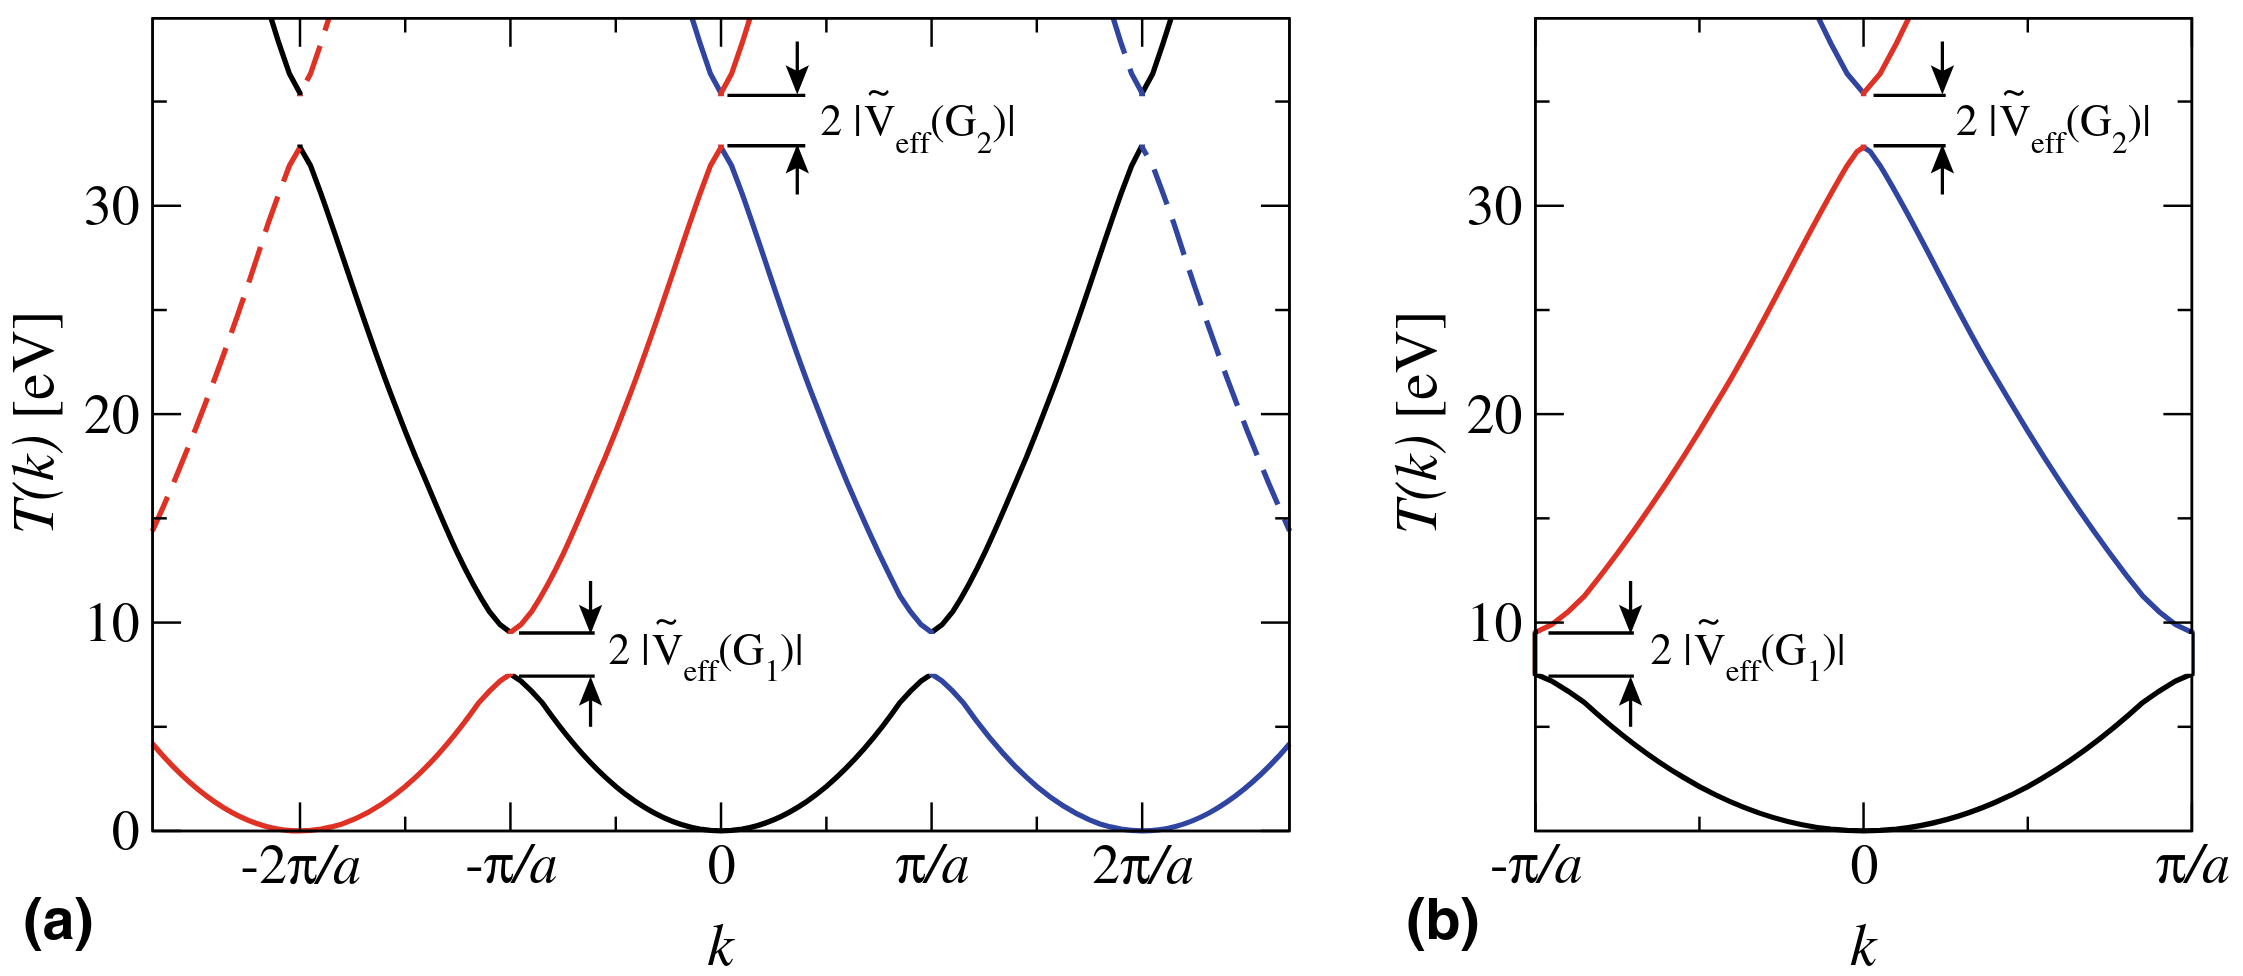
\includegraphics[width = 0.70 \textwidth]{band-gap.png}
	\caption{$ \abs{2\tilde{V}_\text{eff}(G_j)} $-wide gaps at each degeneracy point $ k = \frac{1}{2} G_j $, with the first BZ in detail.}
	\label{band-gap}
\end{figure}

Il modello a onde piane mostra chiaramente la formazione di band gaps, ovvero intervalli di energie proibite che separando le energy bands. In Fig. \ref{band-par}-\ref{band-gap} si vede come in 1D il potenziale periodico apre dei gap in tutti i punti $ k = \frac{1}{2} G $. In generale, in 3D, i gap si aprono in tutti i punti $ \ve{k} : \abs{\ve{k} + \ve{G}} = \abs{\ve{k}} $, per un qualche $ \ve{G} \in \text{reticolo reciproco} $: questa è proprio la condizione di Bragg per la diffrazione (Eq. \ref{eq:bragg-diffr}). Si noti che non sempre il potenziale periodico va a creare delle band gaps ben definite: può capitare, infatti, che un range di energie proibite per una certa direzione $ \ve{k} $ sia invece permessa per un'altra direzione $ \ve{k}' $. \\
Si vede che, nel modello a onde piane, l'indice $ j $ di una banda rappresenta semplicemente il numero di bande energeticamente sottostanti ad essa.

\subsubsection{Modello di Kronig-Penney}

\begin{figure}[!b]
	\centering
	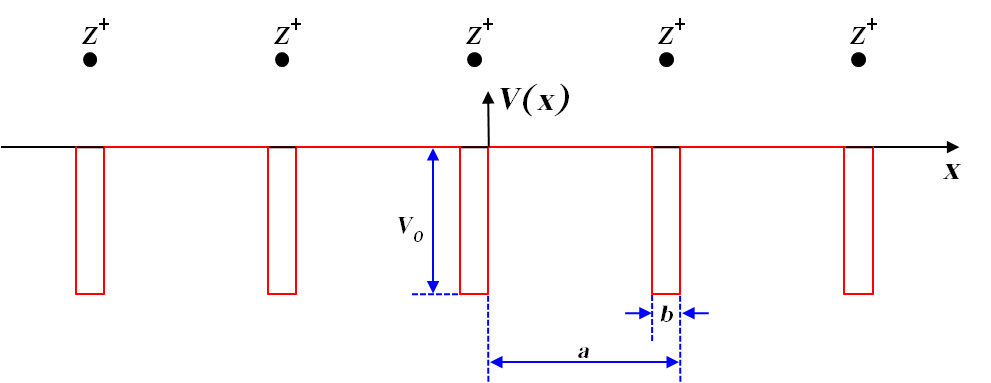
\includegraphics[width = 0.70 \textwidth]{kr-pen.png}
	\caption{Kronig-Penney model for the periodic potential.}
	\label{kr-pen}
\end{figure}

Una trattazione diversa è possibile grazie al modello di Kronig-Penney per il potenziale periodico. Grazie alle condizioni di periodicità, si può restringere la trattazione alla cella primaria, e nel caso 1D vale:
\begin{equation}
	V(x) =
	\begin{cases}
		-V_0 & -b < x < 0 \\
		0 & 0 < x < a-b
	\end{cases}
\end{equation}
La trattazione è analoga a quella della particella in una buca finita di potenziale, ma con diverse condizioni al contorno. In particolare, per un elettrone di energia $ E $, si trova:
\begin{equation}
	\psi(x) =
	\begin{cases}
		A e^{i \alpha x} + B e^{-i \alpha x} & -b < x < 0 \\
		C e^{i \beta x} + D e^{-i \beta x} & 0 < x < a-b
	\end{cases}
\end{equation}
con:
\begin{equation}
	\alpha^2 \equiv \frac{2m (E + V_0)}{\hbar^2}
	\qquad \qquad
	\beta^2 \equiv \frac{2m E}{\hbar^2}
\end{equation}
Si devono imporre condizioni di raccordo e periodicità, ovvero:
\begin{equation}
	\psi(0^-) = \psi(0^+)
	\qquad \qquad
	\psi'(0^-) = \psi'(0^+)
\end{equation}
\begin{equation}
	\psi(-b) = \psi(a-b)
	\qquad \qquad
	\psi'(-b) = \psi'(a-b)
\end{equation}
Dal teorema di Bloch $ \psi(x) = e^{ikx} u_k(x) $, dunque imponendo le condizioni periodiche si trova la condizione:
\begin{equation}
	\cos (ka) = \cos(\beta b) \cos (\alpha(a-b)) - \frac{\alpha^2 + \beta^2}{2\alpha \beta} \sin(\beta b) \sin(\alpha (a-b))
\end{equation}
Prendendo il limite di queste barriere di potenziale a $ \delta $ di Dirac, ovvero $ b \rightarrow 0 , V_0 \rightarrow \infty : bV_0 = \text{const.} $, si trova:
\begin{equation}
	\cos(ka) = \cos(\alpha a) + p \sinc(\alpha a)
	\qquad \qquad
	p \equiv \frac{m V_0 ba}{\hbar^2}
\end{equation}
Questa equazione ha soluzione solo se $ \abs{\cos(\alpha a) + p \sinc(\alpha a)} \le 1 $: essendo $ \alpha a \propto \sqrt{E} $, ciò significa che ci sono dei valori energetici per cui non c'è soluzione, ovvero si formano delle band gaps (Fig. \ref{kr-pen-en}).

\begin{figure}
	\centering
	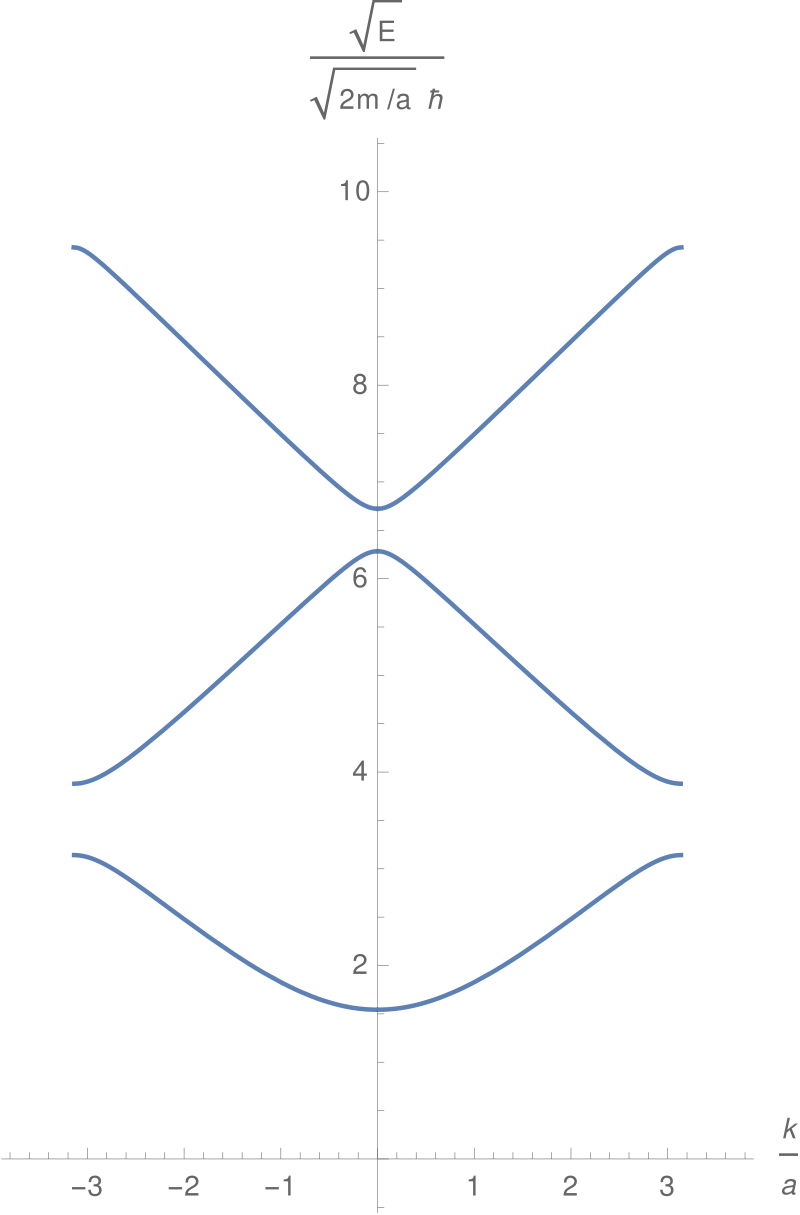
\includegraphics[width = 0.30 \textwidth]{kr-pen-en.png}
	\caption{Energy bands for the Kronig-Penney model.}
	\label{kr-pen-en}
\end{figure}

\subsubsection{Tight-binding model}

Si consideri un reticolo cristallino 1D con atomi posizionati in punti equispaziati $ t_n \equiv na $: vicino ciascuno di essi, il potenziale effettivo sarà approssimato da quello di un singolo nucleo isolato, dunque è possibile ottenere la funzione d'onda elettronica a partire da quelle atomiche. In questo modo, le funzioni d'onda di Bloch sono delle generalizzazioni degli orbitali leganti/anti-leganti ottenuti tramite LCAO (si pensa al solido come ad una grossa molecola): questo sistema è appropriato per elementi che contengono solo orbitali $ \text{s} $, mentre risulta poco adatto a descrivere stati metallici estesi. \\
Si considerino le funzioni d'onda atomiche per ciascun atomo $ \phi_\text{a}(x-t_n) $. Essendo il sistema invariante per traslazioni, gli elementi diabonali di matrice dell'Hamiltoniana sono tutti uguali:
\begin{equation}
	\braket{\phi_\text{a}(x-t_n) | \mathcal{H} | \phi_\text{a}(x-t_n)} = E_0
\end{equation}
Si definisce inoltre l'\textit{integrale di Hopping}:
\begin{equation}
	\gamma \defeq \braket{\phi_\text{a}(x-t_n) | \mathcal{H} | \phi_\text{a}(x-t_{n+1})}
\end{equation}
Essendo i potenziali atomici attrattivi, si ha $ \gamma < 0 $. Per costruire una funzione d'onda periodica estesa a partire da questi orbitali atomici localizzati, si può utilizzare il teorema di Bloch, trovando la \textit{somma di Bloch}:
\begin{equation}
	\phi_k(x) = \frac{1}{\sqrt{N}} \sum_{n = 1}^N e^{i k t_n} \phi_\text{a}(x-t_n)
\end{equation}
Si vede infatti che $ \phi_k(x+a) = e^{ika} \phi_k(x) $, rispettando il teorema di Bloch. Lo spettro energetico sarà:
\begin{equation}
	E(k) = \braket{\phi_k | \mathcal{H} | \phi_k} = E_0 + 2 \gamma \cos(ka)
\end{equation}
Attorno al minimo si recupera la forma parabolica:
\begin{equation}
	E(k) \simeq E_0 + 2\gamma - \gamma a^2 k^2 \equiv E_0 + 2\gamma + \frac{\hbar^2 k^2}{2\mu}
	\qquad \qquad
	\mu \equiv \frac{\hbar^2}{2 \abs{\gamma} a^2}
\end{equation}
dove si è definita la massa efficace $ \mu $. Si vede che $ \mu $ è piccola per $ \abs{\gamma} $ grande: le masse piccole sono più soggette ai campi esterni (in quanto accellerano più facilmente).

\subsection{Riempimento delle bande}

\begin{figure}
	\centering
	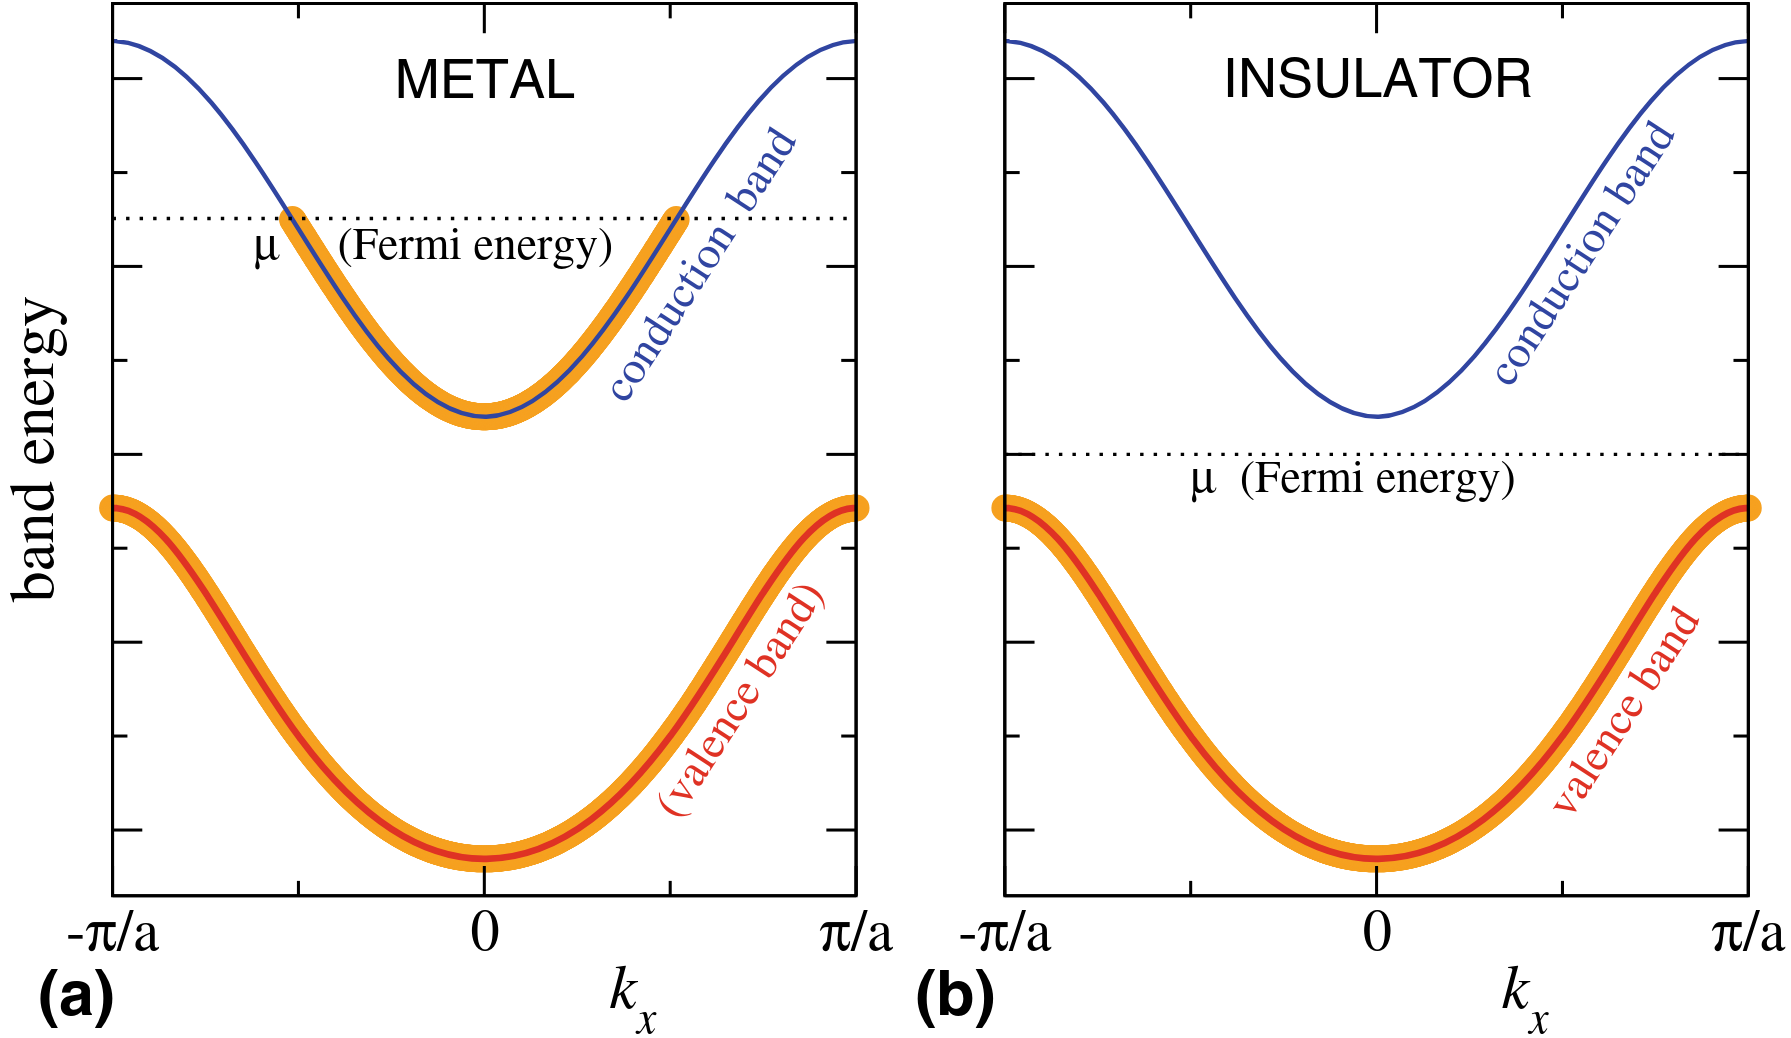
\includegraphics[width = 0.50 \textwidth]{met-ins.png}
	\caption{The two fundamental $ T = 0 $ band-fillinf schemes: metal and insulator.}
	\label{met-ins}
\end{figure}

Il ground state ($ T = 0 $) di un sistema di elettroni indipendenti in un potenziale periodico si ottiene riempiendo gli stati single-particle nelle energy bands fino all'energia di Fermi $ \mu $, come nel modello a fermioni liberi. \\
In base al numero di elettroni nel solido, l'energia di Fermi può intersecare una o più energy bands o capitare in mezzo ad una band gap (vedere Fig. \ref{met-ins}): nel primo caso, gli elettroni nelle band occupate parzialmente possono acquisire energia d'eccitazione da campi esterni, così accellerando e conducendo corrente elettrica (\textit{metallo}); nel secondo caso, invece, gli elettroni in una band completa rimangono congelati per il principio d'esclusione, e le eccitazioni richiedono energie dell'ordine della band gap (\textit{isolante}). In generale, l'energy band completamente riempita più alta viene detta \textit{banda di valenza}, mentre quella parzialmente riempita più bassa \textit{banda di conduzione}. \\
Per capire come si distribuiscono gli elettroni nelle energy bands, si consideri una porzione di cristallo di volume $ V = N_1 N_2 N_3 V_c $, la quale si estende per $ N_1 / N_2 / N_3 $ periodi nella direzione $ \ve{a}_1 / \ve{a}_2 / \ve{a}_3 $. Applicando la condizione di periodicità $ \psi-{j,\ve{k}}(\ve{r}) = \psi_{j,\ve{k}}(\ve{r} + N_i \ve{a}_i) $ si trova:
\begin{equation*}
	\ve{k} = \frac{n_1}{N_1} \ve{b}_1 + \frac{n_2}{N_2} \ve{b}_2 + \frac{n_3}{N_3} \ve{b}_3
	\qquad \qquad
	n_i = - \frac{N_i}{2} + 1 , - \frac{N_i}{2} + 2 , \dots , \frac{N_i}{2} -1 , \frac{N_i}{2}
\end{equation*}
I valori possibili di $ \ve{k} $ sono quindi $ N = N_1 N_2 N_3 $: questi diventano densi e riempiono la prima BZ nel limite $ N_i \rightarrow \infty $ (cristallo ideale infinito). Ciascuno stato nella banda $ j $ può ospitare due elettroni (degenerazione da spin), dunque in totale la banda ha $ 2N $ stati single-particle.

\begin{proposition}{Occupazione delle bande}{}
	Detto $ m $ il numero di elettroni in ciascun atomo ed $ n_c $ il numero di atomi per cella, il numero di bande occupate è $ \frac{1}{2} m n_c $.

	\tcblower

	\begin{proof}
		Essendo presenti $ N $ celle nel volume $ V $, il numero totale di atomi in $ V $ è $ m n_c N $: ciascuna banda può ospitare $ 2N $ elettroni, dunque il numero di bande occupate è $ \frac{m n_c N}{2N} = \frac{1}{2} m n_c $.
	\end{proof}
\end{proposition}

Si hanno dunque due possibili casi, a seconda che il numero di elettroni per cella $ m n_c $ sia pari o dispari (vedere Fig. \ref{ne-na}):
\begin{itemize}
	\item $ m n_c $ pari: viene occupato un numero intero di bande, ovvero la banda di conduzione è vuota;
	\item $ m n_c $ dispari: l'ultima banda è semi-piena, ovvero ci sono degli elettroni nella banda di conduzione.
\end{itemize}

\begin{figure}
	\centering
	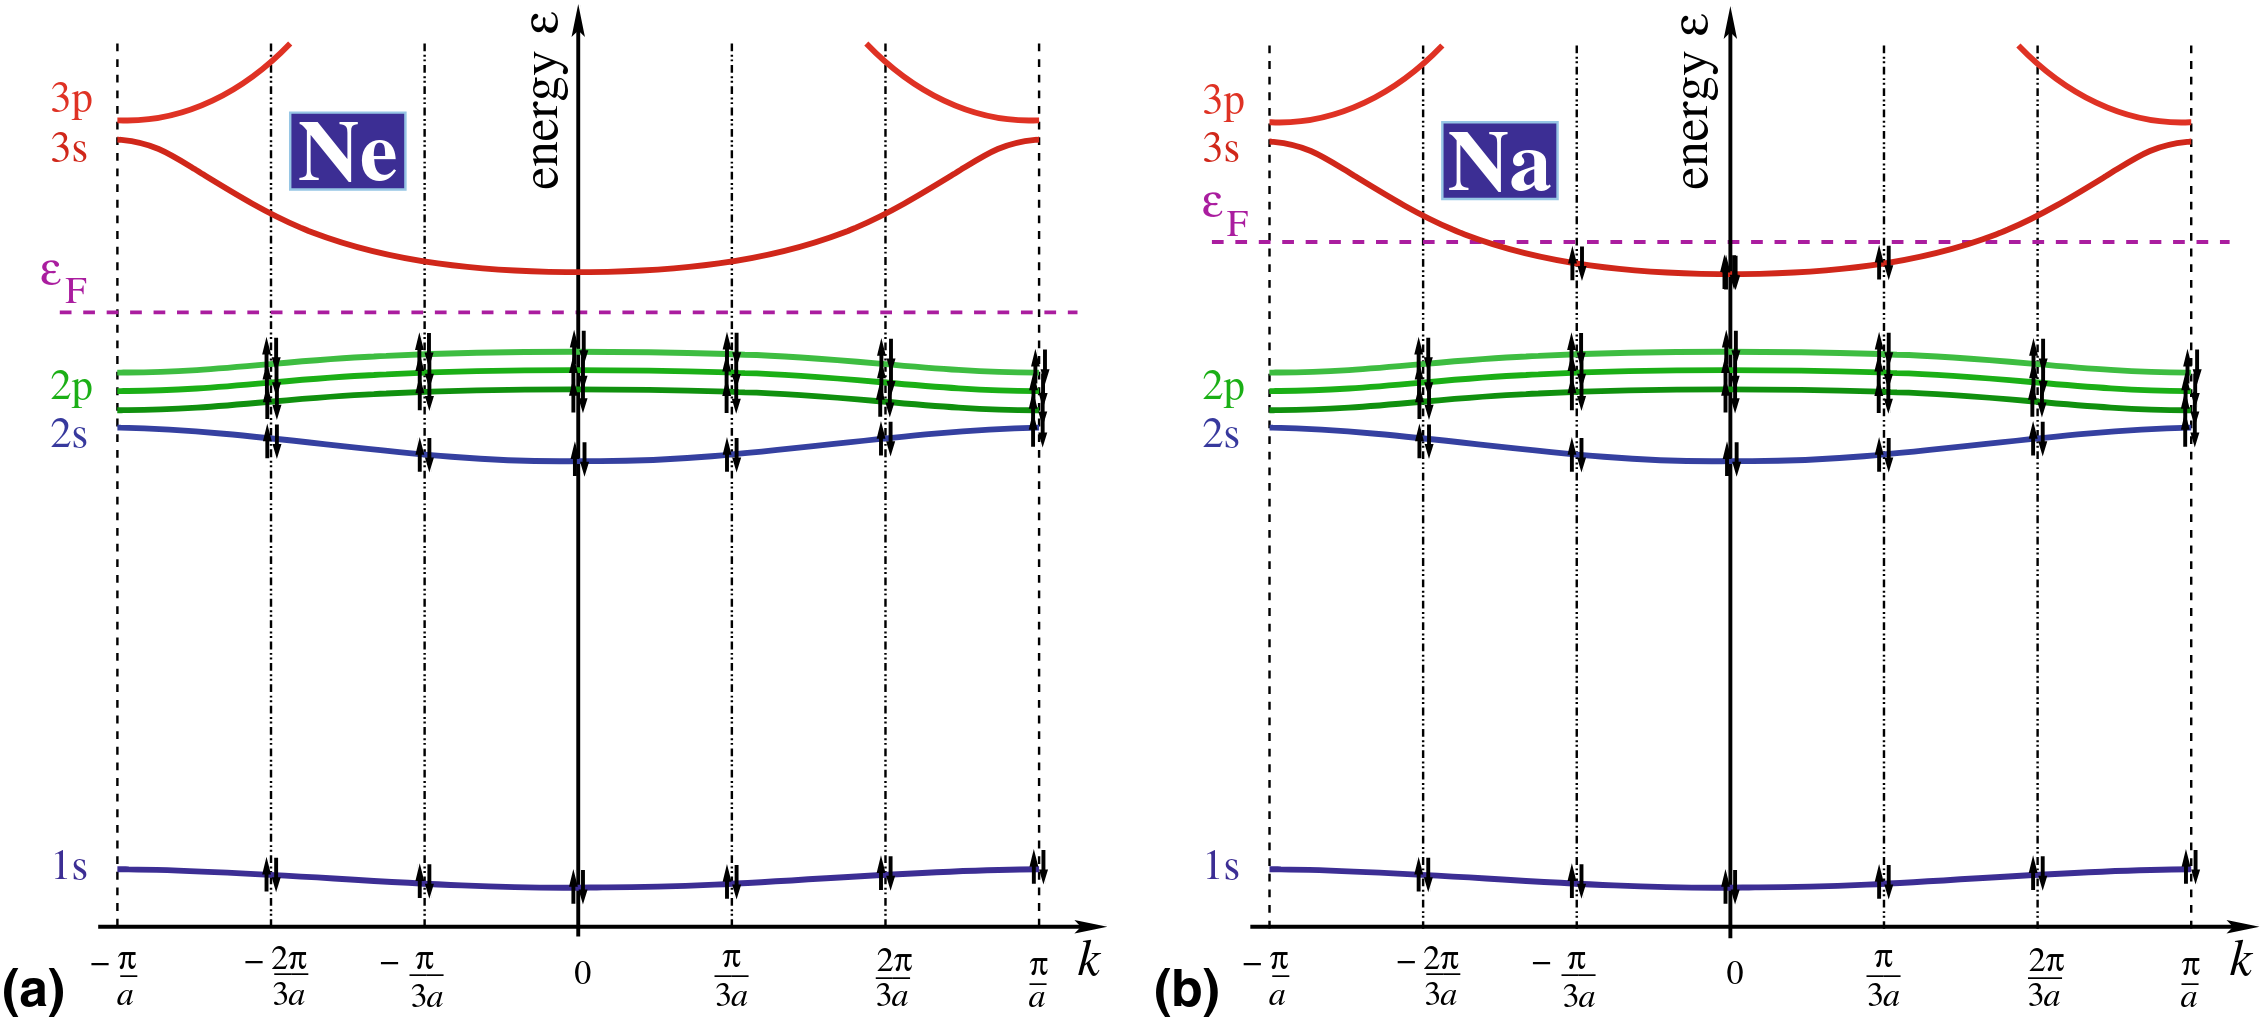
\includegraphics[width = 0.70 \textwidth]{ne-na.png}
	\caption{Filling of bands for 1D crystals of $ N = 6 $ atoms of $ \ch{Ne} $ and $ \ch{Na} $.}
	\label{ne-na}
\end{figure}

Si vede dunque che i cristalli con un numero dispari di elettroni per cella sono dei metalli, mentre quelli che ne hanno un numero pari possono essere sia isolanti che metalli: quest'ultimo caso si verifica quando la banda di valenza e quella di conduzione non sono separate da gap, dunque parte della banda di valenza è al di sopra dell'energia di Fermi e parte della banda di conduzione al di sotto di essa (si verifica nel gruppo 2 (metalli alcalino-terrosi) e nel gruppo 12 ($ \ch{Zn} $, $ \ch{Cd} $ e $ \ch{Hg} $)).

\subsubsection{Metalli}

I metalli presentano una particolare capacità di condurre corrente elettrica\footnotemark: in particolare, mostrano una conducibilità elettrica che decresce con $ T $.
A $ T = 0 $, la \textit{superficie di Fermi} $ E = \mu $ separa gli stati pieni da quelli vuoti nello spazio reciproco (dei $ \ve{k} $), generalizzando la sfera di Fermi per il gas ideale di fermioni.

\footnotetext{In realtà tutti i solidi possono condurre corrente elettrica: ciò che caratterizza i metalli è l'andamento decrescente della conducibilità elettrica all'aumentare della temperatura, a differenza della (piccola) conducibilità elettrica degli isolanti che invece aumenta con $ T $.}

Adottando un approccio semiclassico, si può studiare il moto degli elettroni rappresentandoli come pacchetti d'onda, ovvero sovrapposizioni di stati di Bloch relativi ad una stessa banda $ j $. Il moto di un pacchetto d'onda soggetto ad un campo elettromagnetico esterno è governato da:
\begin{equation}
	\dot{\ve{r}} \equiv \ve{v}_j(\ve{k}) = \frac{1}{\hbar} \nabla_\ve{k} E_{j,\ve{k}}
	\label{eq:met-1}
\end{equation}
\begin{equation}
	\hbar \dot{\ve{k}} = -q_e \left[ \ve{E}_\text{ext}(t,\ve{r}) + \ve{v}_j(\ve {k}) \times \ve{B}_\text{ext}(t,\ve{r}) \right]
	\label{eq:met-2}
\end{equation}
dove si assume che il campo esterno vari lentamente nel tempo sulla scala della grandezza del pacchetto (tipicamente molto maggiore della dimensione della cella primaria del reticolo, in quanto si suppone il pacchetto centrato in un valore di del numero d'onda ben definito). \\
La velocità $ \ve{v}_j $ è la velocità del centro di massa dell'elettrone, ovvero la velocità di gruppo del wave-packet: l'Eq. \ref{eq:met-1} esprime il fatto che un pacchetto d'onda con relazione di dispersione $ \omega = \omega(\ve{k}) $ ha una velocità di gruppo $ \ve{v}_g = \nabla_\ve{k} \omega(\ve{k}) $, dato che per l'elettrone $ \omega(\ve{k}) = \frac{1}{\hbar} E_{j,\ve{k}} $ (si noti che per l'elettrone libero $ E_{j,\ve{k}} = \hbar^2 k^2 / (2m_e) $, quindi si trova giustamente $ \ve{v}_j(\ve{k}) = \hbar \ve{k} / m_e $). \\
L'Eq. \ref{eq:met-2} ricorda l'equazione classica per una particella carica in un campo elettromagnetico esterno (forza di Lorentz): il potenziale periodico del cristallo induce una dipendenza non-banale $ \ve{v}_j = \ve{v}_j(\ve{k}) $, dunque il \textit{momento cristallino} $ \hbar \ve{k} $ non rappresenta il momento reale dell'elettrone\footnotemark. Ciò nonostante, $ \ve{k} $ è comunque una costante del moto, dunque continua ad essere un buon numero quantico.

\footnotetext{Il momento cristallino non è autovalore dell'operatore $ -i \hbar \nabla_\ve{r} $, dato che:
\begin{equation*}
	-i \hbar \nabla_\ve{r} \left[ e^{i \ve{k} \cdot \ve{r}} u_\ve{k}(\ve{r}) \right] = \hbar \ve{k} e^{i \ve{k} \cdot \ve{r}} u_\ve{k}(\ve{r}) -i \hbar e^{i \ve{k} \cdot \ve{r}} \nabla_\ve{r} u_\ve{k}(\ve{r}) \neq \hbar \ve{k} e^{i \ve{k} \cdot \ve{r}} u_\ve{k}(\ve{r})
\end{equation*}
Prendendo il valore d'aspettazione, si vede che il momento dell'elettrone è il momento cristallino diminuito di una quantità che può essere vista come un momento medio efficace: quest'ultimo viene interpretato come un momento medio trasferito dall'elettrone al cristallo.
}

È possibile calcolare l'accellerazione di un elettrone, a partire dall'Eq. \ref{eq:met-1}:
\begin{equation*}
	\frac{\dd^2 \ve{r}}{\dd t^2} = \frac{\dd \ve{k}}{\dd t} \cdot \nabla_\ve{k} \ve{v}_j(\ve{k}) = \frac{1}{\hbar^2} \sum_{\alpha,\beta = 1}^3 \hat{\ve{e}}_\alpha \frac{\pa^2 E_{j,\ve{k}}}{\pa k_\alpha \pa k_\beta} \frac{\dd (\hbar k_\beta)}{\dd t} \equiv \sum_{\alpha,\beta = 1}^3 \hat{\ve{e}}_\alpha [m_\text{eff}^{-1}]_{\alpha,\beta} F_\beta
\end{equation*}
dove sono state definite la forza totale esterna agente sull'elettrone $ \ve{F} = \hbar \dot{\ve{k}} $ (Eq. \ref{eq:met-2}) e la \textit{massa efficace} $ m_\text{eff} $, definita tensorialmente tramite il suo inverso:
\begin{equation}
	[m_\text{eff}^{-1}]_{\alpha,\beta} = \frac{1}{\hbar^2} \frac{\pa^2 E_{j,\ve{k}}}{\pa k_\alpha \pa k_\beta}
\end{equation}
Questa massa può anche essere negativa o divergere, e per l'elettrone libero si trova correttamente $ m_\text{eff} = m_e $. In particolare, sulla superficie di Fermi (dove avviene il moto), gli elettroni si comportano come se avessero massa $ m_\text{eff} $ (opportuna media sulle componenti del tensore), la quale è proporzionale alla curvatura dell'energy band.

\paragraph{Corrente elettrica}

Con l'approccio semiclassico, è facile vedere che un'energy band completamente piena non conduce corrente. Essendo la densità di corrente trasportata da un wave-packet $ \ve{j}_p(\ve{k}) = -q_e \ve{v}_j(\ve{k}) / V $ e ricordando l'Eq. \ref{eq:dens-k}, si trova:
\begin{equation*}
	\ve{J} = \int_\text{BZ} \dd^3k\, \ve{j}_p(\ve{k}) g_s g(\ve{k}) = - \frac{q_e}{4\pi^3 \hbar} \int_\text{BZ} \dd^3k\, \nabla_\ve{k} E_{j,\ve{k}} = \ve{0}
\end{equation*}
che si annulla poiché è l'integrale sul periodo del gradiente di una funzione periodica. Ciò spiega perché non si osserva un aumento della conducibilità elettrica negli elementi cristallini all'aumentare di $ Z $: ad esempio, $ \ch{Cu} $, $ \ch{Ag} $ ed $ \ch{Au} $ hanno conducibilità simili, nonostante il numero totale di elettroni molto diverso. \\
Concentrandosi sulle bande semi-piene, si noti che gli stati di Bloch sono stati stazionari in un cristallo perfetto: di conseguenza, se un wave-packet ha velocità di gruppo finita ($ \nabla_\ve{k} E_{l,\ve{k}} \neq \ve{0} $), allora essa rimarrà immutata mentre l'elettrone si sposta nel cristallo. Ciò significa che, nell'approccio semiclassico, le correnti si dovrebbero propagare nel metallo come fossero nel vuoto, anche in assenza di un campo elettrico esterno: queste persistent current non vengono però osservate negli esperimenti.
Inoltre, secondo l'Eq. \ref{eq:met-2}, sotto l'effetto di un campo elettrico costante uniforme l'elettrone ha un moto ciclico nella prima BZ (ricordando le condizioni periodiche, si veda Fig. \ref{k-cycle}): queste sono note come \textit{oscillazioni di Bloch}. Di conseguenza, per l'Eq. \ref{eq:met-1}, la velocità è oscillante e genera correnti positive e negative per lo stesso periodo di tempo: ciò significa, che applicando un campo elettrico DC ad un filo metallico, si dovrebbe osservare una corrente AC. Questa è un'altra discrepanza con quanto viene osservato, in quanto la risposta dei metalli ad un campo elettrico esterno è dettata dalla legge di Ohm: $ \ve{J} = \sigma \ve{E} $, con $ \sigma $ conducibilità elettrica. \\
Queste discrepanza tra teoria semiclassica e realtà sono dovute al fatto che gli elettroni di Bloch, rappresentati da pacchetti d'onda, posti in un cristallo ideale possono muoversi all'infinito, senza dispersione d'energia. I cristalli reali, però, deviano da quelli ideali per la presenza di difetti e per il fatto che gli atomi non sono fissi nelle posizioni reticolari, ma possono oscillare attorno ad esse: ciò determina che gli elettroni di conduzione siano soggetti a fenomeni di scattering, in particolare a causa dell'interazione elettrone-fonone.

\begin{figure}
	\centering
	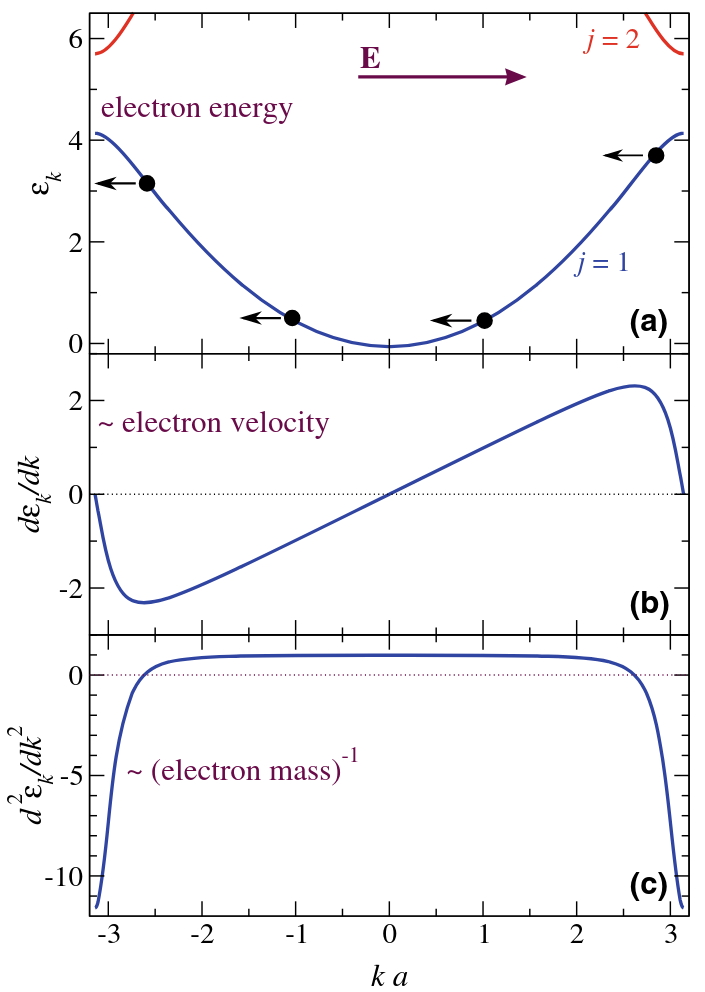
\includegraphics[width = 0.40 \textwidth]{k-cycle.png}
	\caption{Motion of an electron in the reciprocal lattice of a 1D crystal, under the action of a constant uniform electric field.}
	\label{k-cycle}
\end{figure}

Per metalli cristallini, il tempo medio $ \tau $ tra due collissioni di un elettrone (\textit{tempo libero medio} o tempo di rilassamento) è dell'ordine $ \tau \sim 10^{-13} \,\text{s} $, troppo breve perché l'elettrone raggiunga il bordo della prima BZ e mostri oscillazioni di Bloch\footnotemark.

\footnotetext{Per osservare le oscillazioni di Bloch servirebbe un cristallo estremamente puro a temperatura molto bassa, condizioni difficilmente ottenibili. In alternativa, si possono considerare i \textit{super-reticoli}, ovvero reticoli sovrapposti di materiali diversi, le cui celle si vanno ad alternare: ciò permette di rendere la cella primitiva più grande, ovvero di rimpicciolire la prima BZ. Si noti che sono necessari materiali tali per cui all'interfaccia non ci sia una grossa differenza di passi reticolari, così da non introdurre difetti.}

Mentre il campo elettrico esterno spinge gli elettroni ad occupare stati nella direzione di $ -q_e \ve{E}_\text{ext} $, le collisioni con difetti del cristallo e fononi tendono a riportare gli elettroni verso gli stati occupati all'equilibrio termico: dopo un transiente, l'effetto di $ \ve{E}_\text{eff} $ viene ridotto ad un piccolo shift $ \delta \ve{k} $ costante della superficie di Fermi rispetto alla sua configurazione all'equilibrio. Definendo $ \delta^3k $ il volume tra la superficie di Fermi all'equilibrio e quella shiftata, si può stimare la densità di corrente indotta da $ \ve{E}_\text{eff} $ come:
\begin{equation*}
	\ve{J} = - \frac{q_e}{4\pi^3} \int_{\delta^3k} \dd^3k\, \ve{v}_j(\ve{k}) \simeq - q_e \int_{\delta^3k} \dd^3k\, \hat{\ve{E}}_\text{ext} v_\text{F} \simeq -q_e v_\text{F} \hat{\ve{E}}_\text{eff} \delta^3k
\end{equation*}
dove si è approssimato l'integrale con la velocità di Fermi nella direzione del campo poiché sono coinvolti solo gli \textit{elettroni attivi}, ovvero quelli sulla superficie di Fermi. Osservando che nel tempo libero medio $ \tau $ l'elettrone varia il suo numero d'onda come $ \delta\ve{k} = -q_e \tau \ve{E}_\text{ext} / \hbar $ (Eq. \ref{eq:met-2}), si può stimare:
\begin{equation*}
	\delta^3k \simeq - \abs{\delta\ve{k}} k_\text{F}^2 \simeq - q_e \frac{\tau}{\hbar} \abs{\ve{E}_\text{ext}} k_\text{F}^2
\end{equation*}
dove il segno negativo indica che lo shift è opposto ad $ \ve{E}_\text{ext} $. Essendo $ v_\text{F} \simeq \hbar k_\text{F} / m_\text{eff} $ e ricordando l'Eq. \ref{eq:k-f}, si trova:
\begin{equation*}
	\ve{J} \simeq \frac{q_e^2 \tau}{m_e} \hat{\ve{E}}_\text{ext} \abs{\ve{E}_\text{ext}} k_\text{F}^3 \simeq \frac{q_e^2 \tau}{m_e} \frac{N}{V} \ve{E}
\end{equation*}
Ciò non è altro che la legge di Ohm con conducibilità elettrica pari a:
\begin{equation}
	\sigma = \frac{q_e^2 \tau}{m_e} \frac{N}{V}
\end{equation}
Grandezze tipiche sono $ \tau \sim 10^{-13} \,\text{s} $, $ v_\text{F} \sim 10^6 \,\text{m}/\text{s} $ e $ N/V \sim 10^{29} \,\text{m}^{-3} $: si stima dunque il cammino libero medio $ l \simeq \tau v_\text{F} \sim 100 \,\text{nm} $. All'aumentare della temperatura si osserva un aumento della resistivistà $ \rho = \sigma^{-1} $, ovvero una diminuzione del tempo libero medio $ \tau $: le collisioni diventano più frequenti quando il moto termico determina grandi spostamenti dei nuclei dalla loro posizione d'equilibrio\footnote{Il tempo libero medio è inversamente proporzionale al numero di fononi: $ \tau^{-1} \propto \sum_\varepsilon [n_\varepsilon]_\text{B} $. Ad energie termiche $ k_\text{B} T $ molto al di sopra dell'energia caratteristica dei fononi ($ \varepsilon \lesssim 100 \,\text{meV} $), il numero totale di fononi è lineare in $ T $: dall'Eq. \ref{eq:fer-dir-bos-ein} $ [n_\varepsilon]_\text{B} = (e^{\beta \varepsilon} - 1)^{-1} \simeq (\beta \varepsilon)^{-1} = k_\text{B} T / \varepsilon $. Di conseguenza, ad alte tempreature la resistività è lineare in $ T $, fatto osservato sperimentalmente.}.

\begin{figure}
	\centering
	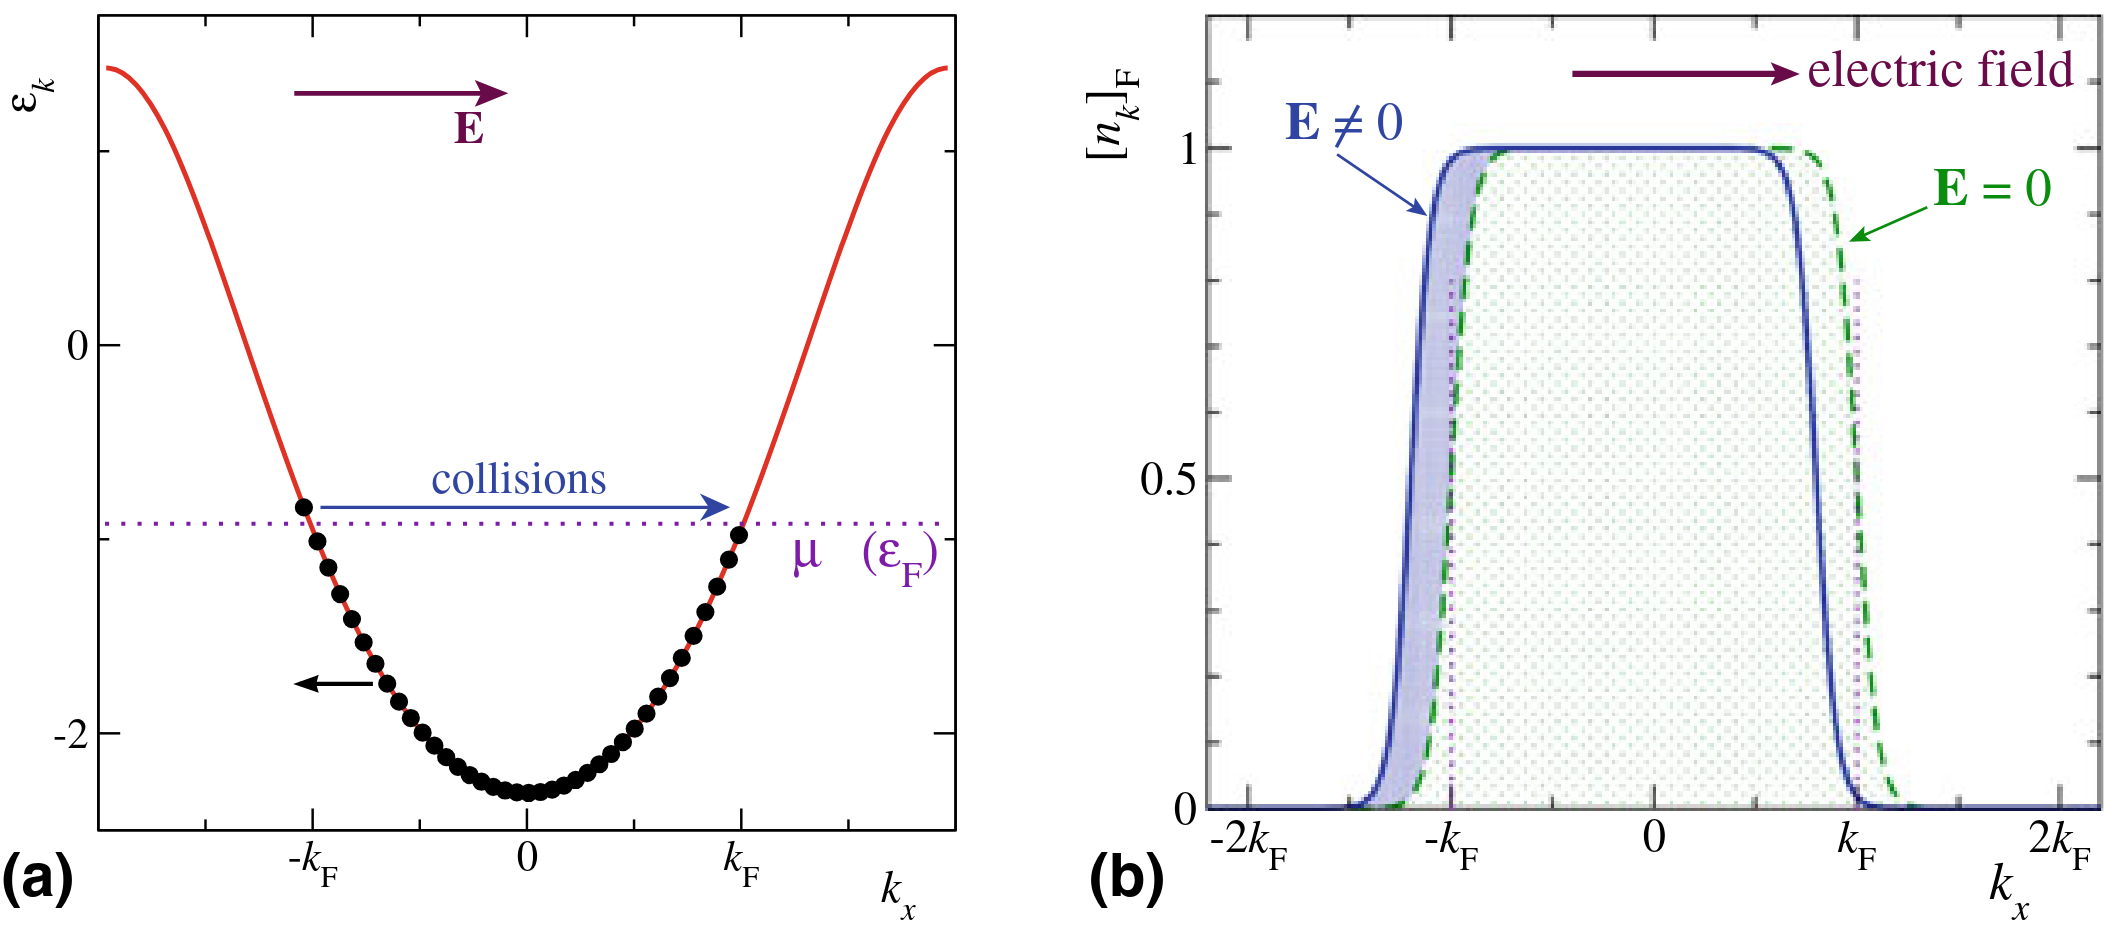
\includegraphics[width = 0.70 \textwidth]{therm-eq.png}
	\caption{Band occupation under the competing action oa a static electric field and collition with crystal defects and phonons.}
	\label{therm-eq}
\end{figure}
\begin{figure}
	\centering
	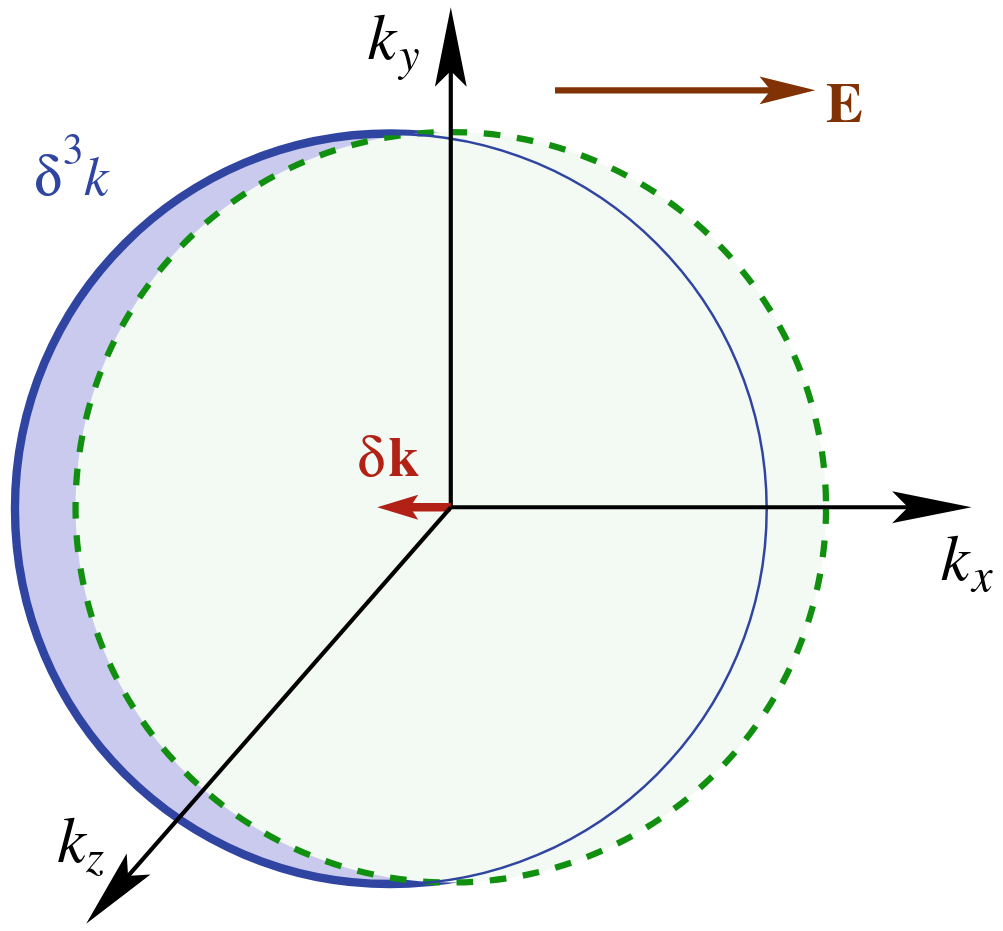
\includegraphics[width = 0.30 \textwidth]{fermi-sphere.png}
	\caption{Shift of the Fermi surface induced by a static electric field.}
	\label{f-sph}
\end{figure}

\subsubsection{Semiconduttori}

Negli isolanti, a differenza dei metalli, la densità dei portatori di carica (e dunque la conduttività elettrica) è proporzionale alla temperatura: oltre una certa temperatura, però, il moto dei portatori viene fortemente perturbato dall'agitazione termica, dunque $ \sigma $ torna a diminuire con l'aumentare di $ T $. Gli isolanti che a temperatura ambiente presentano una piccola conducibilità elettrica a temperatura ambiente (invece di $ \sigma = 0 $) vengono chiamati \textit{semiconduttori}: questi sono tipicamente cristalli in cui la gap tra la banda di valenza e quella di conduzione è larga $ \sim 1\ev $ a temperatura ambiente (es.: $ \ch{Si} $, $ \ch{Ge} $, etc.). \\
I semiconduttori presentano delle strutture cristalline diverse tra loro e, in virtù di queste differenze chimico-strutturali, le energy bands elettroniche di semiconduttori diversi presentano differenze qualitative e quantitative. In particolare, detti $ E_c $ il minimo della banda di conduzione ed $ E_v $ il massimo della banda di valenza, la gap $ \Delta = E_c - E_v $ può essere diretta, se $ E_c $ ed $ E_v $ sono nello stesso punto $ \ve{k} $, o indiretta, se si trovano in punti differenti. Dato che i fotoni, essendo massless, trasportano un momento piccolo, le transizioni ottiche coinvolgono sempre gap dirette: le transizioni indirette sono invece mediate da fononi, i quali però determinano interazioni al second'ordine poco probabili. I materiali a \textit{gap diretta} sono quelli in cui la gap più piccola è quella diretta, mentre i materiali a \textit{gap indiretta} hanno come gap minima quella indiretta: un esempio di quest'ultimi è il silicio, che ha una gap diretta $ \sim 3\ev $ ed una indiretta $ \sim 1\ev $.

\paragraph{Semiconduttori intrinseci}

\begin{figure}
	\centering
	\includegraphics[width = 0.50 \textwidth]{band-dens.png}
	\caption{Sketch of the density of electronic states in a crystal.}
	\label{band-dens}
\end{figure}

Nei semiconduttori intrinseci, ovvero cristalli perfetti (a meno di impurità entropiche), la conducibillità elettrica è determinata dall'eccitazione termica di una parte di elettroni dalla banda di valenza a quella di conduzione. La densità numerica media di elettroni attivi è quindi:
\begin{equation*}
	\frac{[n_c]}{V} = \frac{1}{V} \int_{E_c}^\infty \dd E\, g(E) [n_E]_\text{F} = \frac{1}{V} \int_{E_c}^\infty \dd E \frac{g(E)}{e^{\beta (E - \mu)} + 1}
\end{equation*}
Uno sketch della densità di stati $ g(E) $ è riportato in Fig. \ref{band-dens}. Inoltre, si può approssimare il potenziale chimico nei pressi del punto medio della gap tra banda di valenza e banda di conduzione: essendo $ \Delta \gg k_\text{B} T $ (si noti che $ 1\ev $ corrisponde a circa $ 12'000 \,\text{K} $), allora $ E_c - \mu \approx \frac{\Delta}{2} \gg k_\text{B} T $. Si può dunque approssimare:
\begin{equation*}
	[n_E]_\text{F} = \frac{1}{e^{\beta (E - \mu)} + 1} \simeq e^{- \beta (E - \mu)} = e^{- \beta (E_c - \mu)} e^{- \beta (E - E_c)}
\end{equation*}
Il prefattore è piccolo ed indipendente dall'energia, dunque è uguale per tutti gli elettroni nella banda: la distribuzione elettronica si riduce quindi ad una distribuzione di Boltzmann (limite a bassa densità, in quanto il gas elettronico è estremamente rarefatto in questo contesto). Espandendo attorno al minimo della banda di conduzione, inoltre, si trova:
\begin{equation*}
	E = E_c + \frac{1}{2} \sum_{\alpha,\beta = 1}^3 \frac{\pa^2 E_{c,\ve{k}}}{\pa k_\alpha \pa k_\beta}\bigg\vert_{\ve{k}_\text{min}} (\ve{k} - \ve{k}_\text{min})_\alpha (\ve{k} - \ve{k}_\text{min})_\beta + \dots \,= E_c + \frac{\hbar^2}{2m_\text{eff}} \abs{\ve{k} - \ve{k}_\text{min}}^2 + \dots
\end{equation*}
L'energia d'eccitazione $ \Delta E = E - E_c $ ha quindi la forma dell'energia cinetica di una particella libera di massa $ m_\text{eff} $ (massa effettiva valutata in $ \ve{k}_\text{min} $) e numero d'onda calcolato rispetto a $ \ve{k}_\text{min} $. Di conseguenza, la densità degli stati di conduzione (a meno dello spin) è data dall'Eq. \ref{eq:en-deg}:
\begin{equation*}
	g_\text{tr}(E) = \frac{V m_\text{eff}^{3/2}}{\sqrt{2} \pi^2 \hbar^3} \sqrt{E - E_c}
\end{equation*}
Si può così esplicitare la densità numerica degli elettroni attivi:
\begin{equation*}
	\begin{split}
		\frac{[n_c]}{V}
		& = \frac{1}{V} \int_{E_c}^\infty \dd E \frac{g(E)}{e^{\beta (E - \mu) + 1}} \simeq \frac{e^{-\beta (E_c - \mu)}}{V} \int_{E_c}^\infty \dd E\, g_s g_\text{tr}(E) e^{-\beta (E - E_c)} \\
		& = e^{\beta (E_c - \mu)} \frac{\sqrt{2} m_\text{eff}^{3/2}}{\pi^2 \hbar^3} \int_0^\infty \dd E\, \sqrt{E} e^{-\beta E} = e^{\beta (E_c - \mu)} \frac{\sqrt{2} m_\text{eff}^{3/2}}{\pi^2 \hbar^3} \frac{\sqrt{\pi}}{2 \beta^{3/2}} = e^{\beta (E_c - \mu)} \left[ \frac{m_\text{eff} k_\text{B} T}{\sqrt[3]{2} \pi \hbar^2} \right]^{3/2}
	\end{split}
\end{equation*}
Per il silicio a $ T = 300 \,\text{K} $ si trova una densità numerica di elettroni attivi $ \sim 10^{15} \,\text{m}^{-3} $, 14 ordini di grandezza più piccola della tipica densità per i metalli. Si noti, però, che questa densità dipende esponenzialmente da $ T^{-1} $, ed infatti già a $ T = 600\,\text{K} $ si ha densità $ \sim 10^{29} \,\text{m}^{-3} $: a temperatura ambiente, i semiconduttori hanno resistività di vari ordini di grandezza maggiori rispetto ai metalli, ma la forte sensibilità dalla temperatura li rende ottimi sensori termici.

\paragraph{Semiconduttori estrinseci}

Dato che a temperatura ambiente la resistività dei semiconduttori intrinseci è talmente alta che si comportano da isolanti, per aumentarne la conduttività si aggiungono elementi di altro tipo in un processo detto \textit{drogaggio} (inserzione di impurità nel cristallo).












\end{document}
